\documentclass{wissdoc}

%% --------------------
%% |     Packages     |
%% --------------------

\usepackage[utf8]{inputenc}

% Weitere packages: (Dokumentation dazu durch "latex <package>.dtx")

%\usepackage{bibgerm}
%\usepackage[backend=biber]{biblatex} 
\usepackage{csquotes} 
\usepackage{tabularx}
\usepackage{booktabs}
\usepackage{multirow}
%\usepackage{tocbibind}
\usepackage{siunitx}
\usepackage{xcolor}
\usepackage{textcomp}
\usepackage{listings}
\usepackage{newfloat,caption}
\usepackage{subcaption}
\usepackage{footnote}
\usepackage{rotating}
\usepackage{pgfplots}
\usepackage{pgfplotstable}
\usepackage{url}
\usepackage{boxhandler}
\usepackage{tabu}
\usepackage{amssymb}
%\usepackage{subfig}
%\usepackage{subcaption}
\usepackage{caption}
\usepackage{subcaption}
%\usepackage[plainpages=true]{hyperref}
\usepackage[space]{grffile}
\usepackage{pdfpages}
%\usepackage[numbers,sort&compress]{natbib}
\usepackage[backend=bibtex,natbib=true,hyperref=true,doi=false,url=false]{biblatex}
% \usepackage{varioref}
% \usepackage{verbatim}
\usepackage{float}    %z.B. \floatstyle{ruled}\restylefloat{figure}
%\usepackage[hidelinks]{hyperref}
% \usepackage{subfigure}
% \usepackage{fancybox} % für schattierte,ovale Boxen etc.
% \usepackage{tabularx} % automatische Spaltenbreite
% \usepackage{supertab} % mehrseitige Tabellen
% \usepackage[svnon,svnfoot]{svnver} % SVN Versionsinformation 

% My packages
\usepackage{graphicx}

%% --------------------
%% |     Settings     |
%% --------------------

% Settings: Titlepage, Comments, etc.
\pgfplotsset{compat=newest}

% Settings for Titlepage
\hypersetup{
	colorlinks,
  citecolor=black,
  filecolor=black,
  linkcolor=black,
  urlcolor=black,
 pdfauthor={Tobias Kaessmann},
 pdftitle={Investigation of touch for
passive haptic Braille learning}
 pdfsubject={Not set},
 pdfkeywords={Not set}
}
\DeclareFloatingEnvironment[fileext=frm,placement={!ht},name=Listing,within=section]{listing}

% Print URLs not in Typewriter Font
\def\UrlFont{\rm}

% \newcommand{\specialcell}[2][c]{%
%   \begin{tabular}[#1]{@{}c@{}}#2\end{tabular}}
\newcommand{\specialcell}[2][c]{%
  \begin{tabular}[#1]{@{}l@{}}#2\end{tabular}}

\newcommand\todo[1]{\textcolor{red}{TODO: #1}}

\newcommand\hlcode[1]{\textcolor{red}{#1}}

\newcommand\citeable[1]{\textcolor{green}{\hl{citeable: #1}}}

\newcolumntype{\$}{>{\global\let\currentrowstyle\relax}}
\newcolumntype{^}{>{\currentrowstyle}}
\newcommand{\rowstyle}[1]{\gdef\currentrowstyle{#1}%
  #1\ignorespaces
}

% Comments
\newif\ifcomment
%\commenttrue

% Leerseite ohne Seitennummer, nächste Seite rechts
\newcommand{\blankpage}{
 \clearpage{\pagestyle{empty}\cleardoublepage}
}

% Bibliography
\addbibresource{bib/references.bib}

%% --------------------------------------------------------------------------------
%% |                           BEGINNING OF DOCUMENT                              |
%% --------------------------------------------------------------------------------
\usepackage[acronym]{glossaries}


\newacronym{phl}{PHL}{Passive Haptic Learning}
\newacronym{bct}{BCT}{Bone conducting transducer}
\newacronym{mmt}{MMT}{Mobile Music Touch}
\newacronym{vsr}{VSR}{Vibrotactile Skin Reading}
\newacronym{ost}{OST}{Prioritized Overlapping Spatiotemporal Sequence}
\newacronym{tvi}{TVI}{Teacher of Students with Visual Impairments}
\newacronym{sci}{SCI}{spinal cord injury}
\newacronym{pdm}{PDM}{Pulse Duration Modulation}
\newacronym{mvp}{MVP}{Minimal Viable Prototype}
\newacronym{seq}{SEQ}{Sequential encoding}

\newacronym{csgf}{Chi-Square GF}{Chi-Square Goodness-of-Fit Test}
\newacronym{emgf}{Exact MGF}{Exact Multinomial Goodness-of-Fit Test}
\newacronym{mwu}{MW U test}{Mann-Whitney U Test}

\newacronym{pca}{PCA}{Principal component analysis}

\usepackage{braille}
 \usepackage[utf8]{inputenc}
\usepackage[T1]{fontenc}

\makeglossaries

\begin{document}

%% ----------------------
%% |     Title Page     |
%% ----------------------
\frontmatter
\pagenumbering{roman}
\ifnotdraft{
 
\includepdf[pages=-]{titelseiten.pdf}
}

%% ----------------------------
%% |     Table of Content     |
%% ----------------------------

\ifnotdraft{
\pagenumbering{roman}
{\parskip 0pt\tableofcontents} % toc bitte einzeilig
\listoffigures
\listoftables
}
\cleardoublepage
{\pagestyle{empty}
~
\cleardoublepage}
%\thispagestyle{empty}

%% ------------------
%% |     Content    |
%% ------------------

\graphicspath{{src/}}

\mainmatter
\pagenumbering{arabic}
\printglossaries{}
% \chapter{Introduction}
\label{ch:Introduction}

Learning Braille remains a significant challenge for blind people or visually impaired individuals, especially those who lose vision later in life \cite{Seim2014a}. Braille is more than just a reading system; it is a critical literacy medium that is directly correlated with better educational outcomes and employment opportunities \cite{Seim2014a, Ryles1996}. Ryles et al. note that Braille is the primary language of literacy for blind individuals and is associated with stronger reading habits and greater likelihood of pursuing post-secondary education \cite{Ryles1996}. In addition, daily use of Braille has been shown to positively impact employment, salary, and self-esteem \cite{Bell2013}. Despite these clear benefits, only 10 percent of blind individuals learn Braille due to the lack of certified instructors and resources. And 74\% of blind individuals are unemployed \cite{Seim2014a}.

The challenges of Braille literacy are further compounded by the wide variability of teaching approaches, each requiring learners to have ample opportunities to use and develop their understanding of Braille contractions \cite{Swenson1999}. Modern technologies such as text-to-speech are able to help visually impaired people participate in active life, but also cause neglect in Braille instruction \cite{Seim2014a}. However, excessive reliance on audio learning can negatively affect essential literacy skills such as spelling and composition \cite{Foulke1979}, as full reliance on audio technology is inconsistent with the broader definition of literacy, which also includes writing \cite{tuttle1996point}.

In light of these barriers to traditional Braille instruction, several Braille learning devices such as gloves have been invented like the devices by Zaman et al. \cite{Zaman2019}, Ozioko et al. \cite{Ozioko2017}, An \cite{An2004} Cho et al. \cite{Cho2002} and other such as Seim et al. \cite{Seim2014a, Seim2014, Seim2015}, Yang et al. \cite{Yang2017} or Forsyth et al.\cite{Learning2024}.
And also different teaching / aquiring methods such as active and passive learning. In our opinion, \gls{phl} offers a promising solution due to the lack of active attention needed. \Gls{phl} enables individuals to learn motor tasks, such as Braille typing, through tactile stimulation without requiring active attention. Research teams have leveraged this concept to design assistive gloves that teach Braille through muscle memory, a form of procedural memory that allows individuals to unconsciously retain skills over time \cite{Yang2017,Seim2015}. By using \gls{phl}, individuals can passively learn Braille while performing everyday activities, such as walking or commuting, reducing the time and effort required for instruction \cite{Yang2017}.

The potential of \gls{phl} to accelerate Braille learning is further supported by research into the neuroplastic changes that occur during the process. Blind individuals who learn Braille experience cortical changes, including enlargement of the sensorimotor area associated with the reading finger and the recruitment of the occipital cortex, which formerly processed visual information, for tactile tasks \cite{Hamilton1998a}. By providing continuous, passive tactile stimulation, \gls{phl} systems may enhance these neuroplastic processes, making Braille learning more efficient. In doing so, \gls{phl} offers a viable solution to address the "crisis" in Braille literacy \cite{Seim2014a}, providing an innovative method for improving literacy and independence for those who are blind or visually impaired.
However, many open questions remain in this domain, such as: \textit{\textbf{R1:} Is there a difference between using affective touch and discriminative touch for learning Braille?} and \textit{\textbf{R2:} How should information be encoded in the glove to be conveyed efficiently to the learner?} These are the questions this thesis aims to address, with the goal of easing the burden of learning Braille and enabling more individuals to embrace a life of literacy."
  
% %Let's cite \cite{battlenet}. 

% \section{Dummy Table}
% \label{sec:dummy_table}

% \begin{table}[h!]
% \centering
% \begin{tabular}{c c c} 
%  cell1 & cell2 & cell3 \\ 
%  cell4 & cell5 & cell6 \\  
%  cell7 & cell8 & cell9    
% \end{tabular}
% \caption{Dummy Table}
% \label{table:dummy_table}
% \end{table}


% \section{Dummy Image}
% \label{sec:dummy_img}

% \begin{figure}[h]
% \centering
% 
\includegraphics[width=0.5\textwidth]{src/logos/TECO_KIT.pdf}
% \caption{Dummy Image}
% \label{table:dummy_img}
% \end{figure} %2
% \chapter{Background \& Related Work}
\label{ch:Background}

\newcommand{\ea}[2]{#1 \text{et al.} #2}


%50-100 pages
%Introduction
%Hardware and such narrow down target users - potential users
%Adults make not sense using touching learning ()
%Adult vs child group comparison - maybe change some papers

%Not always refers to articles, but also to commercial products
%Create own citation based on minimum inforamation
%Summarise applications which are out there

%Is there a gold standard for braille learning for sighted people

%Haptic braille learning paper

%Special experts could use the application
%Let expert try out final report
%Let try out potential users (specify the potential users) —> sight adults \ exclude non adult literature also in design 
%Backward chain of papers - commonly used method.

%Intro, discussion 10
%30 methods
%30 related work

\section{Passive learning}
Learning is often perceived as an active and purposive process; however, this is not always the case. In addition to active learning, there exists a form of passive learning, which stands in contrast to the active approach. Passive learning is often described as being \enquote{caught rather than taught} \cite{krugman1970passive}, emphasizing its effortless nature. This lack of effort is attributed to the absence of resistance, meaning that neither motivation nor interest is necessary for the acquisition of this type of knowledge \cite{Zukin1984}.
Furthermore, passive learning has been characterized as “typically effortless, responsive to animated stimuli, amenable to artificial aids to relaxation, and marked by an absence of resistance to what is learned” \cite{Huang2008,krugman1970passive}. This suggests that passive learning can occur in environments where learners are exposed to stimuli without actively engaging in the learning process.
Zukin et al. \cite{Zukin1984} demonstrated that exposure to media-rich environments can lead to information being acquired passively. In their study, they examined two groups of subjects who were not initially interested in political information. They found that subjects who were exposed to political content through a media-rich environment were 40\% more likely to acquire the information compared to those living in media-poor environments \cite{zukin1984passive, Huang2008}.
Later research by Huang et al. \cite{Huang2008} extended the concept of passive learning to the acquisition of physical skills. The success of this study contributed to the introduction of the term \gls{phl} \cite{Pescara2019}, which further encapsulates the potential for learning in contexts where active engagement is minimal or absent.
Over the years a significant body of research has been dedicated to the exploration of \gls{phl}. It spanned a wide range of applications, including piano learning \cite{Huang2008, Kohlsdorf2010, Seim2015b, Donchev2021, Fang2023a, Fang2023}, the acquisition of typing skills \cite{Seim2014, Seim2017, Seim2014a, Learning2024}, the learning of Braille \cite{Seim2014a, Learning2024}, Morse code \cite{Seim2016a, Seim2018, Pescara2019}, multi-limb rhythm coordination \cite{Bouwer2011, Holland2010}, skin reading \cite{Luzhnica2016, Luzhnica2018}, and even the effects of \gls{phl} on spinal cord injury (SCI) rehabilitation \cite{Markow2010}.


%-----
\subsection*{Distraction Task}
\begin{table}[!ht]
\centering
\resizebox{\columnwidth}{!}{
\begin{tabular}{|l|l|l|l|l|l|}
    \hline
        \textbf{Paper name} & \textbf{Game} & \textbf{Learning Time} \\ \hline
        \ea{Aveni}{\cite{Aveni2019}}& & & & SpikeDislike2&4 * 10 min\\ \hline
        \ea{Caulfield}{\cite{Learning2024}} &  Not mentioned & 10 min \\ \hline
        \ea{Fang}{\cite{Fang2023}} &  Gweled  & 30 min \\ \hline
        \ea{Fang}{\cite{Fang2023a}} &  Tetris & 15 min \\ \hline
        \ea{Donchev}{\cite{Donchev2021}} &  Gweled & 20 min \\ \hline
        \ea{Hsu}{\cite{Hsu2021}} & Not mentioned & 30 min \\ \hline
        \ea{Pescara}{\cite{Pescara2019}} & \specialcell{Gweled\\ Open Hexagon} & \specialcell{20 min \\(5 min training/character)} \\ \hline
        \ea{Luzhnica}{\cite{Luzhnica2018}} &  Snake Game & 32 min \\ \hline
        \ea{Seim}{\cite{Seim2018}} &  Fritz & 8 or 16 min \\ \hline
        \ea{Seim}{\cite{Seim2017}} &  Fritz & 15 min \\ \hline
        \ea{Seim}{\cite{Seim2016a}} &  Fritz & 20 min \\ \hline
        \ea{Seim}{\cite{Seim2015b}} &  Fritz & 20 min \\ \hline
        \ea{Seim}{\cite{Seim2014}} & Memory Card Game & 30 min \\ \hline
        \ea{Seim}{\cite{Seim2014a}} & Fritz &  30 min \\ \hline
        \ea{Bouwer}{\cite{Bouwer2011}} &  Reading Comprehension &  30 min \\ \hline
        \ea{Kohlsdorf}{\cite{Kohlsdorf2010}} &  \specialcell{Watching a film\\Playing memory\\Walking a path} & 5 min \\ \hline
        \ea{Huang}{\cite{Huang2010}} & \specialcell{Daily task (pilot study)\\ PSAT/SAT (main study)} & 30 min \\ \hline
        \ea{Pala}{\cite{Vaio6810}} &  Not mentioned & 15-60 min \\ \hline
        \ea{Huang}{\cite{Huang2008}} & \specialcell{Daily task\\ (Reading book/paper, typing at desk)} & 30 min \\ \hline
    \end{tabular}
    
}
\caption{Distraction tasks leveraged in previous literature.}
\label{tab:distraction_tasks}
\end{table}

Apart from the primary challenges of learning new skills or rehabilitation, much of the focus in \gls{phl} research has been on distraction tasks, which are crucial to its main selling point. Distraction tasks are those that can be performed concurrently while the primary learning process takes place, allowing the acquisition of information to occur passively. We compared the distraction tasks used in previous literature, along with the time participants spent learning, and summarized them in \autoref{tab:distraction_tasks}.

In earlier \gls{phl} research, reading comprehension tests \cite{Huang2008, Huang2010, Kohlsdorf2010} were commonly employed as the distraction task. However, this method has largely fallen out of favour. During the development of the \gls{mmt} framework, Kohlsdorf et al. \cite{Kohlsdorf2010} tested three different tasks: watching a film (audio-visual stimulation), playing a memory game (active memory engagement), and walking a designated path (body motion). These tasks were chosen to represent common everyday activities such as relaxing, thinking, and walking.

The results showed no statistically significant difference in the number of \gls{phl} sessions required across the different tasks. However, individual differences emerged, with some participants finding certain tasks more challenging than others. Rhythm retention was slightly better after the memory game condition compared to the film condition, though no condition was significantly better or worse overall. Participants reported similar subjective workloads across all conditions, suggesting that the type of primary task does not significantly impact the effectiveness of \gls{phl} in learning piano sequences. The study concluded that while the type of primary task may influence individual performance, there is no clear evidence that one task is superior to others in enhancing \gls{phl} effectiveness. This suggests that \gls{phl} can be integrated into various everyday activities without being significantly hindered by the nature of the concurrent task.

This was also investigated by \citet{Pescara2019}, who found that the difficulty level of distraction tasks, such as the games Gweled (easy) and Open Hexagon\footnote{Open Hexagon: \url{https://vittorioromeo.info/Downloads/}} (hard), did not significantly influence learning outcomes \cite{Pescara2019}. However, Pescara et al. also noted that participants reported increased fatigue over the course of the study due to the prolonged focus required by these games. This finding suggests that future research should explore alternative distraction tasks that are engaging enough to divert attention from \gls{phl}, yet unlikely to induce fatigue during extended periods—a challenge that remains difficult to address.

More recent studies have shifted their focus to other tasks, such as playing the game 'Fritz'\footnote{Fritz!: \url{www.gamesgames.com/game/fitz.}}, which has become the most frequently used alternative, appearing in five studies, followed by the game 'Gweled,'\footnote{Gweled: \url{https://gweled.org}} which has been utilized in three studies. \autoref{tab:distraction_tasks} provides an overview of the games used as distraction tasks in previous literature.


\subsection*{PHL Duration}
Another crucial factor is the duration of the distraction task and the period during which passive learning occurs, as this may directly influence the effectiveness of the \gls{phl} process. As shown in \autoref{tab:distraction_tasks}, most studies employ a standard learning period of 30 minutes before subjects undergo further testing or evaluation. Close behind, several studies opt for a slightly shorter 20-minute learning period. However, there is significant variability in session lengths, ranging from as brief as 5 minutes to as long as 60 minutes, indicating no clear consensus on the optimal duration. To explore this further, Seim's study \cite{Seim2018} highlighted the benefits of extended learning time. The study demonstrated a notable improvement in learning Morse code between 8-minute and 16-minute exposure conditions, suggesting that longer exposure periods may be more advantageous.

\subsection*{Overlearning}
Another aspect closely tied to learning duration is the concept of overlearning. Overlearning refers to the deliberate overtraining of an already learned task, aiming to achieve error-free performance \cite{Krueger1929}. Numerous psychological studies have examined its effects, particularly on retention \cite{Krueger1929, Driskell1992}. While overlearning can enhance retention, it may also have adverse effects, such as degrading performance, as demonstrated by Langer et al. \cite{Langer1979}.

In the context of \gls{phl}, Donchev et al. \cite{Donchev2021} deliberately avoided overlearning, citing its unpredictable effects on long-term retention and the potential for distorted results. To mitigate this, they halted the learning session once participants achieved an accuracy of 90% or higher.

However, not all studies have avoided overlearning. For example, Seim et al. \cite{Seim2016, Seim2014a} included overlearning in their experimental design. In their full alphabet study \cite{Seim2014a}, they specifically investigated its effects. Conversely, in another study \cite{Seim2015}, they avoided overlearning to prevent ceiling effects on shorter phrases. This suggests that the decision to include overlearning in some studies was likely a deliberate choice tailored to the research objectives.

\subsection*{Chunking}
When learning information, it is often presented piece by piece. This is called \enquote{chunking} and it is a critical concept in cognitive science, especially in memory and learning processes. It involves breaking large pieces of information into smaller, more manageable units to enhance retention. \ea{Miller}{\cite{miller1956}} first observed that the average person can hold about seven items in working memory, and that chunking helps organize information into meaningful patterns. \ea{Laird}{\cite{Laird1984}} emphasized that chunks are the basic units of human memory, allowing the brain to retrieve information from long-term memory more efficiently. \ea{Thalmann}{\cite{Thalmann2019}} demonstrated that chunking reduces working memory load, benefiting recall as long as the chunks consist of unique elements.

In passive learning, chunking is widely used to improve learning and retaining efficiency. \ea{Markov}{\cite{Markow2010}} divided note sequences into four passages of 10-15 notes each. \ea{Seim}{\cite{Seim2014}} found that random presentation of letters and words did not aid learning, highlighting that chunk size and learning time are crucial factors in passive learning. They taught phrases one at a time. Similarly, Seim et al. \cite{Seim2014a} applied chunking in language learning with phrases like "add a bag" (AAB) and "hike fee" (HF), which involved 15-18 vibrations and 3-4 characters. These phrases were comparable in length to previous work on \gls{phl} for piano \cite{Kohlsdorf2010} and typing \cite{Seim2014}.
Seim et al. continued to use chunking in \cite{Seim2015} to teach 4-8 note sequences with chords, finding that optimal learning occurred in sets of 10-17 stimuli. They also used chunking to teach Morse code via a \gls{bct} introducing one word at a time from the sentence "the quick brown fox jumps over the lazy dog" \cite{Seim2016}.
In their keyboard learning research, Seim et al. \cite{Seim2017} employed row-wise in contrast to the widely used word-wise chunking. Additionally, in their smartwatch-based Morse code study, Seim et al. presented phrases in manageable chunks for improved retention \cite{Seim2018}.

\ea{Luzhnica}{\cite{Luzhnica2018}} applied chunking to teach 10 letters, repeating each letter four times in multiple rounds, while \ea{Prescara}{\cite{Pescara2019}} used chunking to reduce Morse code training time by dividing the 26 patterns into three sets.

Moreover, studies such as the study of \ea{Sargent}{\cite{sargent2010chunking}} further support chunking’s role in memory, showing that participants recalled spatial information more accurately when it was grouped into smaller chunks.

However not every related work used chunking as a means of transmitting information to the participants. \ea{Kohlsdorf}{\cite{Kohlsdorf2010}}, \ea{Donchev}{\cite{Donchev2021}}, Fang et al. \cite{Fang2023a, Fang2023}, and Huang et al. \cite{Huang2008} did not use chunking for note sequences of 6-10 notes, as it was likely unnecessary due to the short sequence length.

\subsection*{Timing}
Another important consideration is the timing of audio and sensory input—primarily in the form of vibrations—used in previous studies. Cognitive processing can be hindered when individuals are required to perform two perceptual tasks simultaneously, as shown by Gescheider et al. \cite{Gescheider1975}. To mitigate this issue, most \gls{phl} research incorporates a delay or offset between audio and sensory inputs, although the specific timings vary across studies \cite{Seim2014, Seim2017, Luzhnica2018, Fang2023a}.

For instance, Seim et al. \cite{Seim2014} introduced a 100ms offset, where the audio was followed shortly by the vibration sequence corresponding to the word being learned. In a later study \cite{Seim2016}, they extended this offset to 1 second, before eventually eliminating it altogether in \cite{Seim2017}, where stimuli were presented immediately after the text was spoken. Similarly, Luzhnica et al. \cite{Luzhnica2018} implemented a brief 50ms delay between auditory and vibrotactile cues.

By contrast, Pescara et al. \cite{Pescara2019} adopted a simultaneous approach, delivering both sensory input and audio at the same time. Fang et al. \cite{Fang2023a} opted for a short offset of a few seconds, ensuring that auditory signals were delivered during pauses of the tactile signals, and vice versa.





\subsection*{Glove Design}
\begin{table}[!ht]
\centering
\resizebox{\columnwidth}{!}{
    \begin{tabular}{|l|l|l|l|l|}
    \hline
        \textbf{Paper name} & \textbf{Location} & \textbf{Device} & \textbf{Actuator} & \textbf{Chorded input} \\ \hline
        \ea{Aveni}{\cite{Aveni2019}}& Proximal phalanx (dorsal side)& Fingerless Glove & Vibration &\specialcell{Yes (Staggered)} \\ \hline
        \ea{Caulfield}{\cite{Learning2024}} & Center proximal phalanges & Fingerless Glove & Vibration & Yes (didn't work) \\ \hline
        \ea{Fang}{\cite{Fang2023}} & Proximal phalanges close to joint & Velcro bands & \specialcell{Dragging\\ Tapping\\ Vibration} & No \\ \hline
        \ea{Fang}{\cite{Fang2023a}} & \specialcell{Intermediate phalanges\\ Bottom of distal phalanx (thumb)} & Cotton glove & Vibration & No \\ \hline
        \ea{Fang}{\cite{Fang2022}} & Below proximal interphalangeal & Plastic glove & Vibration & No \\ \hline
        \ea{Fang}{\cite{Fang2022a}} & \specialcell{Index Finger Proximal Phalanges\\ Index Finger Intermediate Phalanges\\ Outer Wrist and Inner Wrist} & \specialcell{Self-adhesive tape\\ Elastic strap} & \specialcell{Dragging\\ Tapping\\ Vibration} & No \\ \hline
        \ea{Fang}{\cite{Fang2022b}} & 3 Arm positions & Elastic band & \specialcell{Dragging\\ Tapping\\ Vibration} & No \\ \hline
        \ea{Donchev}{\cite{Donchev2021}} & \specialcell{Above proximal phalanges\\ Near interphalangeal joint} & Glove (Soft, Stretchy) & Vibration & No \\ \hline
        \ea{Hsu}{\cite{Hsu2021}} & Fingertips & Velcro-fastening straps & Vibration & No \\ \hline
        \ea{Pescara}{\cite{Pescara2019}} & Wrist & Velcro tape fastening & Vibration & No \\ \hline
        \ea{Luzhnica}{\cite{Luzhnica2018}} & Hand (back) & Glove & Vibration & \specialcell{Yes (partly)\\OST encoding} \\ \hline
        \ea{Seim}{\cite{Seim2018}} & Wrist & Smartwatch & Vibration & No \\ \hline
        \ea{Yang}{\cite{Yang2017}} & Fingertips & Glove & Vibration & Yes \\ \hline
        \ea{Seim}{\cite{Seim2017}} & Intermediate phalanges & Fingerless Glove & Vibration & No \\ \hline
        \ea{Seim}{\cite{Seim2016a}} & Head & Google Glass & \gls{bct} & No \\ \hline
        \ea{Seim}{\cite{Seim2015b}} & Proximal phalanges & Fingerless Glove & Vibration & \specialcell{Yes (Staggered)\\ like \ea{Seim}{\cite{Seim2014a}}} \\ \hline
        \ea{Seim}{\cite{Seim2014}} & Proximal phalanges & Fingerless Glove & Vibration & \specialcell{Yes (didn't work)\\ (Non-staggered)} \\ \hline
        \ea{Seim}{\cite{Seim2014a}} & Proximal phalanges & Fingerless Glove (stretchy) & Vibration & \specialcell{Yes (Staggered)} \\ \hline
        \ea{Bouwer}{\cite{Bouwer2011}} & Limbs & Velcro bands & Vibration & Yes \\ \hline
        \ea{Huang}{\cite{Huang2010}} & Proximal phalanges & Fingerless Glove (stiff) & Vibration & No \\ \hline
        \ea{Pala}{\cite{Vaio6810}} & \specialcell{Proximal phalanges (Version 1)\\ Intermediate phalanges (Version 2)} & \specialcell{Fingerless Glove (abandoned)\\ Patchwork Glove} & Vibration & No \\ \hline
        \ea{Kohlsdorf}{\cite{Kohlsdorf2010}} & Proximal phalanges & Fingerless Glove & Vibration & No \\ \hline
        \ea{Markow}{\cite{Markow2010}} & Proximal phalanges & \specialcell{Fingerless Glove (golf)\\Fingerless Open Flap Glove\\Velcro Finger Glove} & Vibration & No \\ \hline
        \ea{Huang}{\cite{Huang2008}} & Proximal phalanges & Fingerless Glove (golf) & Vibration & No \\ \hline
\end{tabular}
}
\caption{Overview of the devices in previous literature.}
\label{tab:devices}
\end{table}

As previous research shows, \gls{phl} is not only constrained to the hand, and there are several appliances, that facilitate the option of learning \gls{phl} such as smartwatches \cite{Seim2018}, wrist bands, google glasses \gls{bct} \cite{Seim2016a}, velcro bands at the limbs \cite{Bouwer2011} or even gloves as depicted in \autoref{tab:devices}.

Various haptic devices have been employed for \gls{phl}, including smartwatches \cite{Seim2018}, Google Glass \cite{Seim2016a}, and Velcro bands applied to the limbs \cite{Bouwer2011} (as can be seen in \autoref{tab:devices}). However, given that previous research has primarily focused on the hand, the glove has emerged as one of the most extensively studied devices for \gls{phl}, followed closely by vector bands, which are predominantly used on the fingers, some glove designs can be seen in \autoref{fig:glove_designs}. This trend may also be influenced by the significant number of studies centred on learning to play piano pieces.
Within this context, there are notable differences in the types of gloves used, such as fingerless gloves versus standard gloves, as seen in \autoref{fig:glove_designs}. A critical factor in selecting gloves for \gls{phl} is the placement of actuators. Fingerless gloves are often preferred due to their superior manual dexterity \cite{Huang2008}, allowing wearers to perform everyday tasks more easily (as demonstrated in the \gls{mmt} system \cite{Markow2010, Kohlsdorf2010, Huang2010}). Additionally, fingerless gloves are more adaptable to various hand sizes, ensuring that actuators can be precisely positioned \cite{Seim2014a, Seim2015b}.
Other important considerations for glove design include weight, breathability, flexibility, and coarseness, all of which contribute to the comfort of the device—an essential factor given the need for extended wear \cite{Markow2010, Kohlsdorf2010, Huang2010, Fang2023a}. These considerations might also explain the advantages of using velcro bands as an alternative to gloves.

Special gloves were also invented for braille learning such as the gloves by Yang et al. \cite{Yang2017} that use gloves with vibration at the fingertips for typing Taiwanese braille or \cite{Learning2024} Caulfield et al., which uses a haptic glove with vibration at the intermediate parallax for typing braille, or even Seim et al. \cite{Seim2014a} using a stiff glove \cite{Seim2014} as well as many more notable mentions such as the ones from Zaman et al. \cite{Zaman2019}, Ozioko et al. \cite{Ozioko2017}, An et al. \cite{An2004}, Cho et al. \cite{Cho2002}, however, they are not specialised for \gls{phl}, only for active learning.

\begin{figure}[!ht]
    \centering

    \includegraphics[width=\linewidth]{src/pictures/hand_haptics.drawio.png}
    \caption{Glove variants and designs used in previous works \cite{Donchev2021,Fang2023,Fang2023a,Huang2008,Huang2010,Learning2024,Luzhnica2016,Markow2010,Seim2014a,Seim2017,Seim2015b,Seim2014,Vaio6810}.}
    \label{fig:glove_designs}

\end{figure}



\subsection*{Actuator hand placement}
 \begin{figure}[!ht]
    \centering
    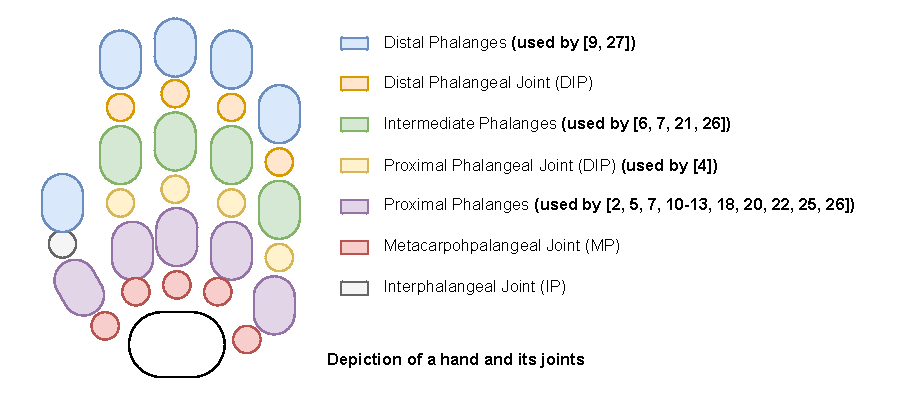
\includegraphics[width=\linewidth]{src/pictures/hand_Depiction.drawio.pdf}
    \caption{Actuator placement on the hand in previous works \cite{Learning2024,Fang2023,Fang2023a,Fang2022,Fang2022a,Donchev2021,Hsu2021,Yang2017,Seim2017,Seim2015b,Seim2014a,Seim2014, Huang2010, Vaio6810, Kohlsdorf2010, Markow2010, Huang2008}.}
    \label{fig:hand_depiction}
\end{figure}
The placement of actuators has undergone significant changes in recent research. While some studies have explored more unconventional approaches, such as the \gls{bct} used in Google Glass \cite{Seim2016a}, smartwatches \cite{Seim2018} worn on the wrist, or Velcro bands applied to the limbs for rhythm learning \cite{Bouwer2011, Holland2010}, the majority of research has focused on the skin of the hand (and occasionally the arm) as a successful site for input.
In particular, the placement of actuators on the fingers has shown that targeting the proximal phalanges is advantageous \cite{Fang2022a}, but research also explored other areas, such as the fingertips \cite{Yang2017} or even the wrist or back of the hand. \autoref{fig:hand_depiction} shows the different hand placements and their corresponding papers.
Research from Fang suggested, that the response time at the finger is shorter than for the wrist for the stimuli (vibration, taping and stroking) and the perception accuracy at the finger is significantly more accurate than at the wrist, moreover, their experimental results indicated, that the Finger Phalanx achieves higher accuracy than the Outer Wrist \cite{Fang2022a}.

\subsection{Human skin and the influences of stimulus}
\begin{figure}
    \centering
    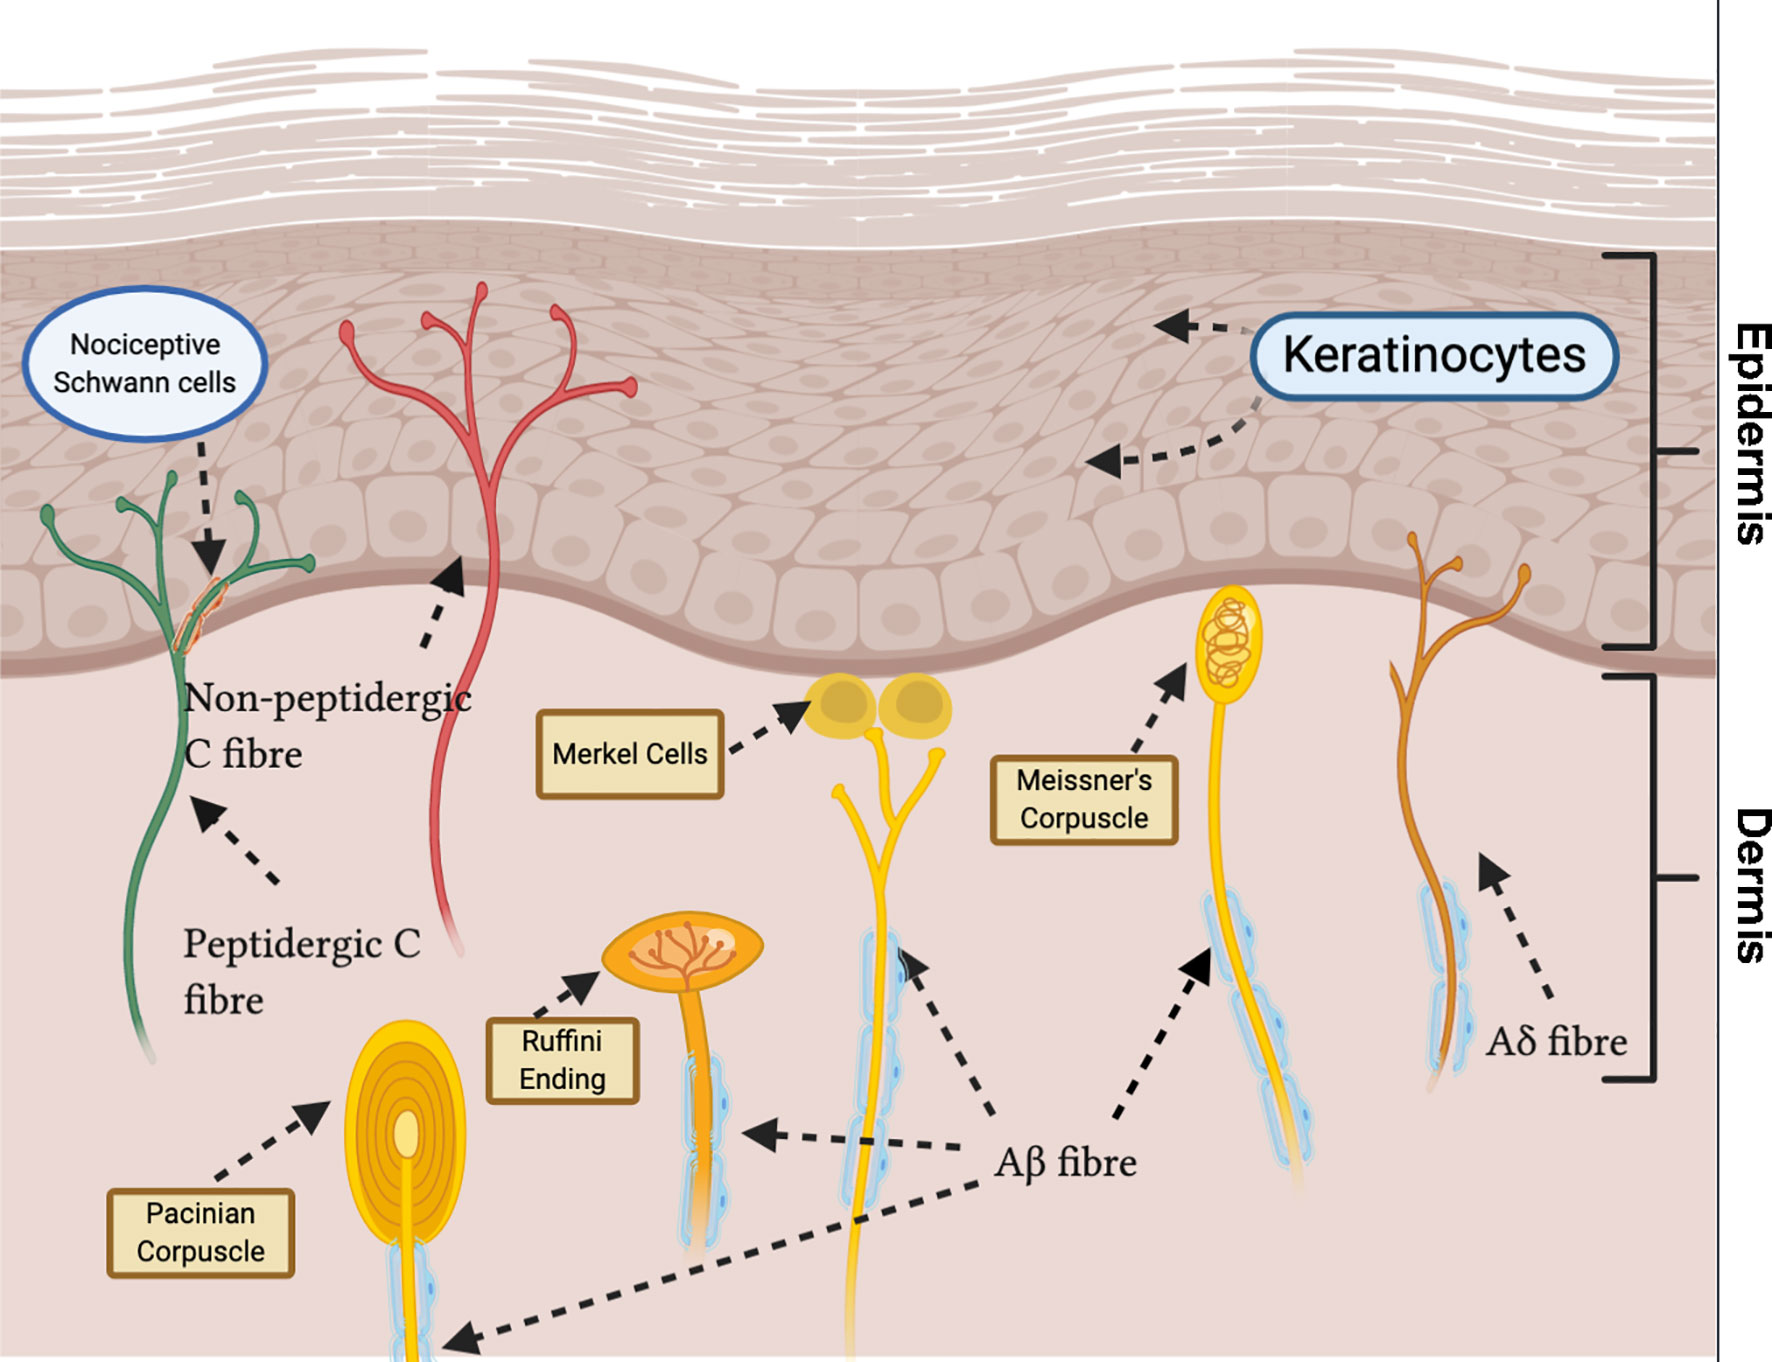
\includegraphics[width=0.7\linewidth]{src//pictures/skin.jpg}
    \caption{Depiction of the human skin \cite{lowy2021cutaneous}.}
    \label{fig:skin_image}
\end{figure}

The human skin, the largest and most visible organ of the body, serves as a versatile interface for perceiving a wide range of sensations. Beyond its protective functions, the skin provides sensory input from the environment and acts as a medium for communication and feedback. It is capable of detecting mechanical, thermal, chemical, and electrical stimuli, which generate sensations such as pressure, vibration, temperature, and pain. This diversity makes touch one of the most ancient and fundamental senses in the human body \cite{Fang2023}.

Touch perception begins at the receptors connected to nerve endings within the skin. These receptors respond to external stimuli, converting mechanical energy into nerve impulses that relay somatic sensations to the brain. Somatic sensations are those related to the physical body and include thermal, painful, and pruritic (itch-related) stimuli. The skin itself varies across the body, with glabrous (non-hairy) and hairy regions demonstrating differences in their receptor types as depicted in \autoref{fig:skin_image}, nerve fibre compositions, and the nature of the sensations they evoke. Glabrous skin, such as that on the palms and soles, is associated with discriminative touch and excels in tasks requiring precision and localization. In contrast, hairy skin regions are more attuned to affective touch and often evoke pleasant sensations, as suggested by findings in several studies \cite{Fang2023, ackerley2014quantifying,ackerley2016touch}.

Receptors in the skin fall into four major categories, collectively known as low-threshold mechanoreceptors (LTMs): Pacinian corpuscles, rapidly adapting (RA) units, slowly adapting type 1 (SA1), and slowly adapting type 2 (SA2) receptors. Each of these receptors has specialized functions, enabling the conversion of various mechanical stimuli into nerve impulses. For example, Merkel and Meissner cells detect slow pressure and low-frequency vibrations, while Pacinian corpuscles specialize in higher-frequency vibrations (up to 4000 Hz). Ruffini endings respond to skin stretching, highlighting the skin's capacity to detect spatial and temporal resolution in touch \cite{Fang2022a, Fang2023, ackerley2016touch, mcglone2014discriminative}.

These mechanoreceptors are connected to two types of nerve fibres—myelinated A$\beta$ fibres and unmyelinated C fibres—each playing distinct roles in touch perception. Myelinated A$\beta$ fibres, which are wrapped in myelin to increase signal conduction speed (20–80 m/s), project to the primary somatosensory cortex (SI area) and are primarily responsible for discriminative touch. This type of touch is crucial for localization and fine spatial resolution. On the other hand, unmyelinated C fibres, including the C-tactile (CT) afferents, have slower conduction velocities (0.5–2 m/s) and project to the posterior insula. These fibres are integral to the perception of affective touch, which is associated with emotional and social responses \cite{Fang2022a, Fang2023, ackerley2016touch, mcglone2014discriminative}.

The distinction between discriminative and affective touch is further reflected in the choice of learning devices used for passive haptic learning (\gls{phl}). The choice of device is critical to the success of \gls{phl}, as it determines the effectiveness of encoding and conveying tactile information. This study examines the impact of different haptic devices and actuator designs, differentiating between two types of input: discriminative and affective. Discriminative input encompasses sensory perceptions such as pressure, vibration, texture, or slip, whereas affective input involves motions such as sliding, tapping, and stroking \cite{Fang2023}.

Previous research has predominantly focused on vibrational input, with most studies examining discriminative input over affective input. Only a few studies have explored alternative approaches. For example, the \gls{bct} device used in Google Glass \cite{Seim2016a} is a notable example of discriminative input. In contrast, two studies specifically examined affective touch and incorporated tapping and stroking systems \cite{Fang2020, Fang2023}. These studies concluded that tapping and stroking systems are more pleasant, natural, and unobtrusive than vibrational methods for conveying information to users \cite{Fang2022a, Fang2023}. This highlights the potential of affective input methods for improving user comfort and engagement in \gls{phl}.

Past work has further explored the skin's ability to perceive stimuli through diverse actuation principles, such as vibrotactile feedback \cite{Fang2020}, skin stretching \cite{wang2019masque}, temperature modulation \cite{peiris2019thermalbracelet}, and airflow \cite{tseng2020skin}. Vibrotactile devices, for instance, use actuators to generate vibrations that are perceived by mechanoreceptors like Pacinian and Meissner cells. Low-frequency vibrations are primarily detected by Merkel and Meissner cells, while higher frequencies (up to 400 Hz) are processed by Pacinian corpuscles \cite{Fang2022a, lo1984regional}. Additionally, Ruffini cells detect skin stretching, highlighting how specific receptor types are tuned to different tactile sensations. \cite{Fang2022a, lo1984regional, Fang2022a}.

%----
\subsection*{Chorded input}


\begin{figure}
    \centering
    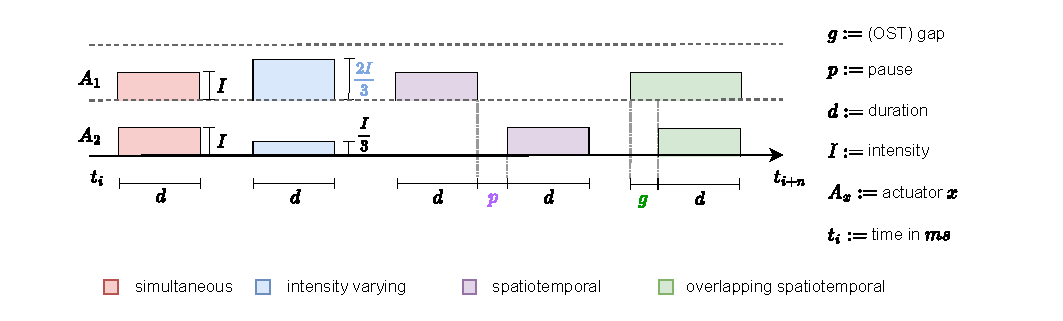
\includegraphics[width=\linewidth]{src//pictures/ost_diagram.drawio.pdf}
    \caption{Chord encoding schemes used in previous literature \cite{Luzhnica2017,Luzhnica2016,Luzhnica2018,Luzhnica2018a}.}
    \label{fig:chord_encoding}
\end{figure}

One of the primary challenges associated with Braille typing in the context of passive learning is the chorded input aspect. This refers to the simultaneous pressing of multiple keys or buttons to generate a single character, which can be particularly demanding in a passive learning environment. Chorded input often requires a high degree of motor coordination and precision, posing unique challenges for learners who lack active engagement during the learning process.

The encoding and execution of chords—actions involving the simultaneous use of multiple limbs or fingers—are central to many real-world tasks, such as playing musical instruments like the piano \cite{Seim2014, Seim2015b, Huang2008, Kohlsdorf2010, Huang2010, Seim2014a, Vaio6810, Donchev2021, Fang2023a, Fang2023}, performing multi-limb rhythms on drums \cite{Bouwer2011, Holland2010}, and Braille writing itself \cite{Learning2024, Seim2017, Seim2014a}. These activities demand the integration of complex motor skills, making them particularly challenging to teach through passive learning. As such, developing effective methods to teach users how to perform chords is crucial.

Several approaches have been explored to encode and teach chorded inputs, as illustrated in Fig. \autoref{fig:chord_encoding}. Seim et al. identified that encoding chords is especially challenging due to the difficulty participants face in accurately distinguishing simultaneous stimuli of multiple fingers, a problem depicted in red in Fig. \autoref{fig:chord_encoding} \cite{Seim2014, Seim2015}. 

In an attempt to address these challenges, Luzhnica et al. investigated the use of varying stimulus intensities (depicted in blue in Fig. \autoref{fig:chord_encoding}) to differentiate between inputs. However, this approach proved to be ineffective, as the variation in intensity did not provide sufficient clarity for learners to distinguish between stimuli \cite{Luzhnica2017}.

A more promising method, proposed by Seim et al., involves staggered input, where stimuli are activated or deactivated sequentially rather than simultaneously (depicted in purple in Fig. \autoref{fig:chord_encoding}). This spatiotemporal encoding method, first introduced by Seim et al. \cite{Seim2014a} and adopted in subsequent studies \cite{Seim2014}, enables a clearer temporal distinction between stimuli. By presenting stimuli sequentially, learners are better able to recognize and understand chord patterns, improving learning outcomes. However, this approach has limitations, particularly with encoding speed. The sequential nature of the method can slow down the process, especially for complex chords, thereby impacting overall learning efficiency.

To overcome these speed limitations, Luzhnica et al. introduced the \gls{ost} encoding method, depicted in green in Fig. \autoref{fig:chord_encoding}. This method improves upon the spatiotemporal approach by overlapping the activation of actuators. Specifically, one actuator is turned on, followed by a delay (the OST-gap $g$) before activating the next, with all actuators remaining active for a fixed duration $d$ before being turned off simultaneously. The \gls{ost} method not only enhances encoding speed but also ensures that patterns are maintained longer, improving both accuracy and the overall learning experience \cite{Luzhnica2018, Luzhnica2018a, Luzhnica2017, Luzhnica2016}.

Further refinements to the \gls{ost} encoding method were explored in a follow-up study by Luzhnica et al. \cite{Luzhnica2017}. They found that prioritizing more sensitive areas of the skin during the \gls{ost} encoding process improved accuracy while increasing the delay between activations had little impact on performance. These findings highlight the robustness and effectiveness of the \gls{ost} method in addressing the challenges of chorded input in passive learning \cite{Luzhnica2017}.


\section{Braille Learning}
\begin{figure}
    \centering
    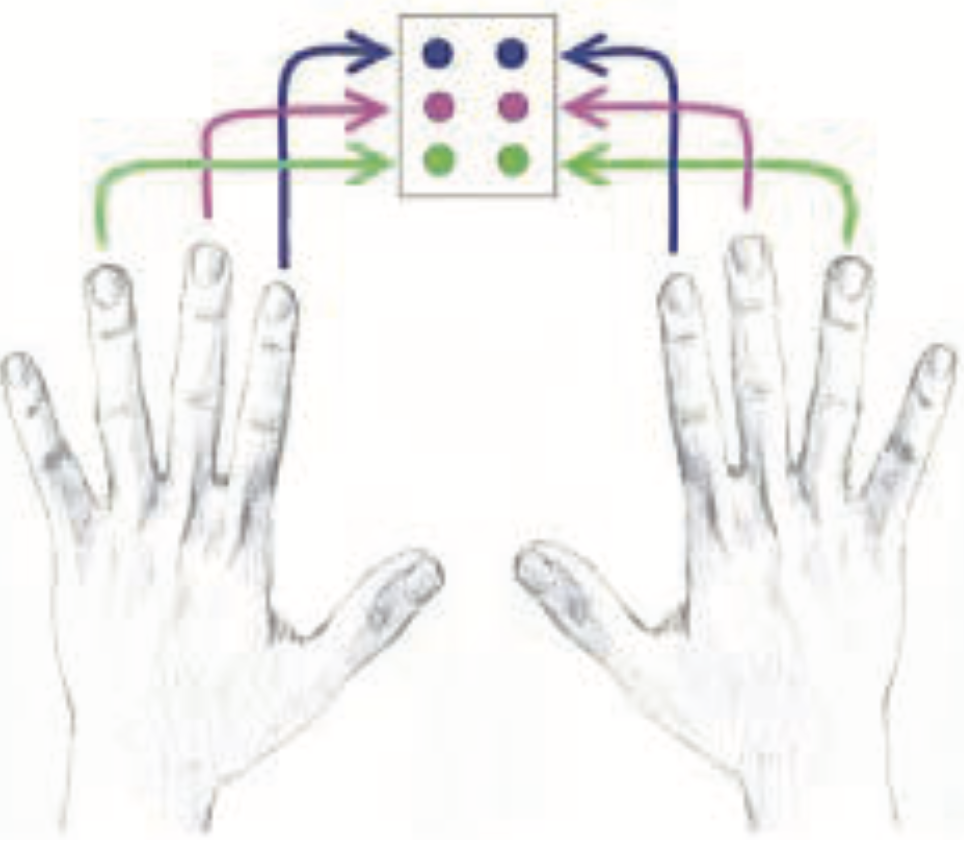
\includegraphics[width=0.5\linewidth]{src//pictures/Screenshot 2024-09-12 at 20.13.38.png}
    \caption{Braille finger mapping \cite{Seim2014a}.}
    \label{fig:braille-key-mapping}
\end{figure}
\begin{figure}
    \centering
    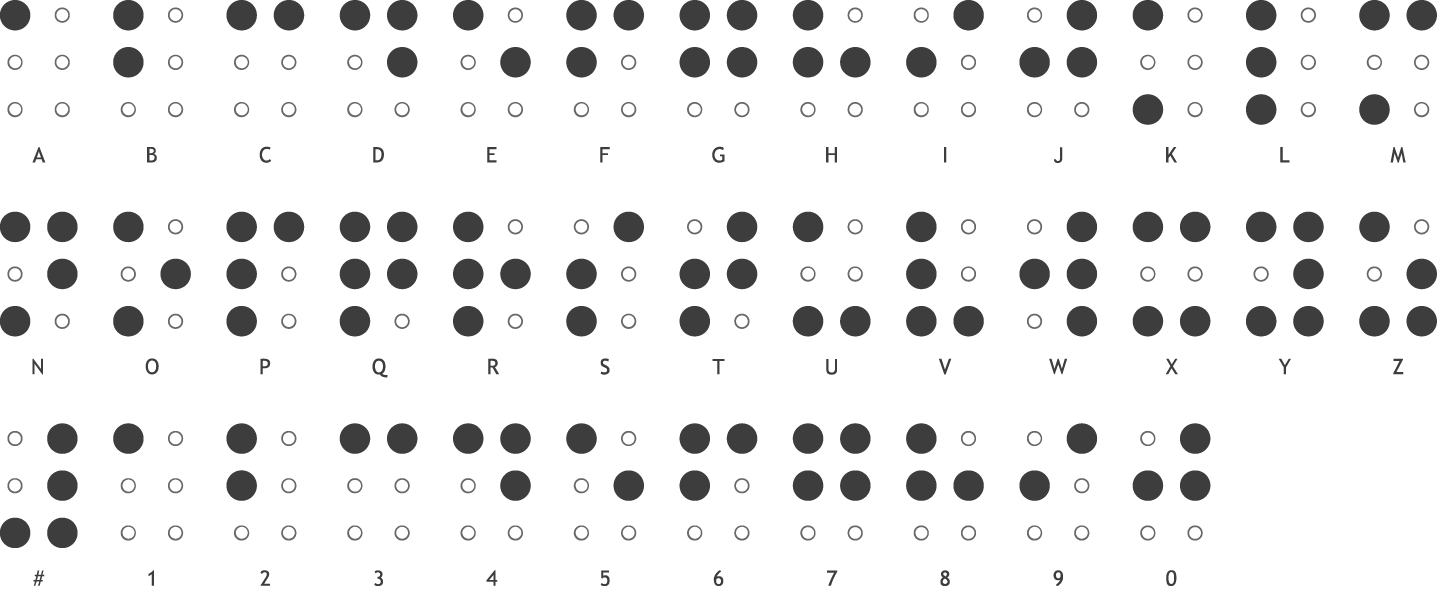
\includegraphics[width=0.5\linewidth]{src//pictures/braille_alphabet.png}
    \caption{English Braille alphabet (Grade One) \cite{pharmabrailleBrailleAlphabet,troughton1992guidelines}.}
    \label{fig:braille-alphabet}
\end{figure}
Braille, a tactile writing system, was developed in 1825 by Louis Braille\footnote{\url{https://www.dbsv.org/wie-die-brailleschrift-funktioniert.html}}. It is composed of a six-dot system, as illustrated in Fig. \autoref{fig:braille-alphabet}, which allows users to type characters by pressing combinations of six keys simultaneously, as shown in Fig. \autoref{fig:braille-key-mapping}. Devices like the Perkins Brailler, the most commonly used Braille typewriter, facilitate this process. The Perkins Brailler consists of six main keys for typing, along with a space bar and secondary keys \cite{Wikipedia2023}. Despite its utility, teaching and learning Braille remains one of the most significant challenges, particularly due to the time-intensive nature of mastering the system.

The integration of technology in Braille education has gained traction but remains underutilized, especially for senior learners. A 2018 study by Martiniello et al. \cite{Martiniello2018} found that while 62.5\% of \gls{tvi} and Rehabilitation Specialists working with younger learners use technology in their instruction, only 26.3\% do so with seniors. Rehabilitation Specialists were also found to use technology less frequently than \gls{tvi}, though \gls{tvi} reported that technological tools enhance learner motivation and improve outcomes. Among these tools, the Braille Tutor app stands out. Available on multiple platforms, it has been downloaded over 100,000\footnote{\url{https://play.google.com/store/apps/details?id=com.lukeneedham.brailletutor&hl=en}\\and \url{https://brailliac.com/}} times. McCarthy et al. \cite{McCarthy2016} demonstrated that the app increased students’ learning rates, allowing them to achieve 100\% accuracy faster and learn more Braille contractions—a shortened form of Braille words, also called Grade two Braille\cite{troughton1992guidelines}.

In addition to digital methods, non-digital programs such as the Mangold Braille Program \cite{Mangoldnd} and resources from Hadley\footnote{\url{https://hadleyhelps.org/learn?topic_id=15}} play a vital role.
The Mangold Program focuses on tactile perception and symbol recognition before introducing the Braille alphabet through 29 progressive lessons. Hadley, endorsed by the New York State Commission for the Blind (NYSCB)\footnote{https://ocfs.ny.gov/programs/nyscb/assets/docs/BrailleFAQ.pdf}, offers self-learning resources but emphasizes that learning Braille, particularly contracted Braille, is a lengthy process, often requiring over a year. Tools like Alpha Boxes\footnote{https://www.pathstoliteracy.org/alpha-boxes/}, which pair initial letter sounds with Braille symbols, provide additional support for early learners.

Despite these resources, one-to-one teaching between students and teachers remains the dominant method for Braille instruction, as noted by Jawasreh et al. \cite{Jawasreh2020}, who developed the Braille Finger Puller, a haptic device aimed at innovating the teaching process. Similarly, haptic technologies, such as the Translation Glove by Subathra et al. \cite{Subathra2024}, have been designed to use vibrations to support Braille learning, akin to the gloves developed by Bandodkar et al. \cite{Bandodkar2014} and Shivakumarl et al. \cite{Shivakumarl2013}. However, most devices rely on vibration gloves, with few exploring \gls{phl}. Like Seim et al. and Caulfield et al., \cite{Learning2024} have investigated this technique, though it remains underutilized in existing Braille learning devices. Furthermore, none of the current technologies incorporate \gls{ost} encoding, a method with significant potential to improve tactile learning efficiency.

Studies have also explored Braille learning among sighted individuals. Bola et al. \cite{Bola2016} conducted a nine-month study with 29 sighted adults, mostly Braille teachers, and found that participants could read Braille at an average speed of six words per minute by the course’s end. Interestingly, low tactile accuracy did not significantly affect reading speed, indicating that even sighted individuals can adapt their sensorimotor systems to Braille without visual deprivation. Their learning rate was comparable to congenitally or early blind children learning Braille in primary school. Some educators have even employed methods like blindfolding children with residual vision to accelerate their tactile learning \cite{Bola2016}.

Additional research has focused on variables influencing Braille learning rates. Hall et al. \cite{Hall1987} identified study modality (visual or haptic), stimulus discriminability, and test modality as key factors affecting performance during the learning phase. These insights have informed the development of teaching strategies and tools to better accommodate diverse learners.

Despite advancements, learning Braille remains a slow and challenging process, often requiring months or even years to achieve proficiency, particularly in contracted Braille. This underscores the need for further innovation in teaching methods and devices, particularly those incorporating \gls{phl} and \gls{ost} encoding, to enhance the efficiency and accessibility of Braille instruction.




    %12
% \section{Related Works}
\subsection{Piano Learning}
In 2008, Huang et al. \cite{Huang2008} investigated the effectiveness of learning piano through passive haptic feedback combined with audio cues. A study was conducted utilizing a specialized glove embedded with vibration motors corresponding to each finger, designed to assess whether passive exposure to a combination of auditory and tactile stimuli could improve piano learning and performance relative to learning through auditory stimuli alone. Participants wore the glove while engaging in a 30-minute distraction task, such as reading or typing, during which piano music was played and corresponding finger vibrations were delivered. Afterwards, they were asked to play the piano pieces they had been exposed to. The results revealed that participants who received both audio and haptic feedback performed significantly better, playing the pieces more smoothly and with fewer errors compared to those who received only audio feedback. The latter group exhibited more hesitation and confusion. The study concluded that \gls{phl} can significantly enhance piano skill acquisition by reducing errors and improving performance fluidity. The combination of audio and tactile feedback provided a richer understanding of the musical structure, reinforcing the potential of \gls{phl} as a valuable tool for learning physical skills, such as piano playing.

Further investigation into this phenomenon was conducted within the \gls{mmt} framework. The first work by \cite{Huang2010} explored the potential of using \gls{phl} to teach piano playing, focusing on whether individuals could learn piano passages through haptic feedback delivered via fingerless vibration gloves and how this method compared to traditional active learning methods.
Two studies were conducted. In the first study, novice participants were asked to learn and reproduce a musical passage after a 30-minute session of \gls{phl} using the \gls{mmt}  system. During the session, participants engaged in a reading comprehension task while receiving tactile cues via the gloves. The results showed that participants who received tactile stimulation performed better than those in the control group, demonstrating that \gls{phl} can effectively teach piano passages. Interestingly, participants without prior musical experience tended to perform better with \gls{phl} than those with musical backgrounds. In the second study, the researchers compared the time required to learn a short, randomly generated musical passage using either passive or active learning methods. Participants with no prior piano experience often succeeded in repeating the passage correctly after \gls{phl}, while those with musical experience found the process more challenging. This study highlighted the advantages of \gls{phl} for novices, as it required fewer attempts to learn the passage compared to active learning, particularly for those without a musical background.
The paper also found that while audio alone was insufficient for effective learning, the combination of tactile feedback and passive exposure to musical sequences significantly improved participants' ability to learn and reproduce the music.

The second \gls{mmt} paper reported by \cite{Kohlsdorf2010} examined the impact of different primary tasks on the effectiveness of \gls{phl} in teaching piano note sequences. Three primary tasks were examined while participants received passive haptic feedback to learn a random 10-note piano sequence: watching a film (audio-visual stimulation), playing a memory game (active memory engagement), and walking a designated path (body motion). These tasks represented common everyday activities like relaxing, thinking, and walking. Participants initially observed and listened to the piano keyboard as it played a 10-note sequence, after which they attempted to replicate the sequence. If they were unable to do so successfully, they proceeded to engage in the primary task for five minutes while receiving targeted finger stimulation via the \gls{phl} device. Following this stimulation, participants made another attempt to reproduce the sequence. This cycle was repeated until the participant was able to accurately replicate the sequence with 100\% accuracy. The results indicated no statistically significant difference in the number of \gls{phl} sessions required across the different primary tasks. However, individual differences were noted, with some participants finding certain tasks more challenging than others. Rhythm retention was slightly better after the memory game condition compared to the film condition, though no condition was significantly better or worse overall. Participants reported similar subjective workloads across all conditions, suggesting that the type of primary task does not significantly impact the effectiveness of \gls{phl} in learning piano sequences. The study concluded that while the type of primary task may influence individual performance, there is no clear evidence that one task is superior to others for \gls{phl} effectiveness. This suggested that \gls{phl} can be effectively integrated into various everyday activities without being significantly hindered by the nature of the concurrent task.

Based on the aforementioned results, \cite{Seim2015b} investigated the potential of using \gls{phl} to teach two-handed, chorded piano melodies, focusing on the effectiveness of \gls{phl} in teaching complex motor skills and the necessity of accompanying audio feedback. The study introduced a method of sequentially delivering tactile stimulation to each finger involved in a chord, rather than simultaneous stimulation which has been proven to be ineffective, to facilitate the learning of complex piano pieces\cite{Luzhnica2017, Luzhnica2016, Luzhnica2018, Luzhnica2018a, Seim2014a}.
The study comprised two experiments. In the first, participants were exposed to vibration-only and vibration-plus-audio conditions while learning a simple one-handed piano melody. Their performance, assessed using Dynamic Time Warping (DTW), indicated no significant difference between the two conditions, suggesting audio feedback was not essential for effective learning with \gls{phl}.
In the second experiment, participants without prior piano experience were randomly assigned to one of the following four conditions: no feedback; audio only; vibration only; and audio with vibration. Those in the vibration-only and vibration-plus-audio groups performed significantly better than the control and audio-only groups, indicating the effectiveness of tactile feedback in learning motor skills. However, participants reported higher frustration levels when audio was combined with vibration, as measured by the NASA Task Load Index (NASA TLX).
The study concluded that \gls{phl} is effective for teaching two-handed, chorded piano melodies, particularly with tactile feedback alone. These findings suggest that passive haptic stimulation can suffice for learning motor skills, even with minimal attention dedicated to the task. The research also has broader implications for teaching other complex motor skills, like Braille typing, through \gls{phl}, and reinforced that \gls{phl} is most effective when teaching sets of 10-17 stimuli at a time, as explored in previous work \cite{Seim2014a}.

In $2021$, Donchev et al. \cite{Donchev2021} explored the effectiveness of \gls{phl} in teaching and retaining piano note sequences, comparing it to active learning methods. The study aimed to determine whether \gls{phl} could be as effective as active learning for memorizing and recalling piano sequences and to assess the long-term retention of these sequences.
Participants were taught a 10-note piano sequence through both active and \gls{phl} methods and were then tested three days later to evaluate their retention of taught sequences. The study design was based on previous \gls{phl} research, particularly the \gls{mmt} tactile stimulation method, but with modifications to prevent overlearning, as participants were stopped once they achieved 90\% accuracy during the learning phase.
The results indicated no significant difference in unaided recall between actively and passively learned note sequences when participants were asked to play from memory. However, when provided with auditory and visual cues, participants were significantly better at recalling the passively learned sequences. This suggested that while both learning methods are effective, \gls{phl} may offer advantages in cued recall situations. The study also observed a recency effect in \gls{phl}, where more recently learned material was better retained.
Moreover, the study found that while \gls{phl} took longer initially, participants required fewer attempts to learn the sequences and demonstrated a 10\% higher retention rate compared to active learning. This suggested that \gls{phl} can be a highly effective method for teaching and retaining complex skills like piano playing, especially when cues are provided during recall.

In $2023$, \ea{Fang}{\cite{Fang2023a}} investigated the impact of \gls{phl} on rhythm learning across different musical instruments, focusing on the keyboard and ukulele. The study also examined whether combining haptic feedback with audio enhances rhythm learning, as measured by accuracy in duration and timing.
Participants were divided into three groups: one receiving haptic feedback only, another receiving both haptic and audio feedback, and a third receiving audio feedback only. Inspired by previous research on \gls{phl} in piano learning\cite{Donchev2021, Huang2010}, the study offset the haptic and auditory signals by a few seconds to avoid overlap. The results indicated that the effectiveness of learning varied depending on the feedback method and the instrument used. For rhythm duration accuracy, the group that received only haptic feedback performed the best on the keyboard, followed by the group that received both haptic and audio feedback. However, performance across all groups was notably poor on the ukulele, suggesting that haptic feedback alone may be insufficient for learning more complex instruments.
Regarding timing accuracy, rhythms played on the keyboard were generally reproduced more accurately, with the group receiving both haptic and audio feedback achieving near-perfect timing. In contrast, the group relying solely on haptic feedback demonstrated the greatest difficulty with timing accuracy, particularly on the ukulele. Interviews with participants further revealed that the combination of haptic and audio feedback was advantageous for rhythm learning, especially when using the keyboard. However, relying exclusively on haptic feedback was found to be the least effective approach, particularly when applied to more complex instruments like the ukulele. The study concluded that while \gls{phl} can be effective for rhythm learning, its efficacy is contingent upon the instrument used and the type of feedback provided. The combination of haptic and auditory feedback consistently produced the most favourable outcomes, particularly in terms of timing and duration accuracy. Conversely, haptic feedback alone was insufficient for more complex instruments, such as the ukulele, resulting in the least successful learning outcomes. These findings indicate that integrating both haptic and auditory feedback is crucial for achieving optimal rhythm learning across various instruments.

Following these results, \cite{Fang2023} investigated whether other kinds of stimuli apart from vibration might be beneficial for \gls{phl}, exploring the effectiveness of different tactile sensations in \gls{phl} for piano songs. The study aimed to determine whether affective tactile sensations are as effective as the more commonly used discriminative sensation of vibration in teaching motor tasks through \gls{phl}. Additionally, it examined whether there are differences in learning rates and user perceptions across these tactile modalities. Each participant learned three different note sequences using the three tactile systems (vibration, tapping, and stroking) in a within-study design. After a 30-minute \gls{phl} session for each system, participants were tested on their ability to recall and play the sequences. The results indicated no significant differences in the effectiveness of the three tactile systems for \gls{phl}, confirming that all three modalities—vibration, tapping, and stroking—are effective for teaching piano sequences. However, tapping and stroking were found to be slightly more effective than vibration, with participants learning more notes and making fewer errors (up to $1.06$ fewer errors on average) when using these affective sensations. Additionally, over $50\%$ of participants rated stroking as the most pleasant sensation, while only $11\%$ favoured vibration. The study also highlighted that \gls{phl} is particularly beneficial for inexperienced users, consistent with previous research. However, the overall accuracy rate per note sequence was lower than in earlier studies, possibly due to the absence of recall aids during the testing phase, such as auditory or visual cues.


\subsection{Typing Skills}
Building on the success of \gls{phl} in the \gls{mmt} project \cite{Markow2010, Kohlsdorf2010, Huang2010}, Seim et al. extended their research to explore its application in typing systems, aiming to use these findings as a foundation for passively teaching Braille typing \cite{Seim2014}. They investigated whether complex skills, such as typing and chord recognition, could be effectively taught through tactile interfaces using \gls{phl}, and also examined the role of visual feedback in the learning process.
Participants in the study were taught typing skills using fingerless gloves embedded with vibration motors. During practice sessions, audio cues were followed by corresponding vibration patterns to stimulate finger presses. Participants then typed the patterns into software that displayed either the actual letters they typed or asterisks as feedback. The study aimed to determine whether visualizing the letters during typing would aid or impede learning.
The results showed that visual feedback, where participants saw the letters they typed, actually hindered their performance compared to using asterisks or vibration only. Those using vibration-only feedback achieved better accuracy, though their typing speed was lower. This suggested that visual prompts may not be effective for \gls{phl}-based typing and that users might benefit more from audio prompts.
The study also found that the random presentation of letters and words did not significantly impact learning, highlighting the importance of session length and information chunk size. However, teaching chords through \gls{phl} was unsuccessful, as participants had difficulty distinguishing which fingers were being stimulated. The researchers concluded that accuracy, rather than speed, should be the primary metric for evaluating \gls{phl} effectiveness.
In a follow-up experiment, a \gls{phl} session without active practice was conducted, where participants played a memory card game while receiving training. The results indicated that participants could type with a low error rate and maintain consistent performance, successfully learning to use both hands with \gls{phl}. Some even achieved perfect accuracy on new phrases, though at reduced typing speed. This suggested that \gls{phl} can effectively teach typing skills, including the mapping of letters to keys.
Overall, the study concluded that \gls{phl} is a valuable method for teaching typing skills, particularly when using audio prompts rather than visual feedback. However, its effectiveness in teaching more complex tasks, such as chord recognition, remains limited.

To further investigate the potential of \gls{phl}, Seim expanded their research to determine whether it could be applied to a multi-row keyboard rather than the traditional one-finger-to-one-key mapping \cite{Seim2017}. The study focused on enhancing the speed and accuracy of a motor task, specifically numeric entry on a randomized keypad. The aim was to assess whether \gls{phl} could improve typing speed and reduce reliance on visual cues in a text entry system.
The researchers conducted a study using a 4x3 numeric keypad with a randomized key mapping, designed for use with the right hand only. The study included a pretest to establish a baseline, followed by multiple sessions in which participants alternated between a distraction task and a typing test. During the distraction task, participants in the \gls{phl} group received passive tactile stimuli corresponding to one row of the keypad at a time, which facilitated chunking and improved spatial memory.
The results demonstrated that participants in the \gls{phl} group significantly improved their typing speed compared to the control group. Additionally, \gls{phl} users looked at the keyboard significantly less during the task, indicating improved familiarity with the key layout and reduced dependency on visual cues. This suggested that \gls{phl} can effectively convert tactile stimuli into motor movements and enhance performance in text entry systems.
A pilot study included an additional test where participants’ hands were covered by a paper screen to assess their knowledge of the keypad layout without visual assistance. This further confirmed the effectiveness of \gls{phl} in reinforcing the spatial memory needed for typing.
The study concludes that \gls{phl} can be a powerful tool for improving motor task performance, particularly in learning and mastering keyboard typing skills. The use of wearable computing devices that provide passive tactile feedback presents a promising solution for training and enhancing the speed and accuracy of text entry tasks.

\subsection{Braille Learning}

Building on the initial success with typing, Seim et al. \cite{Seim2014a} explored the effectiveness of \gls{phl} in teaching Braille typing and reading through wearable technology. The study aimed to determine whether \gls{phl} could reduce errors in Braille typing and enhance the recognition and reading of Braille letters compared to traditional learning methods.
Participants in the study were passively taught the full Braille alphabet over several sessions using a wearable device that provided haptic feedback. The instruction method utilized a chorded input system based on sequential tapping patterns, a technique that had previously been ineffective with non-sequential patterns \cite{Seim2014a}. Participants engaged in tactile and visual Braille letter identification tasks, along with a distraction task to rigorously assess their learning.
The results demonstrated that participants who received passive haptic instruction exhibited a significant reduction in typing errors when typing phrases in Braille compared to those who did not receive haptic feedback. Moreover, participants were able to recognize and read more Braille letters from the phrases they typed, achieving a high recognition rate of the entire Braille alphabet by the end of the study. These findings suggested that \gls{phl}, facilitated by wearable technology, is a feasible and effective method for teaching Braille typing and reading.
The study also revealed that \gls{phl} allowed participants to learn words and complete their learning more quickly than those who did not receive haptic feedback. This indicates that typing practice in this context may also serve as effective reading practice, further enhancing the learning experience. The researchers concluded that \gls{phl} could be a valuable tool in Braille education, offering a passive yet powerful means of learning complex text entry skills.

Following this success, Caulfield et al. \cite{Learning2024} investigated the impact of a \gls{phl} glove on the learning rate, proficiency, and recall rate in Braille learners. The study compared the effectiveness of the glove-based \gls{phl} method with traditional memorization approaches.
The study was conducted in three phases. In the first phase, participants used flashcards to associate letters with Braille cell orientations, serving as a baseline for evaluating their initial proficiency without haptic feedback. The second phase involved a typing exercise using a keyboard, with some participants receiving haptic feedback through the glove while typing. The third phase consisted of a recall test conducted both with and without haptic feedback, followed by a retention test conducted several days later.
The results indicated no statistically significant difference in the effectiveness of using \gls{phl} via the glove compared to traditional memorization methods. While the glove provided haptic feedback, it did not significantly enhance learning outcomes. In some cases, the glove even appeared to hinder performance, as suggested by longer response times and lower recall rates in participants who used the glove. The study concludes that the \gls{phl} system tested may not be an effective tool for improving Braille learning.

\subsection{Morse Code}

In $2016$, Seim et al. investigated whether \gls{phl} could teach rhythm by using Google Glass to passively teach Morse code through head-based vibrations \cite{Seim2016a}. The study focused on whether Morse code, a rhythm-based system, could be learned passively through vibrations on the head rather than through hands, which are typically used in haptic feedback studies.
Participants were randomly assigned to either a control group or a \gls{phl} group. The \gls{phl} group received rhythmic haptic feedback via Google Glass's \gls{bct} while learning Morse code, while the control group only heard the words without Morse code information. Over four hours, participants engaged in various learning and distraction tasks, including typing and perception tests, to assess their Morse code proficiency.
The results showed that \gls{phl} could effectively teach Morse code using head-based vibrations. The \gls{phl} group achieved 94\% accuracy on a pangram typing task, with most participants reaching 100\% accuracy by the end of the study. They were also able to recognize and reproduce Morse code rhythms with minimal errors, demonstrating that the rhythm-based nature of Morse code could be learned through head-based haptic feedback. The \gls{phl} group outperformed the control group, showing a lower error rate and increased typing speed, which improved from $2.5$ words per minute (WPM) to $4$ WPM, approaching the target speed of $10$ WPM.
The study concluded that \gls{phl} is a viable method for teaching rhythm-based non-motor skills like Morse code through \gls{bct} devices like Google Glass. It highlighted the potential of \gls{phl} for eyes-free, silent text entry on mobile devices, offering new possibilities for learning and communication. However, it also noted that some active learning might occur when visual feedback is provided during testing, suggesting that future research should further isolate and measure the effects of \gls{phl} alone.

After the success, Seim et al. explored in \cite{Seim2018} the potential of using smartwatch haptics to facilitate \gls{phl} of new skills, specifically focusing on Morse code. The study aimed to determine whether the subtle haptic feedback typically used for message alerts on smartwatches is sufficient for teaching skills and to compare the effectiveness of different durations of passive stimulation.
The researchers conducted a study where participants used a smartwatch to deliver low-amplitude haptic stimuli corresponding to Morse code. Participants underwent a pre-test to assess their initial knowledge of Morse code, followed by a period of \gls{phl} where they received haptic feedback while engaged in a distraction task. The study was designed as a between-subject experiment, with participants split into two groups: one receiving 8 minutes of passive stimulation per word and the other receiving 16 minutes.
The results demonstrated significant improvements in participants' ability to recall and recognize Morse code from pre-test to post-test, with those in the 16-minute stimulation group showing a 25-75\% improvement in accuracy compared to the 8-minute group. This suggested that extended exposure to haptic feedback enhances learning outcomes. A follow-up recall test administered 1-3 days later indicated that the participants retained the information learned during the study.
The study concludes that smartwatches, despite their low-amplitude actuators, can effectively support \gls{phl} and help users learn new skills like Morse code. The findings suggested that longer durations of haptic stimulation may lead to better retention and performance, indicating that smartwatch haptics could be a viable tool for skill acquisition through \gls{phl}. This research opened up new possibilities for using everyday wearable devices for educational and training purposes.

However, \cite{Pescara2019} suggested that the training and testing procedures used in earlier studies may have leaked information to participants, leading to inadvertent active learning. They revisited and critiqued the design choices of previous studies such as \cite{Seim2016a, Seim2018}, highlighting potential flaws that might have facilitated active learning \cite{Pescara2019}.
To address this, \cite{Pescara2019} investigated whether \gls{phl} could effectively teach Morse code without requiring active attention from learners, building on prior research. The study divided participants into five groups to explore the effectiveness of \gls{phl} in teaching Morse code. Participants were exposed to vibration patterns on a wristband, each corresponding to a Morse code character, while also engaging in distraction tasks of varying difficulty to simulate divided attention.
The results showed that while it is possible to learn Morse code passively through haptic feedback, learning rates were significantly lower compared to when active attention was involved. The findings suggested that \gls{phl} can facilitate the acquisition of simple motor skills with minimal attention but is less effective for complex, non-motor tasks like learning Morse code, which requires declarative memory engagement. The study also found that participants performed better when feedback was provided during learning, though the difficulty level of the distraction tasks did not significantly affect outcomes.

\subsection{Multi-limb Rhythm Learning}
In $2011$, the potential of \gls{phl} for multi-limb skills was further explored. Bouwer et al. \cite{Bouwer2011} introduced the Haptic Ipot \cite{Holland2010, Bouwer2011}, a system designed to teach drumming techniques. In this study, participants wore elastic Velcro bands equipped with haptic vibrotactile devices that delivered rhythmic stimuli to different limbs. The stimuli were played back silently, and during the haptic feedback sessions, participants engaged in a reading comprehension task, similar to those used in previous studies \cite{Huang2008, Huang2010}.
Participants were exposed to two different rhythms, and their baseline performance was measured using a MIDI drum kit. Following the \gls{phl} session, participants were tested again on the MIDI drum kit to evaluate their accuracy, timing, number of attempts, and errors during their best attempt. A questionnaire was also administered to collect subjective feedback on the learning experience.
The preliminary results suggested that \gls{phl} of multi-limb rhythms is a promising approach. Participants demonstrated improvements in both rhythm accuracy and timing, indicating that even while focusing on other tasks, individuals can still absorb and reproduce complex rhythmic patterns through haptic feedback.


\subsection{Skin Reading}

\Gls{vsr} \cite{Luzhnica2016} is a method of encoding vibrotactile patterns to represent symbols, which can be combined to convey complex messages such as words and phrases \cite{Luzhnica2018}. Building on their previous research on VSR, Luzhnica et al. \cite{Luzhnica2018} explored the effectiveness of \gls{phl} as a training method for skin reading, where information is conveyed through vibrotactile patterns. This study specifically investigated whether \gls{phl} can be used to teach participants to comprehend text transmitted via these patterns and examines whether the speed of transmission affects recognition accuracy.
The researchers conducted an experiment in which participants underwent 30 minutes of training to learn 10 letters of the German alphabet encoded into vibrotactile patterns. The training utilized a glove with six vibromotors placed on the back of the hand, replicating the design from \cite{Luzhnica2016}. Each letter was encoded by activating one or two vibromotors in an \gls{ost} sequence, which is known to provide better perception than the simultaneous activation of multiple motors.
During the training, participants engaged in a distraction task, such as playing a game\footnote{The snake game \url{https://en.wikipedia.org/wiki/Snake_(video_game_genre)}}, while passively receiving vibrotactile cues. Each letter's pattern was repeated multiple times over 12 rounds of training. In addition to the pre-and post-tests, the study conducted a recall test the following day to assess the participants' ability to reconstruct and recognize the letters they had learned \cite{Luzhnica2018}.
The results demonstrated that participants could recall the learned vibrotactile patterns and accurately reconstruct and recognize the letters immediately after training and one day later. The accuracy of recognition and reconstruction was consistent with previous research, indicating that \gls{phl} is an effective method for training skin reading. Additionally, the study found no significant difference in comprehension accuracy across different transmission speeds, suggesting that participants could accurately comprehend the information transmitted at varying speeds.
And, henceforth, concludes that \gls{phl} is a promising and effective method for training vibrotactile skin reading, offering a viable alternative to more demanding and time-consuming active training methods. The ability to comprehend information regardless of transmission speed further enhances the potential applications of \gls{phl} in this domain.


\subsection{Effects of PHL Practice in Rehabilitation}
In their work on the \gls{mmt} framework in $2010$, Markow et al. explored potential improvements in dexterity and sensation for patients with incomplete \gls{sci} while learning a new skill set. This research led to their second \gls{mmt} paper \cite{Markow2010}, which presented a pilot study on hand rehabilitation in individuals with tetraplegia due to \gls{sci}.
The study demonstrated that \gls{mmt} could stimulate afferent nerves, potentially improving motor function and sensory perception through the active learning (piano practice) mode. Participants with tetraplegia indicated progress in sensory tests such as the Semmes-Weinstein monofilament evaluation and the Grasp and Release Test (GRT) after four weeks of practice, consisting of three 30-minute sessions per week. Additionally, three different glove designs were tested: a golf-style glove, an open-flap glove, and a Velcro-finger glove (as depicted in \autoref{fig:glove_designs}).
The preliminary findings suggested that \gls{mmt} holds promise as a hand rehabilitation for individuals with tetraplegia resulting from incomplete \gls{sci}. The work presented in this paper lays the foundation for future studies to evaluate the broader applicability of \gls{mmt} in the tetraplegia population.

\subsection{Stenography Learning}

Aveni et al. \cite{Aveni2019} explored passive haptic learning (\gls{phl}) for stenography training, focusing on a system that combines tactile feedback with spatial tasks. The study aimed to teach participants to use a stenotype keyboard, where each key corresponds to an English sound. Over four 10-minute sessions, participants wore two-handed fingerless gloves with a vibration motor on the dorsal side of each hand and played the game "SpikeDislike2" as a distraction\footnote{\url{https://gamejolt.com/games/spikedislike2/}}.
The training focused on combining “subchords,” or word-parts, to form unfamiliar words. Each finger was responsible for two keys, except the left pinky, and the system used temporal offsets in the vibration patterns to stimulate the fingers from left to right and top to bottom. A distinct tapping rhythm indicated whether the top, bottom, or both keys needed to be pressed simultaneously.
Results showed a significant improvement in typing accuracy compared to the control group, based on uncorrected error rates.
The study demonstrated that passive tactile feedback can help novices learn stenography, even without explicit instruction on combining subchords. Participants autonomously figured out word formation through the modular training structure, with errors mainly being horizontal or vertical, indicating correct finger placement. This suggests \gls{phl} as an effective and intuitive method for teaching complex skills like stenography.  %9.  ->22


%  \chapter{Implementation of your Project}
\label{ch:Implementation}

\section{Design}
This section presents the design and the key design decisions we made for this project.
We begin by describing the hardware apparatus, which includes the actuators and the gloves themselves, as well as the design iterations undertaken during the development of the glove.
Next, we outline the software components, detailing the encoding of the actuators, the communication protocol, and providing a brief introduction to the associated software elements.
Finally, we conclude this section by introducing the study design of the two studies conducted to address our research questions.


\subsection{Hardware}
We have divided this subsection into two parts: the first focuses on the actuators used, while the second discusses the design of the Velcro gloves.

\subsubsection{Actuator Design}
For the actuators and their setup, we adopted the design and configuration proposed by Fang et al. \cite{Fang2023}, using Velcro straps. This decision was informed by prior research \cite{Markow2010, Kohlsdorf2010, Huang2010, Fang2023a}, which highlights the importance of design factors such as weight, breathability, flexibility, and coarseness for user comfort, particularly during extended wear. Velcro straps effectively meet these criteria while enhancing dexterity, a recognized advantage of fingerless glove designs \cite{Huang2008}. This design facilitates everyday tasks and accommodates a range of finger sizes, making the gloves adaptable for different users. Furthermore, using the same actuators enables a direct comparison with Fang et al.’s prior work \cite{Fang2023}, which employed identical actuators in a one-handed, non-chorded piano learning setup.

The actuators consist of six vibration systems (three per hand), with one shown in \autoref{fig:fang-vibration}. Each system includes a vibration motor (Brand: Grove Seed; Model: ANDA-B1020) housed in a 3D-printed PLA case and secured with Velcro bands. Operating at a frequency of approximately 200 Hz, the vibration motors are directly connected to the glove for control. Each system is mounted in a curved-bottom 3D-printed case for optimal fit, as illustrated in \autoref{fig:fang-vibration}, where it is demonstrated on a single finger. Consistent with Fang et al.’s design \cite{Fang2023}, larger contact areas were used to allow easier adjustment for individual comfort. The actuators operate at an amplitude of 1.03 G and weigh 6.6 grams each.

\begin{figure}
     \centering
     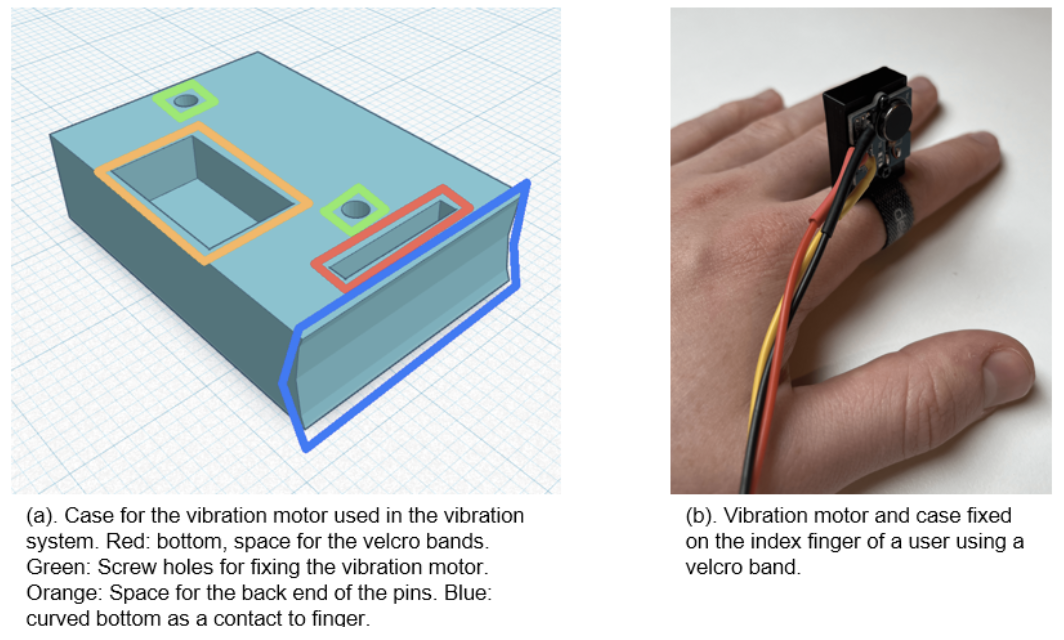
\includegraphics[width=0.5\linewidth]{src/pictures/Screenshot 2024-09-12 at 15.11.57.png}
     \caption{3D model, and the implementation on a users finger of one element of the vibration system from \cite{Fang2023}}
     \label{fig:fang-vibration}
 \end{figure}
\begin{figure}
    \centering
    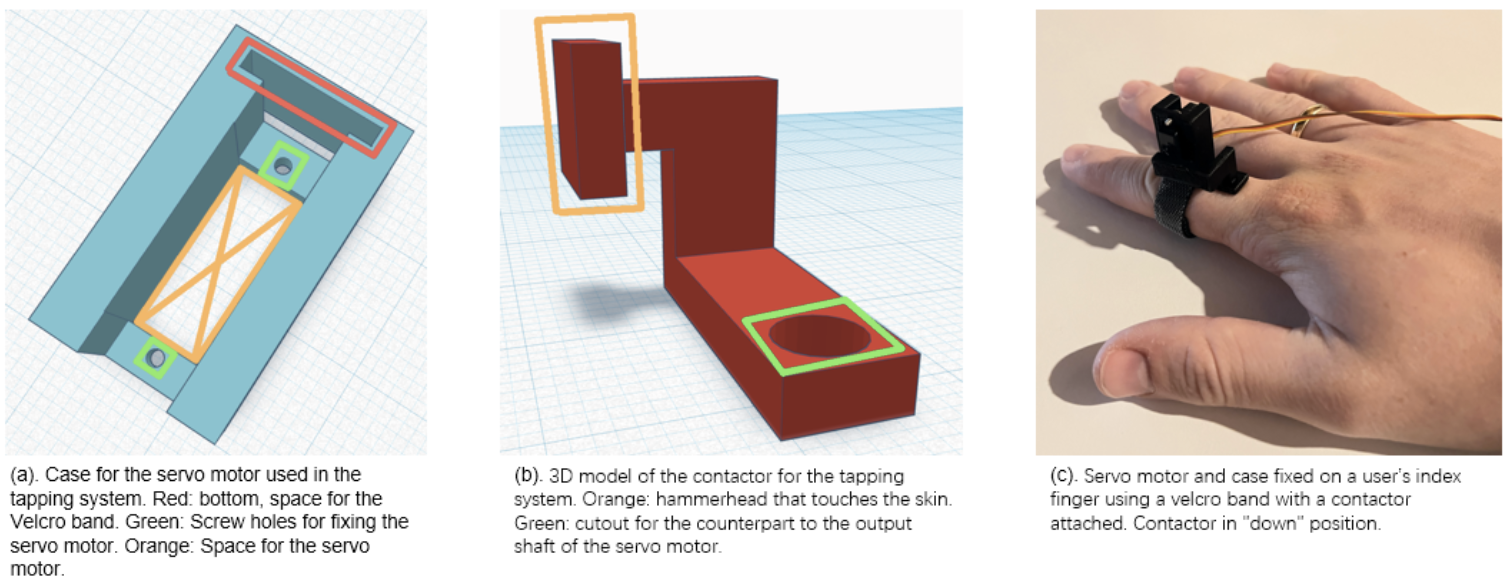
\includegraphics[width=0.5\linewidth]{src/pictures/Screenshot 2024-09-12 at 15.11.38.png}
    \caption{3D models for the case and hammer-shaped contactor, and the implementation on a user’s finger of one element of the tapping system from \cite{Fang2023}}
    \label{fig:fang-tapping}
\end{figure}
\begin{figure}
    \centering
    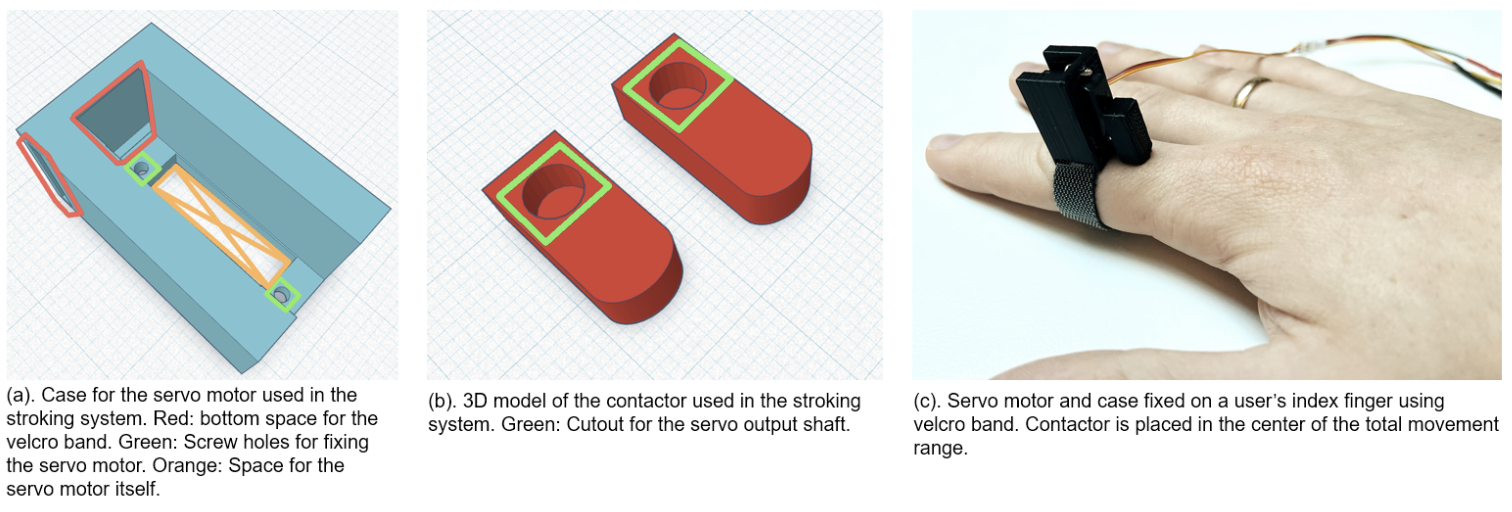
\includegraphics[width=0.5\linewidth]{src/pictures/Screenshot 2024-09-12 at 15.10.49.png}
    \caption{3D models for the case and the contactor, and the implementation on a users finger of one element of the stroking system from \cite{Fang2023}.}
    \label{fig:fang-stroking}
\end{figure}

For the tapping and stroking systems, we employed six actuators for each system, utilizing mini-servo motors (Master DS208). These motors provide an actuating force of approximately 0.1–0.2 kg and complete a 45° movement in approximately 0.1 seconds. The actuators draw around 5V and 1.75A for stroking, and 5V and 2A for tapping, based on our measurements using a 
USB Current Voltage Capacity Tester (Model: KWS-V20/V21).
Both systems are controlled via \gls{pdm} through the glove. The cases for these systems are 3D-printed using PLA. The design of the stroking system is shown in \autoref{fig:fang-stroking}, while the tapping system is depicted in \autoref{fig:fang-tapping}.

To enhance wearer comfort during prolonged use, we added a small cushion to the actuator casings for both the tapping and stroking systems. This cushion, which was not included in Fang et al.’s original design \cite{Fang2023}, and is only used for the contact area of the non-moving part of the actuator and the skin.

The tapping system delivers equal force at the same rate by applying and removing contact from the user’s skin \cite{Fang2023}. Its design follows a hammer-like structure, consisting of a servo motor housed in a PLA case and a contactor. The contactor is an 8 × 8 mm square plate that presses against the skin, connected to the servo motor’s output shaft via an L-shaped support. The design is illustrated in \autoref{fig:fang-tapping}.

The stroking system, shown in \autoref{fig:fang-stroking}, features a contactor that moves across the user’s skin while simultaneously indenting it slightly, similar to the tapping system. The contactor is a 15 × 7 × 5 mm square with a rounded bottom and is housed in a design similar to the tapping system. The servo motor is mounted on the participant’s hand, and by rotating the motor, the contactor performs a stroking motion across the skin.

All actuators are positioned near the interphalangeal joints of the fingers.











\subsubsection{Glove Design and Design Iterations}
\label{Glove_Design_Iteration}
\begin{figure}
    \centering
    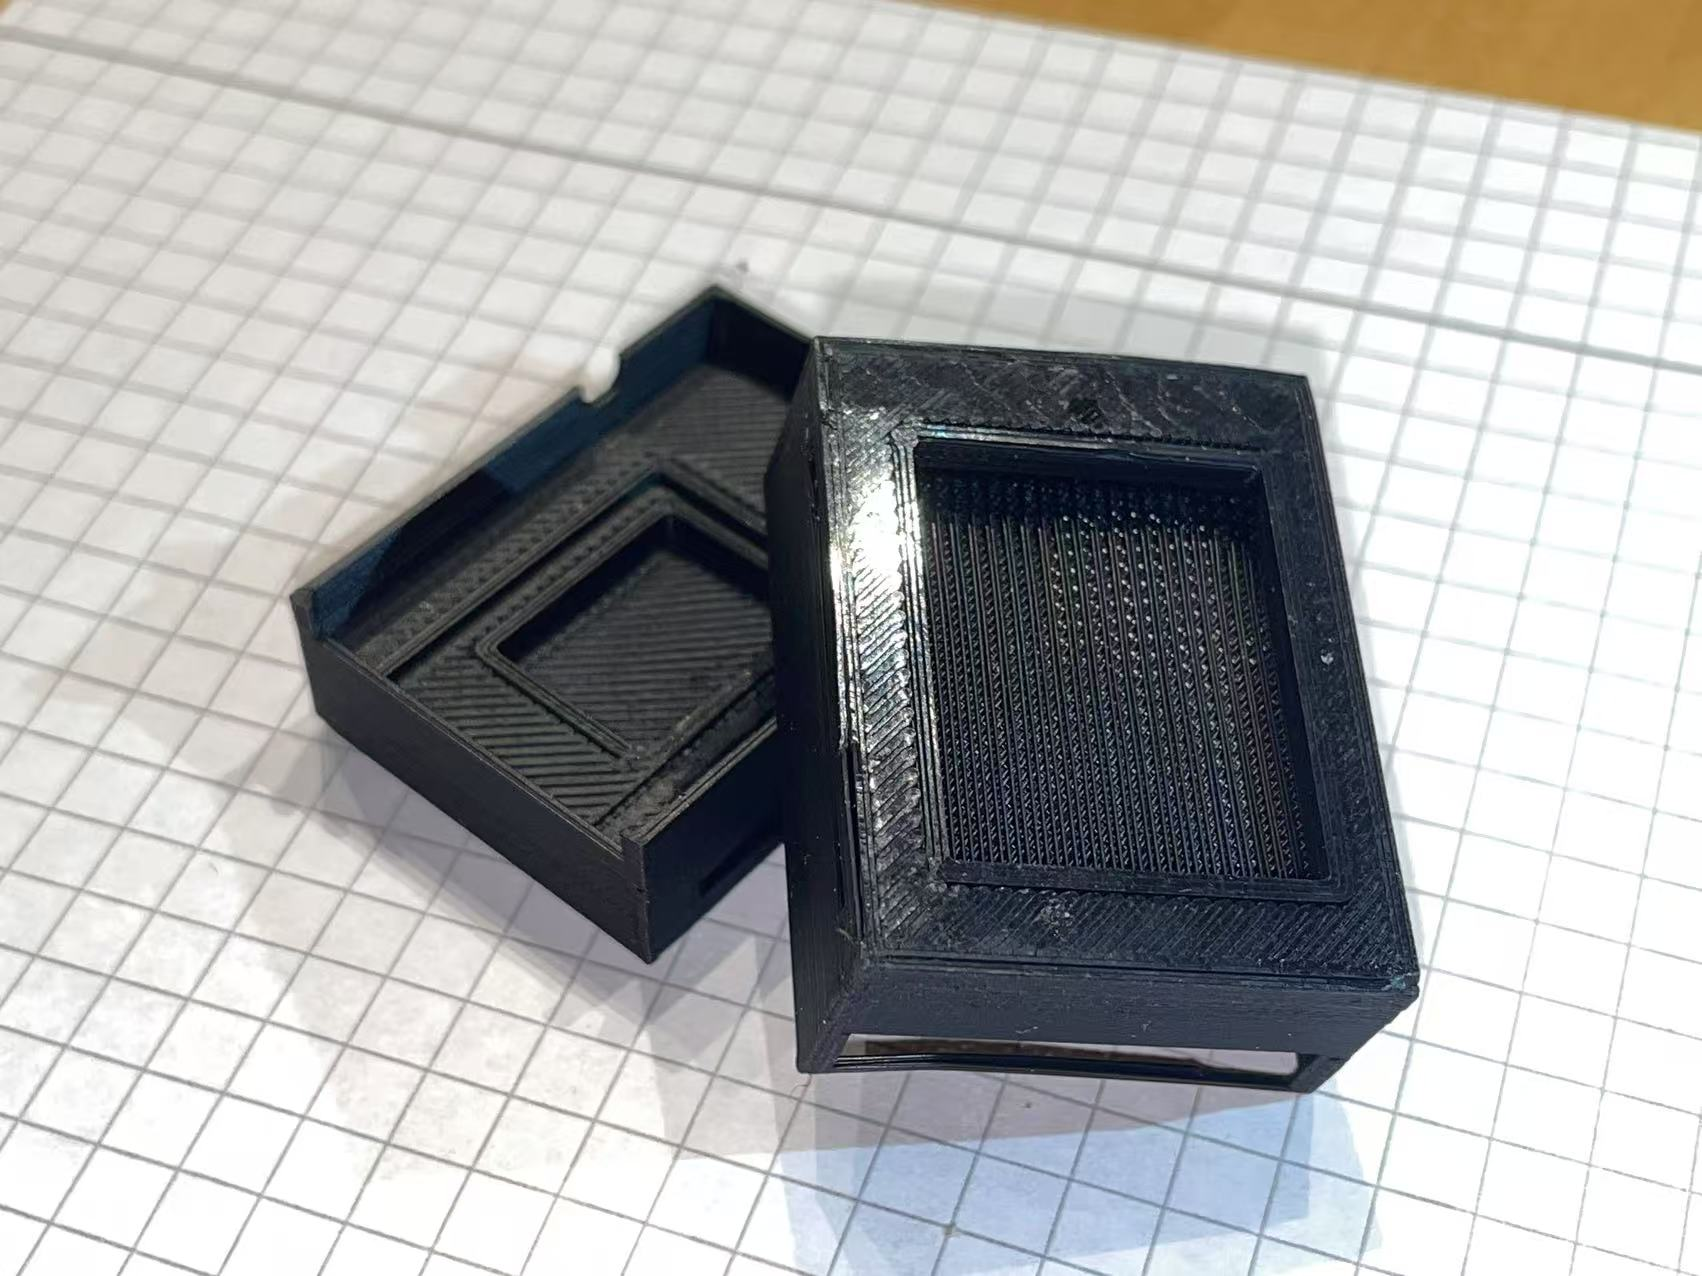
\includegraphics[width=0.5\linewidth]{src/pictures/GloveDesigns/cases.jpg}
    \caption{Final Glove- Case Design on a squared Din A5 paper for size reference.}
    \label{fig:cases}
\end{figure}

\begin{figure}
    \centering
    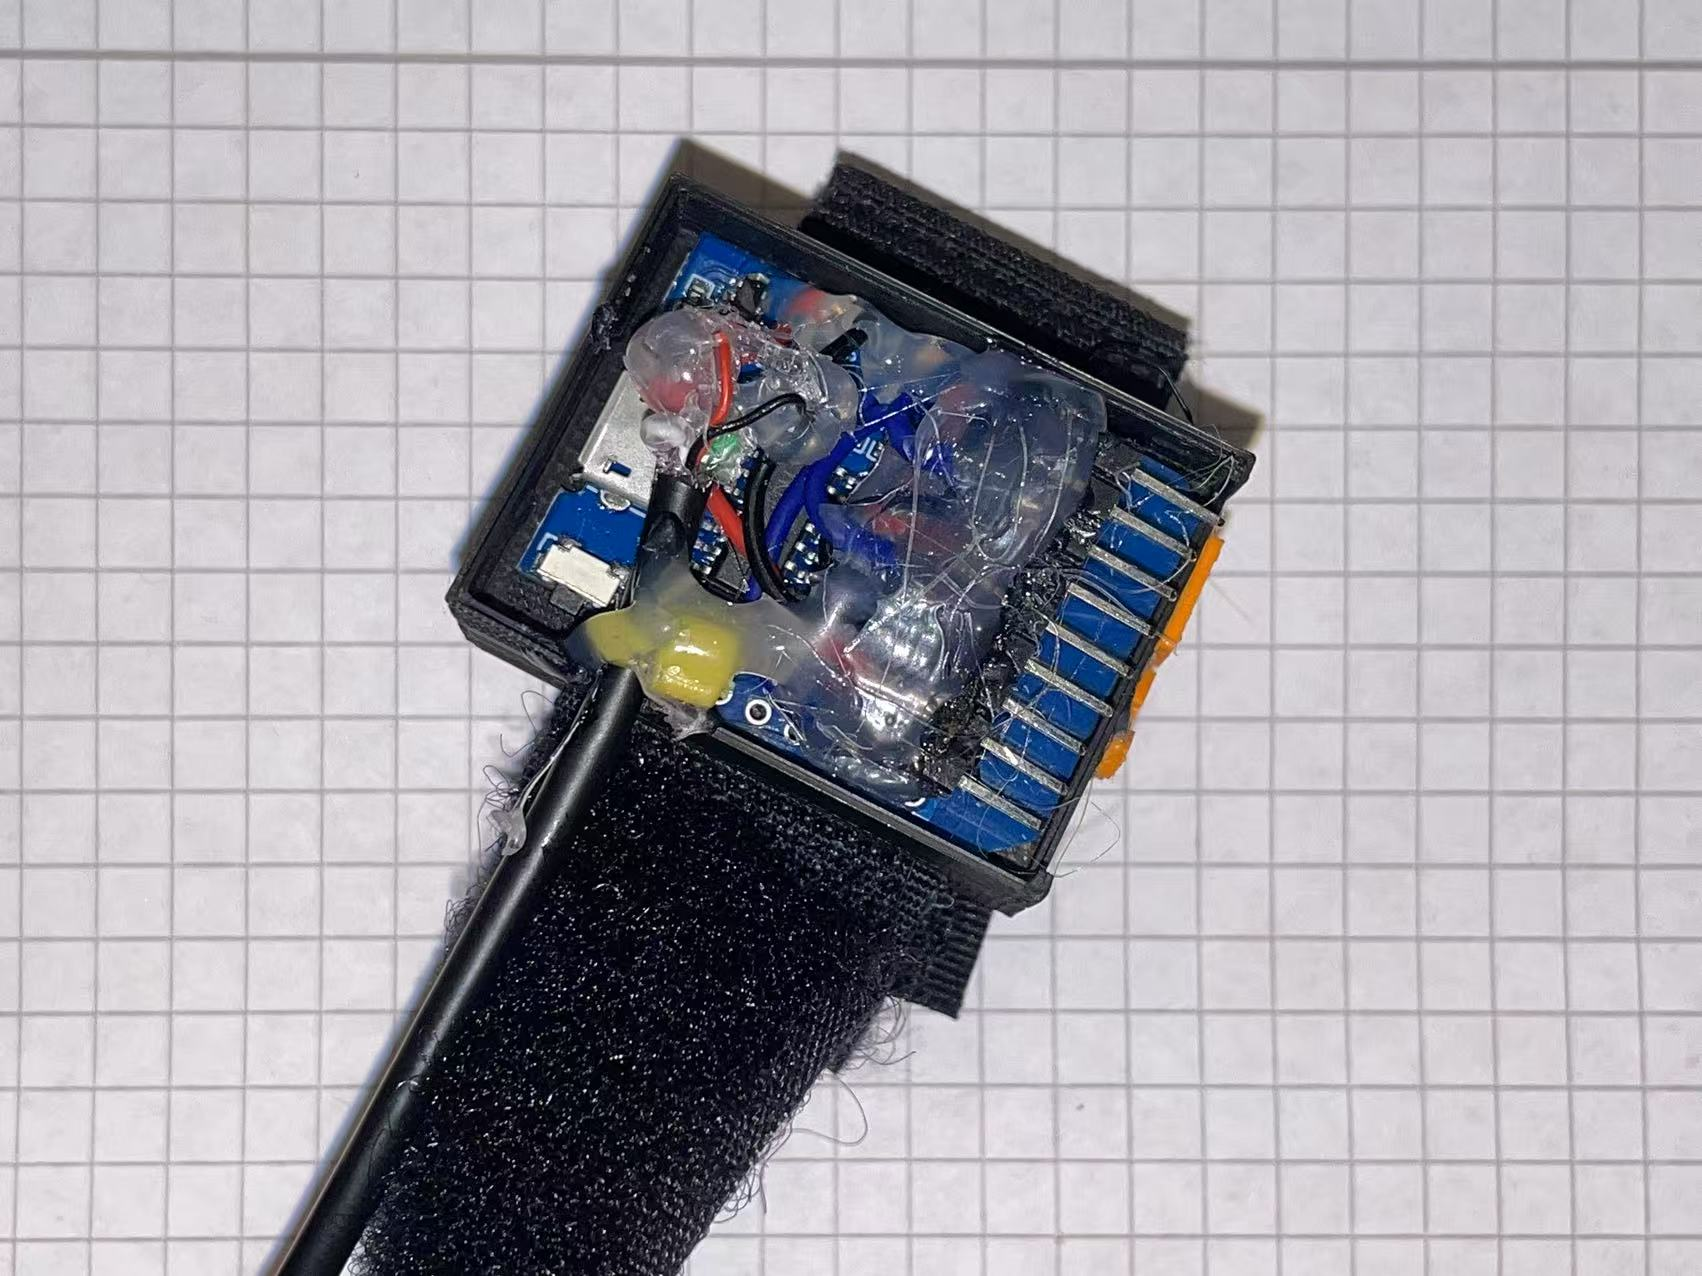
\includegraphics[width=0.5\linewidth]{src/pictures/GloveDesigns/openCase.jpg}
    \caption{Final Glove Design opened on a squared Din A5 paper for size reference.}
    \label{fig:openCases}
\end{figure}

Our final glove design, shown in \autoref{fig:final-glove-design}, incorporates the actuators described above along with a wristband. The wristband consists of a Velcro strap mounted onto a 3D-printed PLA casing with a cushion on the bottom to enhance comfort during extended wear. Herefore, we left a small hole in the bottom to fit the cusion into it due to the cushion being not soft enough due to the clue if not placed within a small indentation as showed in \autoref{fig:cases}.

The casing measures 37.6 mm × 28.75 mm × 15 mm, making it comparable in size to the Xiaomi Mi Watch Lite smartwatch (dimensions: 41 mm × 35 mm × 10.9 mm, weight: 35 g with strap, 21 g without strap)\footnote{\url{https://www.mi.com/de/mi-watch-lite/specs/}}. Also the bottom is fitted, so that the ESP8266 can fit even without glue in there and won't move.
With a open case the design is depicted here \autoref{fig:openCases}. The 9 outputs are the same as depicted in the circuit diagram in \autoref{fig:circuit-diagram}.

This design achieves our goal of creating a compact wearable device comparable to a modern smartwatch.



\begin{figure}
    \centering
    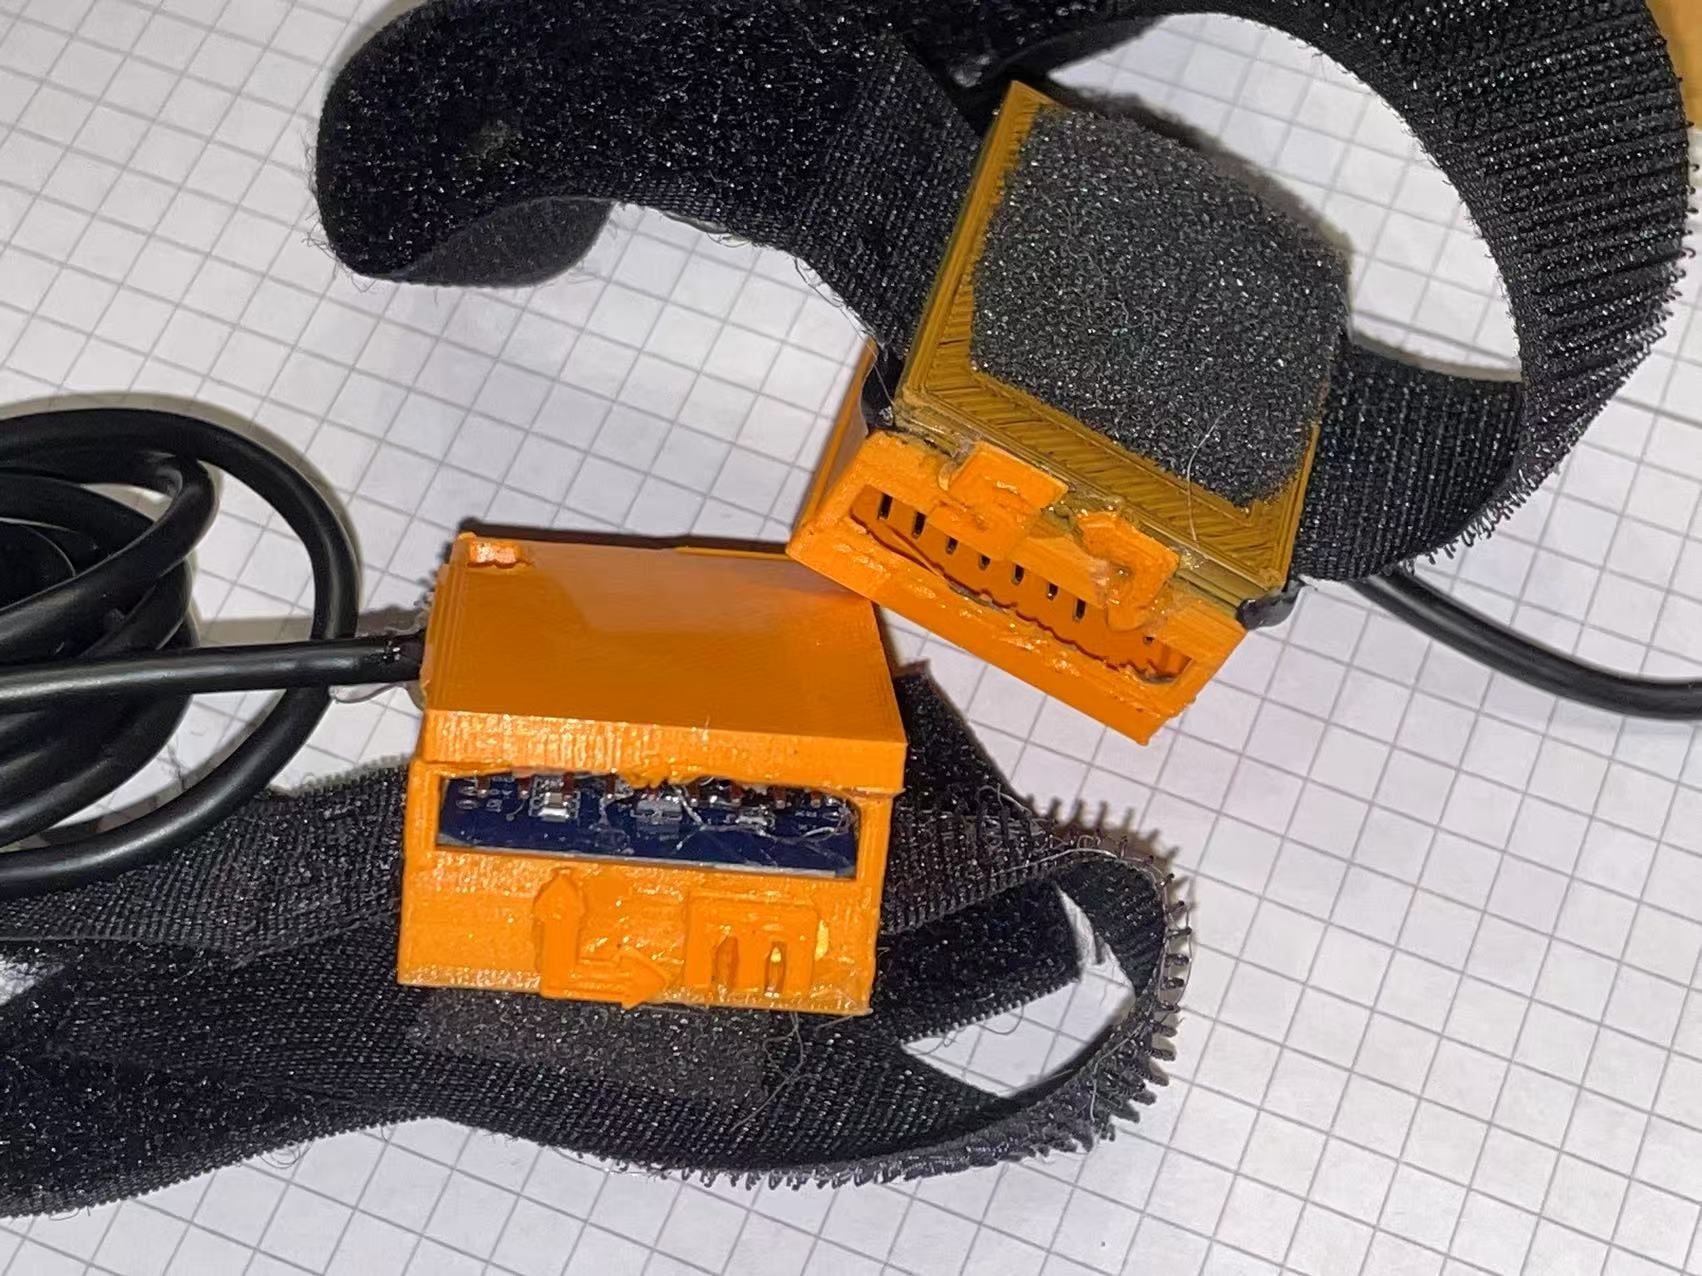
\includegraphics[width=0.5\linewidth]{src/pictures/GloveDesigns/casesFinished.jpg}
    \caption{Final Glove Design on a squared Din A5 paper for size reference.}
    \label{fig:final-glove-design}
\end{figure}


\begin{table}
    \centering
    \resizebox{\columnwidth}{!}{
    \begin{tabular}{cccccccc}
        \textbf{Protocoll}   & \textbf{Range} & \textbf{EE (R)} & \textbf{EE (T)} & \textbf{Throughput} & \textbf{Latency} & \textbf{Overhead} & \textbf{OSI-Layer}\\
        \textbf{ESP-NOW}     & 220m & 489 mW & 1042 mW           & \textbf{1 Mbps} & \textbf{~1ms} & \textbf{Small} & Layer 2\\
        \textbf{TCP / UDP}         & 100m & 214 mW & 538 mW & \textbf{54 Mbps} & ~3.3ms & Medium & Layer 4\\
        \textbf{Bluetooth}   & 60m & 141 mW & 441 mW       & ~784 Kbps & ~6ms & High & Layer 2\\
    \end{tabular}}
    \caption{Comparison of Wi-Fi, Bluetooth and Esp-Now \cite{eridani2021comparative}.\\EE stands for Energy Efficiency, R stands for receiver and T for transmitter.}
    \label{tab:comparissonESPNOW}
\end{table}

For the microcontroller, we chose to use devices from the ESP family due to their compatibility with the ESP-Now protocol. This decision was based on the protocol's advantages in terms of latency, overhead, and throughput, as highlighted in the comparison by Eridani et al. \cite{eridani2021comparative}, with their results shown in \autoref{tab:comparissonESPNOW}. As we identified those as the most important criteria for solving our  soft-real time\footnote{Soft-Real Time as defined in computational theory such as by Shin et al. \cite{shin1994real}} requirements, as we need to get the ms timings right and in order.

\begin{figure}
    \centering
    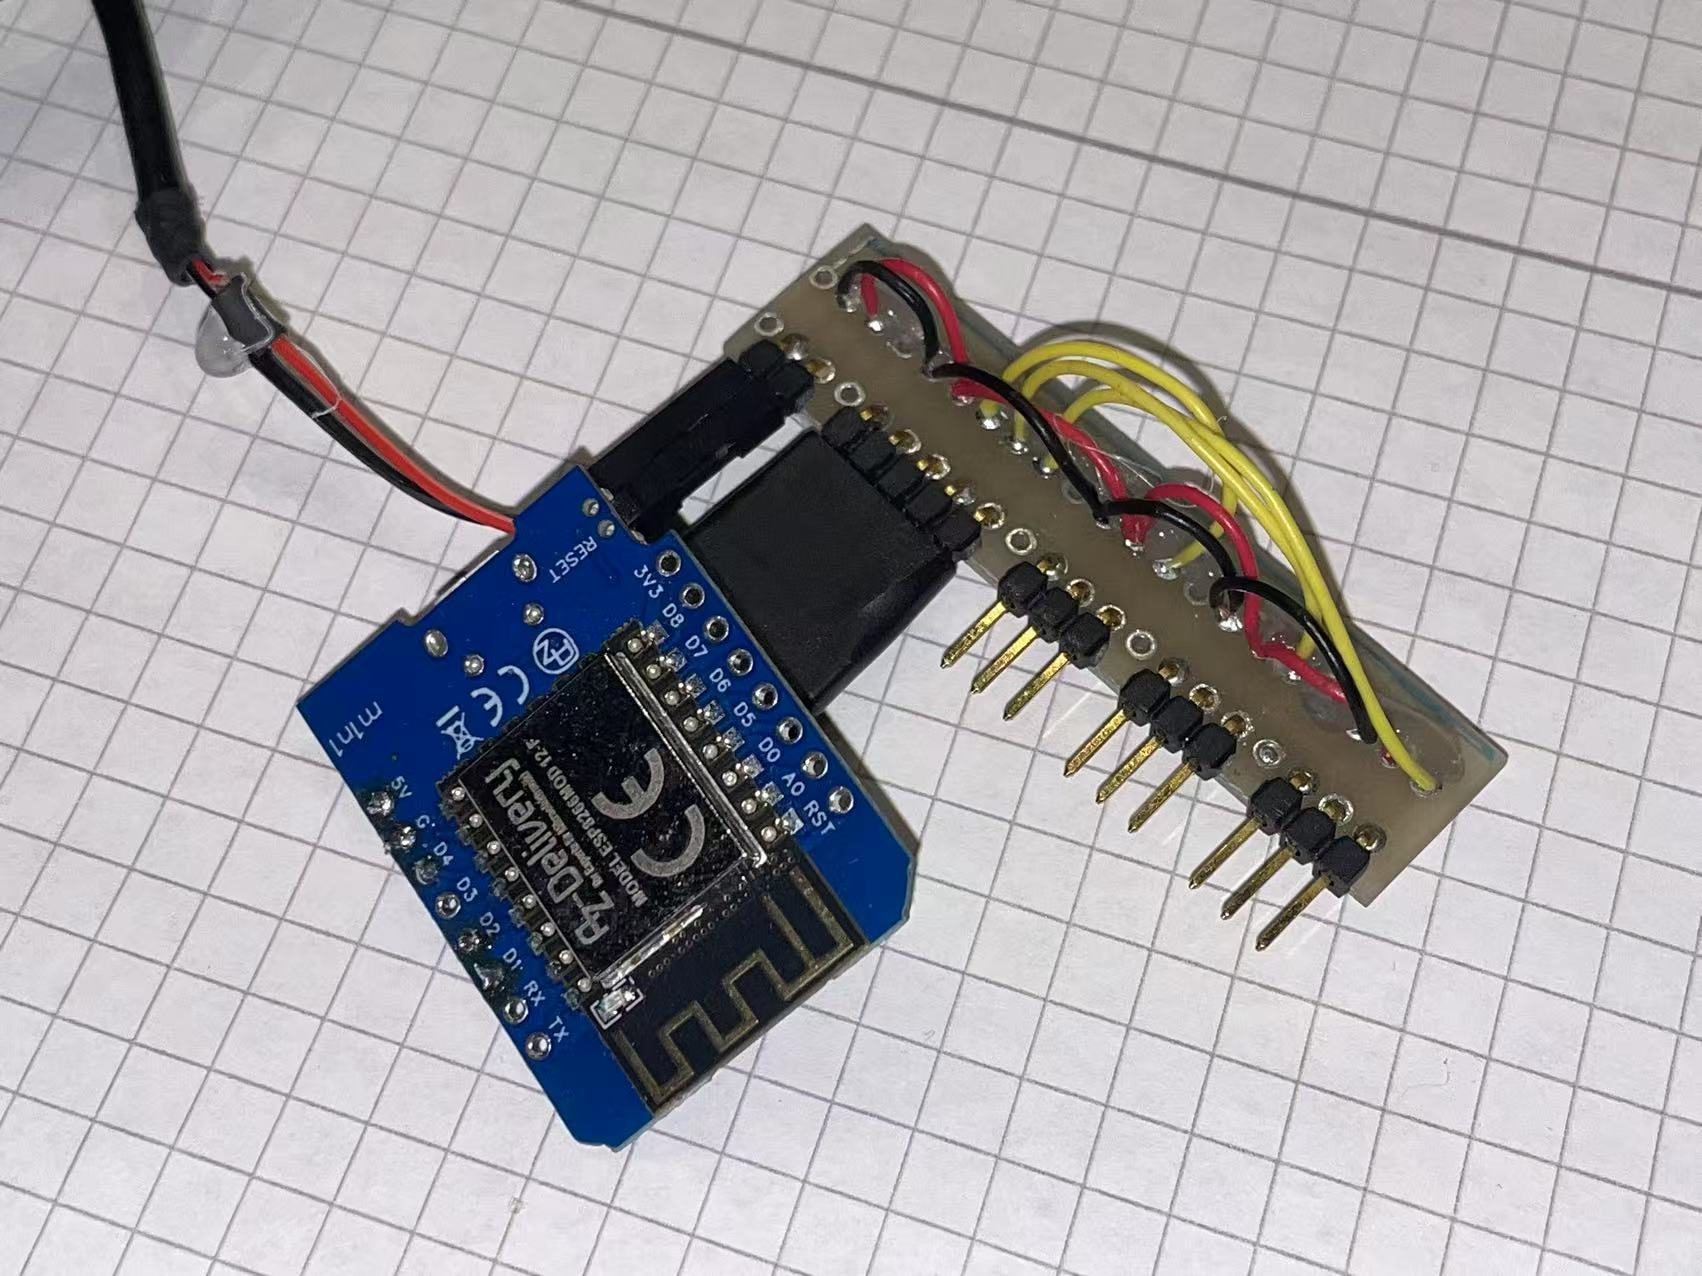
\includegraphics[width=0.5\linewidth]{src/pictures/GloveDesigns/oldDesign.jpg}
    \caption{Old design of the circuit.}
    \label{fig:oldDesign}
\end{figure}

In our initial design iteration, we used the ESP8266 microcontroller, but it was later replaced with the ESP8266 D1 Mini due to several advantages. These include its low cost (approximately €1), lightweight design (3 g)\footnote{\url{https://www.smart-prototyping.com/Mini-D1-PRO-Development-Board-ESP8266-4M-16M}}, and compact size. Both microcontrollers offer built-in Wi-Fi capabilities that provide sufficient connectivity for the entire software system. The affordability and accessibility of the ESP8266 D1 Mini make it particularly suitable for use in low-income households, enhancing the device's feasibility and reach.

The first alpha prototype version with the esp8266 D1 mini is shown in \autoref{fig:oldDesign}. As it is the \gls{mvp}, it is rather bulky with the cables attached to it. Nevertheless, the same circuit diagram as in \autoref{fig:circuit-diagram} applies for it, and it is fully operational.

\begin{figure}
    \centering
    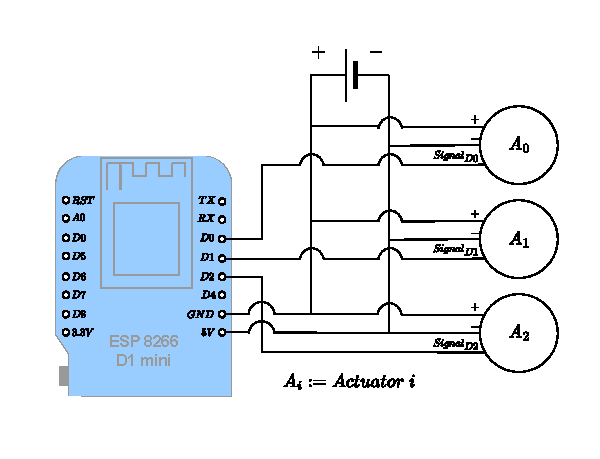
\includegraphics[width=0.5\linewidth]{src/pictures/CircuitDiagramGlove.drawio.pdf}
    \caption{Glove Circuit Diagram.}
    \label{fig:circuit-diagram}
\end{figure}


Due to the high current demands of the tapping and stroking systems, the on-board power supply of the ESP8266 was insufficient. To resolve this, we soldered an additional USB cable to the board to provide an external power supply, as shown in \autoref{fig:circuit-diagram}, that can also be seen on \autoref{fig:oldDesign} for the \gls{mvp} and in \autoref{fig:openCases} for the current one.
In the first experiment, the actuators were interchangeable and could be of the vibration, tapping, or stroking type.
We utilized the pins D0, D1, and D2 because of their \gls{pdm} capabilities.

The USB cable was connected to a standard phone charger. For testing, we used the original 10W Xiaomi USB-A charger (model: MDY-09-EW), which has a maximum output voltage of 5V and 2.0A. This served as the general power source for the system, with one charger used per glove. The design also works with a powerbank, however due to our extended experiment times we didn't use a powerbank in our study.

Furthermore, we added additional wiring to simplify mounting the actuators onto the wristband glove, ensuring better usability and stability during operation.
Which can be seen in the open version of the glove design depicted in \autoref{fig:openCases}, so that we can fit the actuators directly on it.




\subsection{Software}

This software section is divided into two parts, the webistes created for the experiment (one on the glove and one on an external laptop for testing) as well as the communication protocoll used between the gloves.



\subsubsection{Website}
\label{sub:website}
Two websites were developed for the study, adhering to the Material Design guidelines for button design and usability\footnote{\url{https://m3.material.io/}}. One website was displayed on a mobile phone (Xiaomi A2 Lite), which was hosted by the glove to control the experiment and play audio data, while the other was used to assess the participants' knowledge.

The website for controlling speech output and vibrations is shown in \autoref{fig:Website-Design}. It was designed using a responsive framework, enabling compatibility with other devices capable of running modern browsers. During the study, we used the Google Chrome browser on the smartphone.

The website could be accessed within the "Master Glove" Wi-Fi network (SSID: Master Glove) using the URL \url{192.168.4.1}.
The preset buttons on the website correspond to those used in the studies.
Upon pressing a button, the master controller receives the associated word or letter, as well as whether \gls{ost}-Encoding is activated (inactive for sequential input).
The master controller then sends this data to the slave controller.

The website plays the corresponding audio for the selected character using a JavaScript text-to-speech converter, as the master controller was not connected to the internet.
After the specified offset detailed in the audio-vibration offset section, the vibration begins, aligned with the encoding chords and tailored to finger sensitivity.
Both, the audio and vibrations automatically stop after five minutes, providing a break for the conductor to test the participant, as outlined in the study protocol.

\begin{figure}
    \centering
    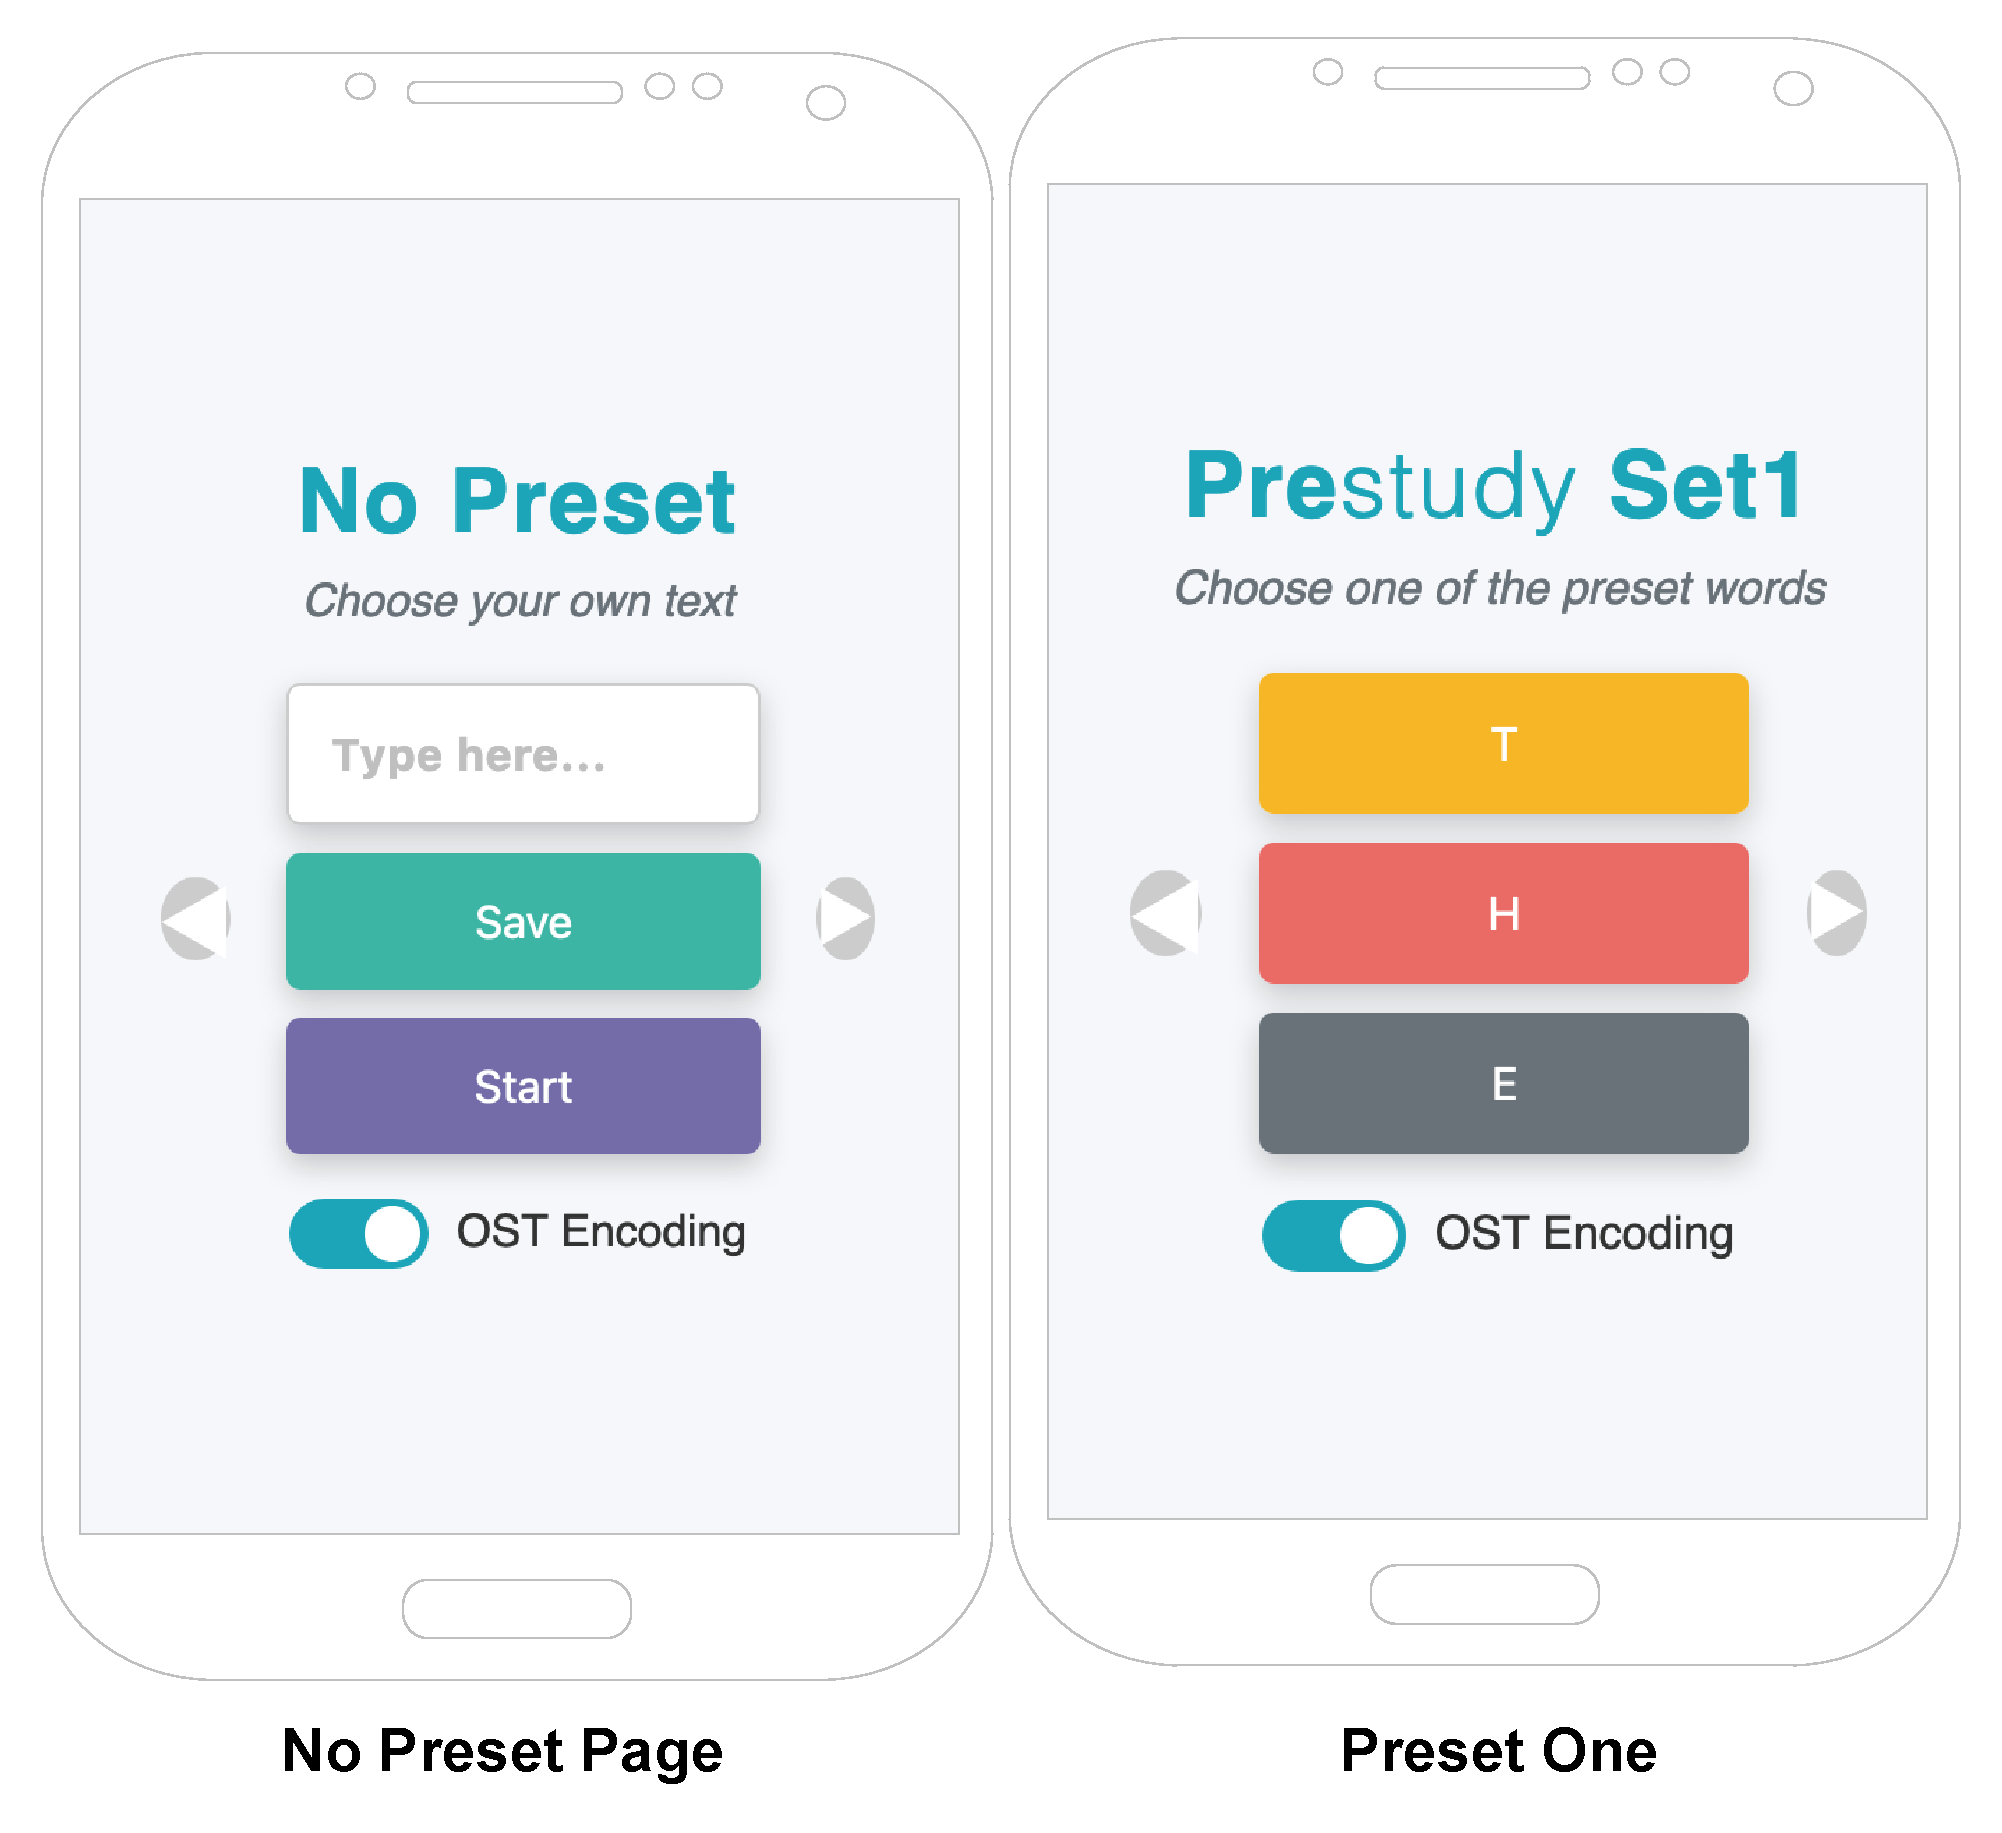
\includegraphics[width=0.5\linewidth]{src/pictures/MobileWebsiteVersion.drawio.pdf}
    \caption{Website Design in a Mobile Phone.}
    \label{fig:Website-Design}
\end{figure}

The second website, shown in \autoref{fig:testing-site-Design}, was designed solely for testing participants' knowledge. It ran on a Firefox browser on a Fujitsu laptop (model: VFY A5440M15B70E) with Ubuntu.

Additionally, instead of displaying the pressed character, we only showed asterisks ("*") to avoid distracting the user. This approach followed the idea of the "stars-only feedback" condition from Seim et al. \cite{Seim2014}, allowing participants to focus on the order rather than the specific characters.

The same laptop was also used to run Gwelled, the game employed in Fang et al.'s study \cite{Fang2023}, during the learning session.

\begin{figure}
    \centering
    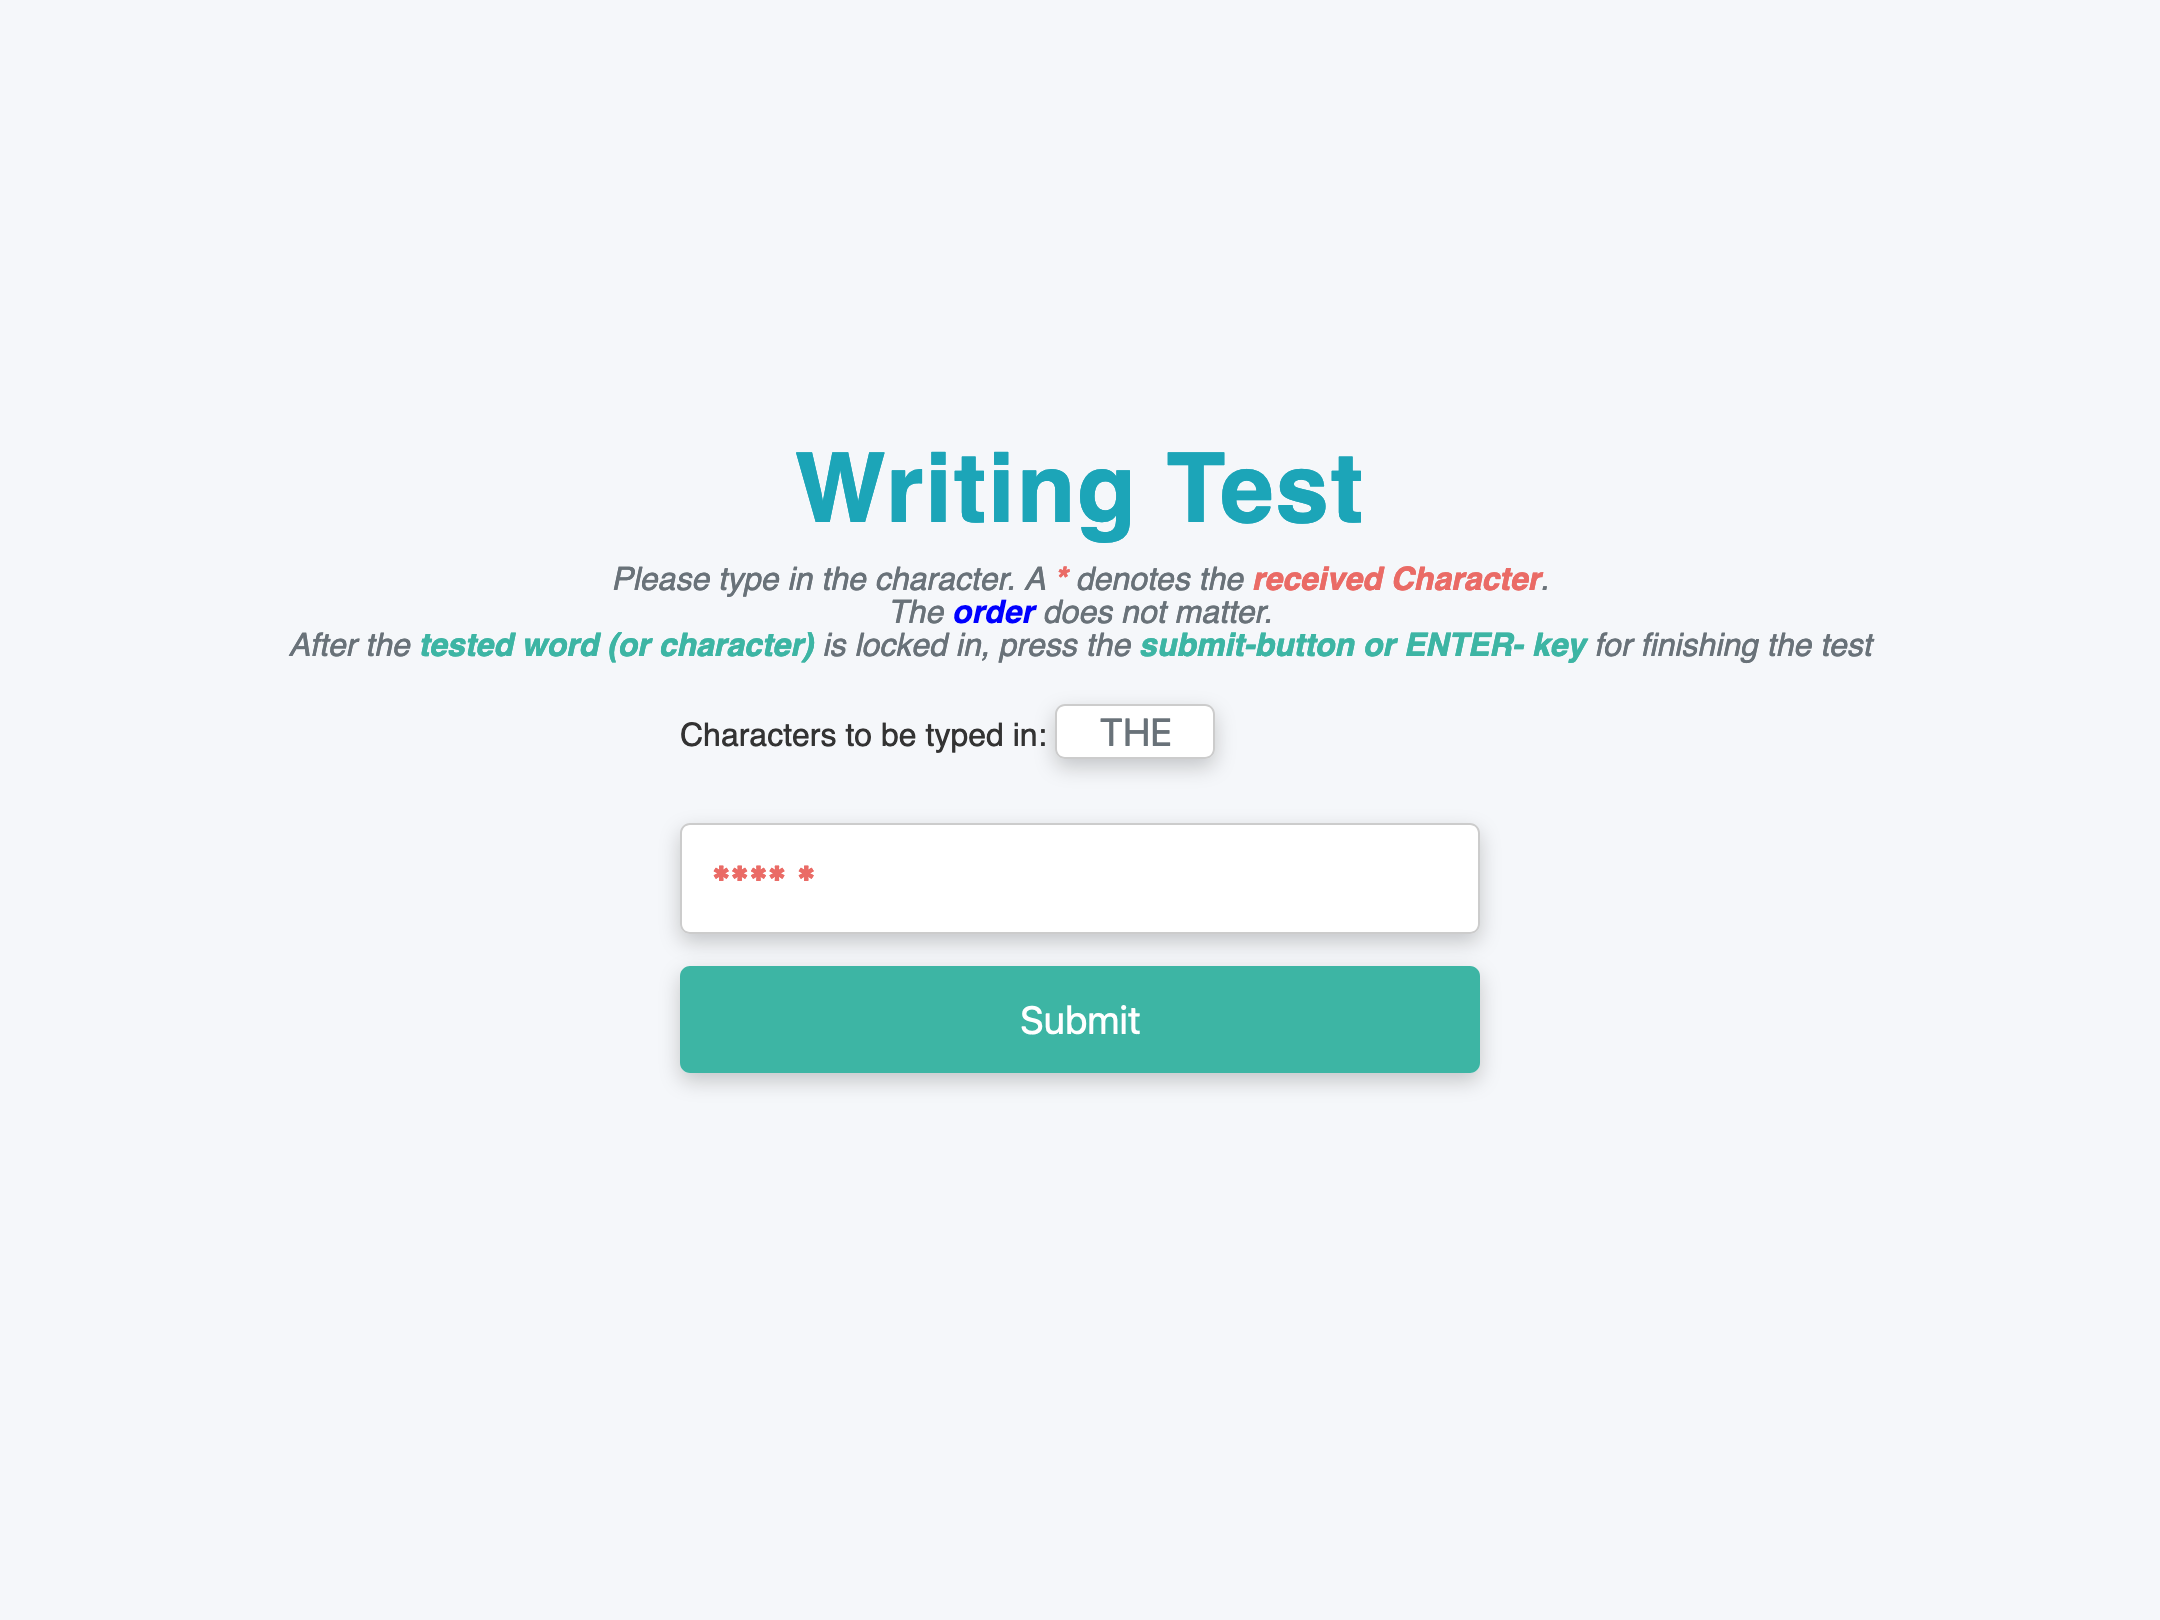
\includegraphics[width=0.5\linewidth]{src/pictures/testingSite.png}
    \caption{Testing Site for the Writing Test.}
    \label{fig:testing-site-Design}
\end{figure}


\subsubsection{Communication between the gloves}
Both gloves operate using a master-slave configuration, with the left glove functioning as the master and the right glove as the slave. To ensure flexibility in actuator motor types and encoding schemes, we implemented a layered architecture within both the master and slave gloves.

For communication, the slave glove employs a listener that, upon receiving a message, triggers a callback function to determine how the data should be processed.

The slave glove can receive two types of data. The first type is the activation sequence, which consists of a series of activation requests and pauses in between. Once this sequence is received, the slave waits for the second type of data—a timing index indicating when the next character should be played.

This approach ensures precise synchronization, as the timing index is transmitted during the pauses between characters, preventing significant timing discrepancies. To meet the requirements of low overhead, fast latency, and high throughput, as outlined in section \ref{Glove_Design_Iteration} 
and illustrated in \autoref{tab:comparissonESPNOW}, we leverage this speed to maintain accurate timing without the need to wait for a connection to be fully established.



\subsection{Encoding Scheme}
This section provides an overview of the encoding methods used in our study. First, we introduce the encoding of chords, which we employ in both of our studies. Here, we differentiate between the sequential approach that we use and the \gls{ost} encoding approach.

The section also discusses the finger activation sequence to ensure alignment with previous works. The second subsection addresses the offset between the audio and the activation sequence that we employ, explaining which method we use and the rationale behind our choice.

The third part focuses on the selection of isograms for the words used during training. We explain why we believe these words to be the most appropriate and demonstrate, using information theory, that they have similar entropy. This selection ensures that the words used for learning are of comparable complexity. Additionally, we explain why our chosen words form a partial pangram.


% We employed two encoding schemes: the \gls{ost} encoding scheme and the spatial-temporal encoding scheme.
% For both schemes, we followed the same finger activation order as Luzhnica et al. \cite{Luzhnica2017}, which demonstrated that activating the fingers in a specific sequence was beneficial.

% The precise timing of these activations is critical to ensure comparability with previous studies.
% The specifications for these timings are detailed in this subsection.

% Additionally, this section explains how we spaced the audio and tactile sensations by comparing our task to similar studies in the field.

% Finally, we discuss the selection of isograms that, together, form part of a pangram.
% We compare these words with those used in previous studies and highlight their shortcomings for our task.
% Specifically, we demonstrate the difference in entropy between the Braille encodings of these words, which provides insight into their effectiveness for our encoding task.


\subsubsection{Encoding Chords}
Encoding Braille words as tactile chords is not straightforward because several considerations must be taken into account, such as how to encode a chord in a way that prevents all fingers from vibrating simultaneously, as this was shown to be ineffective by Seim et al. \cite{Seim2014}, who demonstrated that participants often struggle to distinguish stimuli. Additionally, when offsetting each of the tactile sensations, further considerations must be made, such as: "How long are the sequences activated?" "In which order are the tactile sensations delivered to the fingers?" "How long and where are breaks placed during activation?" and "What activation protocol should we use?" To address these questions, we orient ourselves based on previous works.

For the activation protocol, we use two different encodings, which we compare against each other in the second study. We employ the \gls{ost} encoding developed by Luzhnica et al. \cite{Luzhnica2018, Luzhnica2018a, Luzhnica2017, Luzhnica2016}, as shown in \autoref{fig:chord_encoding}, to encode the chords. The \gls{ost} encoding uses a gap $p$ of 10 ms, following the value named ($g$) used in \cite{Luzhnica2018}, with the same finger stimuli order and tactile thresholds that align with the findings of \cite{Duncan2007}. Additionally, we incorporate the sequential encoding approach used by Seim et al.

The \gls{ost} encoding has several advantages, such as enhanced throughput, as previously outlined. Furthermore, compared to simultaneous encoding, which often leads to difficulties in distinguishing stimuli \cite{Seim2014}, the \gls{ost} encoding has proven more beneficial for learning \cite{Luzhnica2018}. In the first study, we use only the \gls{ost} encoding.

Luzhnica et al. \cite{Luzhnica2017} found that the order in which tactors are activated during overlapping spatiotemporal stimulation impacts the ability to accurately identify stimuli. Prioritizing the activation of tactors, starting with the most sensitive areas, significantly improves accuracy. Building on these findings, we prioritize the fingers according to their known sensitivity order (from index to ring finger), as described by \cite{Luzhnica2017}, \cite{Hoggan2007}, \cite{VegaBermudez2001}, and \cite{Duncan2007}. This prioritization follows the approach outlined by \cite{Luzhnica2017} to enhance perception accuracy.

Studies on temporal acuity indicate that individuals can discriminate between successive taps on the skin with a gap as small as 5 ms \cite{Luzhnica2017, Katz2013}. Luzhnica et al. found that gaps of 10 ms and 20 ms between taps did not significantly impact perception accuracy. Based on this, we chose a gap of 10 ms, as shown in \autoref{fig:audio_vibration_gap}, which is greater than the minimum discriminative gap of 5 ms established by \cite{Luzhnica2017}. This 10 ms gap has been used for \gls{ost} encodings in previous studies \cite{Luzhnica2018, Luzhnica2016}.

During both studies, we use the same intensity for vibration, as \cite{Luzhnica2017} found that varying vibration intensities between tactors does not lead to higher accuracy, even when prioritization by sensitivity is applied. Therefore, we maintain consistent intensities across all tactile sensations.

For the base duration $d$, we use 200 ms, with a between-letter gap (bl) based on the average durations of dots (100 ms) and dashes (300 ms) from \cite{Seim2018} and dots (200 ms) from \cite{Pescara2019}. The 200 ms duration aligns with the recommendations of \cite{Luzhnica2018}, who suggest this interval to separate subsequent letters. While this duration is shorter than those used in some language-teaching studies, such as \cite{Seim2014a}, it fits well within the 100–300 ms range used for keypad learning chords by Seim et al. \cite{Seim2017}.


\begin{figure}
    \centering
    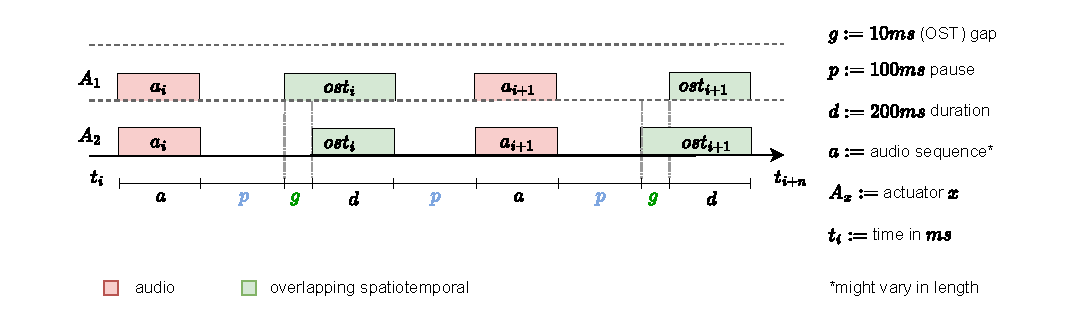
\includegraphics[width=\linewidth]{src/pictures/audio_vibration_diagram.drawio.pdf}
    \caption{Audio vibration offset.}
    \label{fig:audio_vibration_gap}
\end{figure}

\subsubsection{Audio-Chord Offset}
For the offset between audio and vibration, we adopt the same value as used in \cite{Seim2017} for Braille learning, which is 100 ms, as shown in \autoref{fig:audio_vibration_gap}.

For stroking and tapping, we follow the setup described by \cite{Fang2023}, where each finger is stroked or tapped once. However, we use the \gls{ost} encoding with the same \gls{ost} gap and pause time, as illustrated in \autoref{fig:audio_vibration_gap}, so the only difference between the affective and discriminative touch setups lies in the base duration $d$. Since this is the first study, to our knowledge, investigating \gls{ost} with stroking or tapping for affective touch, we use this pattern without any additional prior timing guidelines, except for the passive learning encoding found in Fang et al. \cite{Fang2023}.


\subsubsection{Isogram Selection and carry-over effect minimisation}
\begin{figure}
    \centering
    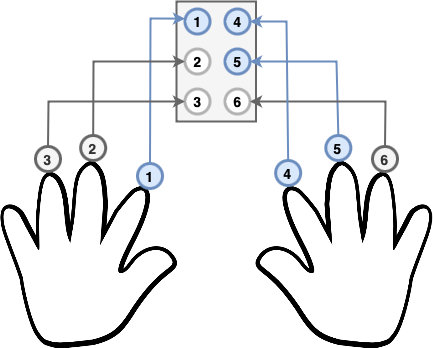
\includegraphics[width=0.5\linewidth]{src/pictures/handBrailleEncoding.drawio.png}
    \caption{Encoding of the character D as an example for hand encodings.}
    \label{fig:hand-encoding}
\end{figure}


When participants are passively learning to type using different actuators, we use a segment of a pangram \cite{Brooke1987}, following the methodology of Seim et al. \cite{Seim2018, Seim2016}. This approach is intended to mitigate the \enquote{carryover effect} \cite{MacFie1989, Brooks2012}, which occurs when participants are influenced by previously learned data, either through stress or prior knowledge.

To ensure a fair comparison and avoid the carryover effect, we taught participants different characters with equal complexity for each actuator. Pescara et al. \cite{Pescara2019} defined complexity by creating patterns of equivalent length and difficulty, based on the number of dash and dot transitions in Morse code. Inspired by this approach, we use entropy, as defined in information theory \cite{Gray2011, Shannon1948, Shannon2001}, to quantify the underlying complexity.

To achieve this, we encoded each Braille dot with a number from 1 to 6, following the methodology of \cite{Yang2017}. The dots correspond to positions on the left hand (index to middle finger) and right hand (index to middle finger), as illustrated in \autoref{fig:hand-encoding} for the Braille character \enquote{D}. Each character is thus represented as a set of numbers corresponding to the Braille dots.

Using this encoding, we calculated the probability \( P(d) \), where \( d \) represents a ``dot at position \( i \).'' We used the standardized English Braille alphabet, consisting of 26 characters. The probability distribution for each dot being present in a character is calculated as:

\[
P(d = X) = \frac{\|\{d \in c \mid c \in A\}\|}{\|A\|}
\]

where \( A \) represents the 26-letter English alphabet. The results are summarized in \autoref{tab:dot-probability}, showing the occurrence of each Braille dot and its corresponding probability across the alphabet.

\begin{table}[!ht]
\centering
\resizebox{.70\columnwidth}{!}{
    \begin{tabular}{c|c|c|c|c|c|c}
        Dot $d$            & \textcircled{1}& \textcircled{2}& \textcircled{3}& \textcircled{4}& \textcircled{5}& \textcircled{6}\\
        Occurrences     & $20$ & $14$ & $15$ & $15$ & $13$ & $6$\\
        $P(d)$     & $0.7692$ & $0.5384$ & $0.5769$ & $0.5769$ & $0.5$ & $0.2307$\\
    \end{tabular}}
    \caption{Probability for each dot occurring.}
    \label{tab:dot-probability}
\end{table}

Using these probabilities for each dot \( P(d) \), we then computed the entropy \( H(c) \) for each character \( c \) using the entropy formula:

\[
H(c) = \sum_{d \in C} P(d) \times \log_2 P(d)
\]

This measures the amount of information in bits per character. The calculated entropies for each character \( c \) are presented in \autoref{tab:entropy-letter}.

\begin{table}
    \centering
    \resizebox{\columnwidth}{!}{
    \begin{tabular}{lccccccccc}
        Character $c$   & \braille{a} A& \braille{b} B& \braille{c} C& \braille{d} D& \braille{e} E& \braille{f} F& \braille{g} G& \braille{h} H& \braille{i} I\\
        $H(c)$ in bits         & $0.2912$ & $0.6458$ & $0.749$ & $1.249$ & $0.7912$ & $1.1036$ & $1.6036$ & $1.1458$ & $0.8124$\\\hline
        Character $c$   & \braille{j} J& \braille{k} K& \braille{l} L& \braille{m} M& \braille{n} N& \braille{o} O& \braille{p} P& \braille{q} Q& \braille{r} R\\
        $H(c)$ in bits         & $1.3124$ & $0.749$ & $1.1036$ & $1.2068$ & $1.7068$ & $1.249$ & $1.5614$ & $2.0614$ & $1.6036$\\\hline
        Character $c$   & \braille{s} S& \braille{t} T& \braille{u} U& \braille{v} V& \braille{w} W& \braille{x} X& \braille{y} Y& \braille{z} Z& ~\\
        $H(c)$ in bits         & $1.2703$ & $1.7703$ & $1.2372$ & $1.5918$ & $1.8006$ & $1.695$ & $2.195$ & $1.7372$ & ~\\
    \end{tabular}}
    \caption{Entropy for each Braille letter rounded to $4$ decimal places.}
    \label{tab:entropy-letter}
\end{table}

We evaluated words used in previous studies, such as ``add,'' ``a,'' and ``bag'' from Seim et al. \cite{Seim2014a, Seim2014}, with entropy values of \( 2.7891 \), \( 0.2912 \), and \( 2.793 \) bits, respectively, and the words ``The,'' ``Lazy,'' and ``Dog''  from Seim et al. \cite{Seim2018}, with entropy values of \( 3.9597 \), \( 5.4531 \), and \( 4.2278 \) bits, respectively.

Next, we searched for a partial pangram composed of three words for the three actuators by going through the English dictionary with word-length of  3\footnote{\url{https://www.dictionary.com/e/word-finder/3-letter-words/}}, while ensuring that the words did not share the same characters and had similar complexity and character length, and are commonly used\footnote{As we didn't interview native speakers we needed to ensure they knew the words}. 
We selected the words ``the,'' ``old,'' and ``pub,'' as shown in \autoref{fig:braille_prestudy_characters}, with entropy values of \( 3.9597 \), \( 3.728 \), and \( 3.6969 \) bits, respectively. These words were deemed more suitable for our task due to their similar entropy values and simplicity, as many of our participants are non-native English speakers. These words were used in the first and second studies (for the second study, we used ``old'' and ``pub'' due to their closer similarity in entropy).

\begin{figure}
    \centering
    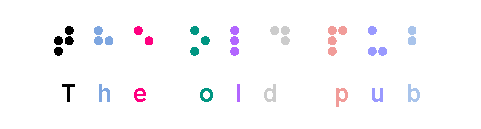
\includegraphics[width=.75\linewidth]{src/pictures/braille_prestudy_characters.drawio.pdf}
    \caption{Sentence used in the pre-study and its braille part.}
    \label{fig:braille_prestudy_characters}
\end{figure}
 











 \section{Study design}

\begin{figure}
    \centering
    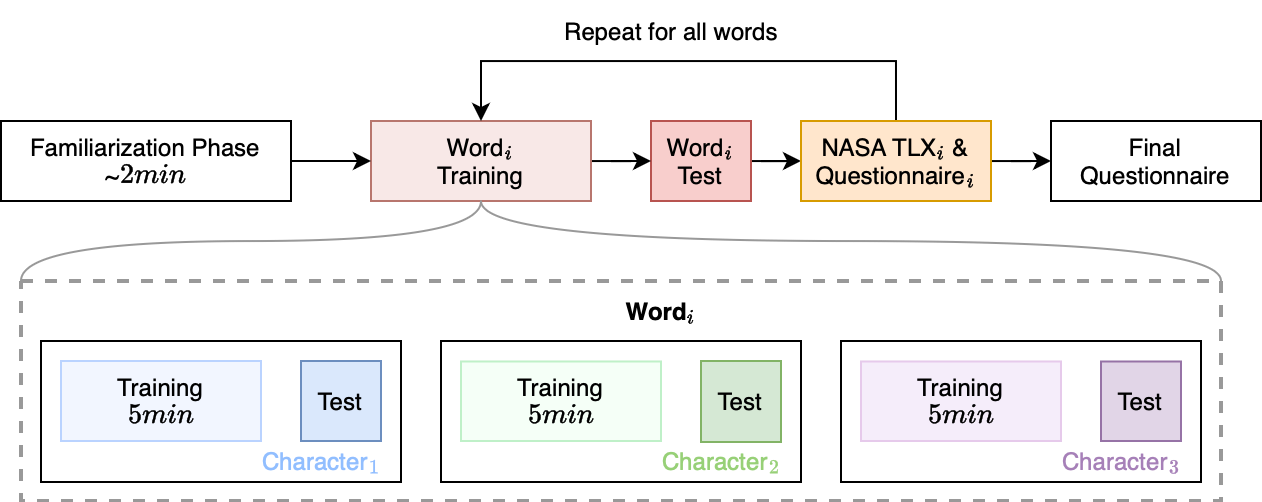
\includegraphics[width=0.75\linewidth]{src/pictures/StudyData/Study_design.drawio.png}
    \caption{Study design.}
    \label{fig:study-design}
\end{figure}

Our study is inspired by the work of Pescara et al. \cite{Pescara2019} and Fang et al. \cite{Fang2023}, and it is divided into two distinct phases. The first phase addresses our first research question: "RQ1: Is there a difference between affective and discriminative touch for both hands using the OST?" This phase is followed by a pre-study. The second phase aims to answer our second research question: "RQ2: Is there a significant difference between using the OST and the SEQ encoding?" In both studies, we focus on teaching uncontracted, alphabetic English Braille, known as Grade One Braille \cite{Troughton1992, Alnfiai2017}.

Similar to Seim et al. \cite{Seim2016, Seim2018}, our studies focus on learning words. However, we use a different set of words than those employed in their research. In the first study, we aim to assess the effectiveness of various stimuli and examine the impact of affective versus discriminative touch using the \gls{ost} encoding. This will be combined with different stimuli to teach Grade One Braille. In the second study, we investigate the differences between using the \gls{ost} and \gls{seq} encodings.

For both studies, we employed a balanced randomized Latin square design, similar to the method used by Huang et al. \cite{Huang2010}, a technique frequently applied in educational and psychological research \cite{Richardson2018}. The study procedures are illustrated in \autoref{fig:study-design}. As shown in the figure, each study begins with a familiarization phase lasting approximately 2 minutes. This phase includes using the testing website \autoref{fig:testing-site-Design} and its input method to familiarize participants with the setup, followed by a brief session of the game Gwelled to help participants acclimate to the game.

The familiarization phase is followed by word training, during which participants use the specific actuator attached to their fingers. For this, we used a Velcro band, similar to the setup used in previous studies \cite{Vaio6810, Fang2023}, enabling comparability with \cite{Fang2023}, which also investigated discriminative and affective touch. For the first study, we used the respective actuator according to the balanced Latin square design, consisting of vibration, tapping, and stroking, with the \gls{ost} encoding employed. In the second study, we used only the vibration actuator, but the encoding was changed according to the balanced Latin square design to either \gls{seq} or \gls{ost}.

During word training, each word is taught letter by letter. The training phase for each letter is followed by a test. In the letter training phase, participants play Gwelled, which was used in previous studies by Fang et al. \cite{Fang2023}, Donchev et al. \cite{Donchev2021}, and Pescara et al. \cite{Pescara2019} for 5 minutes. This serves as a distraction task while they receive their respective stimuli. Throughout this phase, we log user inputs, clicks, game scores, and the time played. This data allows us to assess participant focus in relation to the type of actuator used and evaluate the test results.

To ensure data validity, we monitored the average click count to avoid significant drops between letters with the same stimulus. For the character test, we use the testing site shown in \autoref{fig:testing-site-Design}.

After participants learn three characters, they complete a word test consisting of a word formed from the three learned characters. The word test is conducted on the same website.

During the testing phase, participants do not see their typed information to minimize distractions and encourage better performance, as detailed in \autoref{sub:website}. For each test, participants are given three attempts to reproduce the Braille character chord, following the setup used in previous works \cite{Fang2023, Seim2015, Fang2023a}. After all three characters of a word (as shown in \autoref{fig:braille_prestudy_characters}) have been learned, participants complete a NASA TLX \cite{hart1988development} questionnaire, as well as our own questionnaire assessing the perceived usefulness of the system. Once all conditions (each actuator for the first study or each encoding for the second) are completed, participants fill out a final questionnaire directly comparing the conditions to each other. This final questionnaire aims to gather objective scores for the conditions and determine participants' preferences and feedback. The questionnaires are provided in the appendix.

Since we only have two conditions for the second study, we used only the two Braille words \braille{old} (OLD) and \braille{pub} (PUB), as depicted in \autoref{fig:braille_prestudy_characters}, for learning/testing.
 %7
%  \include{tex/chapter/implementation}     %->22

 
 \chapter{Analysis}
\label{ch:Analysis}



This section analyzes the results of the collected data from the first and second studies. For both studies, we begin by analyzing the participant data, followed by an assessment of how the participants perceived the different tests in terms of difficulty, using the NASA-TLX and questions related to the comparison of the setups. Specifically, we focus on which setup participants found to be better. Next, we examine the actual performance results to compare perceived performance with actual performance.

To describe the Braille-dot components, we represent the keys using their respective numbers within a dot, as shown here: \textcircled{i} for character $i$, similar to the figures presented previously.

\subsection{First Study}

\begin{table}
\resizebox{\columnwidth}{!}{
    \centering
    \begin{tabular}{|c|c|c|c|} \hline 
        Gender & Age & Dominant Hand & Previous Braille Knowledge\\ \hline 
        M & 27 & R & No\\ \hline 
        M & 27 & R & No\\ \hline 
        M & 22 & R & No\\ \hline 
        M & 22 & R & No\\ \hline 
        M & 26 & R & No\\ \hline 
        M & 27 & R & No\\ \hline 
        M & 28 & R & No\\ \hline 
        W & 28 & R & No\\ \hline 
        W & 27 & R & No\\ \hline 
        M & 30 & L & No\\ \hline 
        M & 25 & R & No\\ \hline 
        W & 55 & R & No\\ \hline
    \end{tabular}}
    \caption{General participant data in the first study.}
    \label{tab:study1_participant_data}
\end{table}
\begin{figure}
    \centering
    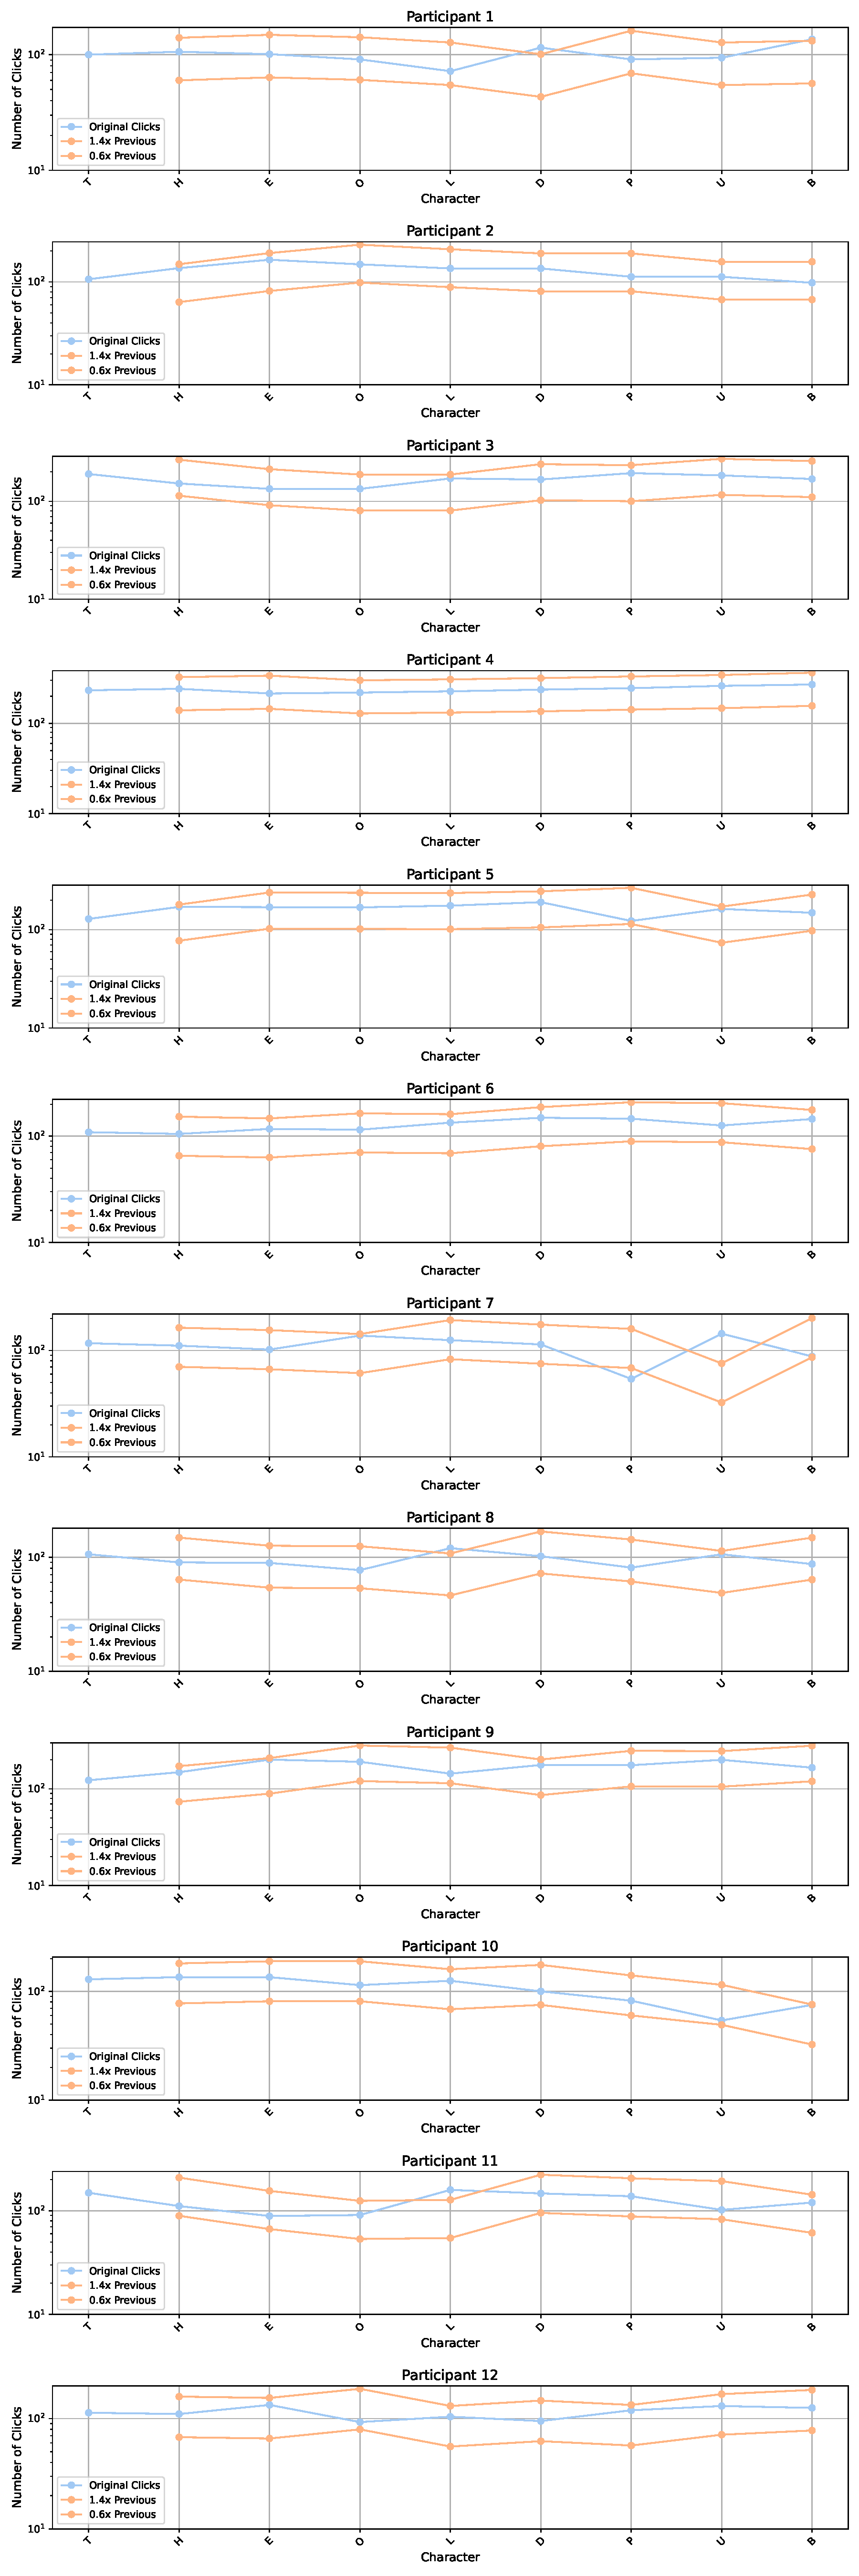
\includegraphics[width=0.5\linewidth]{src/pictures/Study1Data_questionnaire/participantPlots_study1.pdf}
    \caption{Participant Click-differences.}
    \label{fig:participant_clicks-firstStudy}
\end{figure}

In the first study, we interviewed 12 participants (3 female, 9 male), aged between 22 and 55, with an average age of 28.67 and a median age of 27 years. Of these, 11 were right-handed, and one was left-handed, as shown in \autoref{tab:study1_participant_data}. None of the participants had prior knowledge of Braille.

First, we assessed the validity of our data by ensuring that the participants were focused on the game and not on the sensations themselves. To do so, we measured the click rate for each character to detect any differences in performance. Given that participants tended to become more fatigued later in the game, we compared the click rates with those from the previous round to determine whether the data showed a 40\% improvement or decline, as indicated by the two red lines in \autoref{fig:participant_clicks-firstStudy}. As shown, the data passed the test, with the exception of participant 7, where the observed difference can be attributed to the stimulus change and the completion of questionnaires between sessions.


\begin{figure}
    \centering
    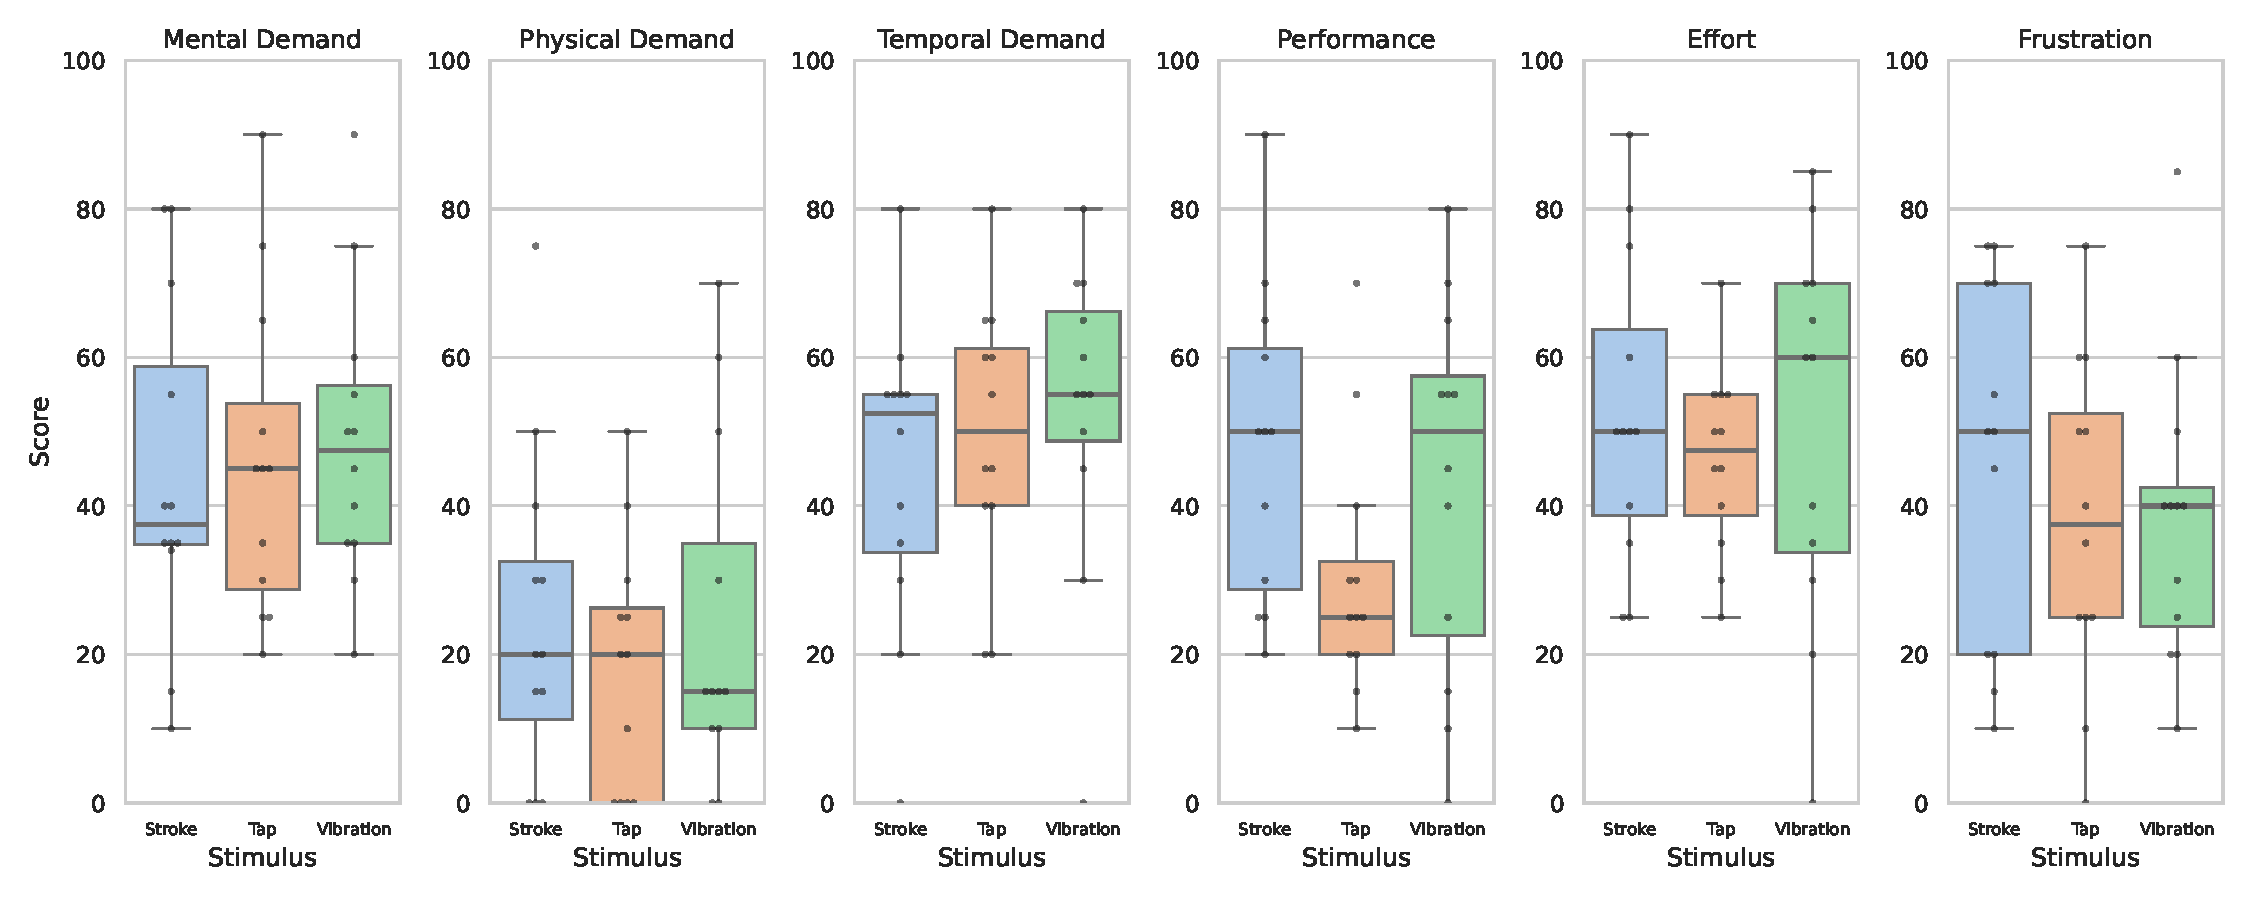
\includegraphics[width=\linewidth]{src/pictures/Study1Data_questionnaire/NasaTLX_study1.pdf}
    \caption{Raw Nasa TLX scores for the different Stimuli grouped by the Nasa TLX dimensions.\\ Each dot represents one participant.}
    \label{fig:nasaTLX-firstStudy}
\end{figure}

The raw NASA-TLX scores are presented in \autoref{fig:nasaTLX-firstStudy}, which displays boxplots for the different stimuli and their corresponding NASA-TLX scores, grouped by the respective NASA-TLX dimensions.

Overall, the medians for the dimensions are similar, with the most notable difference observed in the "performance" dimension. Specifically, the medians are 25.0 for tapping, 50.0 for stroking, and 50.0 for vibration.

In the "physical demand" dimension, a noticeable difference in the quantiles is apparent. The quantile for tapping is slightly larger, indicating that it performed worse on average. Similarly, in the "effort" dimension, slight differences in the quantiles and medians are observed. The medians for stroking and tapping are 50 and 47.5, respectively, while the median for vibration is 60.

In the "frustration" dimension, the quantile range is larger, particularly for the boxplot representing stroking, which has a quantile range of Q1 = 20, Q3 = 70, with a median of 50. In contrast, tapping has a Q1 of 25, Q3 of 55, and a median of 37.5. Vibration shows the smallest quantile range, with a Q1 of 23.5, Q3 of 42.5, and a median of 40.

Subsequently, we tested for significant differences between the sets using Kruskal-Wallis significance tests, the results of which are tabulated in \autoref{table:nasaTLX_significance_firstStudy_nonParam}.
The results indicate no significant differences between the sets, with p-values exceeding the threshold value of $\alpha=0.05$.
The closest p-value to passing the threshold is found in the \enquote{Performance} dimension, with a p-value of 0.1496, which is not close to being statistically significant.




\begin{table}[ht]
\resizebox{\columnwidth}{!}{
\centering
\begin{tabular}{|l|l|l|l|l|}
\hline
\textbf{Question}        & \textbf{H-Statistic}& \textbf{p-value}       & \textbf{Significance}           &\textbf{Effect Size}\\ \hline
\textbf{Mental Demand}    & 0.5311& 0.7668& Not Significant                 &0.0152\\ \hline
\textbf{Physical Demand}  & 0.358& 0.8361                 & Not Significant                 &0.0102\\ \hline
\textbf{Temporal Demand}  & 1.6356& 0.4414& Not Significant                 &0.0467\\ \hline
\textbf{Performance}      & 3.7994& 0.1496& Not Significant                 &0.1086\\ \hline
\textbf{Effort}           & 0.7655& 0.6820& Not Significant                 &0.0219\\ \hline
\textbf{Frustration}      & 0.9098& 0.6345& Not Significant                 &0.0260\\ \hline
\end{tabular}}
\caption{Results of the Kruskal-Wallis significance tests for the different NasaTLX dimensions with a $\eta^2$ Effect Size.}
\label{table:nasaTLX_significance_firstStudy_nonParam}
\end{table}

% Henceforth, with the prerequisites satisfied for almost all of the NASA-TLX dimensions, except for the \enquote{Physical Demand} dimension due to an approximately non-normally distributed dataset (for which we used a Kruskal-Wallis test), we were able to use an ANOVA test for the other dimensions, as shown in \autoref{table:nasaTLX_significance_firstStudy}.
% As seen in the table, the p-values for all the NASA-TLX dimensions are greater than the threshold $\alpha = 0.05$, with the closest value being in the \enquote{performance} dimension, which has a p-value of 0.7342.
% This indicates that there is no statistical significance for any of the dimensions of the NASA-TLX test.





\begin{figure}
    \centering
    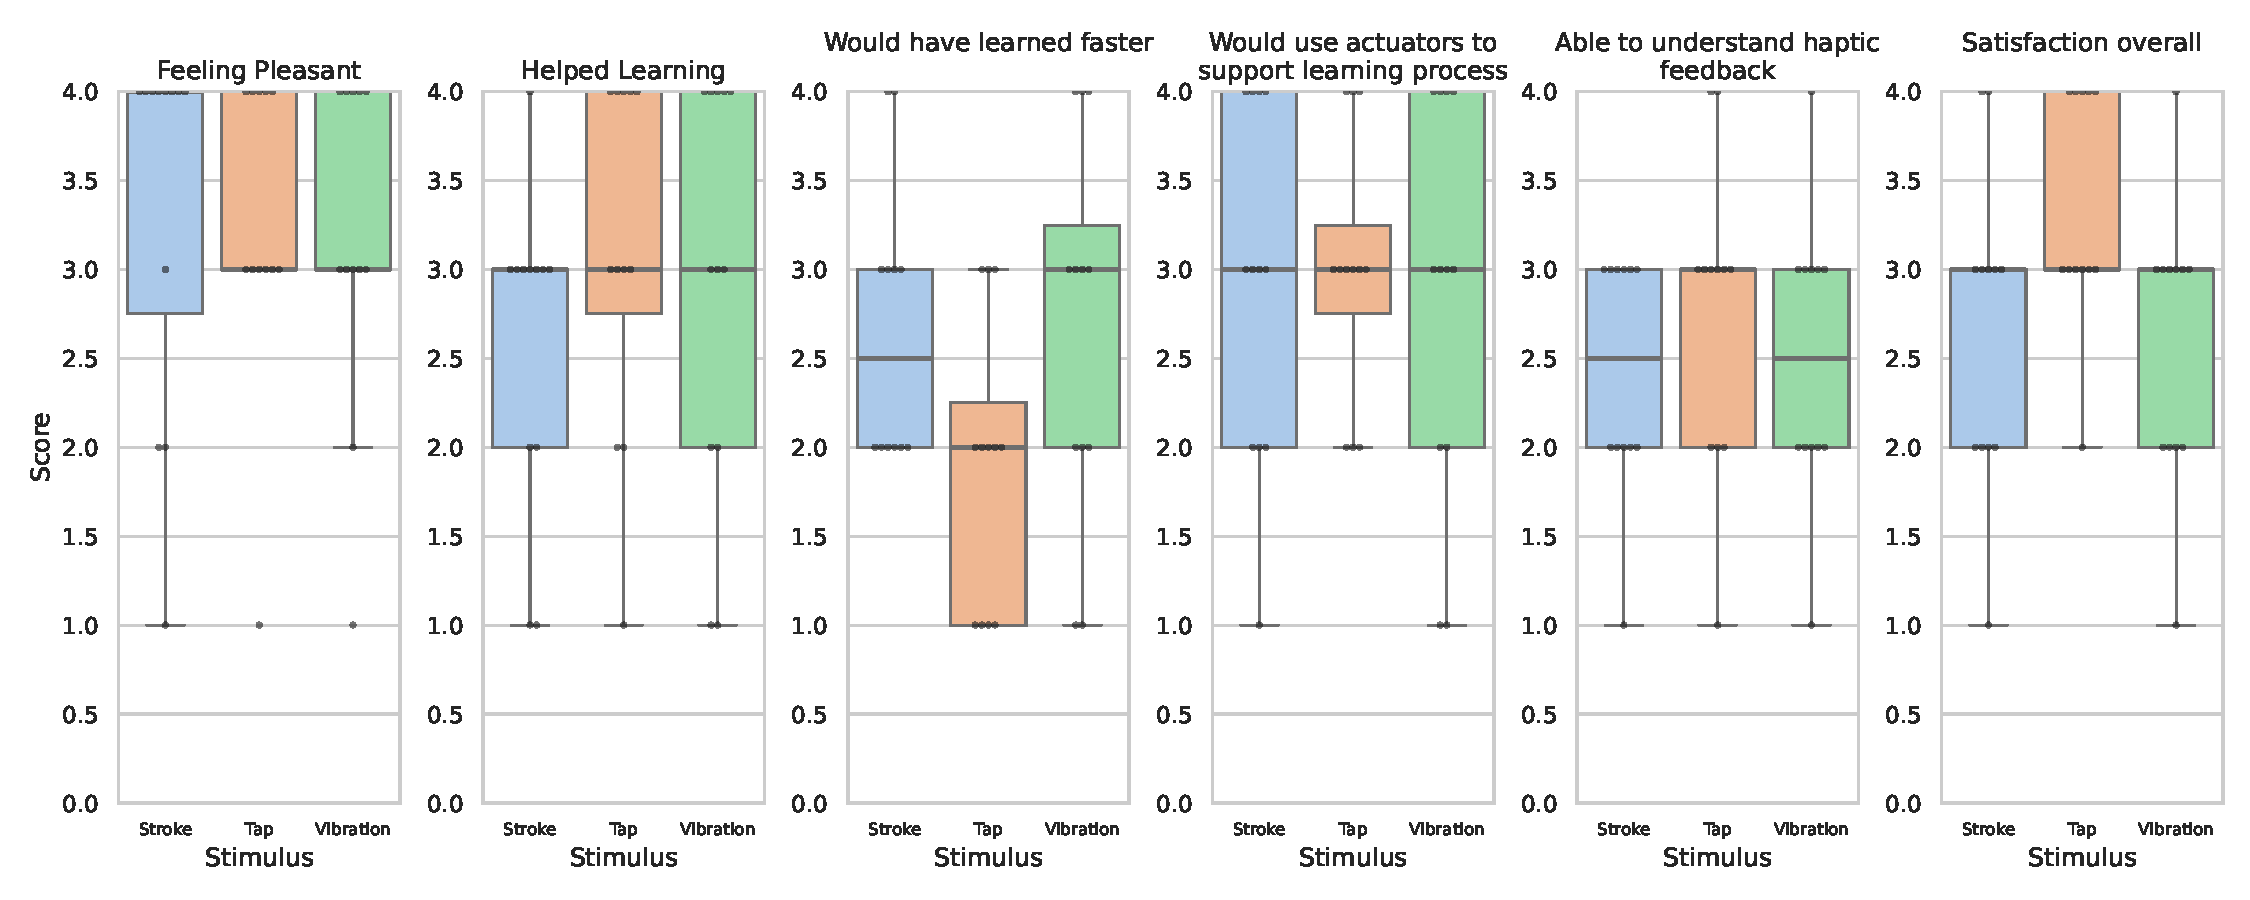
\includegraphics[width=\linewidth]{src/pictures/Study1Data_questionnaire/questions_special_study1.pdf}
    \caption{Self-assessment Results of the different Stimuli grouped by the self-assessment categories.\\4 is the best score and 0 the worst score.\\Each dot represents one participant.}
    \label{fig:questions_individual_firstStudy}
\end{figure}

After the Task Load Index, we surveyed five dimensions to assess how the participants perceived learning and usability with the different actuators, comparing the stimuli across six different dimensions, as shown in \autoref{fig:questions_individual_firstStudy}.

As shown in the figure, there are larger differences in the dimensions \enquote{Helped learning}, \enquote{Would have learned faster}, \enquote{Would use actuators to support the learning process}, and \enquote{Satisfaction overall}.

For the \enquote{Feeling pleasant} dimension, the median values differ by 4 for stroking, and 3 for tapping and vibration. However, the Q1-Q3 quantile ranges are similar, with ranges of 3 to 4 for tapping and vibration, and 2.75 to 4 for stroking. Although the median for stroking is better, there are more outliers for stroking compared to the other two stimuli.

In the \enquote{Helped learning} dimension, the medians are identical for all stimuli, each with a value of 3. However, the quantile ranges differ slightly, with a Q1-Q3 range of 2 to 3 for stroking, 2.75 to 4 for tapping, and 2 to 4 for vibration.

For the \enquote{Would have learned faster} dimension, the medians differ: 2.5 for stroking, 3 for vibration, and 2.0 for tapping, as shown in orange.

In the \enquote{Would use actuators to support the learning process} dimension, the medians are the same for all three stimuli. However, the variance differs considerably, with Q1-Q3 intervals of 2 to 4 for stroking and vibration, while the Q1-Q3 interval for tapping is 2.75 to 3.25.

For \enquote{Satisfaction overall}, the Q1-Q3 intervals are identical for stroking and vibration, ranging from 2 to 3, and from 3 to 4 for tapping. The medians, however, are the same (3.0) for all three stimuli in this dimension.

In the \enquote{Able to understand haptic feedback} dimension, there is no difference in the Q1-Q3 quantile range. However, the medians differ, with 2.5 for stroking and vibration, compared to 3.0 for tapping.


To assess statistical differences, we conducted non-parametric Kruskal-Wallis tests, the results of which are presented in \autoref{table:individualQuestions_significance_firstStudy}.
As shown in the table, no statistically significant differences were found between the stimuli for the dimensions, as the p-values for each Kruskal-Wallis test exceed the threshold value of $\alpha=0.05$.

However, the dimensions closest to the threshold are \enquote{Satisfaction overall} (p-value = 0.0504) and \enquote{Would have learned faster} (p-value = 0.0882). Given their relatively low p-values and \(\eta^2\) effect sizes of 0.1707 and 0.1387 for \enquote{Satisfaction overall} and \enquote{Would have learned faster}, respectively, which are considered large, these dimensions are regarded as \enquote{approaching significance}.


\begin{table}[ht]
\resizebox{\columnwidth}{!}{
\centering
\begin{tabular}{|l|l|l|l|l|}
\hline
\textbf{Question}                              & \textbf{H-statistic}& \textbf{p-value}       & \textbf{Significance}           &\textbf{Effect Size}\\ \hline
\textbf{Feeling Pleasant}                      & 0.706& 0.7026                 & Not Significant                 &0.0202\\ \hline
\textbf{Helped Learning}                       & 1.942& 0.3787                 & Not Significant                 &0.0555\\ \hline
\textbf{Would have learned faster}             & 4.855& 0.0882                 & Not Significant                 &0.1387\\ \hline
\textbf{Would use actuators to support learning process} & 0.038& 0.9812                 & Not Significant                 &0.0011\\ \hline
\textbf{Able to understand haptic feedback}    & 1.241& 0.5377                 & Not Significant                 &0.0355\\ \hline
\textbf{Satisfaction overall}                  & 5.975& 0.0504                 & Not Significant                 &0.1707\\ \hline
\end{tabular}}
\caption{Results of the Kruskal-Wallis significance tests for the different self-assessment dimensions with a $\eta^2$ Effect Size.}
\label{table:individualQuestions_significance_firstStudy}
\end{table}





\begin{figure}
    \centering
    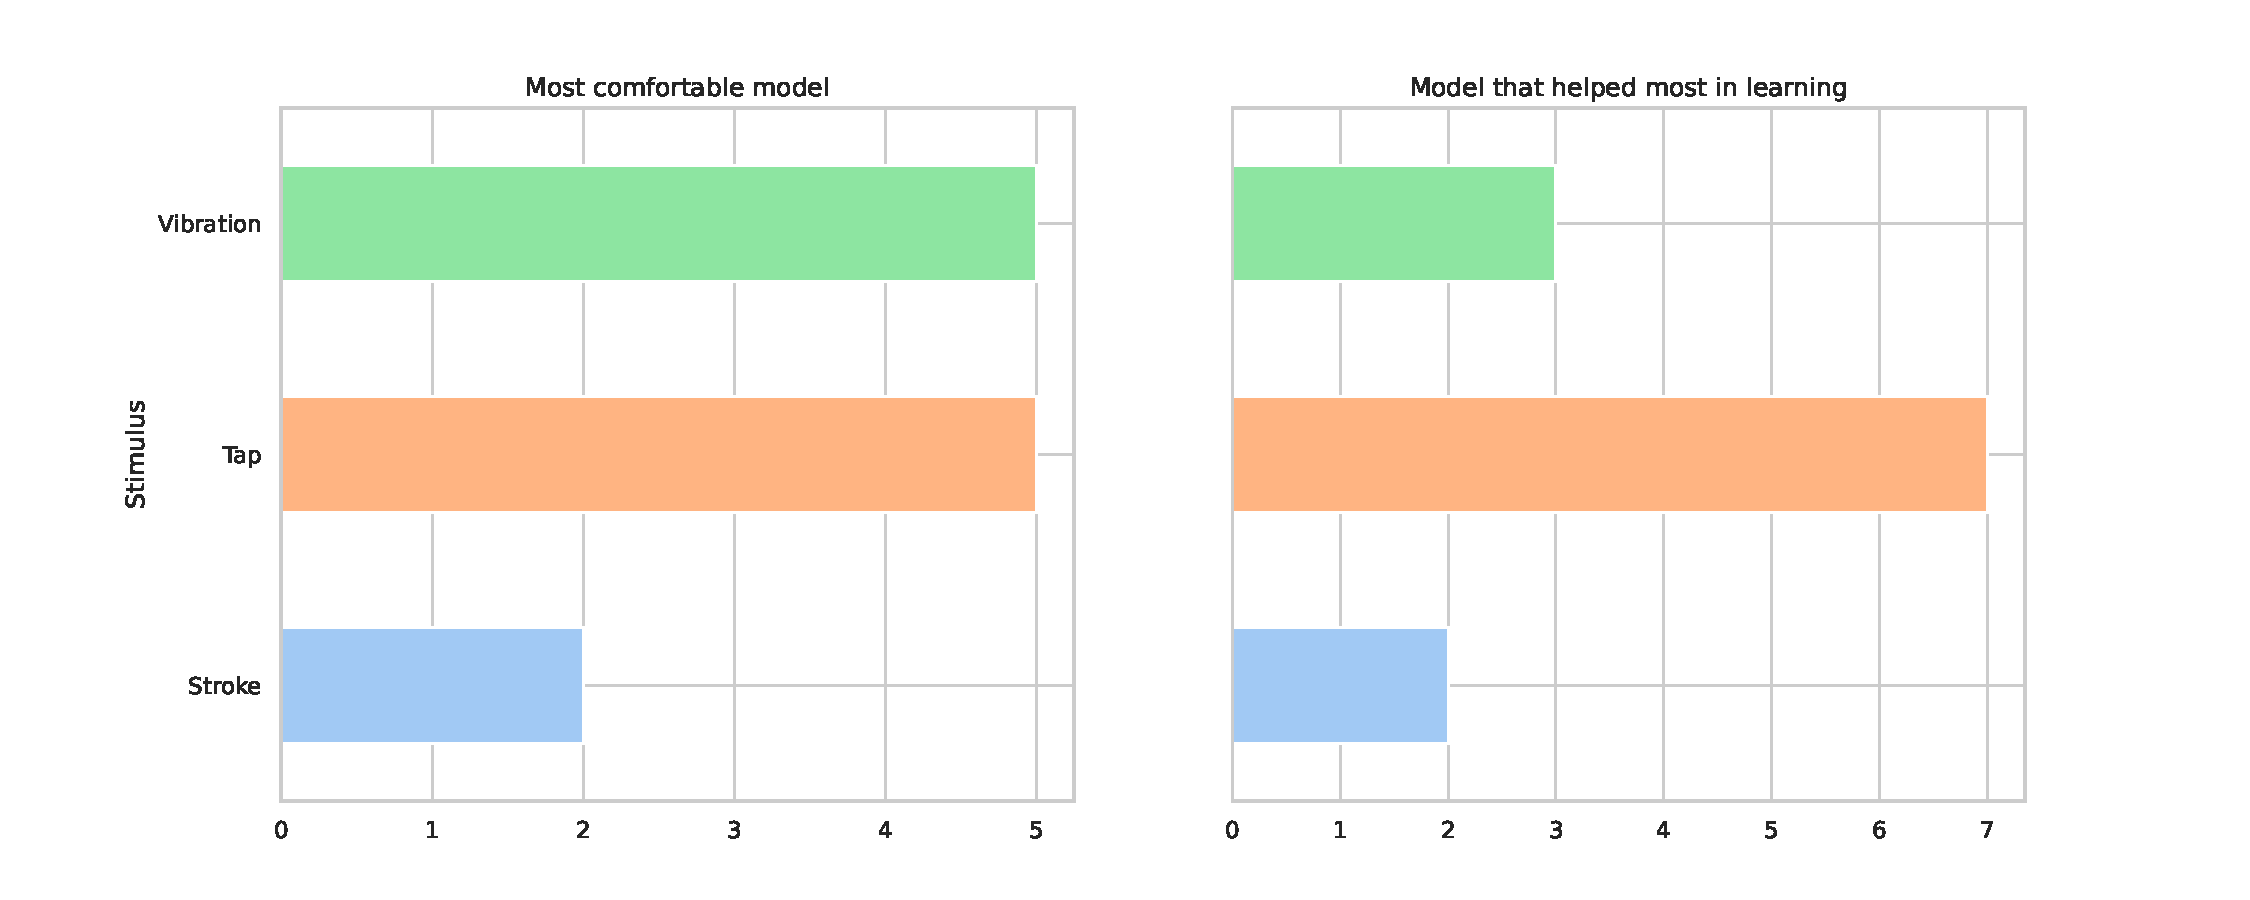
\includegraphics[width=\linewidth]{src/pictures/Study1Data_questionnaire/questions_compare_study1.pdf}
    \caption{Results of the direct comparison between the different stimuli.}
    \label{fig:questionsCompare-firstStudy}
\end{figure}

After completing all the learning sessions for the different stimuli, the participants directly compared the stimuli based on the two dimensions presented in \autoref{fig:questionsCompare-firstStudy}, with the questions \enquote{Which actuator is the most comfortable} on the left and \enquote{Which actuator helped most in learning} on the right. 
$41.67\%$ of the participants found the tapping actuator to be the most comfortable, followed by the vibration actuator, as shown in the left figure, while approximately $16.67\%$ preferred the stroking actuator. This indicates that, according to the participants' judgments, the vibration and tapping actuators were considered superior to the stroking actuators in terms of comfort.

In the \enquote{Which actuator helped most in learning} category, the participants selected the tapping actuator as the most helpful, with $58.33\%$ of participants voting for it, followed by the vibration actuator with $25\%$, and the stroking actuator with $16.67\%$. The stroking actuator was generally perceived as the least effective compared to the other two.

To test for significant statistical differences, we conducted two tests: first, the \gls{csgf}, and, as the sample sizes were relatively small and the expected values might be less than $5$, we performed an additional \gls{emgf}, as suggested by McDonald et al. \cite{mcdonald2014handbook}, because it is likely more accurate. 
The results of these tests are presented in \autoref{table:statistical_tests_comparrisson_firstStudy}. 
As shown, the p-values for the first question, \enquote{Most comfortable model}, are $0.4724$ for the \gls{csgf} and $0.4568$ for the \gls{emgf}, both of which exceed the threshold value of $0.05$. 
The same holds for the question \enquote{Model that helped most in learning}, with p-values of $0.1738$ for the \gls{csgf} and $0.278$ for the \gls{emgf}, indicating that there is no statistically significant difference between the stimuli for those questions.


\begin{table}[ht]
\centering
\resizebox{\columnwidth}{!}{
\begin{tabular}{|l|l|l|l|l|}
\hline
\textbf{Question} & \textbf{Test} & \textbf{Test- Statistic}& \textbf{p-value}  &\textbf{Significance}          \\ \hline
Model most comfortable & \gls{csgf}& 1.5 & 0.4724  &Not Significant                \\
 & \gls{emgf}& 3.464*& 0.4568 &Not Significant                \\\hline
Model that helped most in learning & \gls{csgf}& 3.5 & 0.1738 &Not Significant                \\
 & \gls{emgf}& 4.206*& 0.278 &Not Significant                \\\hline
\end{tabular}}
\caption{Statistical Test Results for the direct comparison between the stimuli.\\\text{*} indicates results obtained via Negative Log-Likelihood under $H_0$.}
\label{table:statistical_tests_comparrisson_firstStudy}
\end{table}

\begin{figure}
    \centering
    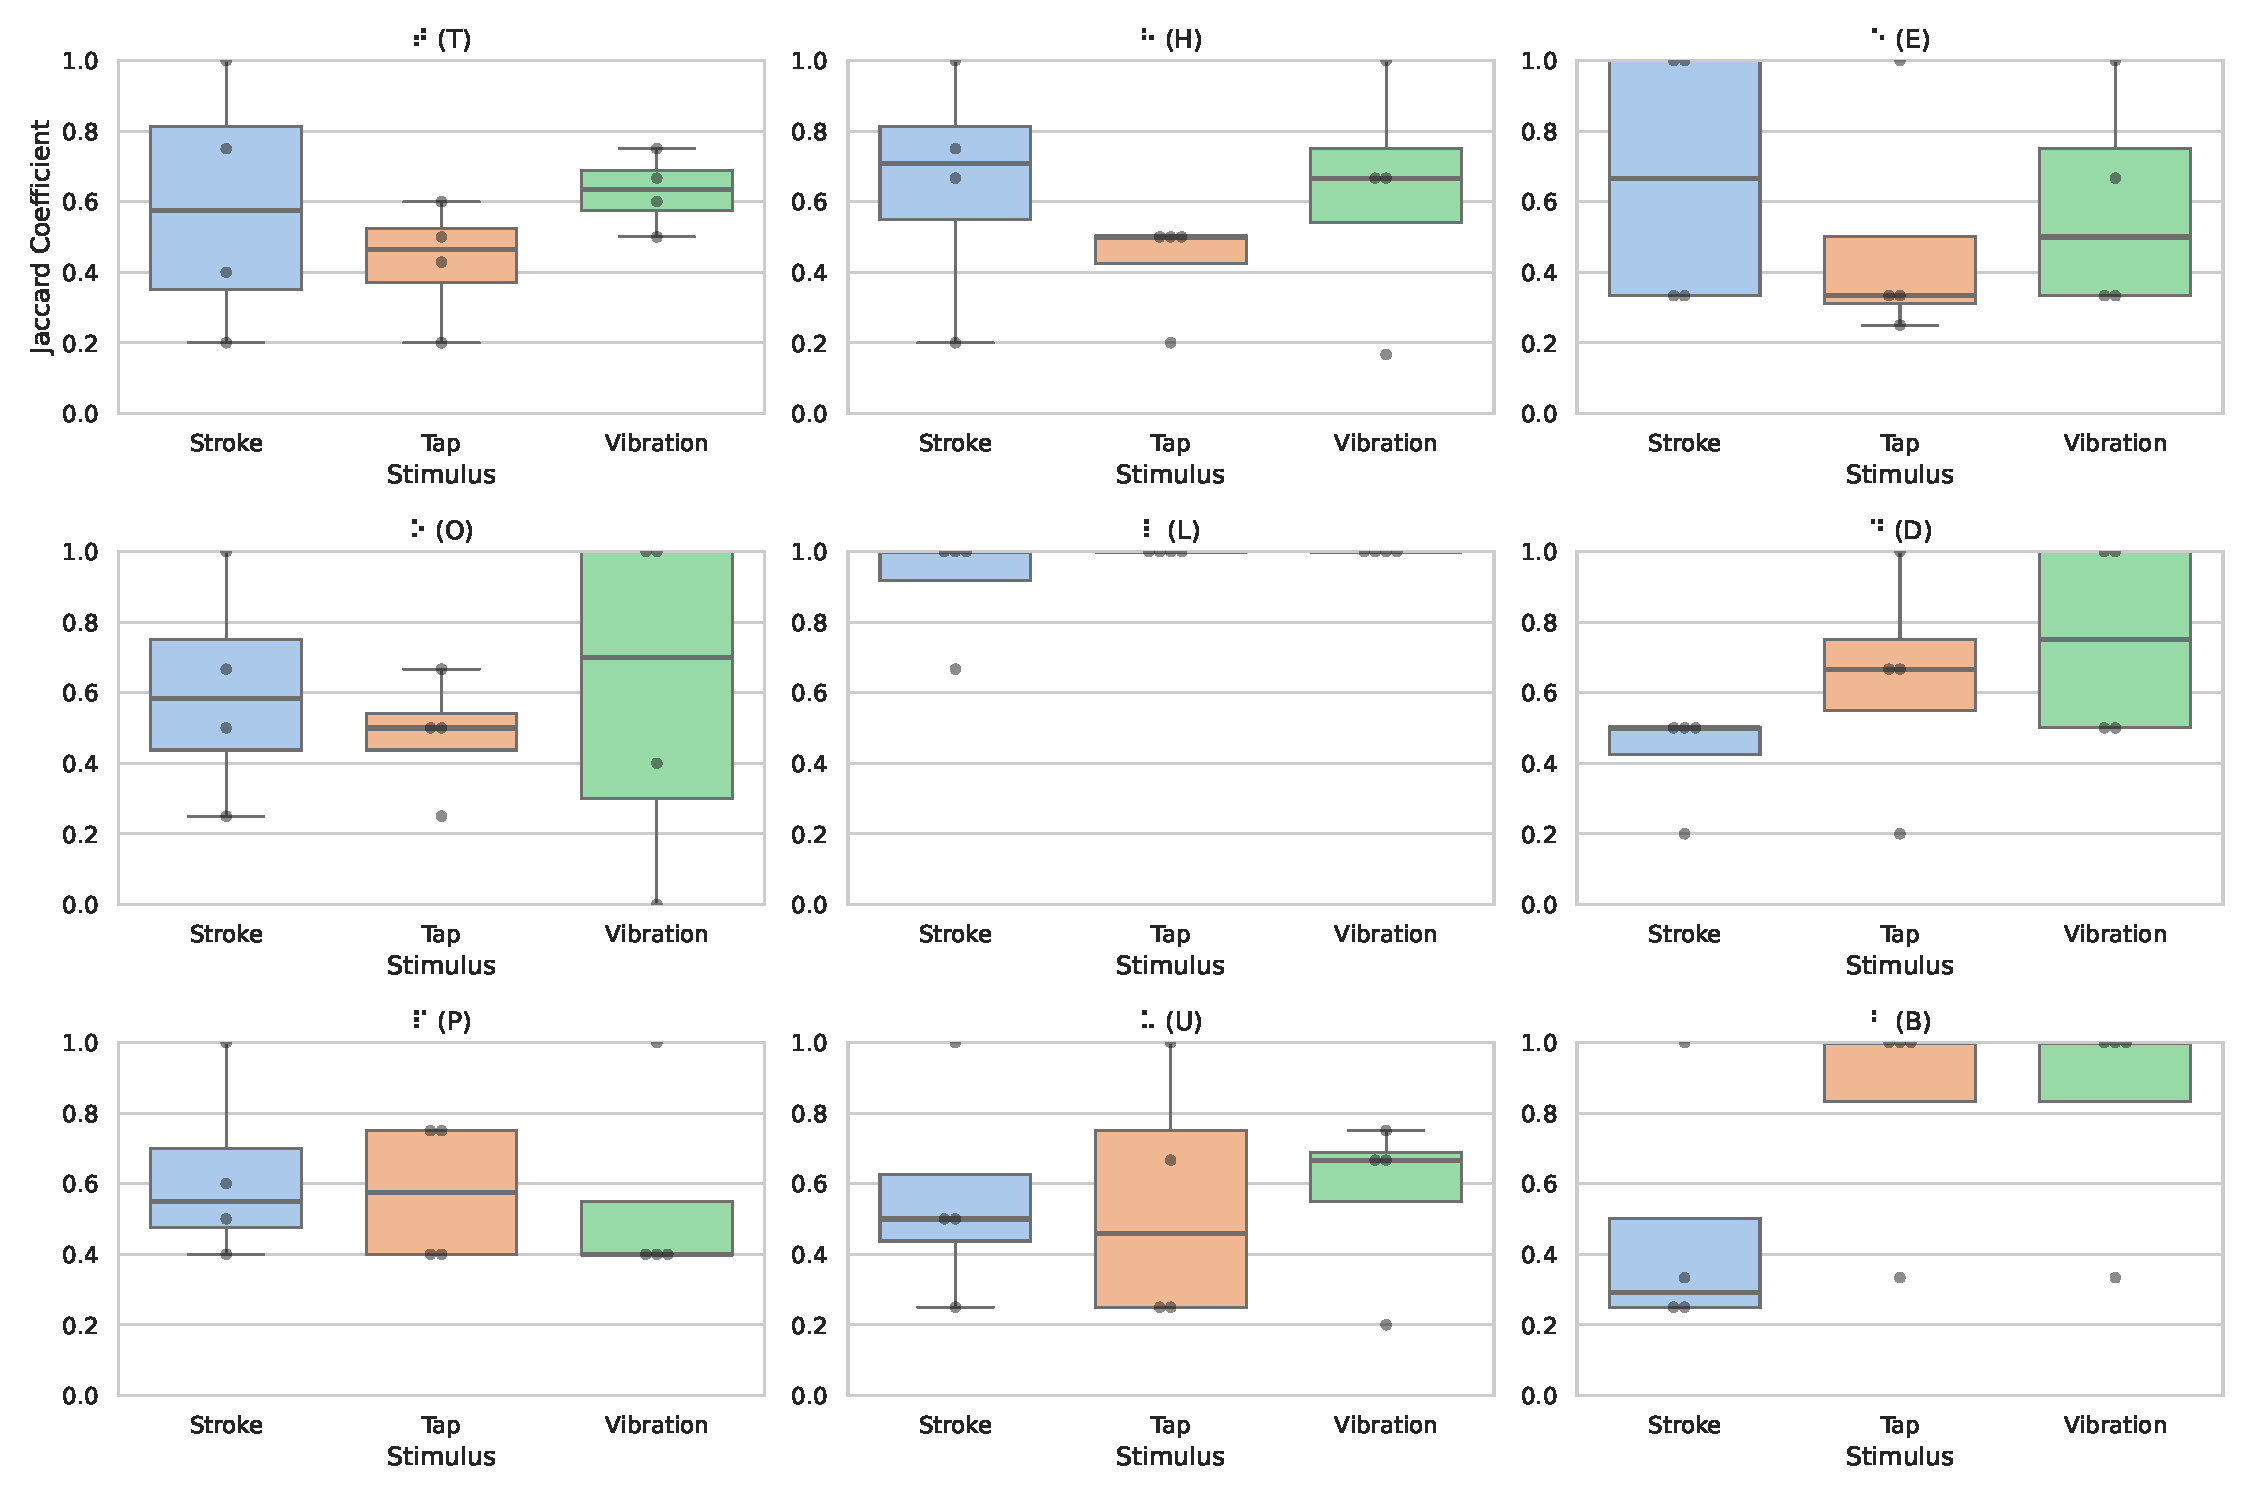
\includegraphics[width=\linewidth]{src/pictures/Study1Data_Experiment/study1_learning_results.pdf}
    \caption{Jaccard coefficient results grouped by the Braille character during learning  for the different stimuli.\\Each dot represents one participant.}
    \label{fig:learning_results_firstStudy}
\end{figure}

After passively learning a character using a specific stimulus, a test was conducted to assess the performance of the characters immediately following the learning session. 
The test results are shown in \autoref{fig:learning_results_firstStudy}, where the stimuli are plotted with their respective Jaccard indices, grouped by the specific characters learned in the session.

The most significant difference is observed for the character \braille{b}(B), where the median for stroking is 0.3, while the medians for tapping and vibration are 1. The quantile ranges for tapping and vibration are 0.82 to 1, while the quantile range for stroking is 0.25 to 0.5.

A similar trend is observed for the character \braille{l}(L), where both tapping and vibration perform perfectly while stroking has an outlier at 0.675. However, all medians are the same at 1.

For the character \braille{h}(H), a larger difference is evident between tapping and the other two stimuli. While tapping has a median of 0.5, the medians for the other two stimuli are approximately 0.7. All three stimuli had a poor outlier, with a score of 0.2.

Another notable difference in medians appears for the character \braille{d}(D), where the median for stroking is 0.5, compared to medians of 0.675 for tapping and 0.75 for vibration. Additionally, the quantile ranges differ: vibration has the largest range, from 0.5 to 1, due to two participants scoring 0.5 and 1, respectively. In contrast, only one participant achieved a perfect score for tapping, and both tapping and stroking have worse participant scores of 0.2.

A further difference can be observed for the character \braille{t}(T), where the median for stroking is approximately 0.6, 0.65 for vibration, and 0.475 for tapping.

To test for significance, we used the Kruskal-Wallis tests. The results, however, did not show any significant differences, as depicted in \autoref{table:learning_significance_results_firstStudy_nonParam}. 
As shown in the \enquote{p-value} column, all p-values for the tests exceed the threshold value of $\alpha = 0.05$, indicating no statistically significant difference between the Jaccard index results of the stimuli for any of the characters.


\begin{table}[ht]
\resizebox{\columnwidth}{!}{
\centering
\begin{tabular}{|l|l|l|l|l|}
\hline
\textbf{Question} & \textbf{Test Statistic} & \textbf{p-value}  &\textbf{Significance}           &\textbf{Effect Size}\\ \hline
\braille{t}(\textbf{T})& 1.9406 & 0.3790  &Not Significant &0.1764\\ \hline
\braille{h}(\textbf{H})& 2.2817& 0.3195&Not Significant &0.2074\\ \hline
\braille{e}(\textbf{E})& 1.1068 & 0.5750  &Not Significant &0.1006\\ \hline
\braille{o}(\textbf{O})& 0.2790& 0.8698&Not Significant &0.0254\\ \hline
\braille{l}(\textbf{L})& 2.0000 & 0.3679  &Not Significant &0.1818\\ \hline
\braille{d}(\textbf{D})& 2.9298& 0.2311&Not Significant &0.2663\\ \hline
\braille{p}(\textbf{P})& 0.7068 & 0.7023  &Not Significant &0.0643\\ \hline
\braille{u}(\textbf{U})& 0.0299& 0.9852&Not Significant &0.0027\\ \hline
\braille{b}(\textbf{B})& 3.6667 & 0.1599  &Not Significant &0.3333\\ \hline
\end{tabular}}
\caption{Results of Kruskal-Wallis significance tests for the different Braille characters during learning with a $\eta^2$ Effect Size.}
\label{table:learning_significance_results_firstStudy_nonParam}
\end{table}



\begin{figure}
    \centering
    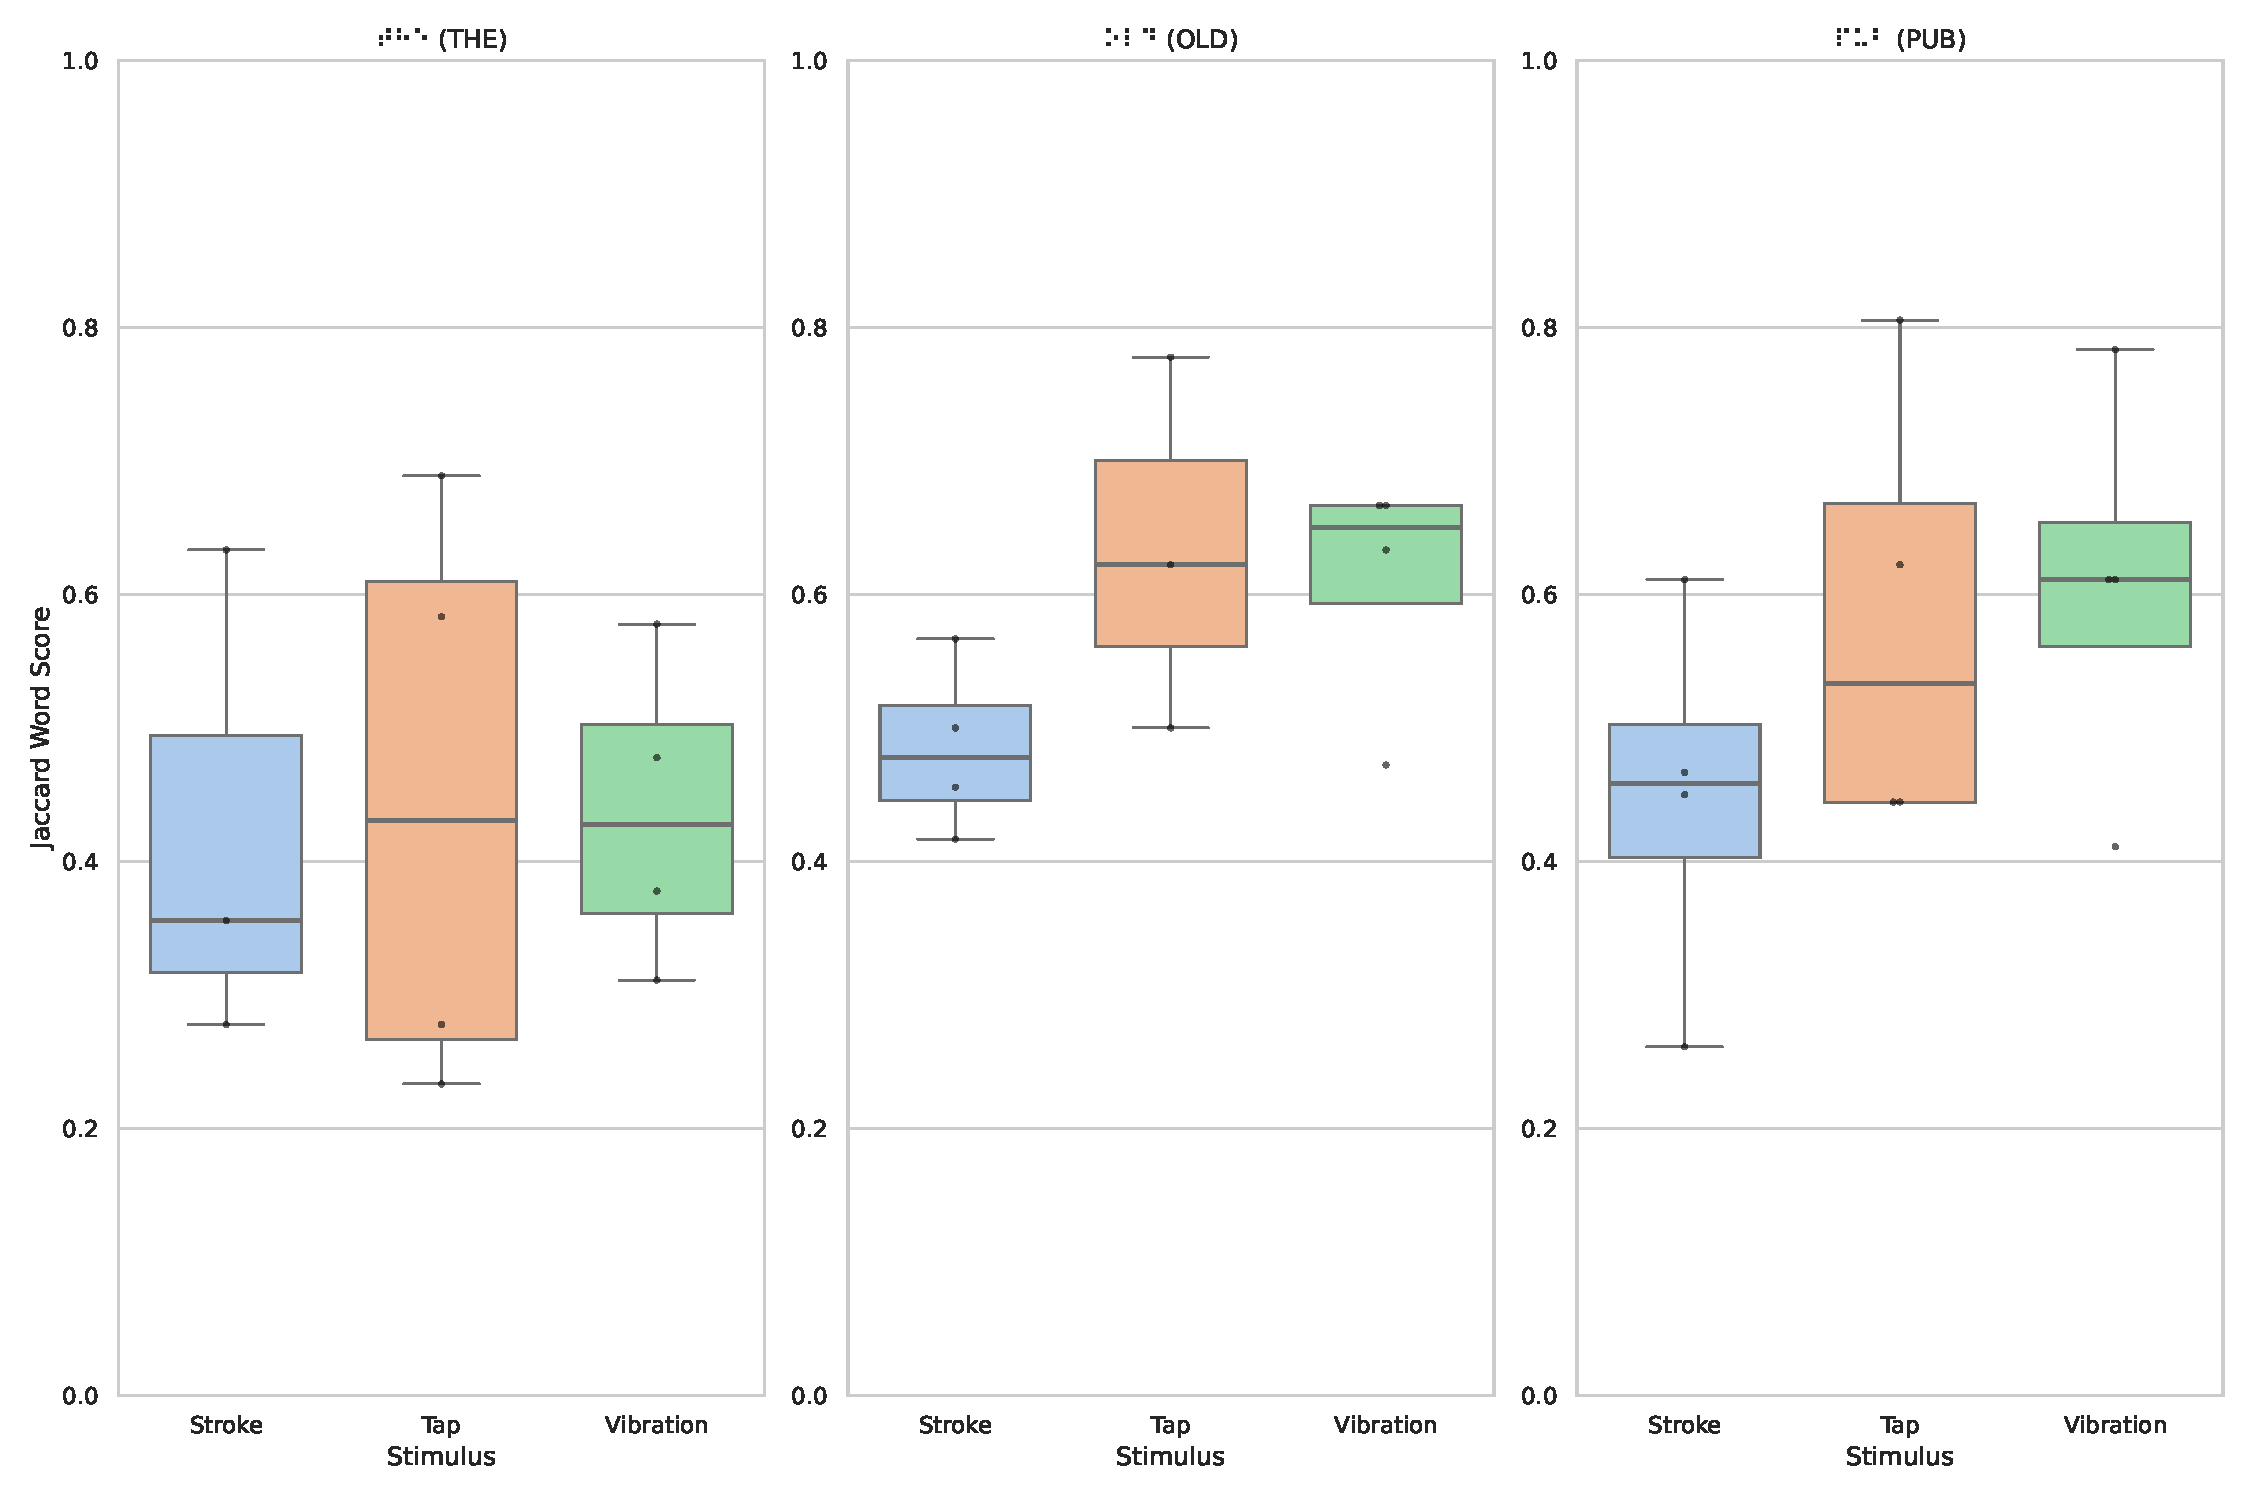
\includegraphics[width=\linewidth]{src/pictures/Study1Data_Experiment/study1_test_results.pdf}
    \caption{Jaccard Word-Test results grouped by the results for the Braille test-words\\
    \enquote{THE}, \enquote{OLD} and \enquote{PUB} for different stimuli.}
    \label{fig:test_results_firstStudy}
\end{figure}



After the passive learning sessions for all characters using a single stimulus, we conducted a word test for the characters learned during the previous passive learning sessions with that stimulus. 
The Jaccard score results, compared across the stimuli for each word, are depicted in \autoref{fig:test_results_firstStudy}. 
As shown, the differences in performance are smaller than those observed for the individual characters. 

For the word \braille{the}(THE), the medians are 0.375 for stroking, 0.425 for tapping, and 0.425 for vibration. The quantile ranges are 0.35-0.5 for stroking, 0.3-0.6 for tapping, and 0.475-0.45 for vibration, respectively.

For the word \braille{old}(OLD), the medians are 0.62 for tapping and 0.625 for vibration, compared to 0.475 for stroking.

For the word \braille{pub}(PUB), the median for stroking (0.45) is somewhat lower than that for tapping (0.56) and vibration (0.61). 

Additionally, it can be observed that the quantile range for tapping is almost twice as large as that of the other two stimuli, with an approximate range of 0.2 compared to 0.1 for both vibration and stroking.

To test for significance, we performed a Kruskal-Wallis test, the results of which are depicted in \autoref{table:significance_results_test_firstStudy}. 
The results showed that all p-values are well above the threshold $\alpha$, with the closest value being 0.1371 for the word \braille{old}(OLD). 
This indicates that there was no statistically significant difference between the Jaccard index results for the different stimuli in relation to the word tests.

\begin{table}[ht]
\resizebox{\columnwidth}{!}{
\centering
\begin{tabular}{|l|l|l|l|l|}
\hline
\textbf{Question} & \textbf{Test Statistic} & \textbf{p-value}  &\textbf{Significance}           &\textbf{Effect Size}\\ \hline
\braille{the}(\textbf{THE})& 0.0361& 0.9821&Not Significant &0.0036\\ \hline
\braille{old}(\textbf{OLD})& 3.9736 & 0.1371  &Not Significant &0.1371\\ \hline
\braille{pub}(\textbf{PUB})& 1.0569& 0.5895&Not Significant &0.0961\\ \hline
\end{tabular}}
\caption{Results of the Kruskal-Wallis significance tests for the wordtests \enquote{THE}, \enquote{OLD}, and \enquote{PUB} with a $\eta^2$ Effect Size.}
\label{table:significance_results_test_firstStudy}
\end{table}



\begin{figure}
    \centering
    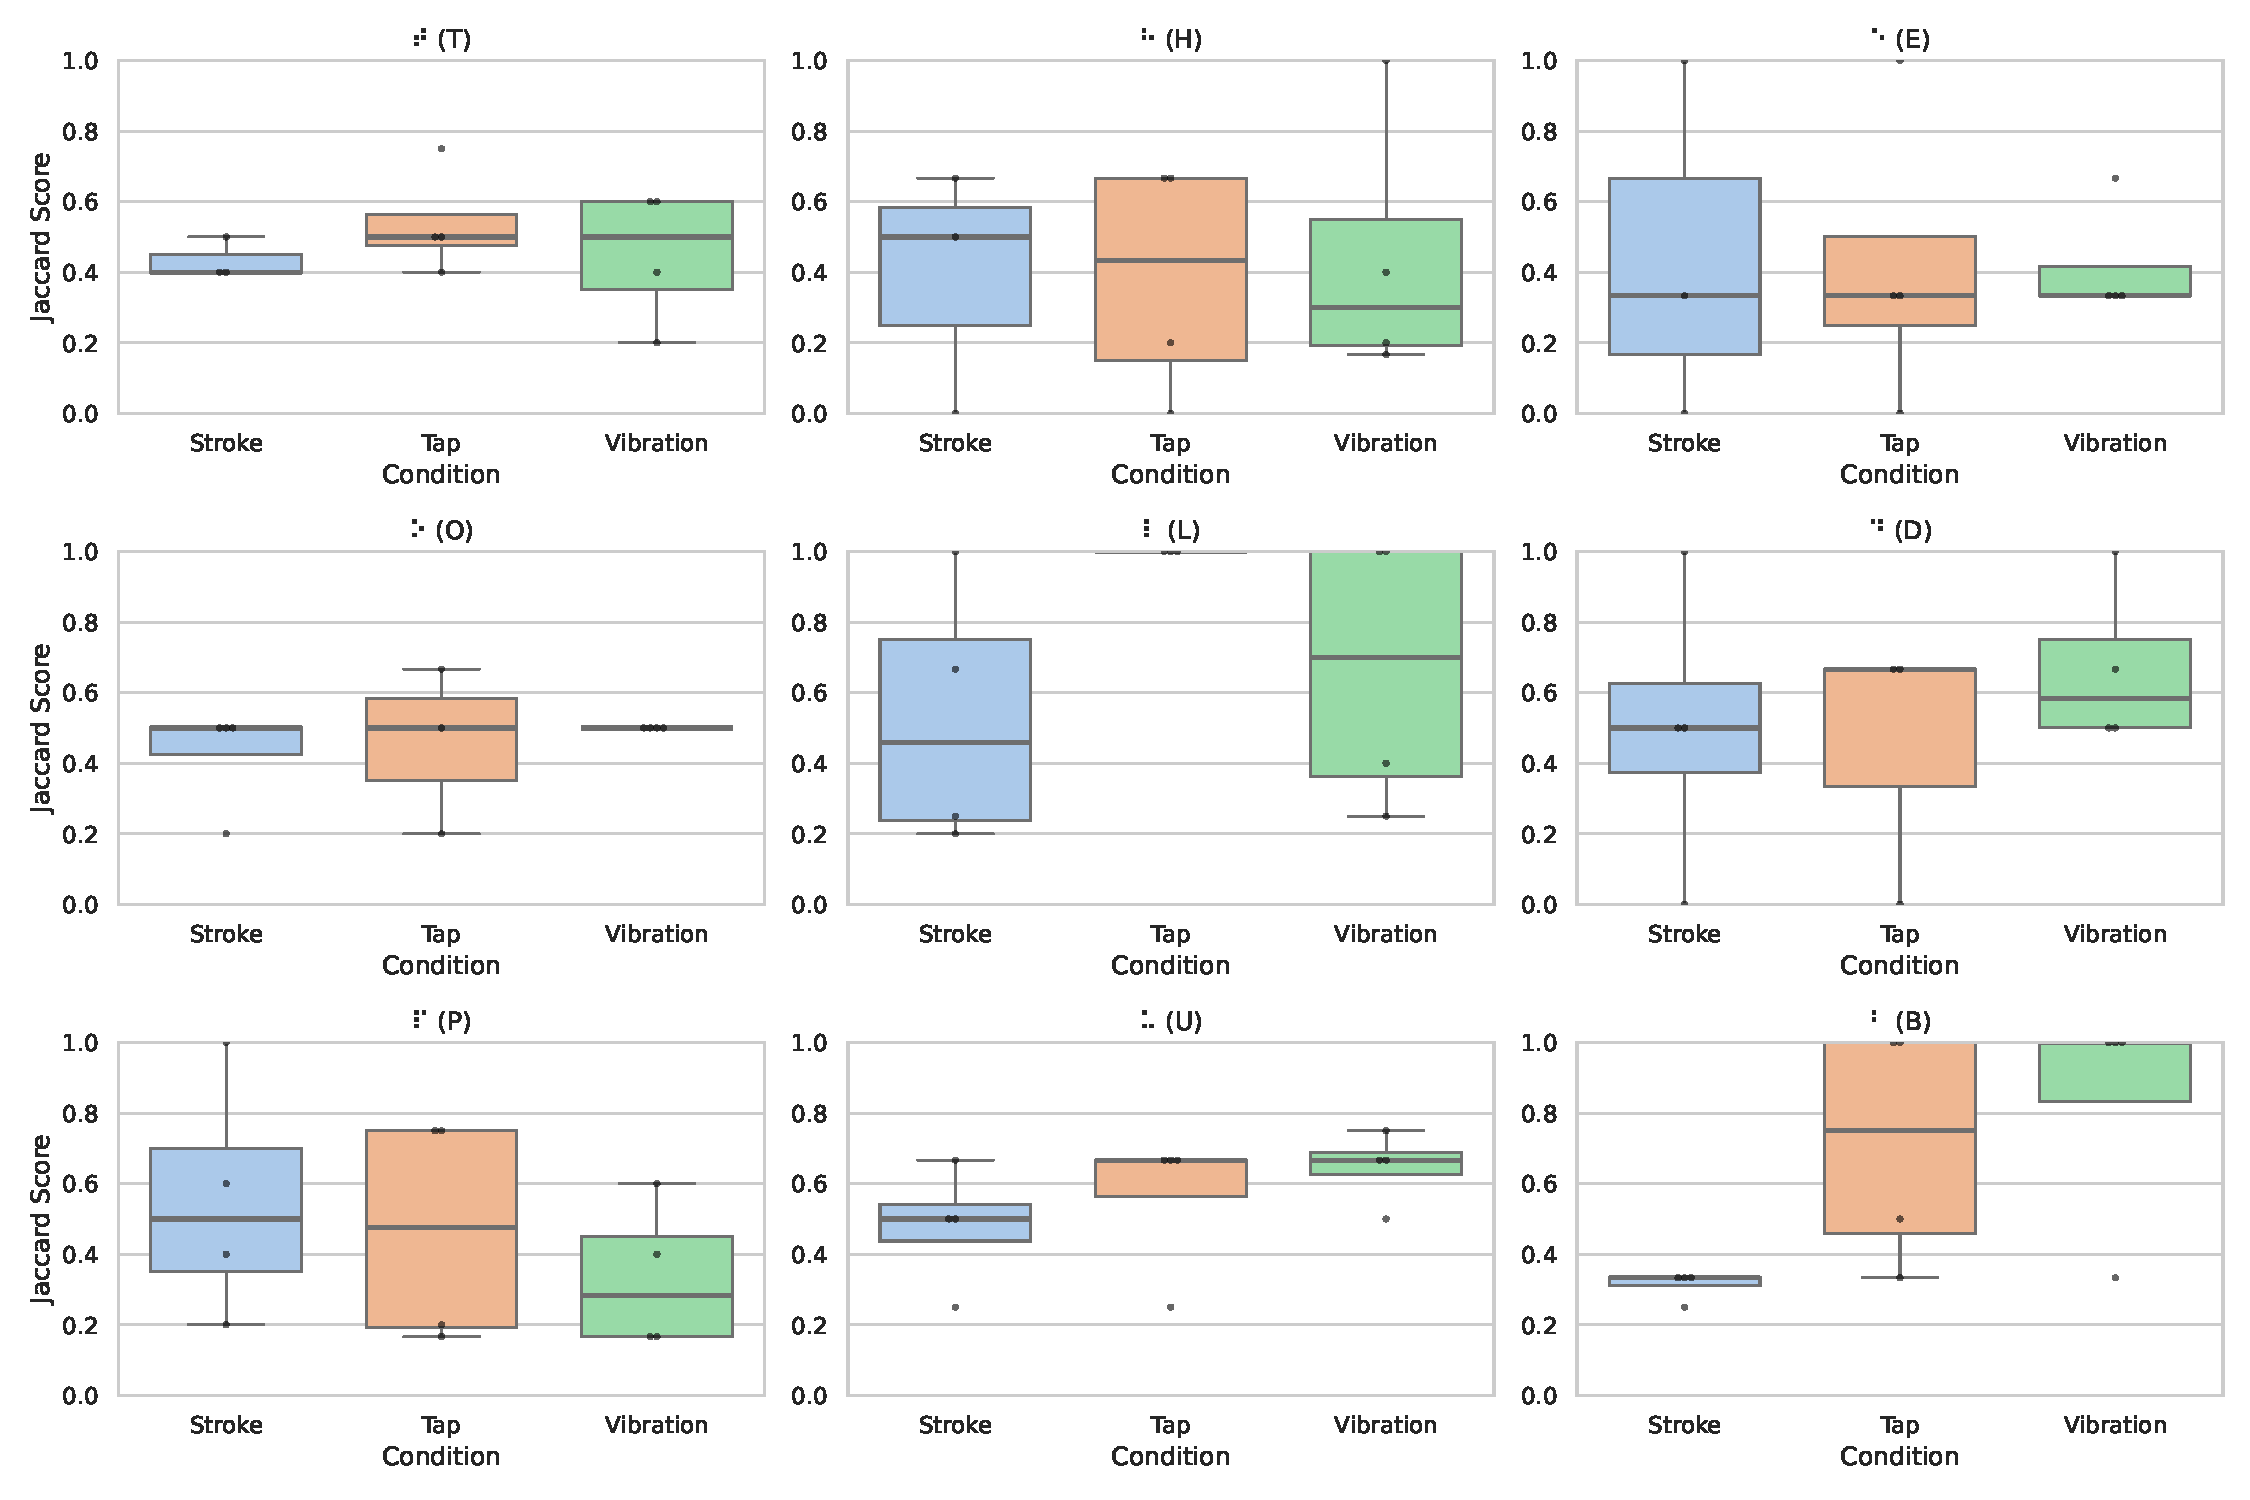
\includegraphics[width=\linewidth]{src/pictures/Study1Data_Experiment/character_jaccard_test_study1.pdf}
    \caption{Jaccard Score comparison for the different Stimuli grouped by the Braille test-word characters.}
    \label{fig:jaccard_test_study1}
\end{figure}


We further investigated the results by breaking them down for each individual character and analyzing them by examining false positives and false negatives in the construction of the Jaccard score. 
We regarded the decision to press a key or not as a classification task. 
Thus, a "missed character" is classified as a false negative, and a "surplus character" is classified as a false positive. 
Using this approach, we calculated precision and recall to derive the Jaccard score. 
These values are plotted in \autoref{fig:jaccard_test_study1}. 

As shown in the plot, the Jaccard score values do not differ significantly across most of the boxplots. 
The largest differences are observed for the character \braille{l}(L), where tapping performed the best with a median of 1 while stroking performed the worst with a median of 0.45 and vibration had a median of 0.7. 
Although perfect scores are observed for all stimuli, stroking had more low data points, with Jaccard scores of 0.2 and 0.25.

The character \braille{b}(B) showed a different pattern, with a median of approximately 0.325 for stroking, 0.75 for tapping, and 1 for vibration. 
None of the stroking participants were able to press the correct keys, whereas 2 participants in the tapping condition and 3 in the vibration condition succeeded in learning the character.

Additional differences were noted for the characters \braille{d}(D) and \braille{p}(P). 
For \braille{p}(P), the median for stroking was higher than the other stimuli, with a median of 0.5 compared to 0.45 for tapping and 0.3 for vibration. 

For \braille{d}(D), stroking was the worst-performing stimulus, with a median of 0.5 compared to 0.6 for tapping and 0.58 for vibration. 
It is important to note that there was only one perfect score for both vibration and stroking, while there were also scores of 0 for both stroking and tapping.

However, when testing for statistical significance using Kruskal-Wallis tests, which are tabulated in \autoref{table:learning_significance_results_firstStudy_nonParam}, no significant differences were found for any stimulus across the characters, with the exception of \braille{b}(B), which approached significance with a p-value of 0.0559 and a large \(\eta^2\) effect size of 0.3906.


\begin{table}[ht]
\resizebox{\columnwidth}{!}{
\centering
\begin{tabular}{|l|l|l|l|l|}
\hline
\textbf{Question} & \textbf{Test Statistic} & \textbf{p-value}  &\textbf{Significance}           &\textbf{Effect Size}\\ \hline
\braille{t}(\textbf{T})& 1.0203& 0.6004&Not Significant &0.1131\\ \hline
\braille{h}(\textbf{H})& 0.0136& 0.9932&Not Significant &0.0017\\ \hline
\braille{e}(\textbf{E})& 0.0979& 0.9522&Not Significant &0.0121\\ \hline
\braille{o}(\textbf{O})& 0.5309& 0.7669&Not Significant &0.0622\\ \hline
\braille{l}(\textbf{L})& 3.3764& 0.1849&Not Significant &0.2968\\ \hline
\braille{d}(\textbf{D})& 0.5290& 0.7676&Not Significant &0.0620\\ \hline
\braille{p}(\textbf{P})& 1.6124& 0.4465&Not Significant &0.1519\\ \hline
\braille{u}(\textbf{U})& 2.5488& 0.2796&Not Significant &0.2207\\ \hline
\braille{b}(\textbf{B})& 5.7683& 0.0559&Not Significant &0.3906\\ \hline
\end{tabular}}
\caption{Results of Kruskal-Wallis significance tests for the different Braille characters during testing with a $\eta^2$ Effect Size.}
\label{table:learning_significance_results_firstStudy_nonParam}
\end{table}





\begin{figure}
    \centering
    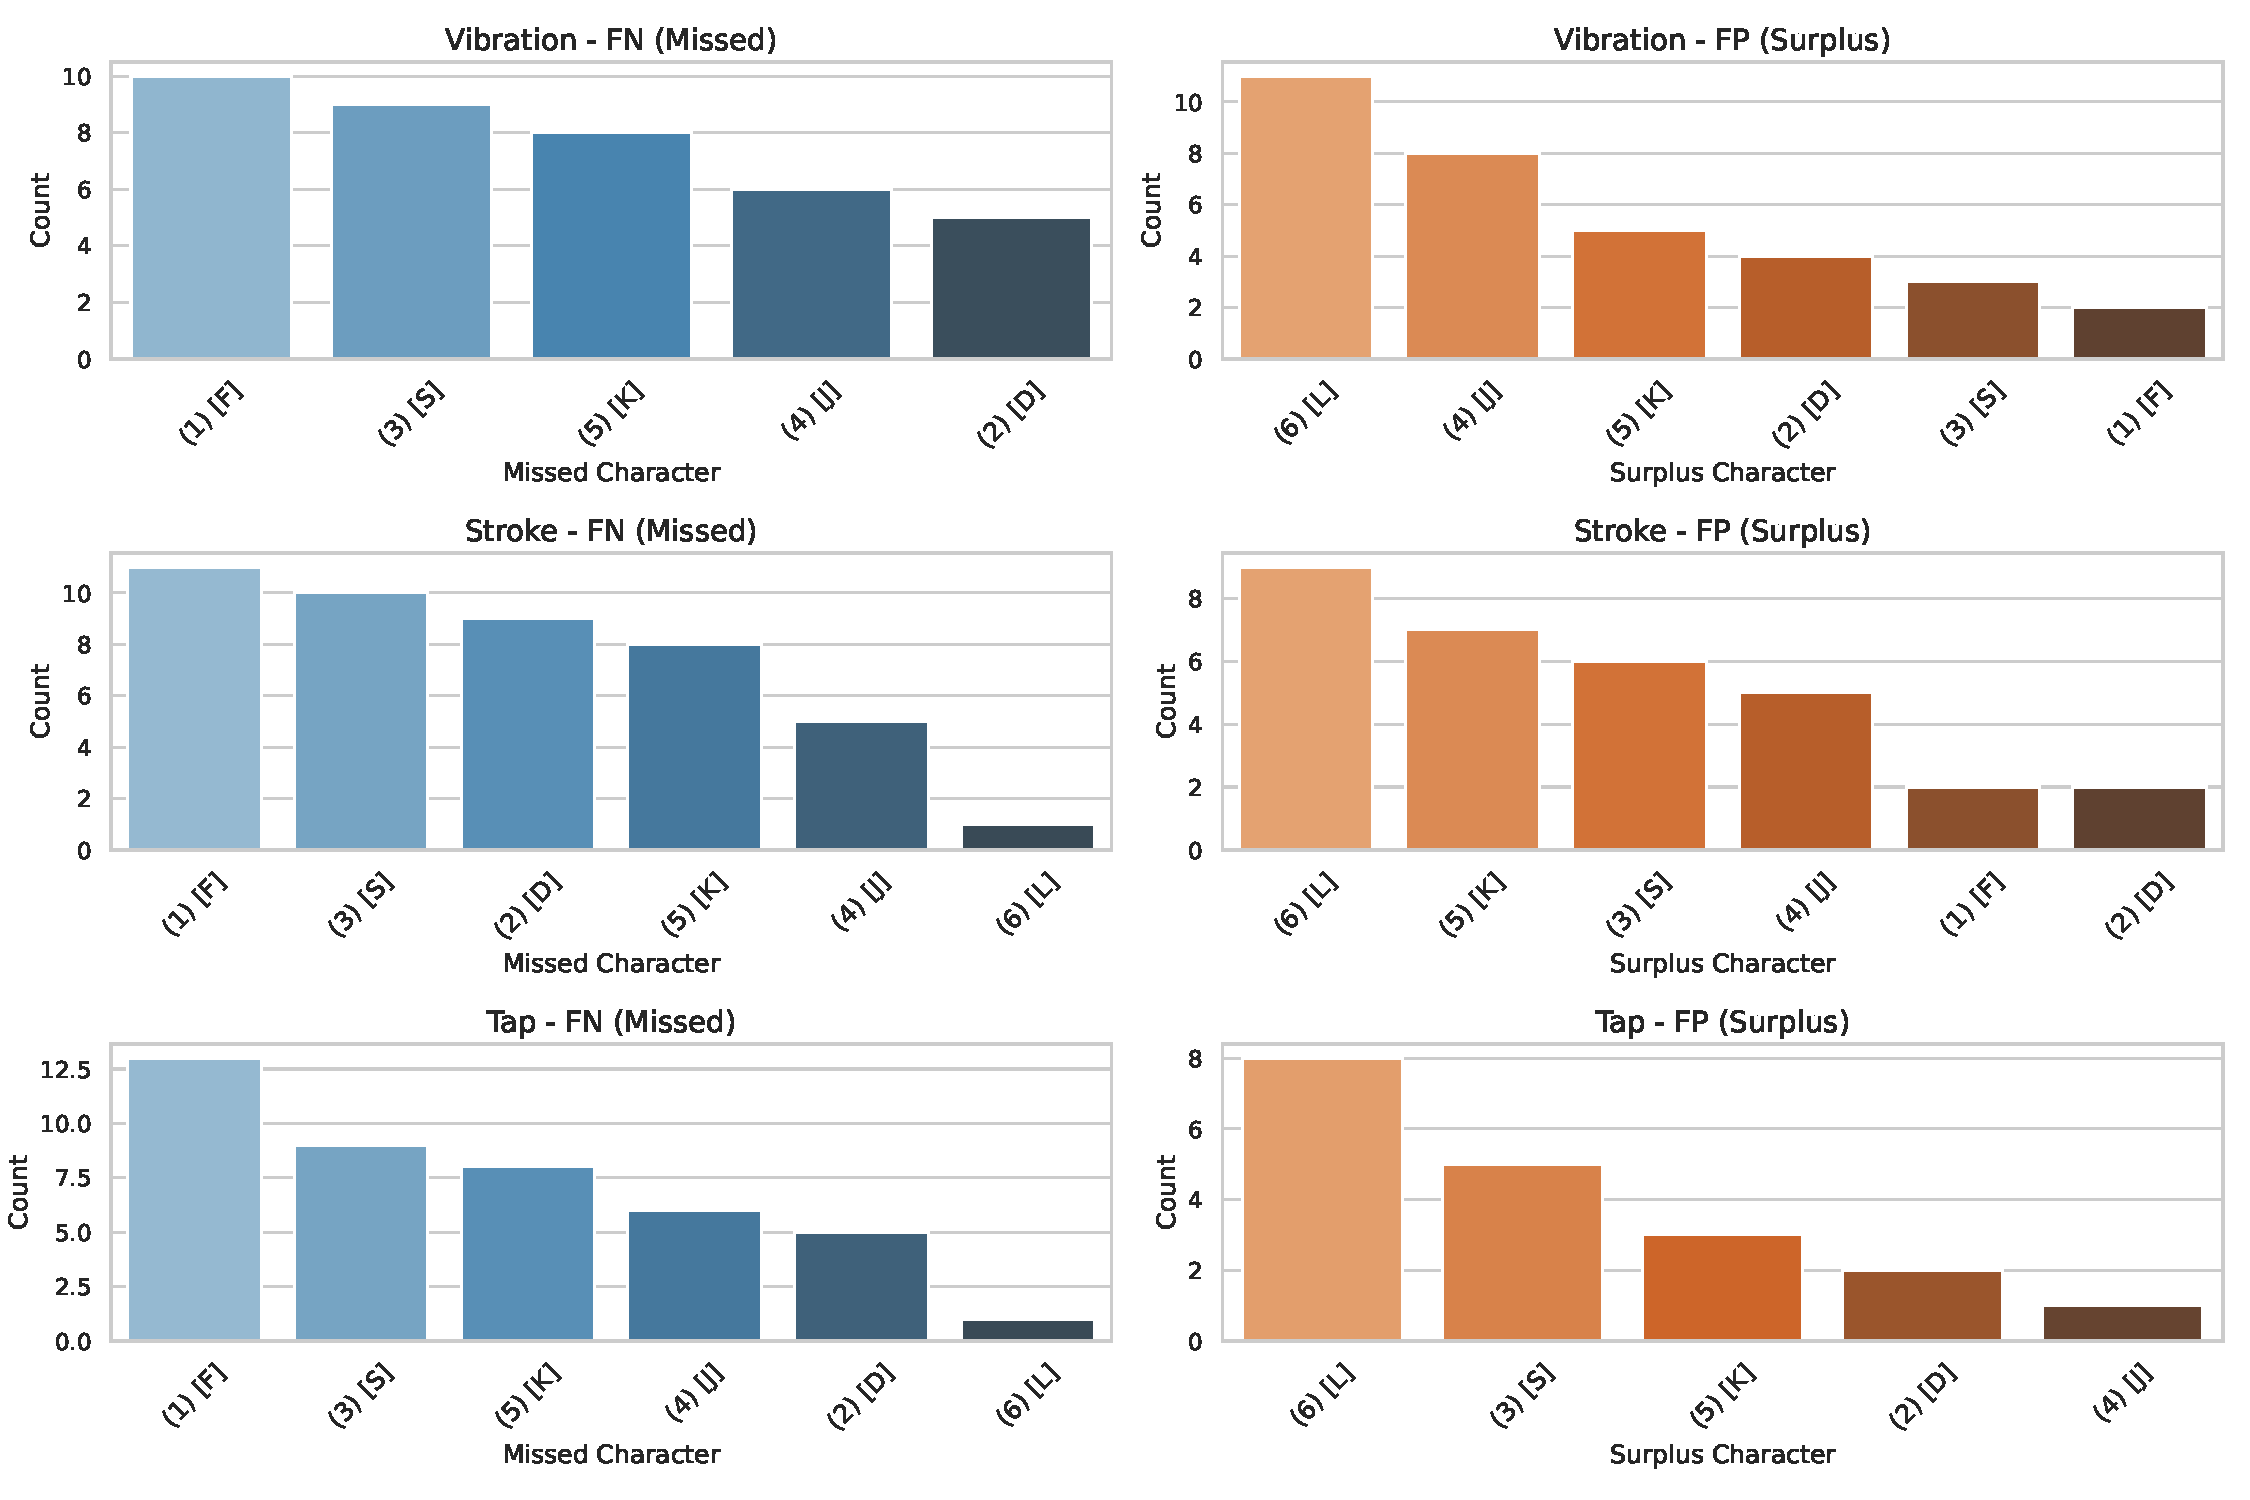
\includegraphics[width=\linewidth]{src/pictures/Study1Data_Experiment/missed_surplus_test_study1.pdf}
    \caption{FN  (Missed) and FP (Surplus) key(s) for each stimuli.}
    \label{fig:missedSurplus_study1}
\end{figure}

To analyse the data that contributed to the Jaccard scores previously presented, we further examined the missed and surplus characters—those that were either missed or incorrectly submitted in addition to the required characters during the test. 
The results for the missed and surplus characters are depicted in \autoref{fig:missedSurplus_study1}, grouped by the stimulus.

As shown for the false negative characters (missed characters), marked in blue on the left side, the first two missed characters are always \textcircled{1} [F] and \textcircled{3} [S], followed by \textcircled{4} [K] for both the vibration and tapping stimuli. 
For the stroking stimulus, \textcircled{2} [D] follows, and then \textcircled{4} [K]. 
The character \textcircled{6} [L] was the least missed, as it does not appear among the missed characters for the vibration stimulus and ranks last for both the stroking and tapping stimuli. 
Next, the character \textcircled{2} [D] appears, which is ranked last for vibration and second-to-last for tapping. 
Following this, \textcircled{4} [J] is the second-to-last missed character for the vibration and stroking stimuli, and ranks third from the bottom for the tapping stimulus.

For the false positives (surplus characters), shown in red on the right, the most frequently added character is \textcircled{6} [L]. 
This indicates that, in most cases, the character \textcircled{6} [L] was added too often. However, the specific differences between the actuators vary. 
The \textcircled{1} [F] character appears last for the vibration stimulus, second-to-last for the stroking stimulus, and was never added as a surplus for the tapping stimulus.


\begin{figure}[h!]
    \centering
    \begin{subfigure}[b]{0.45\textwidth}
        \centering
        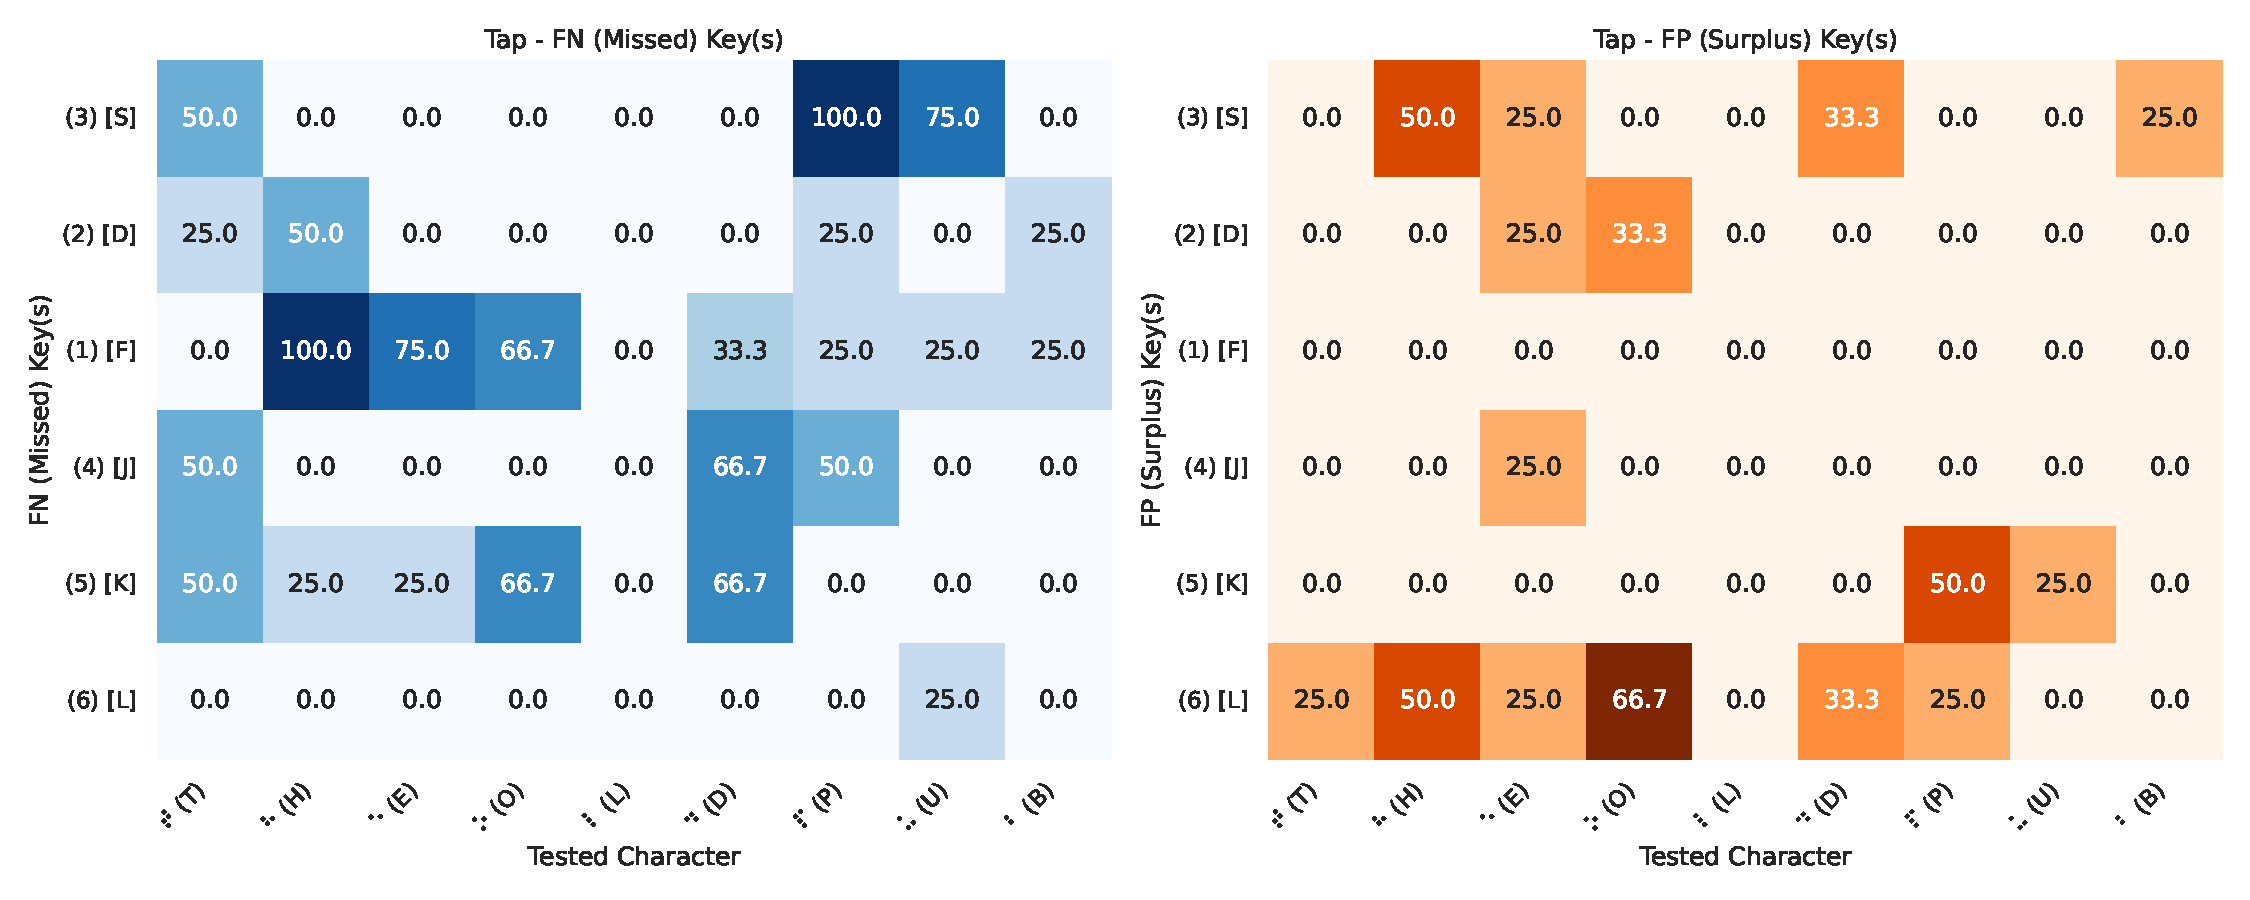
\includegraphics[width=\textwidth]{src/pictures/Study1Data_Experiment/missed_surplus_test_percentages_study1_T.pdf}
        \caption{Tapping Stimulus}
    \end{subfigure}
    \begin{subfigure}[b]{0.45\textwidth}
        \centering
        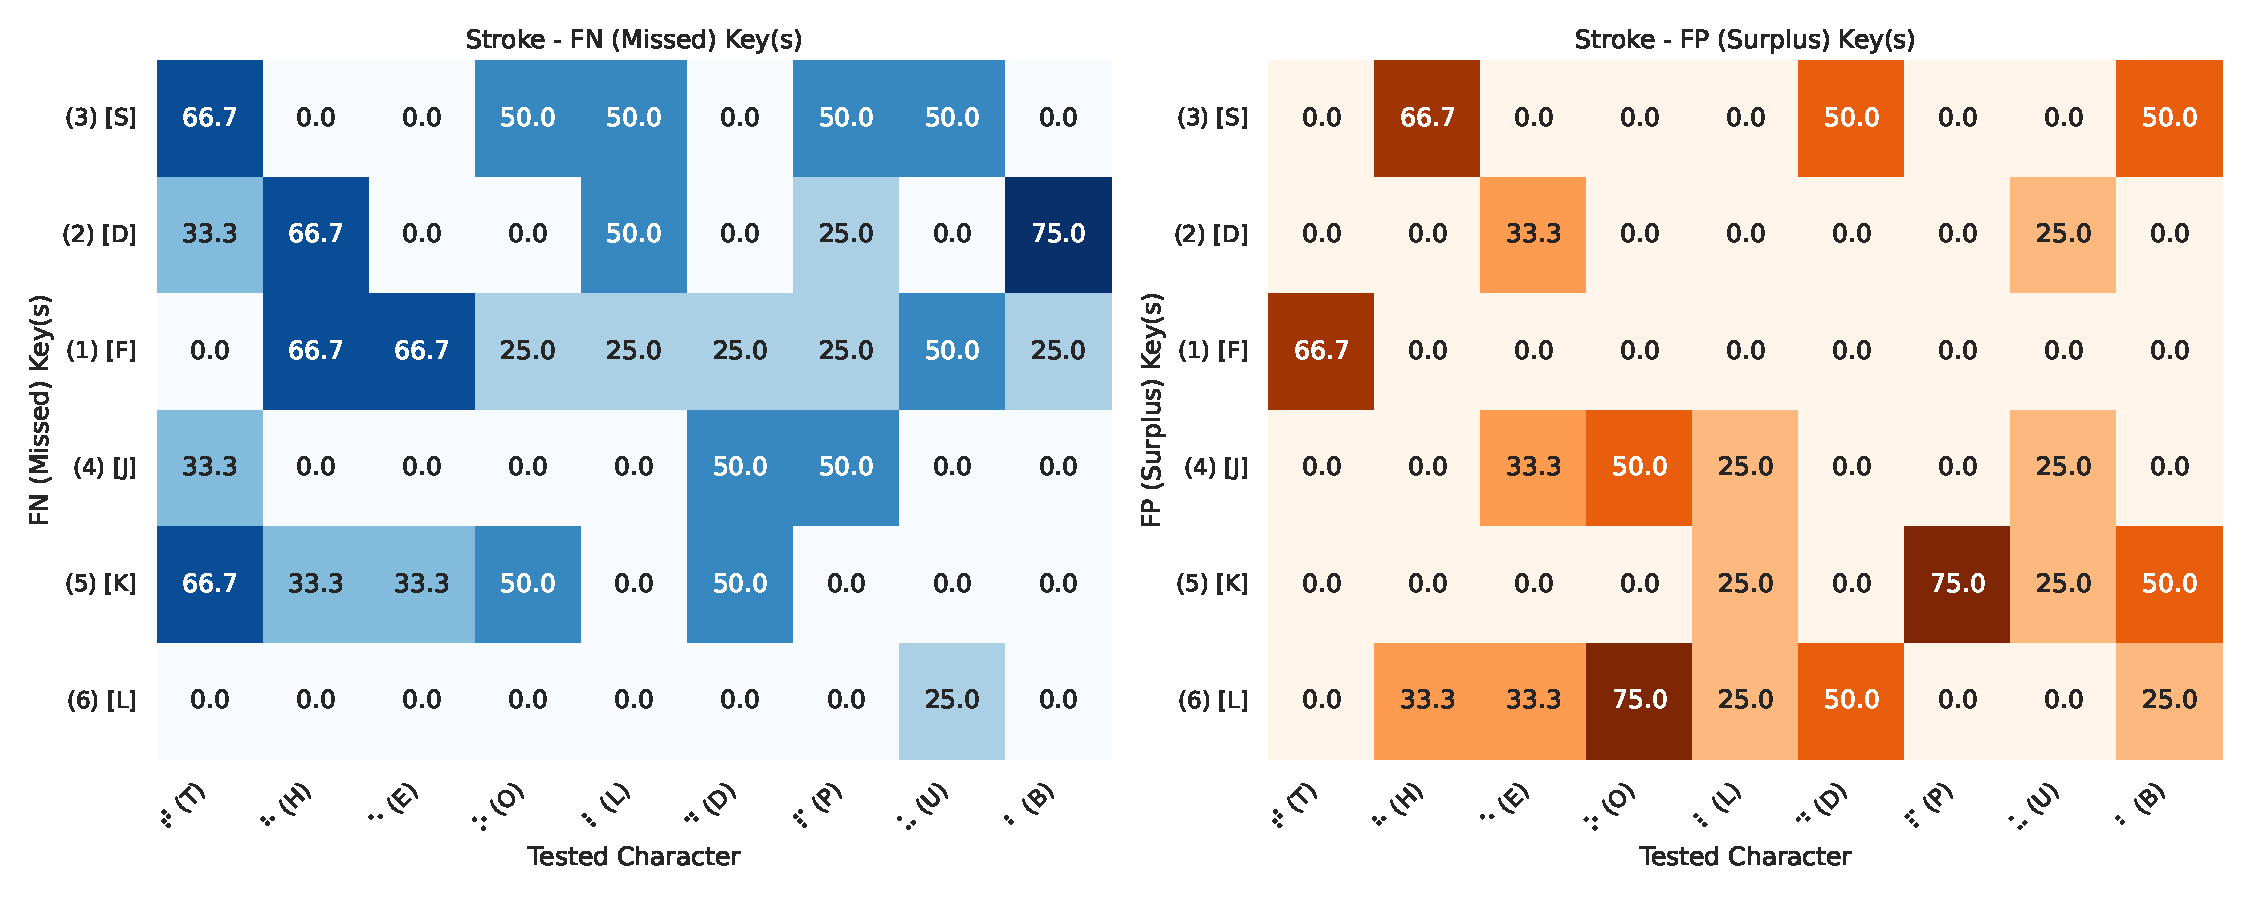
\includegraphics[width=\textwidth]{src/pictures/Study1Data_Experiment/missed_surplus_test_percentages_study1_S.pdf}
        \caption{Stroking Stimulus}
    \end{subfigure}\\
    \begin{subfigure}[b]{0.45\textwidth}
        \centering
        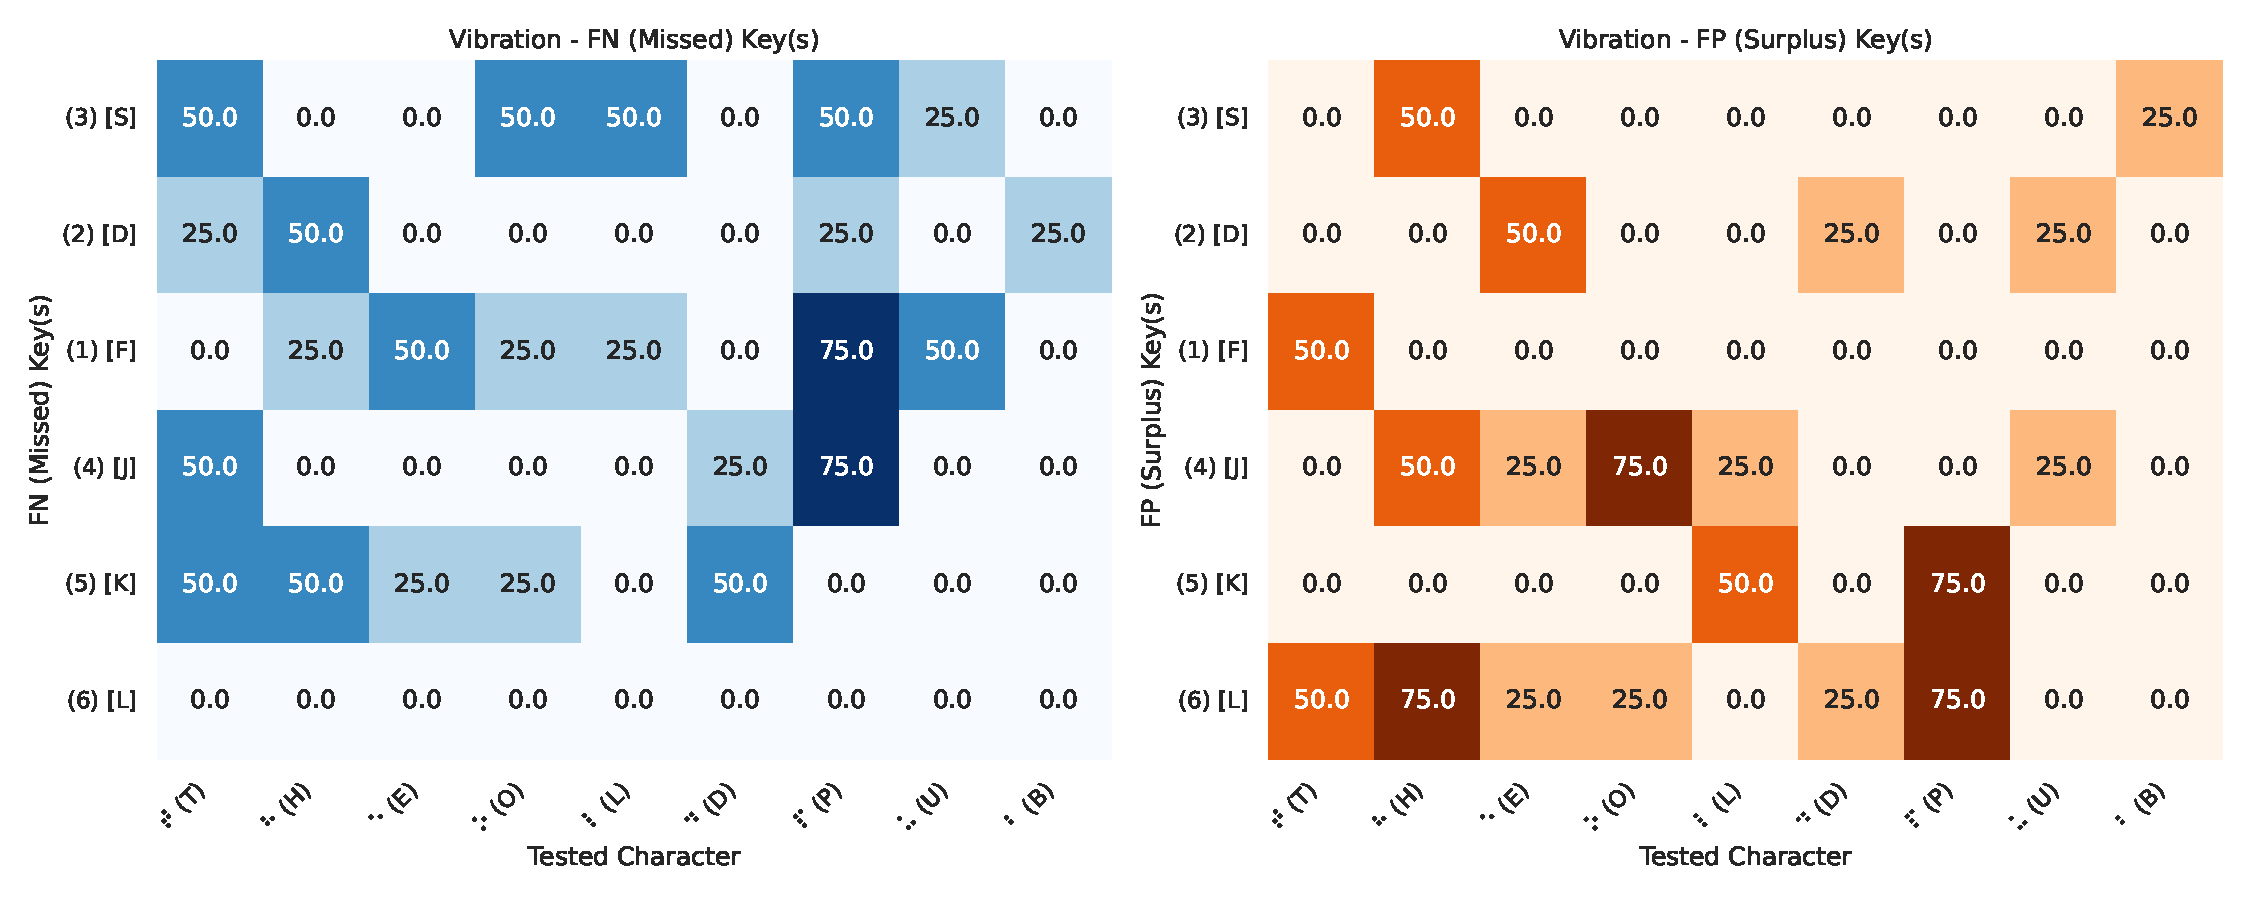
\includegraphics[width=\textwidth]{src/pictures/Study1Data_Experiment/missed_surplus_test_percentages_study1_V.pdf}
        \caption{Vibration Stimulus}
    \end{subfigure}
    \caption{FN (Missed) Character in blue and FP (Surplus) keys in red in percent for each Braille character grouped by stimulus.}
    \label{fig:missed_surplus_percentages_study1}
\end{figure}

After analysing the missed and surplus characters, we now dive deeper into the specific relationships between each tested character and the corresponding surplus or missed character. These details are depicted in \autoref{fig:missed_surplus_percentages_study1}.

The diagram shows each Braille character under the category \enquote{tested character}, with the corresponding pressed keyboard characters on the left. 
The blue sections represent the percentage of missed keys when typing a character, while the red sections indicate surplus pressed keys for each character.

It is important to note that both \autoref{fig:missed_surplus_percentages_study1} and \autoref{fig:missedSurplus_study1} are related. Each column in \autoref{fig:missedSurplus_study1} corresponds to one row of missed or surplus characters in the same stimulus image, with matching colours for the same character. 
Thus, \autoref{fig:missed_surplus_percentages_study1} provides a more detailed, lower-level abstraction of the data shown in \autoref{fig:missedSurplus_study1}.

For the surplus (red) side, significant differences are observed for the Braille characters \braille{b}(B) and \braille{u}(U). For \braille{b}(B), the key \textcircled{3} [S] was consistently pressed incorrectly across all stimuli. However, for the Stroking stimulus, the keys \textcircled{5} [K] and \textcircled{5} [L] were also pressed incorrectly, with percentages of 50\% and 25\%, respectively.

Another notable difference occurs for the Braille character \braille{u}(U), where the key \textcircled{4} [K] was pressed incorrectly for the Tap and Stroking stimuli, and the keys \textcircled{4} [J] and \textcircled{2} [D] were pressed incorrectly for the Stroking and Vibration stimuli.

For the missed characters (FN, in blue), several differences are evident for the Braille characters \braille{l}(L) and \braille{b}(B). There were no missed characters for the Tapping stimulus, but for the Stroking and Vibration stimuli, the keys \textcircled{3} [S] and \textcircled{1} [F] were frequently missed. In the case of Stroking, the key \textcircled{2} [D] was missed in about 50\% of the trials.

A larger difference is seen with the key \textcircled{6} [L], which was never missed for the Vibration stimulus but was missed in about 25\% of cases for both the Stroking and Tapping stimuli.

\begin{figure}
    \centering
    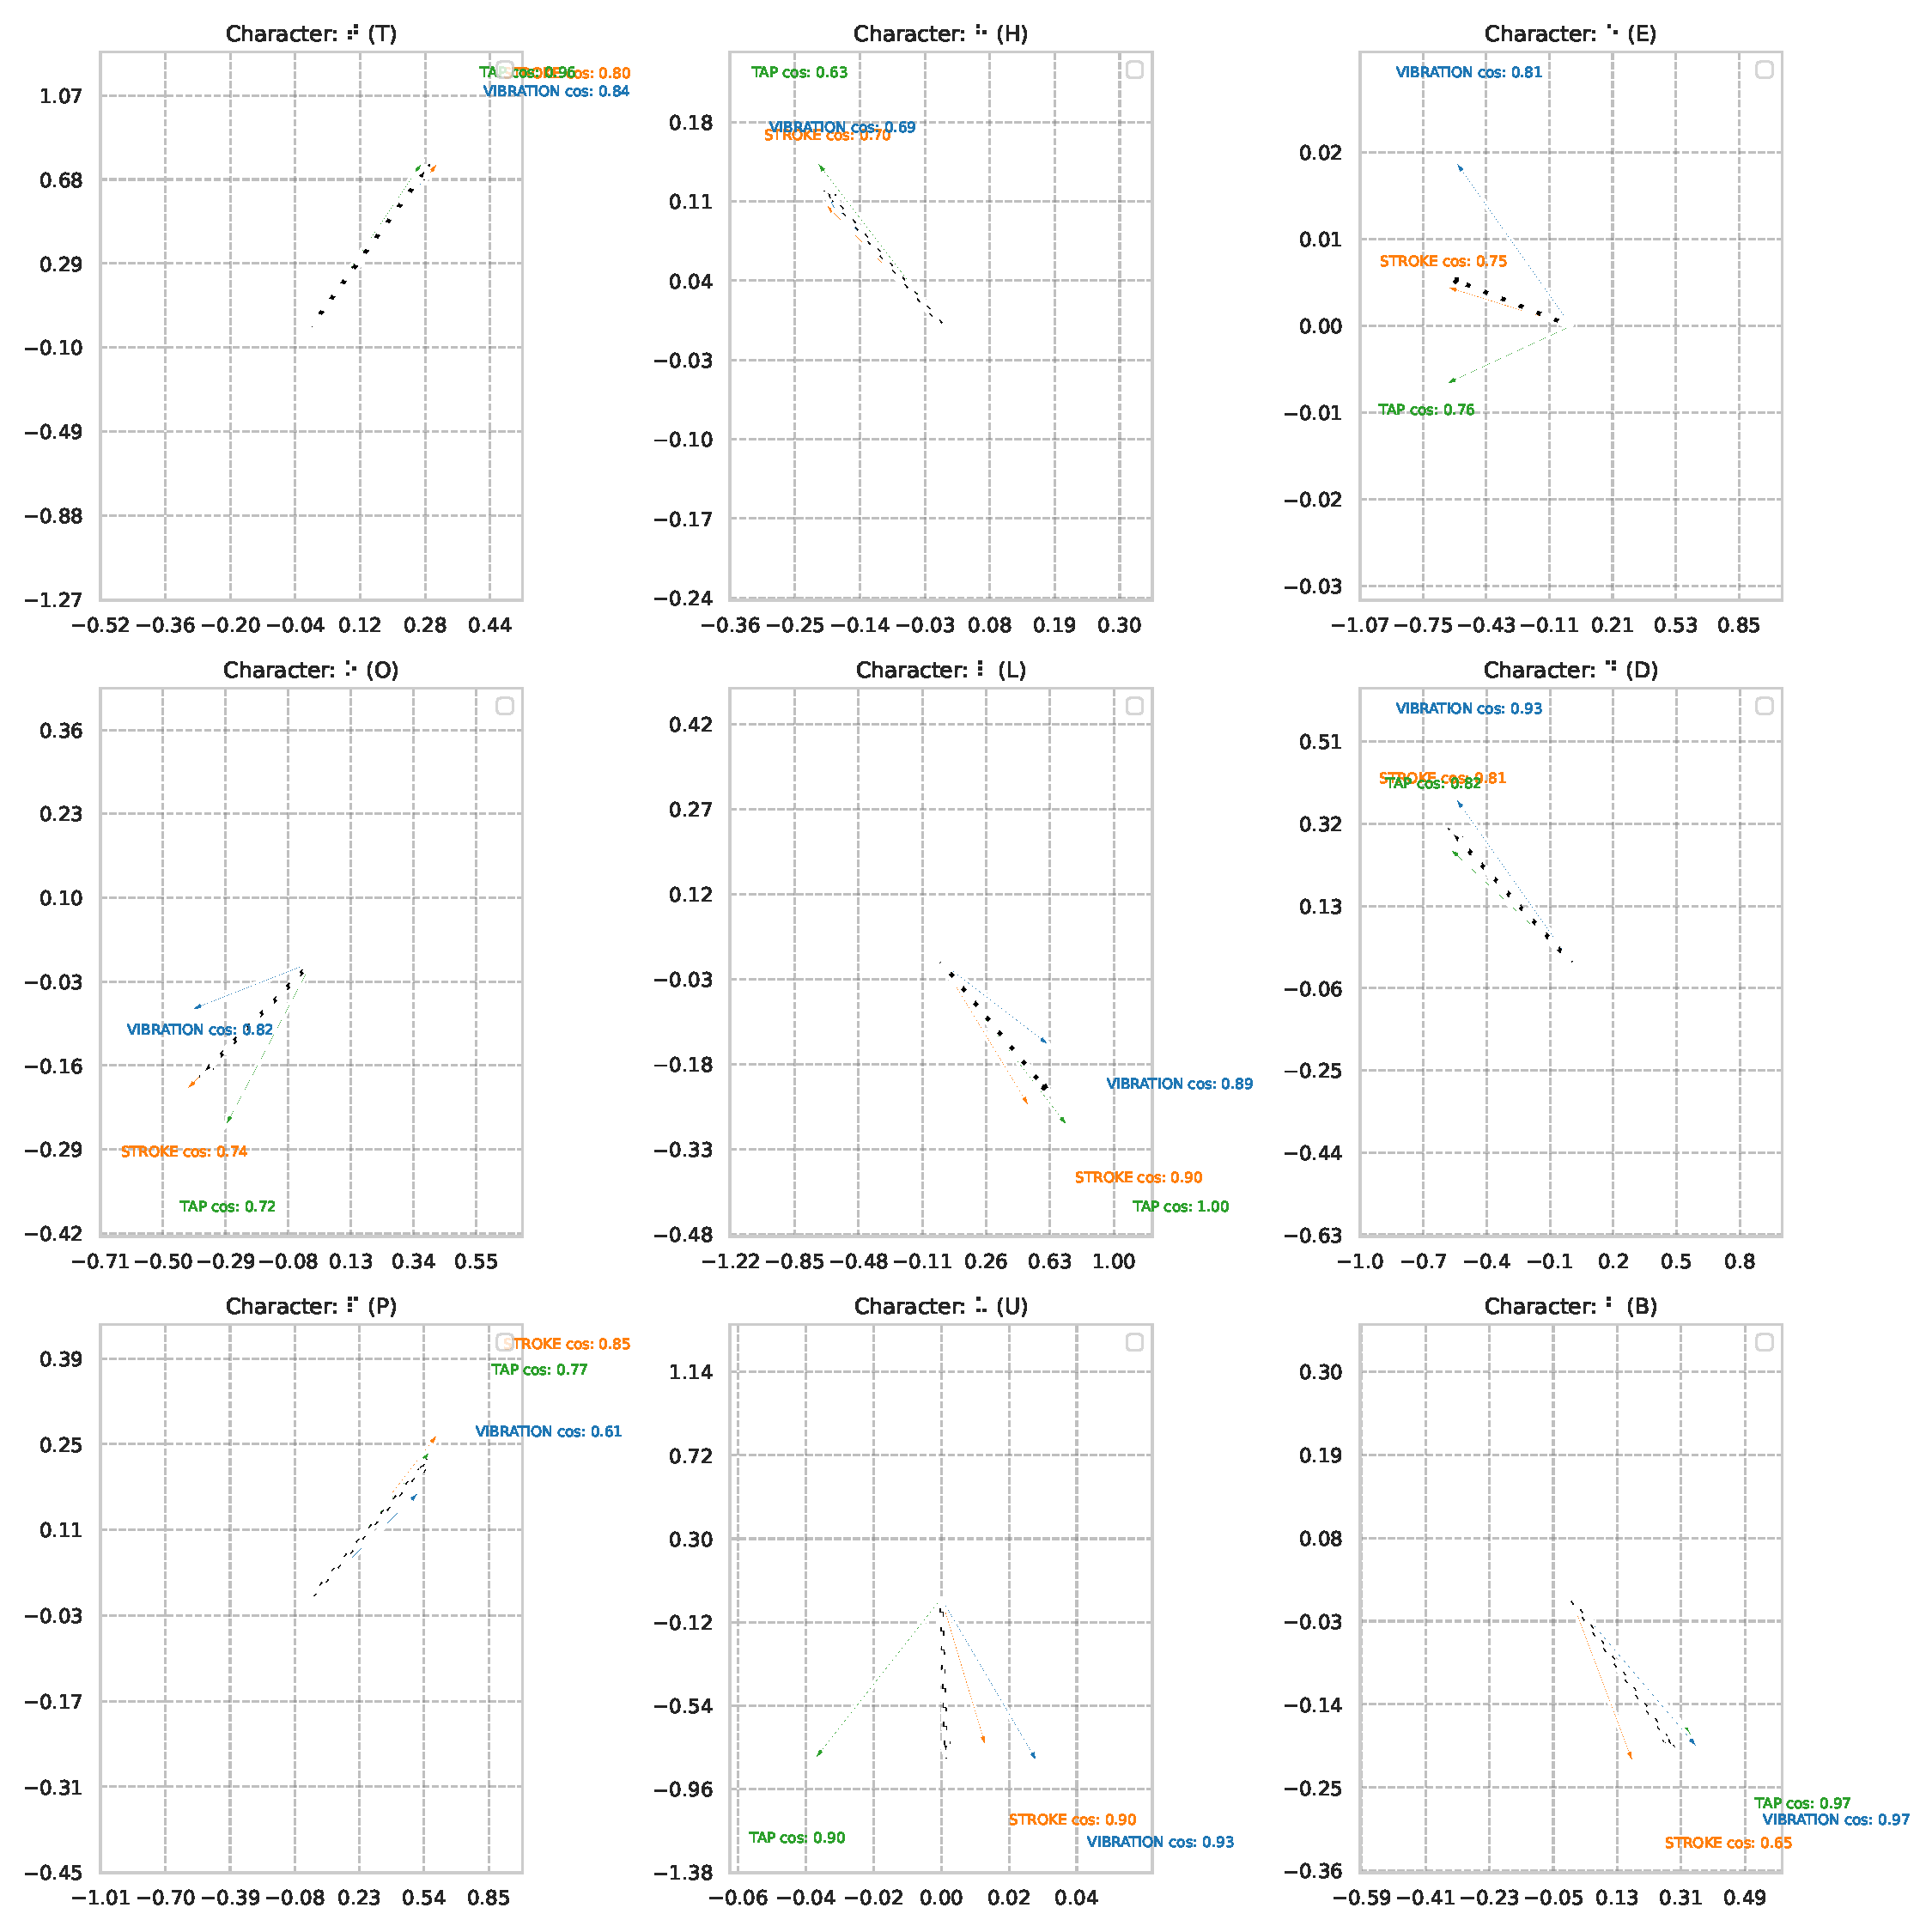
\includegraphics[width=\linewidth]{src/pictures/Study1Data_Experiment/Vectors_study1.pdf}
    \caption{Cosine Similariy for each of the Stimuli.\\Plotted using a \gls{pca} dimensionality reduction.}
    \label{fig:cosSim_PCA_study1}
\end{figure}

Lastly, a one-hot encoding vector was created for the pressed keys for each stimulus, similar to a column in \autoref{fig:missed_surplus_percentages_study1}. 
In order to visually represent the differences between the errors.
We then calculated the cosine similarity for each stimulus character vector embedding against the ground truth, which is depicted by the black dotted line in \autoref{fig:cosSim_PCA_study1}.
To present the cosine similarity in a visually appealing manner, we used \gls{pca} to reduce the dimensionality to two dimensions for plotting.

The cosine similarity and \gls{pca} analysis, as shown in the figure, indicate that despite noise reduction through \gls{pca}, the vectors align in a similar direction. The most noticeable differences were observed for the braille characters \braille{u}(U), \braille{e}(E), and \braille{o}(O).
But their Cosine similarity scores were still very similar with cosine scores of 0.81 (Vibration), 0.76 (Tapping) and 75 (Stroking) for the braille character \braille{e}(E), cosine scores of 0.82 (Vibration), 0.72 (Tapping) and 0.74 (Stroking) for the \braille{o}(O).
And lastly 0.9 (Tapping), 0.93 (Vibration) and 0.9 (Stroking) for the braille character \braille{u}(U)



\subsection{Second Study}

\begin{table}
\resizebox{\columnwidth}{!}{
    \centering
    \begin{tabular}{|c|c|c|c|} \hline 
        Gender & Age & Dominant Hand & Previous Braille Knowledge\\ \hline 
        F & 21 & R & No\\ \hline 
        M & 61 & L & No\\ \hline 
        M & 23 & R & No\\ \hline 
        F & 27 & R & No\\ \hline 
        F & 29 & R & No\\ \hline 
        M & 23 & R & No\\ \hline 
        M & 26 & R & No\\ \hline 
        M & 23 & R & No\\ \hline
    \end{tabular}}
    \caption{Second study participant data}
    \label{tab:study2_participant_data}
\end{table}
\begin{figure}
    \centering
    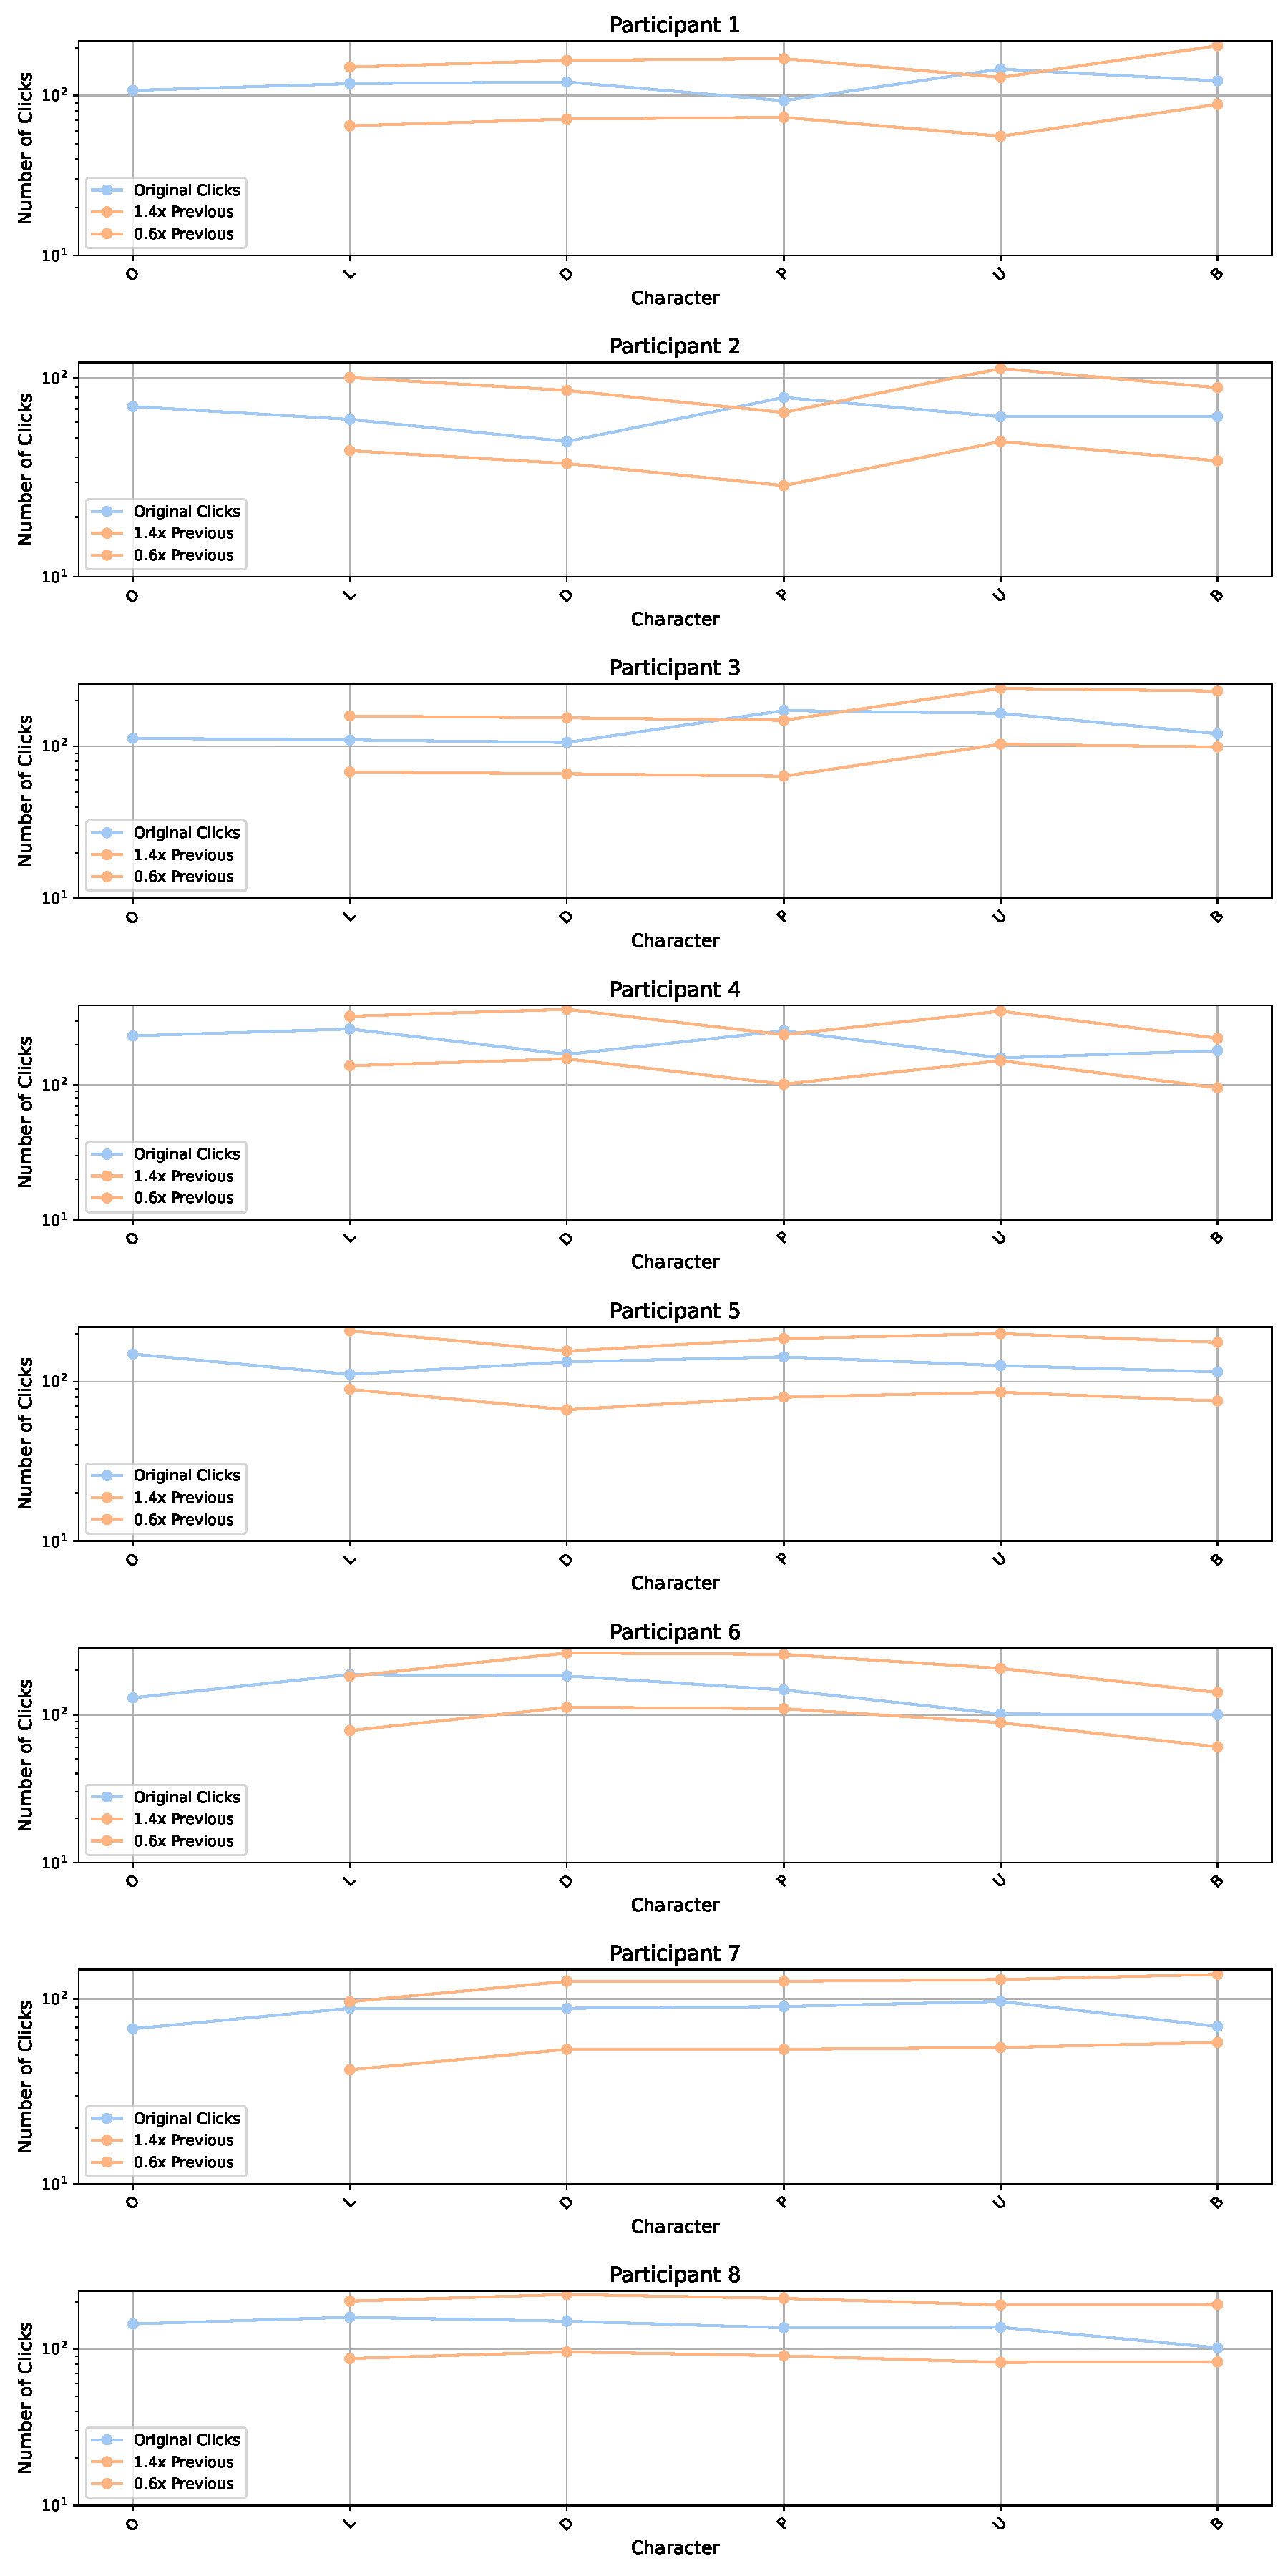
\includegraphics[width=0.5\linewidth]{src/pictures/Study2Data_questionnaire/participantPlots_study2.pdf}
    \caption{Participant Click-differences.}
    \label{fig:participant_clicks-secondStudy}
\end{figure}

For the second study, we interviewed 8 participants (5 male, 3 female) aged between 4 and 61 years, with an average age of 29.125 years and a median age of 24.5 years. Of these, 7 participants were right-handed and 1 was left-handed, as shown in \autoref{tab:study2_participant_data}. None of the participants had prior knowledge of Braille.


\begin{figure}
    \centering
    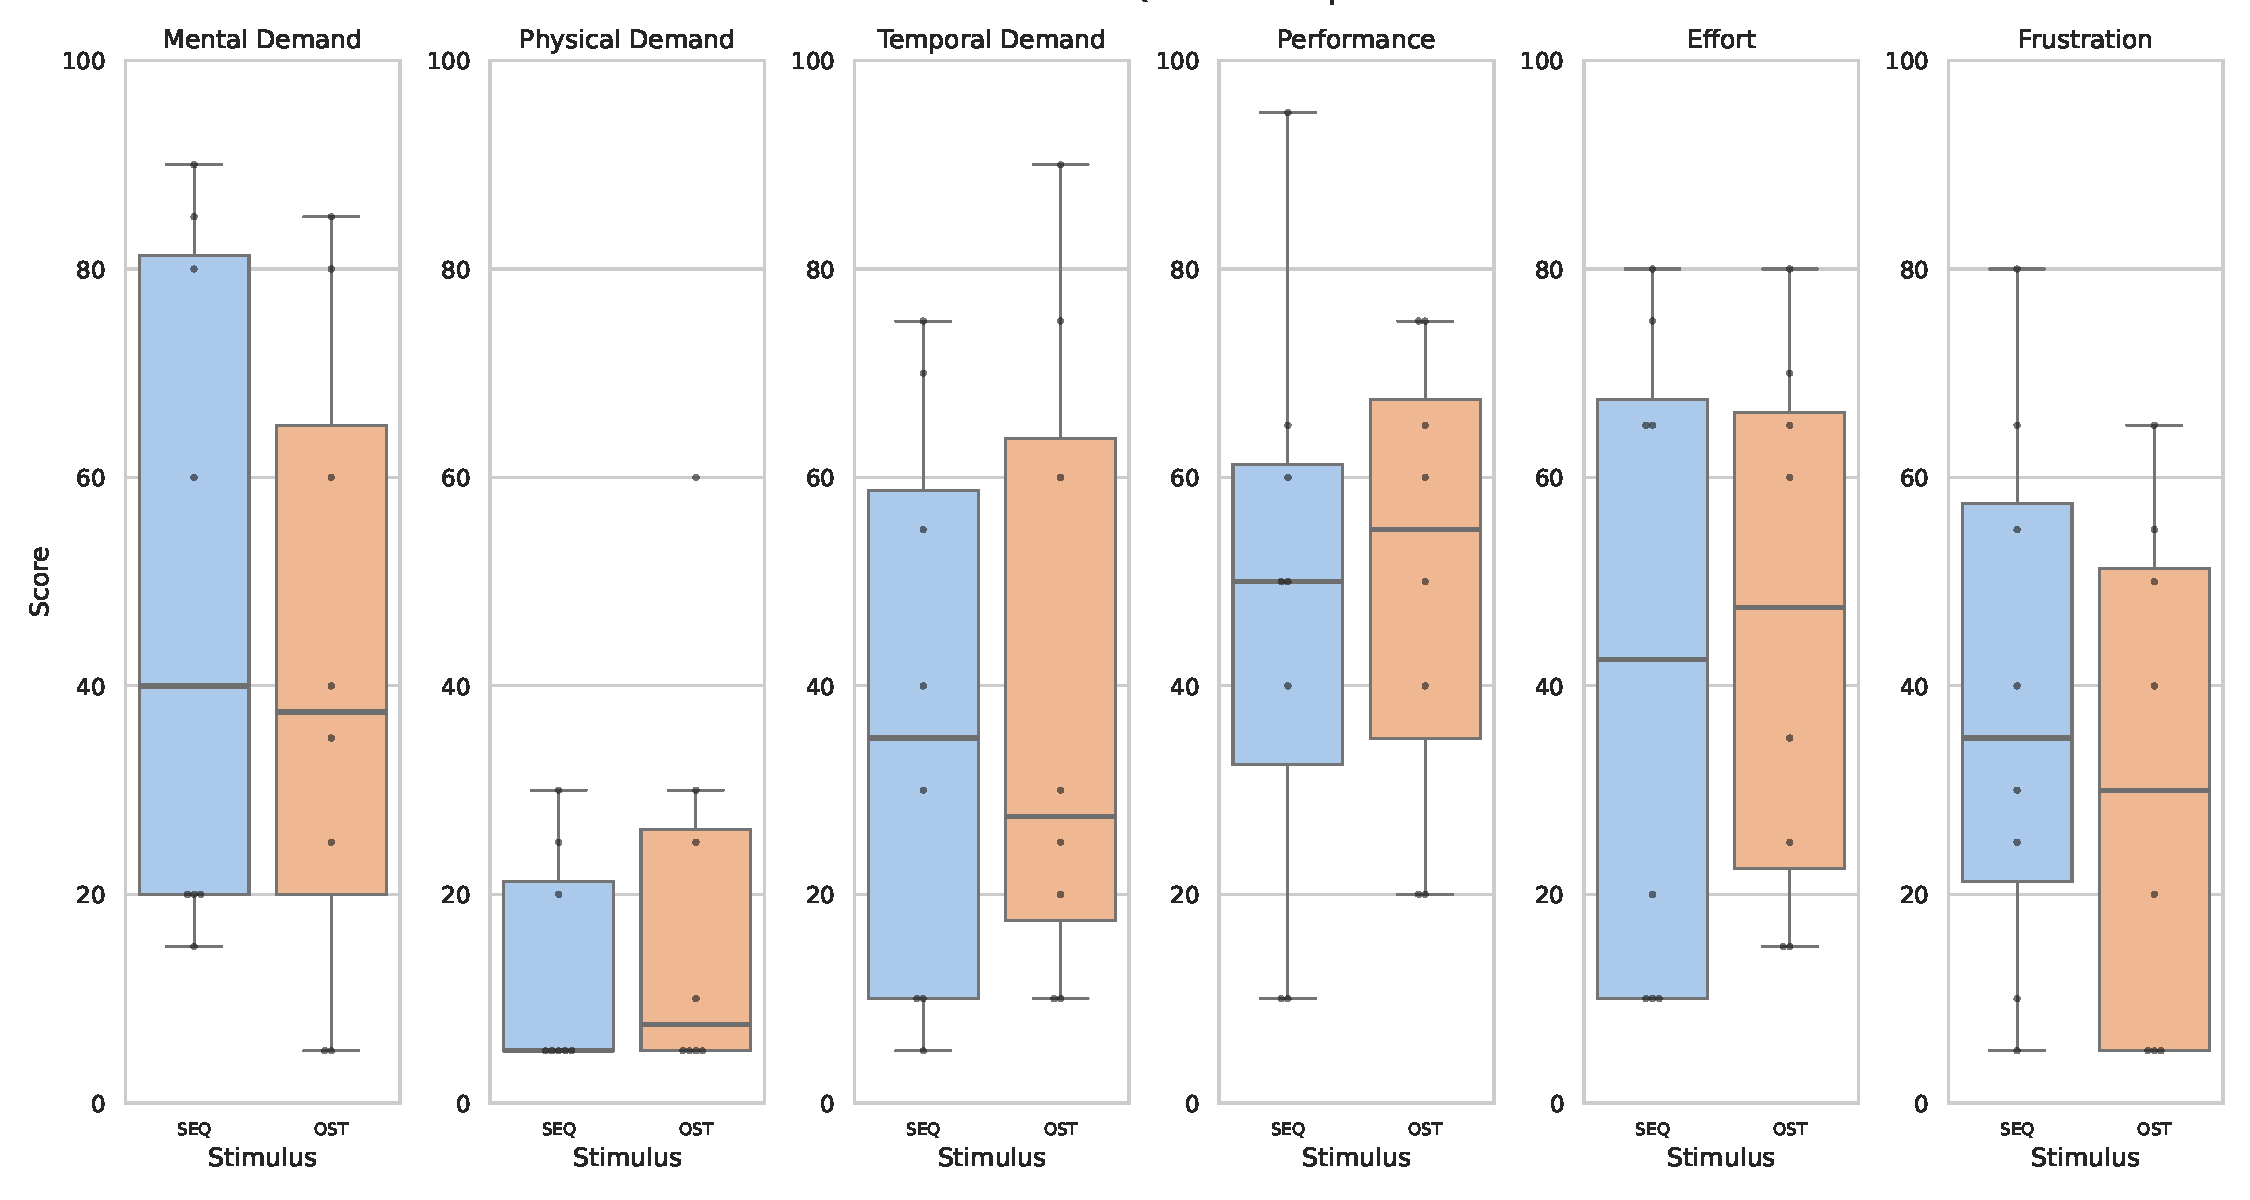
\includegraphics[width=\linewidth]{src/pictures/Study2Data_questionnaire/nasaTLX_study2.pdf}
    \caption{Raw Nasa TLX scores of the different Encodings grouped by the Nasa TLX dimensions.}
    \label{fig:nasaTLX-secondStudy}
\end{figure}

Consistent with the first study, we conducted a NASA TLX test after each encoding sequence to assess the task load experienced by the participants. The results of the NASA TLX are presented in \autoref{fig:nasaTLX-secondStudy}, where each encoding is displayed as a box plot grouped by the NASA TLX dimensions.

As shown, the respective box plots for the dimensions appear similar, with medians of $40$ for \gls{seq} and $35$ for \enquote{ost} under the \enquote{Mental Demand} category. The Q1-Q3 quantiles for \gls{seq} range from $20$ to $82$, while for \enquote{ost}, they range from $20$ to $65$.

For the \enquote{Physical Demand} category, the median for \gls{ost} is slightly lower at $5$, compared to the median of approximately $7.5$ for \gls{seq}. The Q1-Q3 quantiles start at $5$ for both encodings, but \gls{seq} extends up to $22.5$, while \enquote{ost} reaches $25$.

In the \enquote{Temporal Demand} category, the medians are $35$ for \gls{seq} and $30$ for \enquote{ost}, with similar quantile ranges—$10$ to $57.5$ for \gls{seq} and $17.5$ to $65$ for \enquote{ost}.

Similar to the previous categories, the median for \gls{seq} in the \enquote{Frustration} category is higher, at $35$, compared to the median of $30$ for \enquote{ost}.

For the \enquote{Performance} and \enquote{Effort} categories, the medians show a similar trend. The median for \gls{seq} is $50$ in the \enquote{Performance} category, while \enquote{ost} has a median of $55$. For \enquote{Effort}, the median for \gls{seq} is $42.5$, whereas \enquote{ost} has a median of $47.5$.

To assess the significance of the NASA TLX results, we conducted \gls{mwu} significance tests, with the outcomes presented in \autoref{table:nasaTLX_significance_secondStudy_nonParam}. As shown, all p-values are relatively high, indicating that the null hypothesis ($H_0$) was not rejected.

\begin{table}[ht]
\resizebox{\columnwidth}{!}{
\centering
\begin{tabular}{|l|l|l|l|l|}
\hline
\textbf{Question} & \textbf{Test Statistic} & \textbf{p-value}  &\textbf{Significance}           &\textbf{Effect Size}\\ \hline
\textbf{Mental Demand}        & 35.500& 0.7513&Not Significant &0.2141\\ \hline
\textbf{Physical Demand}      & 27.000& 0.6019&Not Significant &0.3559\\ \hline
\textbf{Temporal Demand}      & 29.0000& 0.7911&Not Significant &0.1065\\ \hline
 \textbf{Performance}          & 27.5000& 0.6721&Not Significant &0.1228\\\hline
 \textbf{Effort}               &  27.500& 0.672&Not Significant &0.1285\\\hline
 \textbf{Frustration}          & 39.0000& 0.4907&Not Significant &0.3168\\\hline
\end{tabular}}
\caption{Results of \gls{mwu} significance tests for the different NasaTLX dimensions with Cohens d.}
\label{table:nasaTLX_significance_secondStudy_nonParam}
\end{table}

\begin{figure}
    \centering
    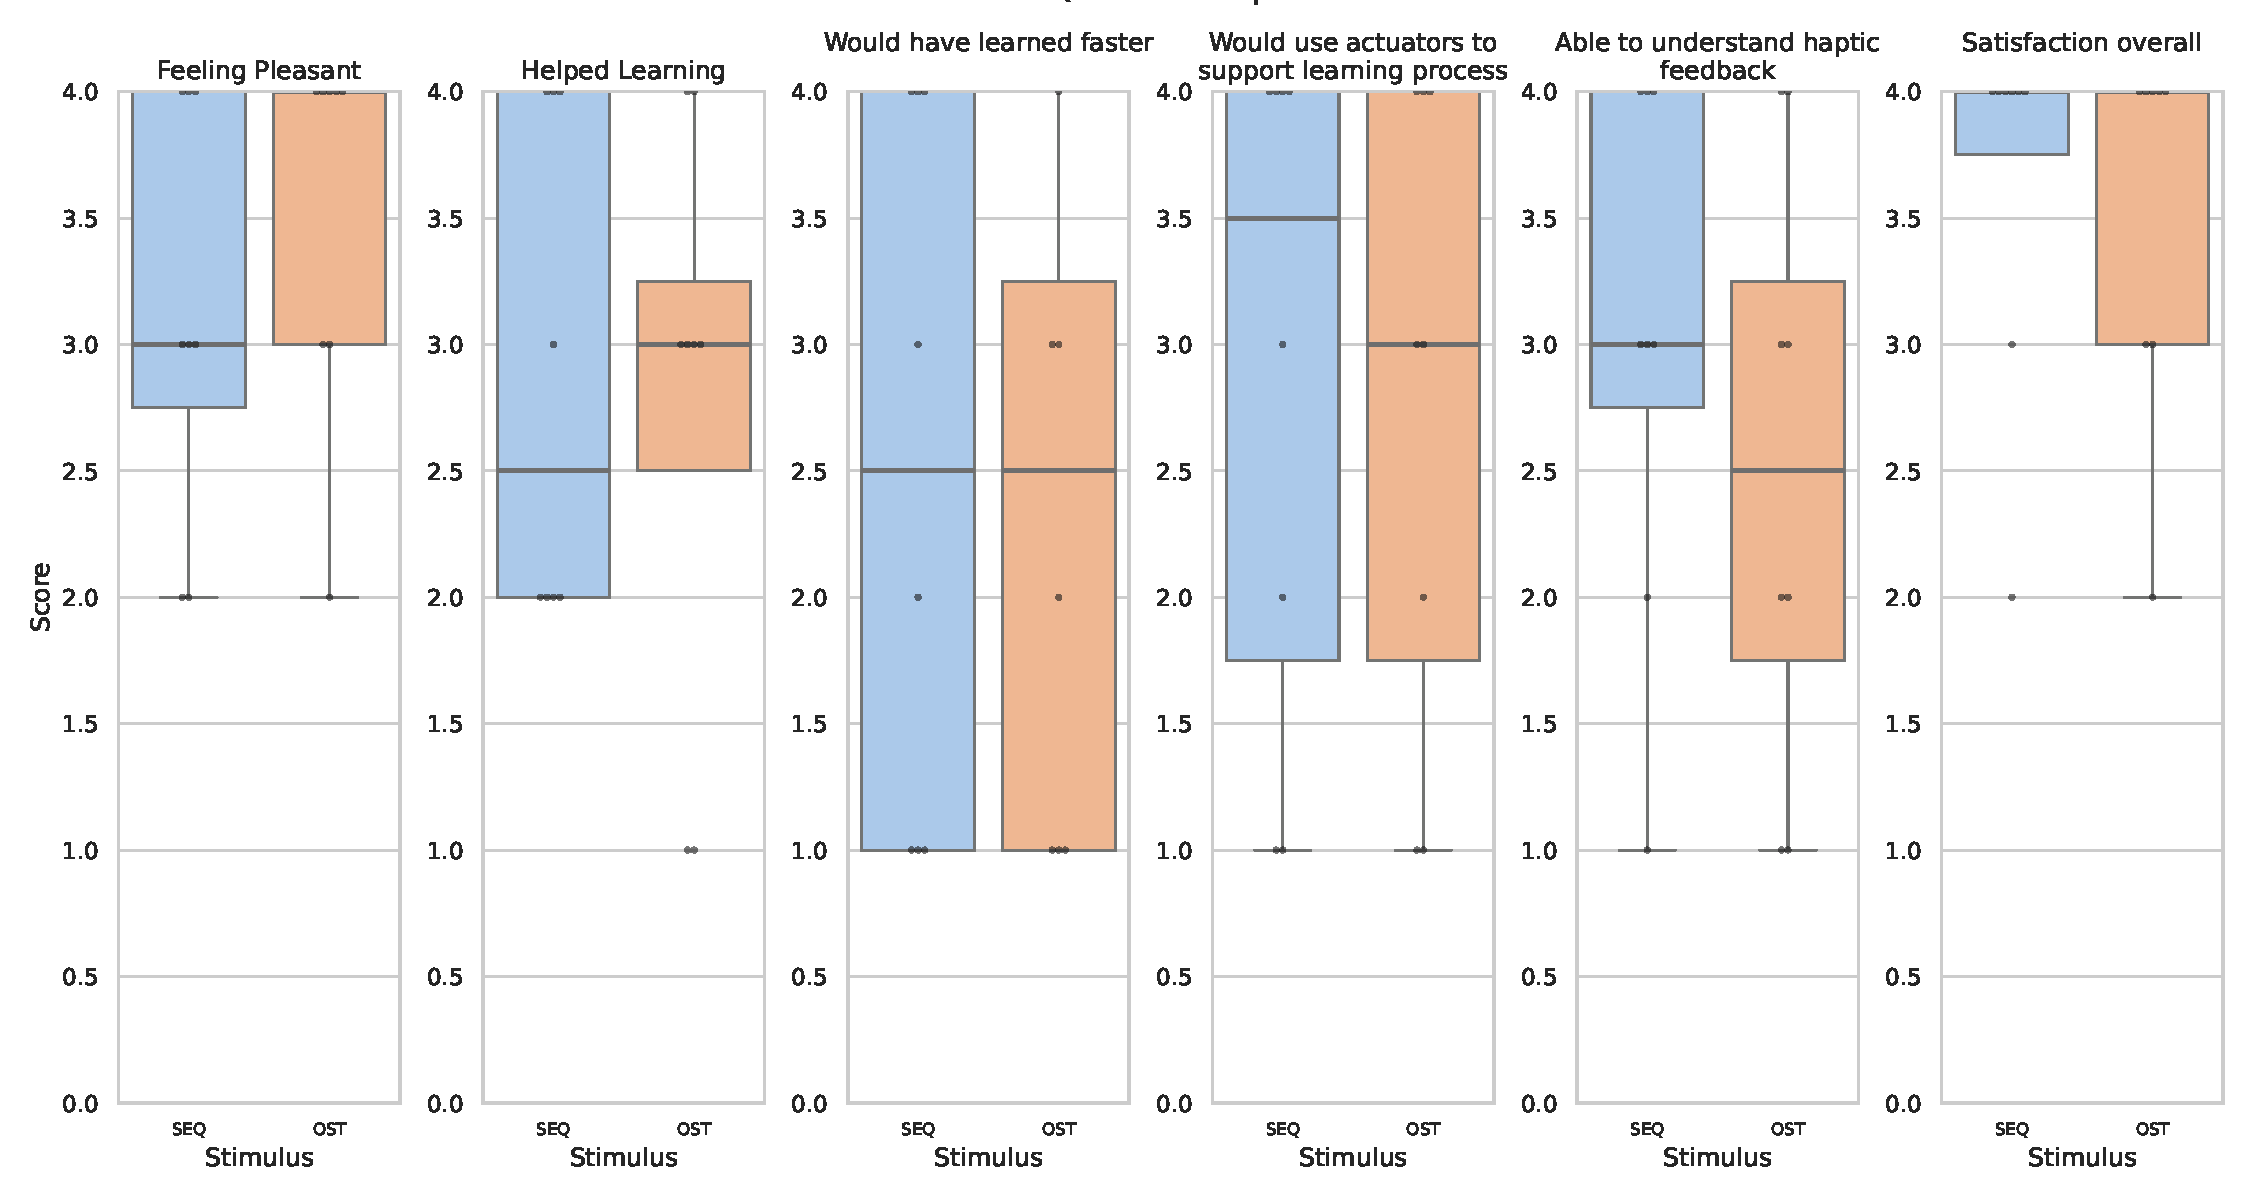
\includegraphics[width=\linewidth]{src/pictures/Study2Data_questionnaire/questions_special_study2.pdf}
    \caption{Self-assessment Results of the different Stimuli grouped by the self-assessment categories.}
    \label{fig:questions_individual_secondStudy}
\end{figure}

Following the NASA TLX task load, participants were asked to evaluate their experiences with the two different encodings. Their evaluations were plotted across six different dimensions, as shown in \autoref{fig:questions_individual_secondStudy}.

The largest differences in medians were observed in the categories: \enquote{Helped Learning}, with medians of $2.5$ for \gls{seq} and $3$ for \gls{ost}; \enquote{Would use actuators to support the learning process}, with $3.5$ for \gls{seq} and $3$ for \gls{ost}; \enquote{Able to understand haptic feedback}, with $3$ for \gls{seq} and $2.5$ for \gls{ost}; and \enquote{Satisfaction overall}, with $3.75$ for \gls{seq} and $3$ for \gls{ost}. 

The medians for the categories \enquote{Feeling Pleasant} ($3$) and \enquote{Would have learned faster} ($2.5$) were the same for both encodings. 

The Q1-Q3 quantile ranges differed notably in the \enquote{Helped Learning} category, where \gls{seq} ranged from $2$-$4$ and \gls{ost} from $2.5$-$3.25$. In \enquote{Satisfaction overall}, the difference was also noticeable, with \gls{seq} ranging from $3.75$-$4$ and \gls{ost} from $3$-$4$. 

For the \enquote{Would have learned faster} category, the quantile ranges showed a significant difference, with \gls{seq} and \gls{ost} both starting at Q1 = $1$, but \gls{seq} extending to $4$ and \gls{ost} to $3$. 

Finally, the quantile ranges for the \enquote{Able to understand haptic feedback} dimension were nearly identical, with \gls{seq} ranging from $2.75$-$4$ and \gls{ost} from $1.75$-$3.25$.

For the self-assessment tests, we also conducted \gls{mwu} significance tests, and the results are presented in \autoref{table:individualQuestions_significance_secondStudy_nonPara}.
The lowest p-value was found for the \enquote{Feeling Pleasant} dimension; however, with a p-value of $0.3596$, it remains too high to indicate statistical significance.
Therefore, there is no significant difference between the two encodings in terms of self-assessment for usability and their effectiveness in aiding learning.

\begin{table}[ht]
\resizebox{\columnwidth}{!}{
\centering
\begin{tabular}{|l|l|l|l|l|}
\hline
\textbf{Question} & \textbf{U-statistic}& \textbf{p-value}  &\textbf{Significance}           &\textbf{Effect Size}\\ \hline
\textbf{Feeling Pleasant}& 23.5000& 0.3596&Not Significant &0.2232\\ \hline
\textbf{Helped Learning}& 33.0000& 0.9565&Not Significant &0.0263\\ \hline
\textbf{Would have learned faster}& 32.5000& 1.000&Not Significant &0.0131\\ \hline
 \textbf{Would use actuators to support learning process}& 34.5000& 0.8244&Not Significant &0.0656\\\hline
 \textbf{Able to understand haptic feedback}&  40.0000& 0.4139&Not Significant &0.2100\\\hline
 \textbf{Satisfaction overall}& 35.5000& 0.7001&Not Significant &0.0919\\\hline
\end{tabular}}
\caption{Results of the \gls{mwu} test for significance grouped by the different self-assessment dimensions with a Cohens d Effect Size.}
\label{table:individualQuestions_significance_secondStudy_nonPara}
\end{table}

\begin{figure}
    \centering
    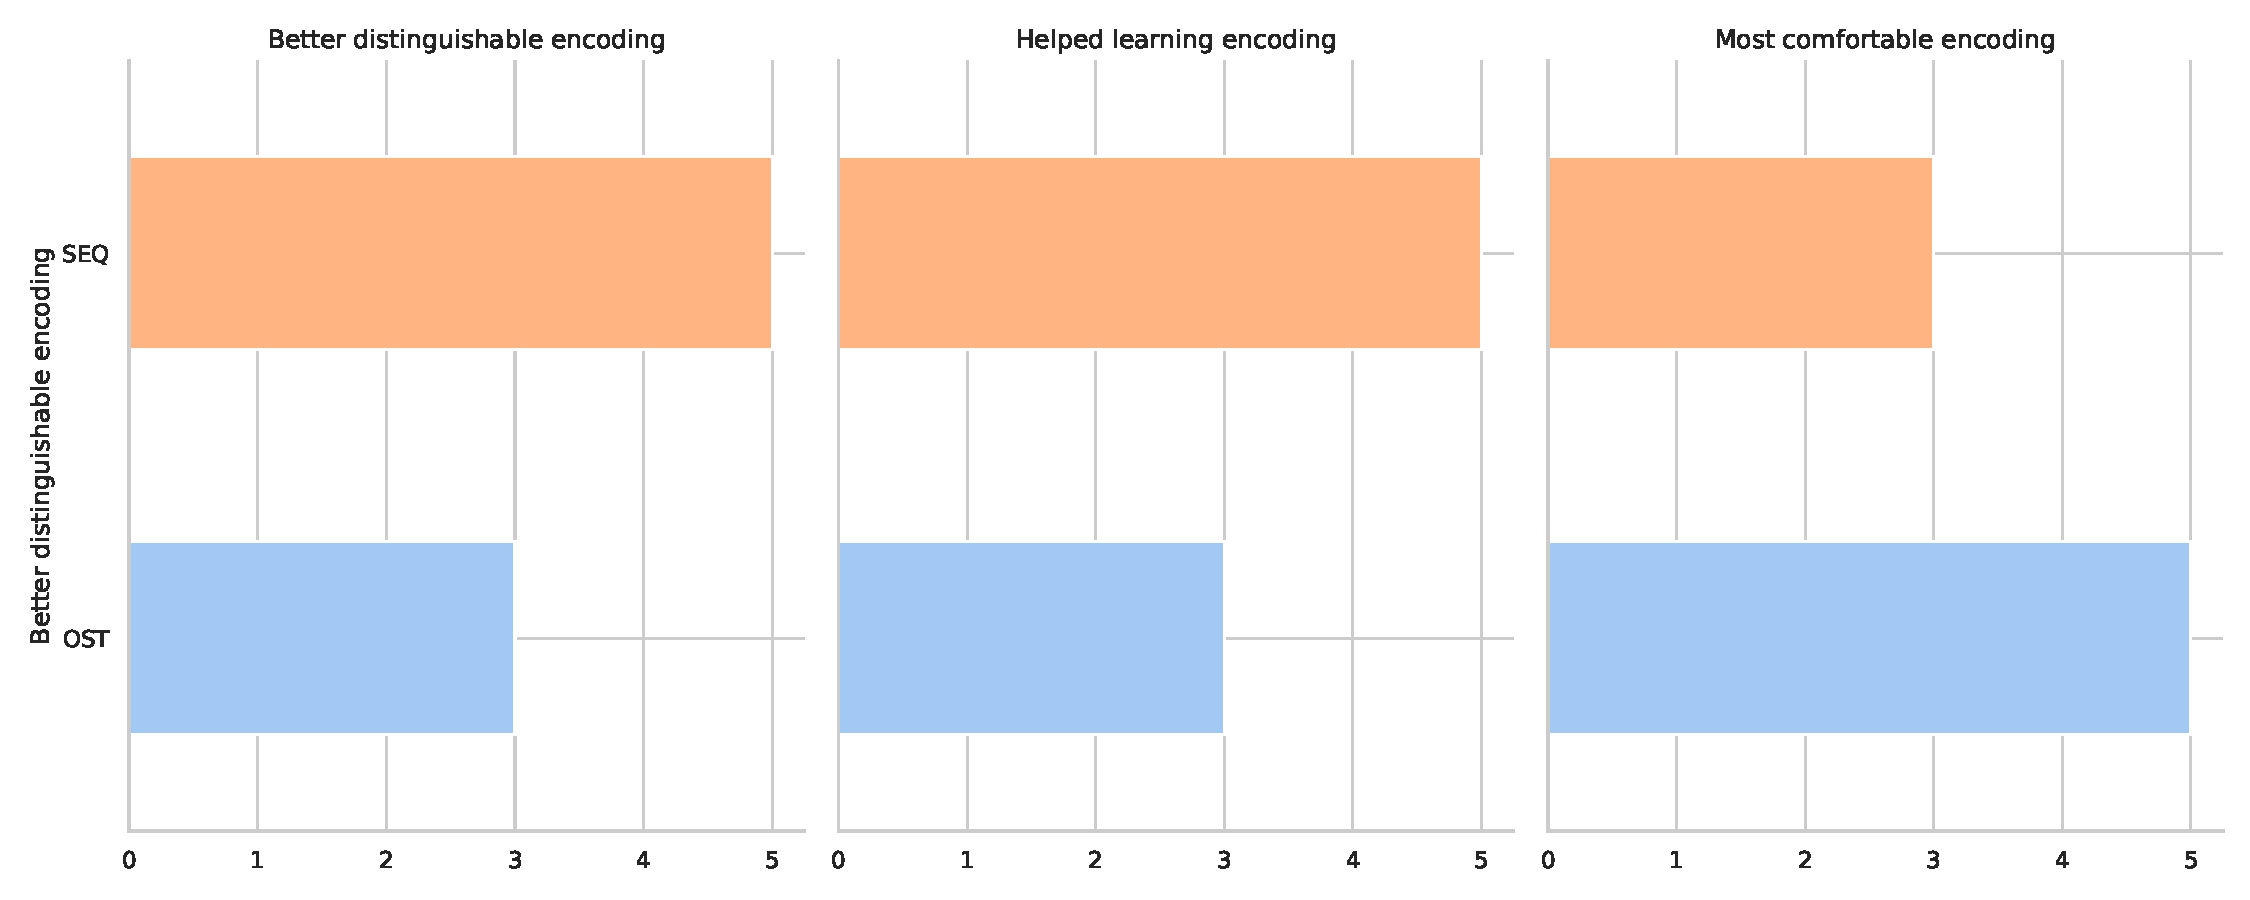
\includegraphics[width=\linewidth]{src/pictures/Study2Data_questionnaire/questions_compare_study2.pdf}
    \caption{Results of the direct comparison between the different encodings.}
    \label{fig:questionsCompare-secondStudy}
\end{figure}

After the study, we asked the participants to compare the two encoding methods, and the results are presented in \autoref{fig:questionsCompare-secondStudy}.
The comparison reveals that the \gls{seq} encoding was perceived as more distinguishable, with $62.5\%$ of participants agreeing, and it was also considered more helpful for learning with the same proportion.
However, the \gls{ost} encoding was regarded as more comfortable, with $62.5\%$ of participants reporting it as more comfortable than the \gls{seq} encoding.

A statistical analysis, presented in \autoref{table:statistical_tests_comparrisson_secondStudy}, showed that conducting the \gls{csgf} study resulted in no significant difference.
The \gls{csgf} was chosen due to insufficient data for a Chi-Squared test.

\begin{table}
\resizebox{\columnwidth}{!}{
    \centering
    \begin{tabular}{|c|c|c|c|}\hline
        Question & \gls{csgf} & p-value & Significance \\\hline
         \enquote{Better distinguishable encoding} & 0.5 & 0.4795& Not Significant\\\hline
         \enquote{Helped Learning encoding} & 0.5 & 0.4795 & Not Significant\\\hline
         \enquote{Most comfortable encoding}& 0.5 & 0.4795 & Not Significant\\\hline
    \end{tabular}}
    \caption{Statistical \gls{csgf} Results for the direct comparison between the stimuli.}
    \label{table:statistical_tests_comparrisson_secondStudy}
\end{table}




\begin{figure}
    \centering
    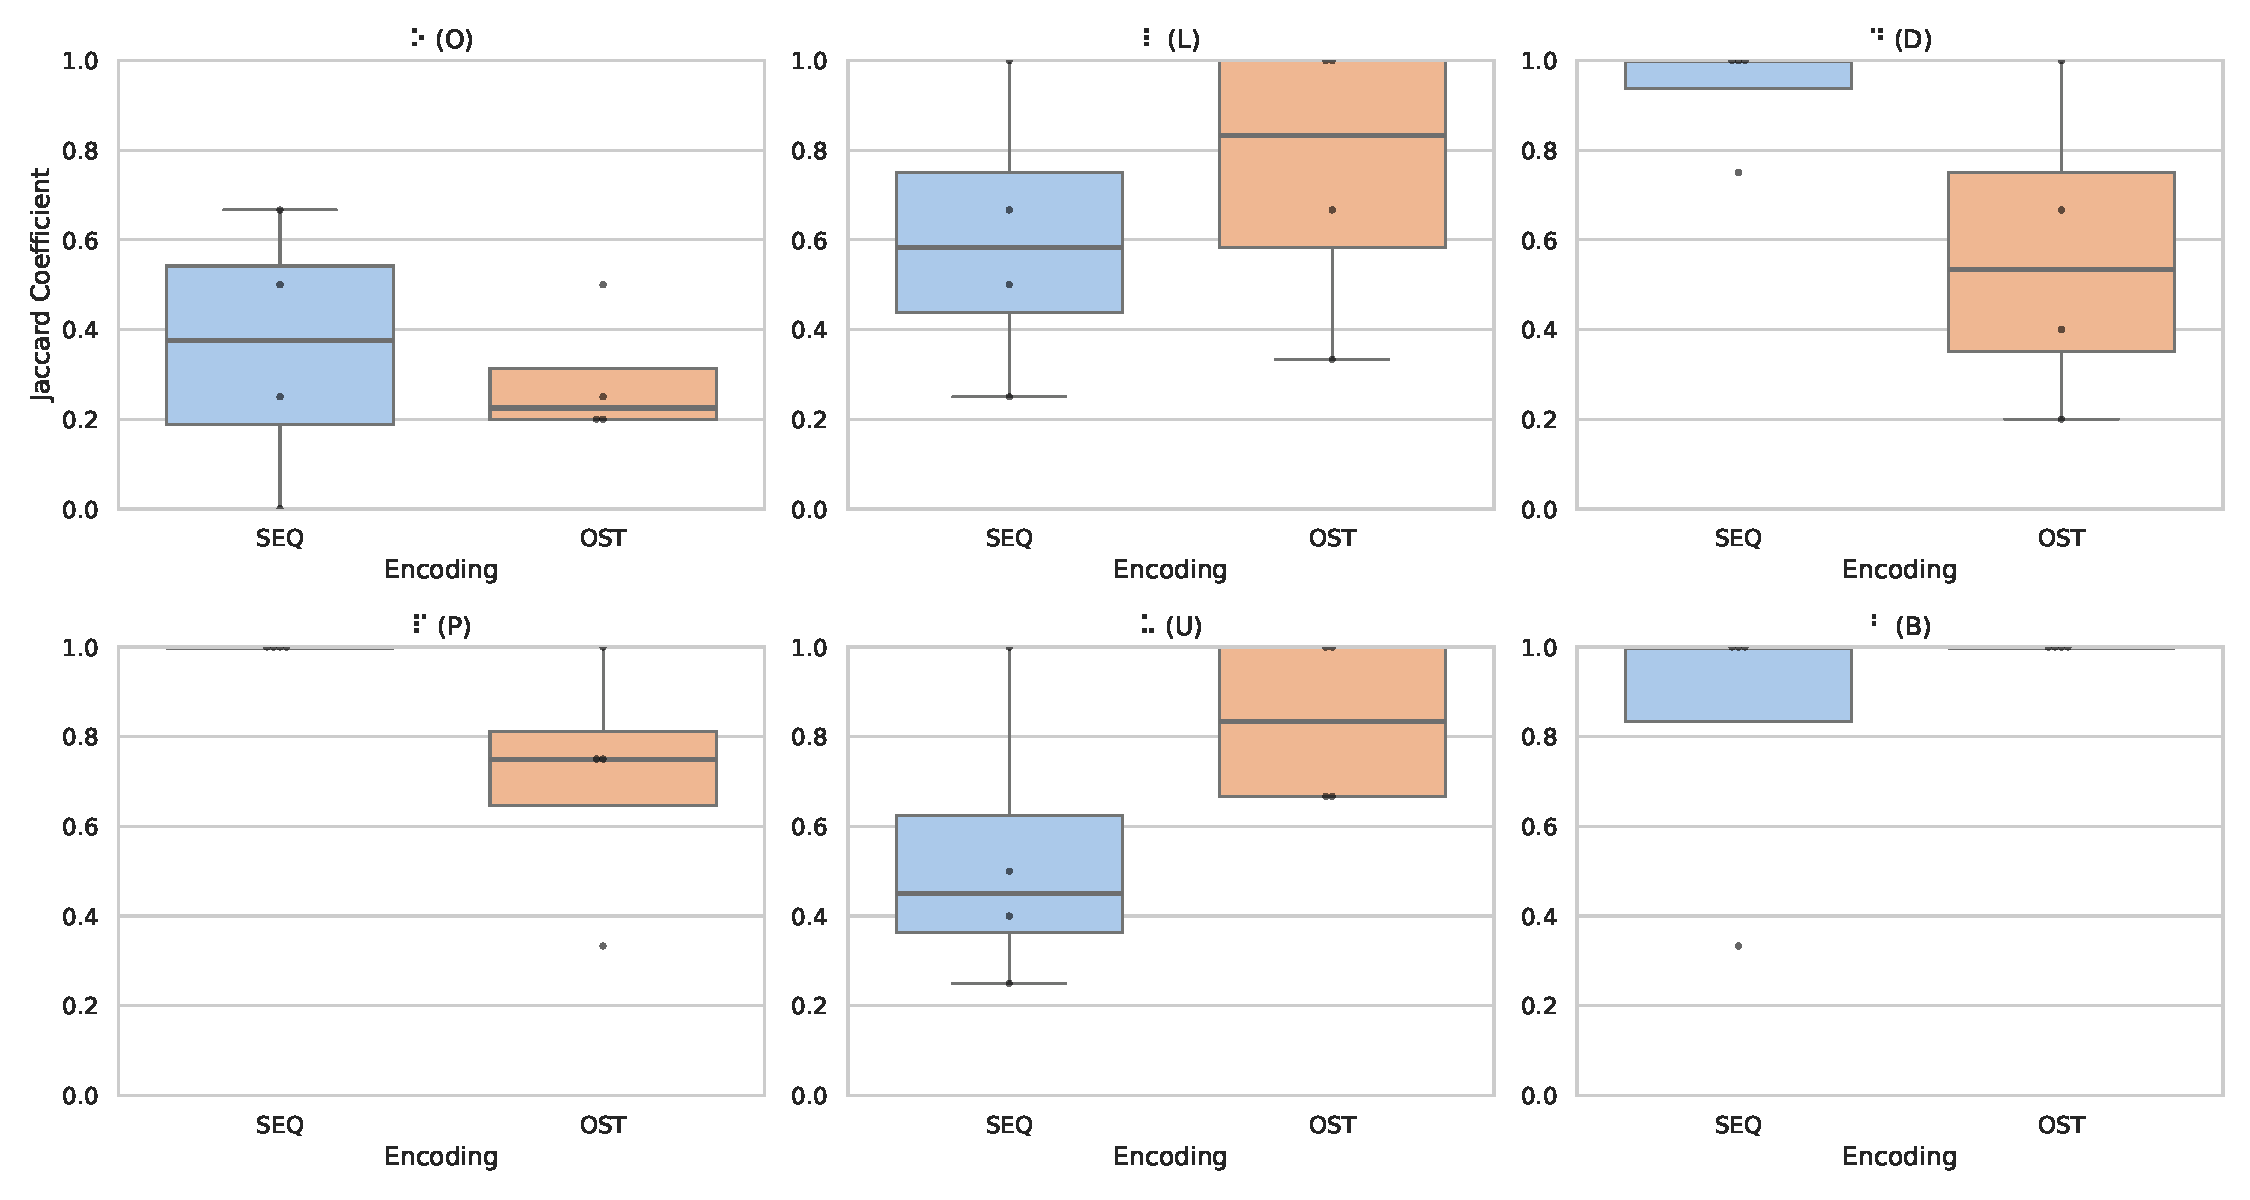
\includegraphics[width=\linewidth]{src/pictures/Study2Data_Experiment/study2_learning_results.pdf}
    \caption{Jaccard coefficient results grouped by the Braille characters during learning for the different Encodings.}
    \label{fig:learning_results_secondStudy}
\end{figure}

During the learning process, we measured performance using the Jaccard and Dice scores. The Jaccard results after learning each character are shown in \autoref{fig:learning_results_secondStudy}, as they are more stringent than the Dice scores.

The charts reveal larger differences in the medians for \braille{d}(D), with a median of $0.95$ for \gls{seq} and $0.55$ for \gls{ost}.
Similarly, for the \braille{u}(U) test, the median difference is substantial, with \gls{seq} showing a median of about $0.45$ and \gls{ost} performing better with a median of $0.825$.
\gls{ost} also outperformed \gls{seq} for the character \braille{l}(L), with a median of $0.825$ compared to $0.575$ for \gls{seq}.
For the character \braille{b}(B), \gls{ost} showed better performance, with a median of $1$, which was consistent across the Q1 and Q3 quantiles. In comparison, \gls{seq} had a median of $0.825$, with Q1 equal to that value and Q3 at $1$.
However, for the character \braille{p}(P), \gls{seq} performed better, with a median, Q1, and Q3 of $1$, compared to \gls{ost}, which had a median of $0.75$, Q1 of $0.65$, and Q3 of $0.82$.

Afterwards, we conducted the appropriate \gls{mwu} tests for significance, and the results are shown in \autoref{table:learning_significance_results_secondStudy}.
However, none of the tests showed statistically significant differences.
The lowest p-value was observed in the \braille{b}(B) test, with a value of $0.067$, which also had a Cohen's d effect size of $1.492$, indicating a relatively large effect.

\begin{table}[ht]
\resizebox{\columnwidth}{!}{
\centering
\begin{tabular}{|l|l|l|l|l|}
\hline
\textbf{Question} & \textbf{Test Statistic} & \textbf{p-value}  &\textbf{Significance}           &\textbf{Effect Size}\\ \hline
\braille{o}(\textbf{O})& 10.000& 0.659&Not Significant &0.290\\ \hline
\braille{l}(\textbf{L})& 5.500& 0.552&Not Significant &0.460\\ \hline
\braille{d}(\textbf{D})& 13.500& 0.124&Not Significant &1.424\\ \hline
\braille{p}(\textbf{P})& 14.000& 0.067&Not Significant &1.492\\ \hline
\braille{u}(\textbf{U})& 3.000& 0.180&Not Significant &1.108\\ \hline
\braille{b}(\textbf{B})& 6.000& 0.453&Not Significant &0.707\\ \hline
\end{tabular}}
\caption{Results of the \gls{mwu} tests for significance grouped by the different Braille characters during training for the different Encodings with Cohen's d.}
\label{table:learning_significance_results_secondStudy_nonPar}
\end{table}

\begin{figure}
    \centering
    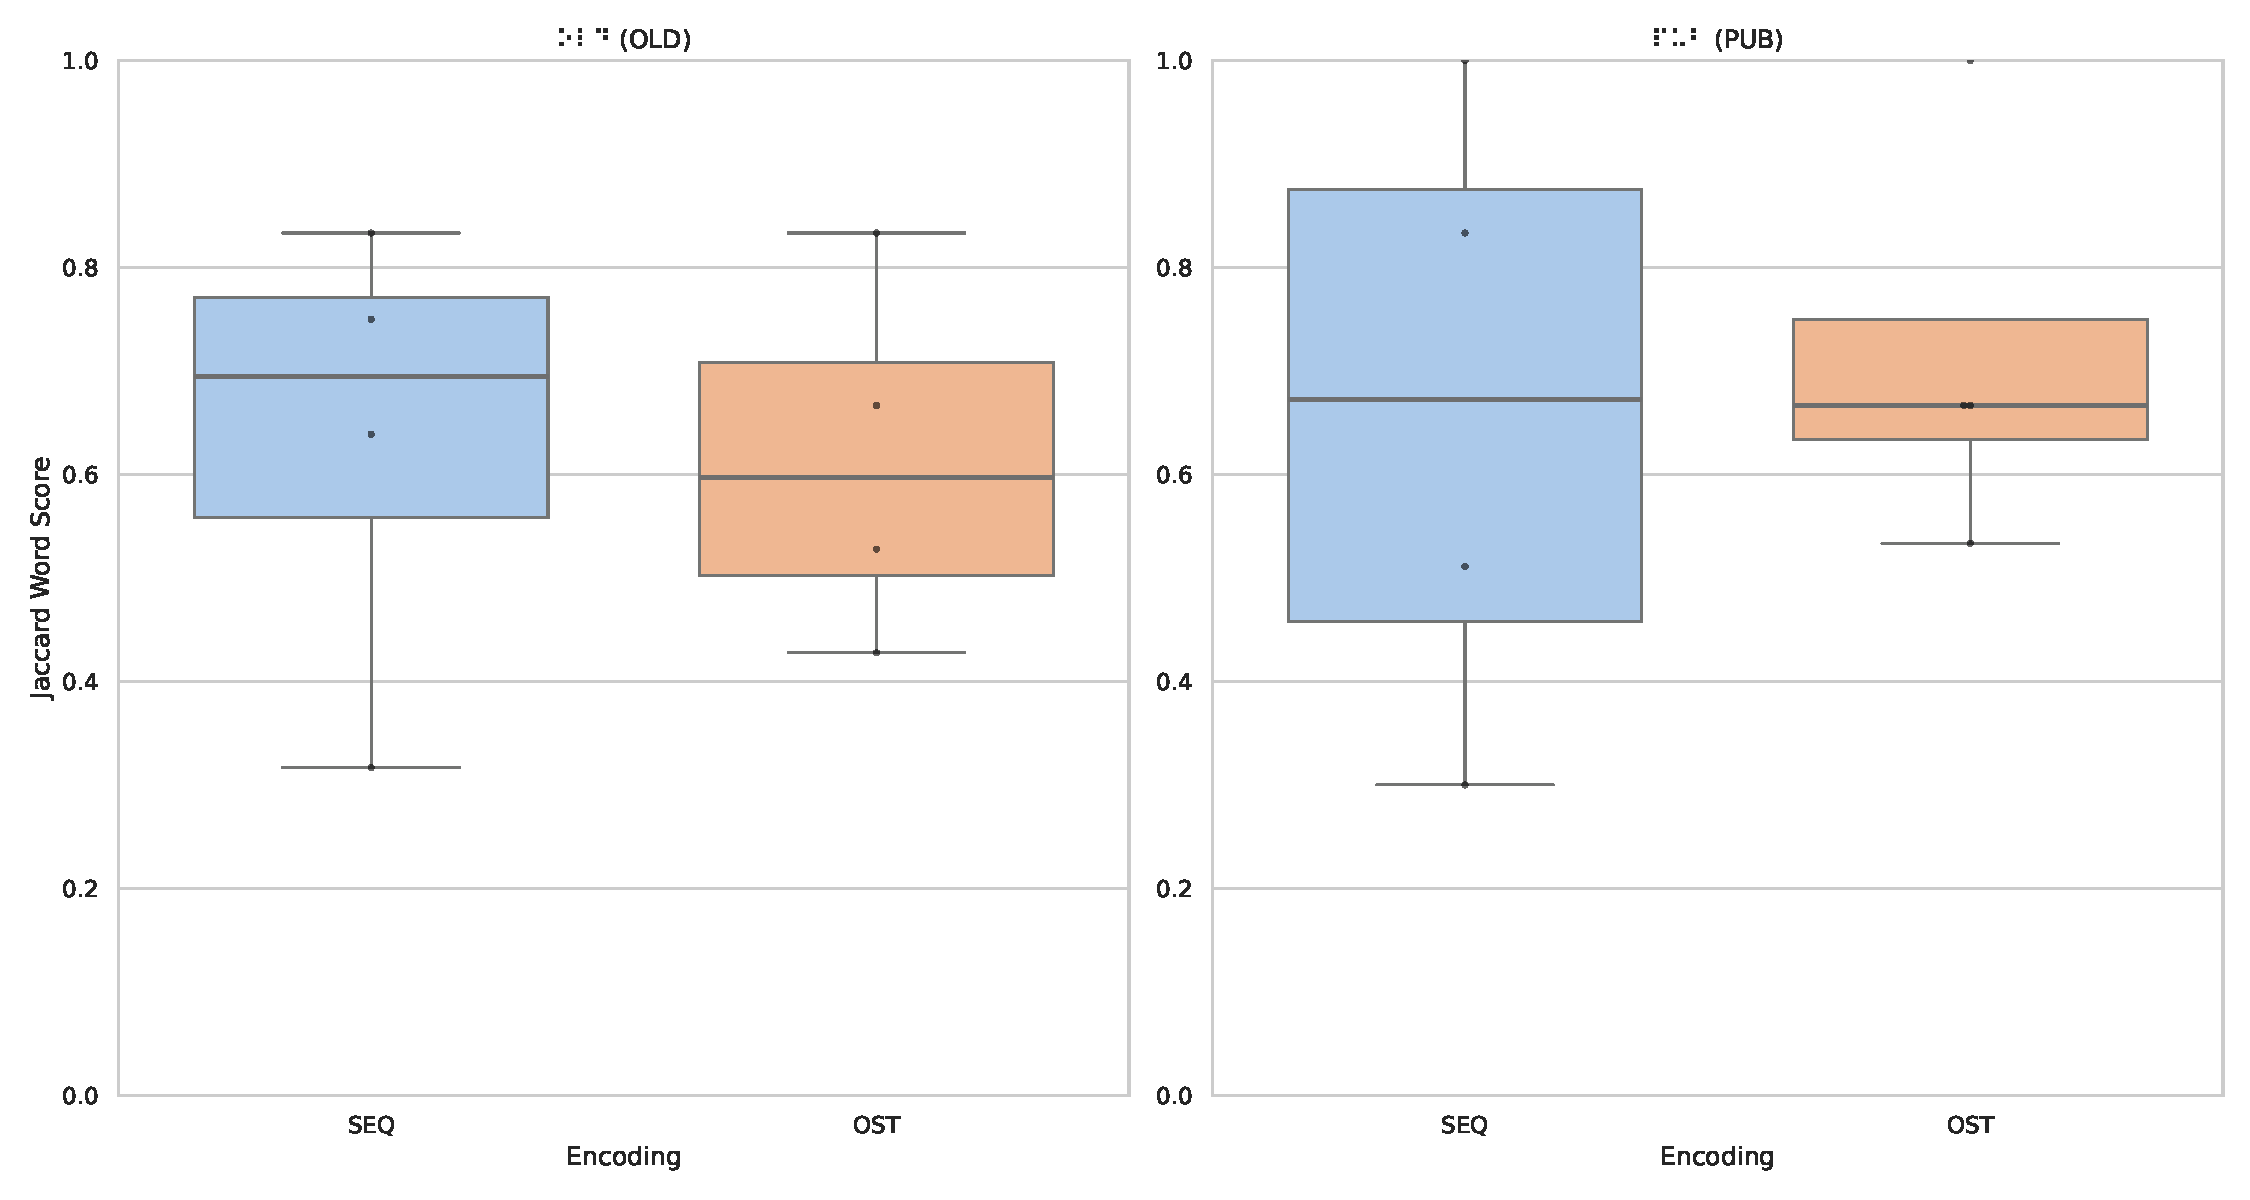
\includegraphics[width=\linewidth]{src/pictures/Study2Data_Experiment/study2_test_results.pdf}
    \caption{Jaccard Word-Test results grouped by the Braille test-words for the different stimuli.}
    \label{fig:study2_test_results-firstStudy}
\end{figure}

After learning each word using one of the encodings, we tested the word itself, with the results shown in \autoref{fig:study2_test_results-firstStudy}, to determine whether there was a significant difference in testing the entire word after learning all the individual characters.
Interestingly, no significant difference was observed in the median. However, the Q1 and Q3 values for the word "pub" differed, with an interval of $0.62$-$0.85$ for \gls{ost} compared to $0.45$-$0.875$ for \gls{seq}.
Nevertheless, the median remained the same for both encodings, at $0.675$.

We conducted \gls{mwu} tests for the resulting words, and the results showed that no p-value was close to the threshold value of $0.05$, as depicted in \autoref{table:significance_results_test_secondStudy_nonPara}. This indicates that there was no significant difference between the sets, with p-values of $1.0$ and $0.77$.

\begin{table}[ht]
\resizebox{\columnwidth}{!}{
\centering
\begin{tabular}{|l|l|l|l|l|}
\hline
\textbf{Question} & \textbf{Test Statistic} & \textbf{p-value}  &\textbf{Significance}           &\textbf{Effect Size}\\ \hline
\braille{old}(\textbf{OLD})& 8.500& 1.000&Not Significant &0.103\\ \hline
\braille{pub}(\textbf{PUB})& 6.500& 0.770&Not Significant &0.211\\\hline
\end{tabular}}
\caption{Results of the \gls{mwu} tests for significance for the different Braille tests-words with a Cohens d Effect Size.}
\label{table:significance_results_test_secondStudy_nonPara}
\end{table}


\begin{figure}
    \centering
    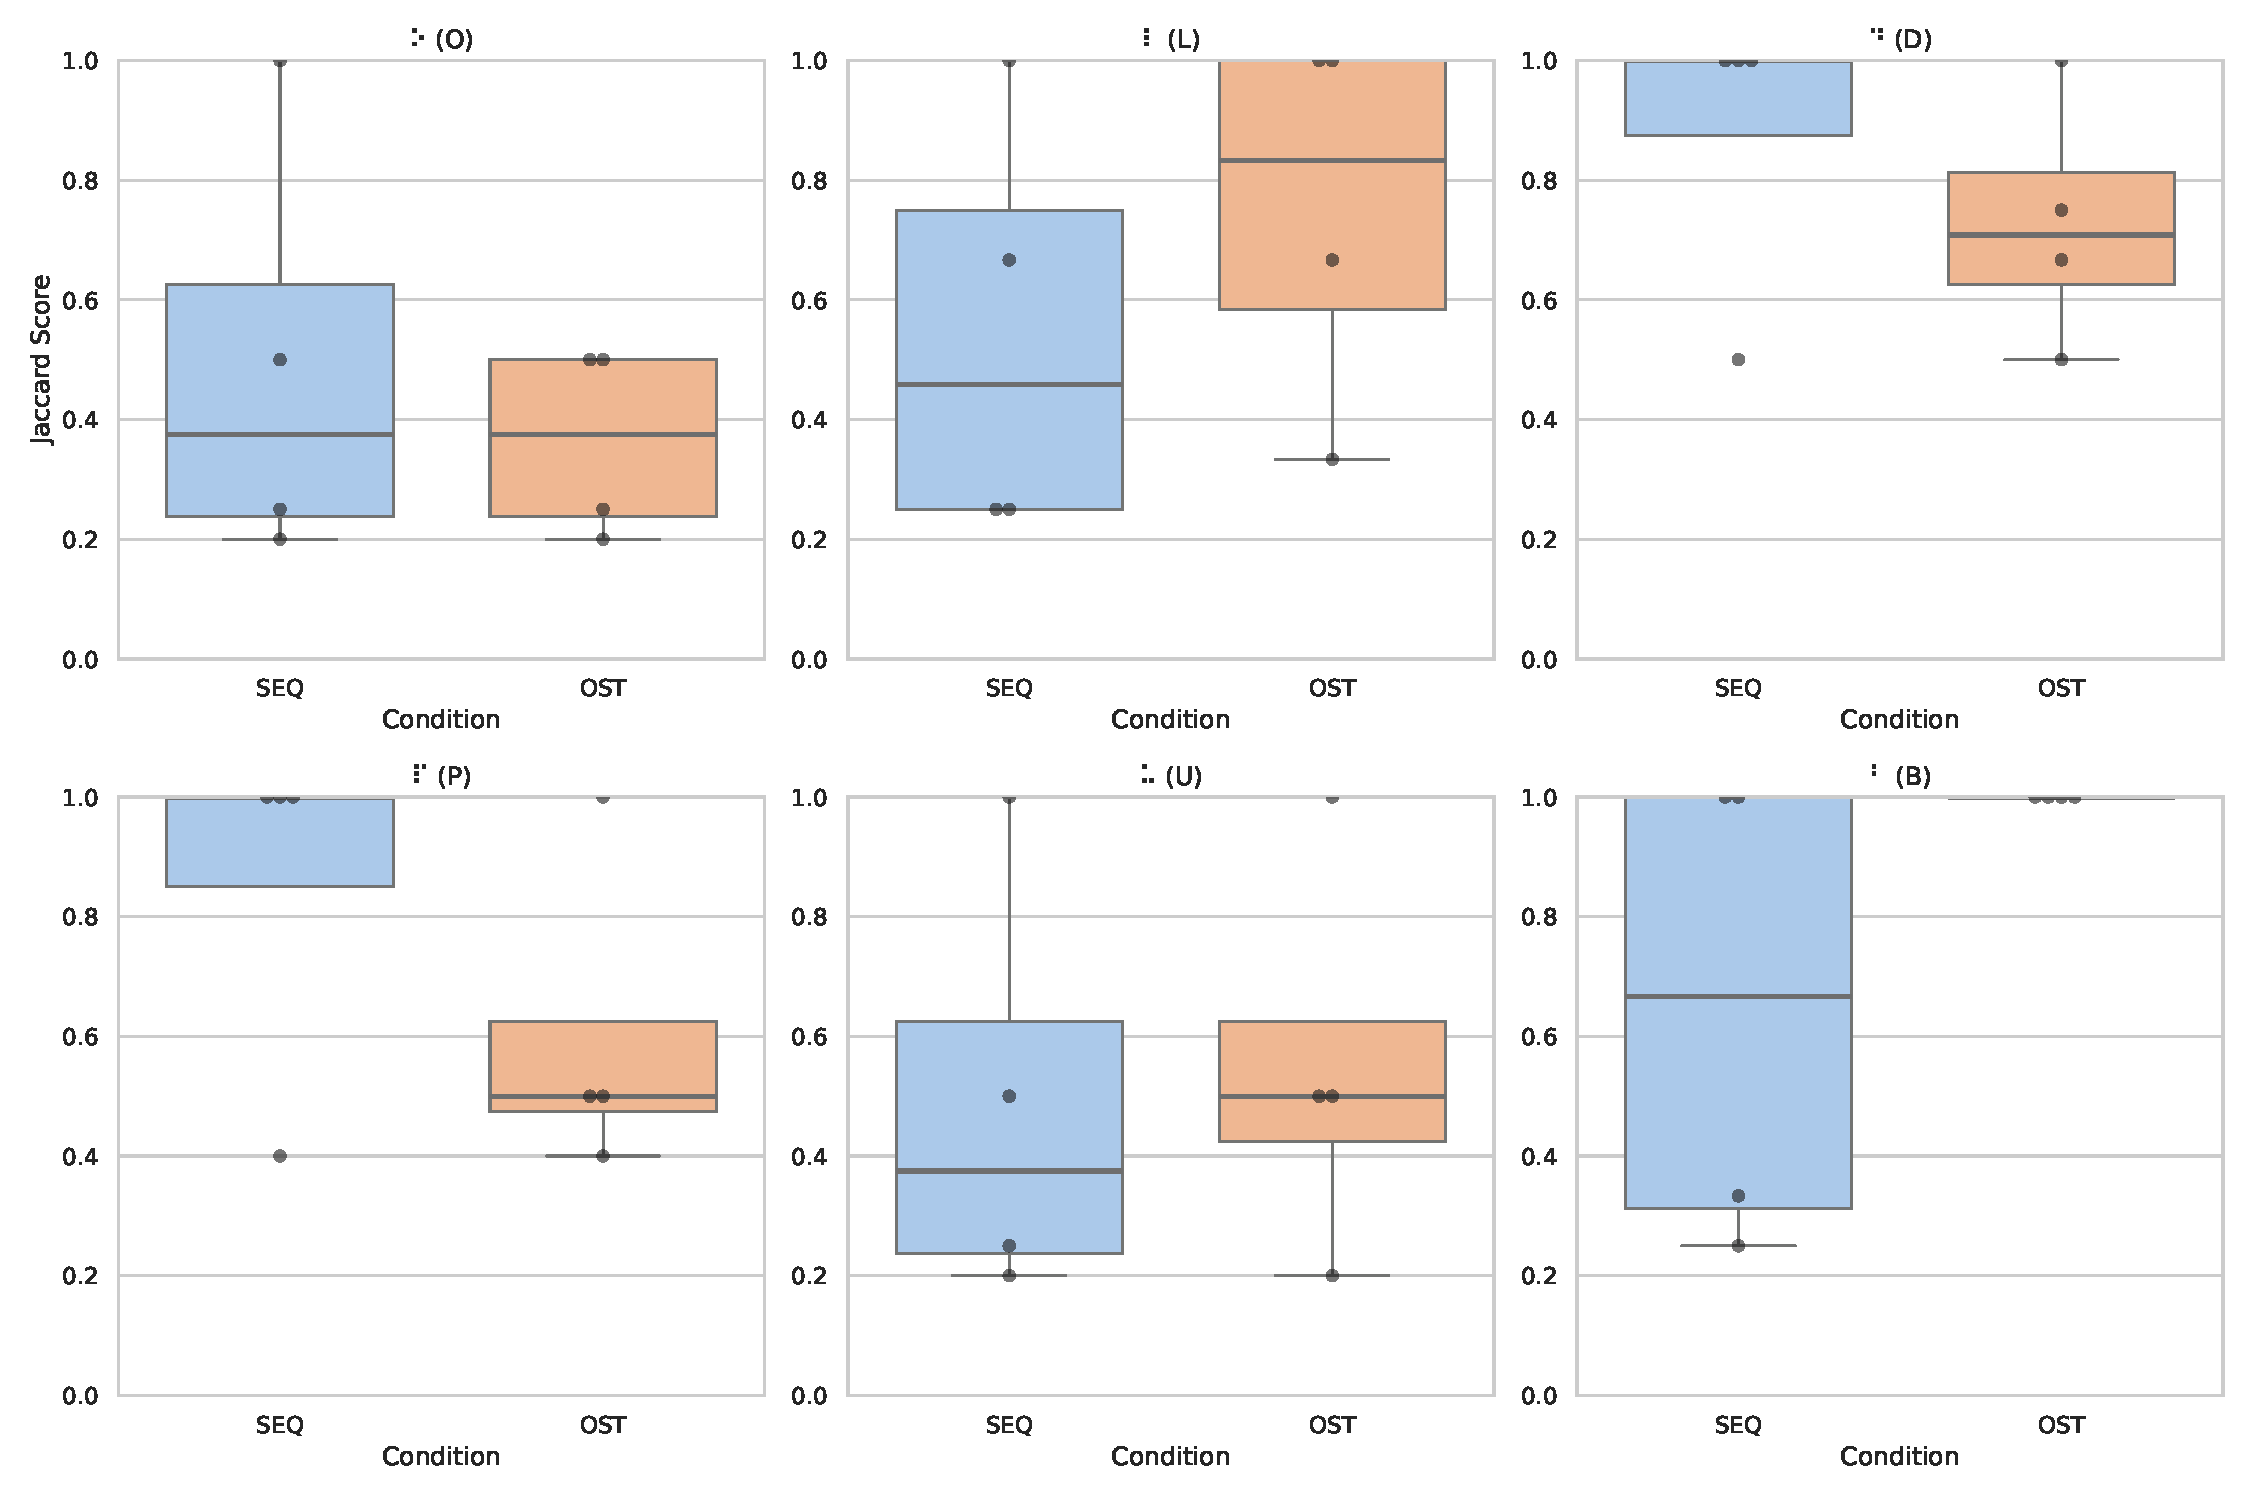
\includegraphics[width=\linewidth]{src/pictures/Study2Data_Experiment/character_jaccard_test_study2.pdf}
    \caption{Jaccard Score comparison for the different Encodings grouped by Braille character.}
    \label{fig:f1score_test_study2}
\end{figure}


\begin{table}[ht]
\resizebox{\columnwidth}{!}{
\centering
\begin{tabular}{|l|l|l|l|l|}
\hline
\textbf{Question} & \textbf{Test Statistic} & \textbf{p-value}  &\textbf{Significance}           &\textbf{Effect Size}\\ \hline
\braille{o}(\textbf{O})& 9.000& 0.881&Not Significant &0.443\\ \hline
\braille{l}(\textbf{L})& 4.500& 0.369&Not Significant &0.609\\ \hline
\braille{d}(\textbf{D})& 11.000& 0.439&Not Significant &0.634\\ \hline
\braille{p}(\textbf{P})& 11.000& 0.436&Not Significant &0.875\\ \hline
\braille{u}(\textbf{U})& 7.000& 0.881&Not Significant &0.179\\ \hline
\braille{b}(\textbf{B})& 4.000& 0.186&Not Significant &1.221\\ \hline
\end{tabular}}
\caption{Results of the \gls{mwu} for significance grouped by the different Braille characters during learning for the different Encodings with Cohen's d.}
\label{table:learning_significance_results_secondStudy_nonPar}
\end{table}

Similarly to the first study, we analyzed the Jaccard scores for the different characters in the second study. The most significant differences were observed for the characters \braille{b}(B), followed by \braille{p}(P), \braille{l}(L), and \braille{d}(D).

For the character \braille{b}(B), the \gls{ost} encoding performed better, achieving a perfect score, while the \gls{seq} encoding had a median of $0.675$ and a Q1-Q3 quantile range of approximately $0.3$ to $1$, as half of the participants did not achieve a perfect score.

In contrast, for the character \braille{p}(P), the \gls{ost} encoding performed worse, with a median around $0.5$, while \gls{seq} had a median of $1$. Similarly, for the character \braille{d}(D), the \gls{seq} encoding had a median of $1$, while \gls{ost} had a median of $0.7$. Notably, only one participant in the \gls{seq} group did not achieve a perfect score, with a score of $0.4$.

It is also worth noting that only one participant had a non-perfect score for \braille{d}(D) using the \gls{seq} encoding.

For the character \braille{l}(L), the \gls{ost} encoding had a median of approximately $0.825$, with half of the participants achieving a perfect score, whereas the \gls{seq} encoding had a median of about $0.45$.

Upon analyzing each character individually, no significant differences were found between the datasets. The lowest p-value was observed for \braille{b}(B), with a value of $0.186$, which is significantly higher than the threshold value. Therefore, the null hypothesis ($H_0$) cannot be rejected.

\begin{figure}
    \centering
    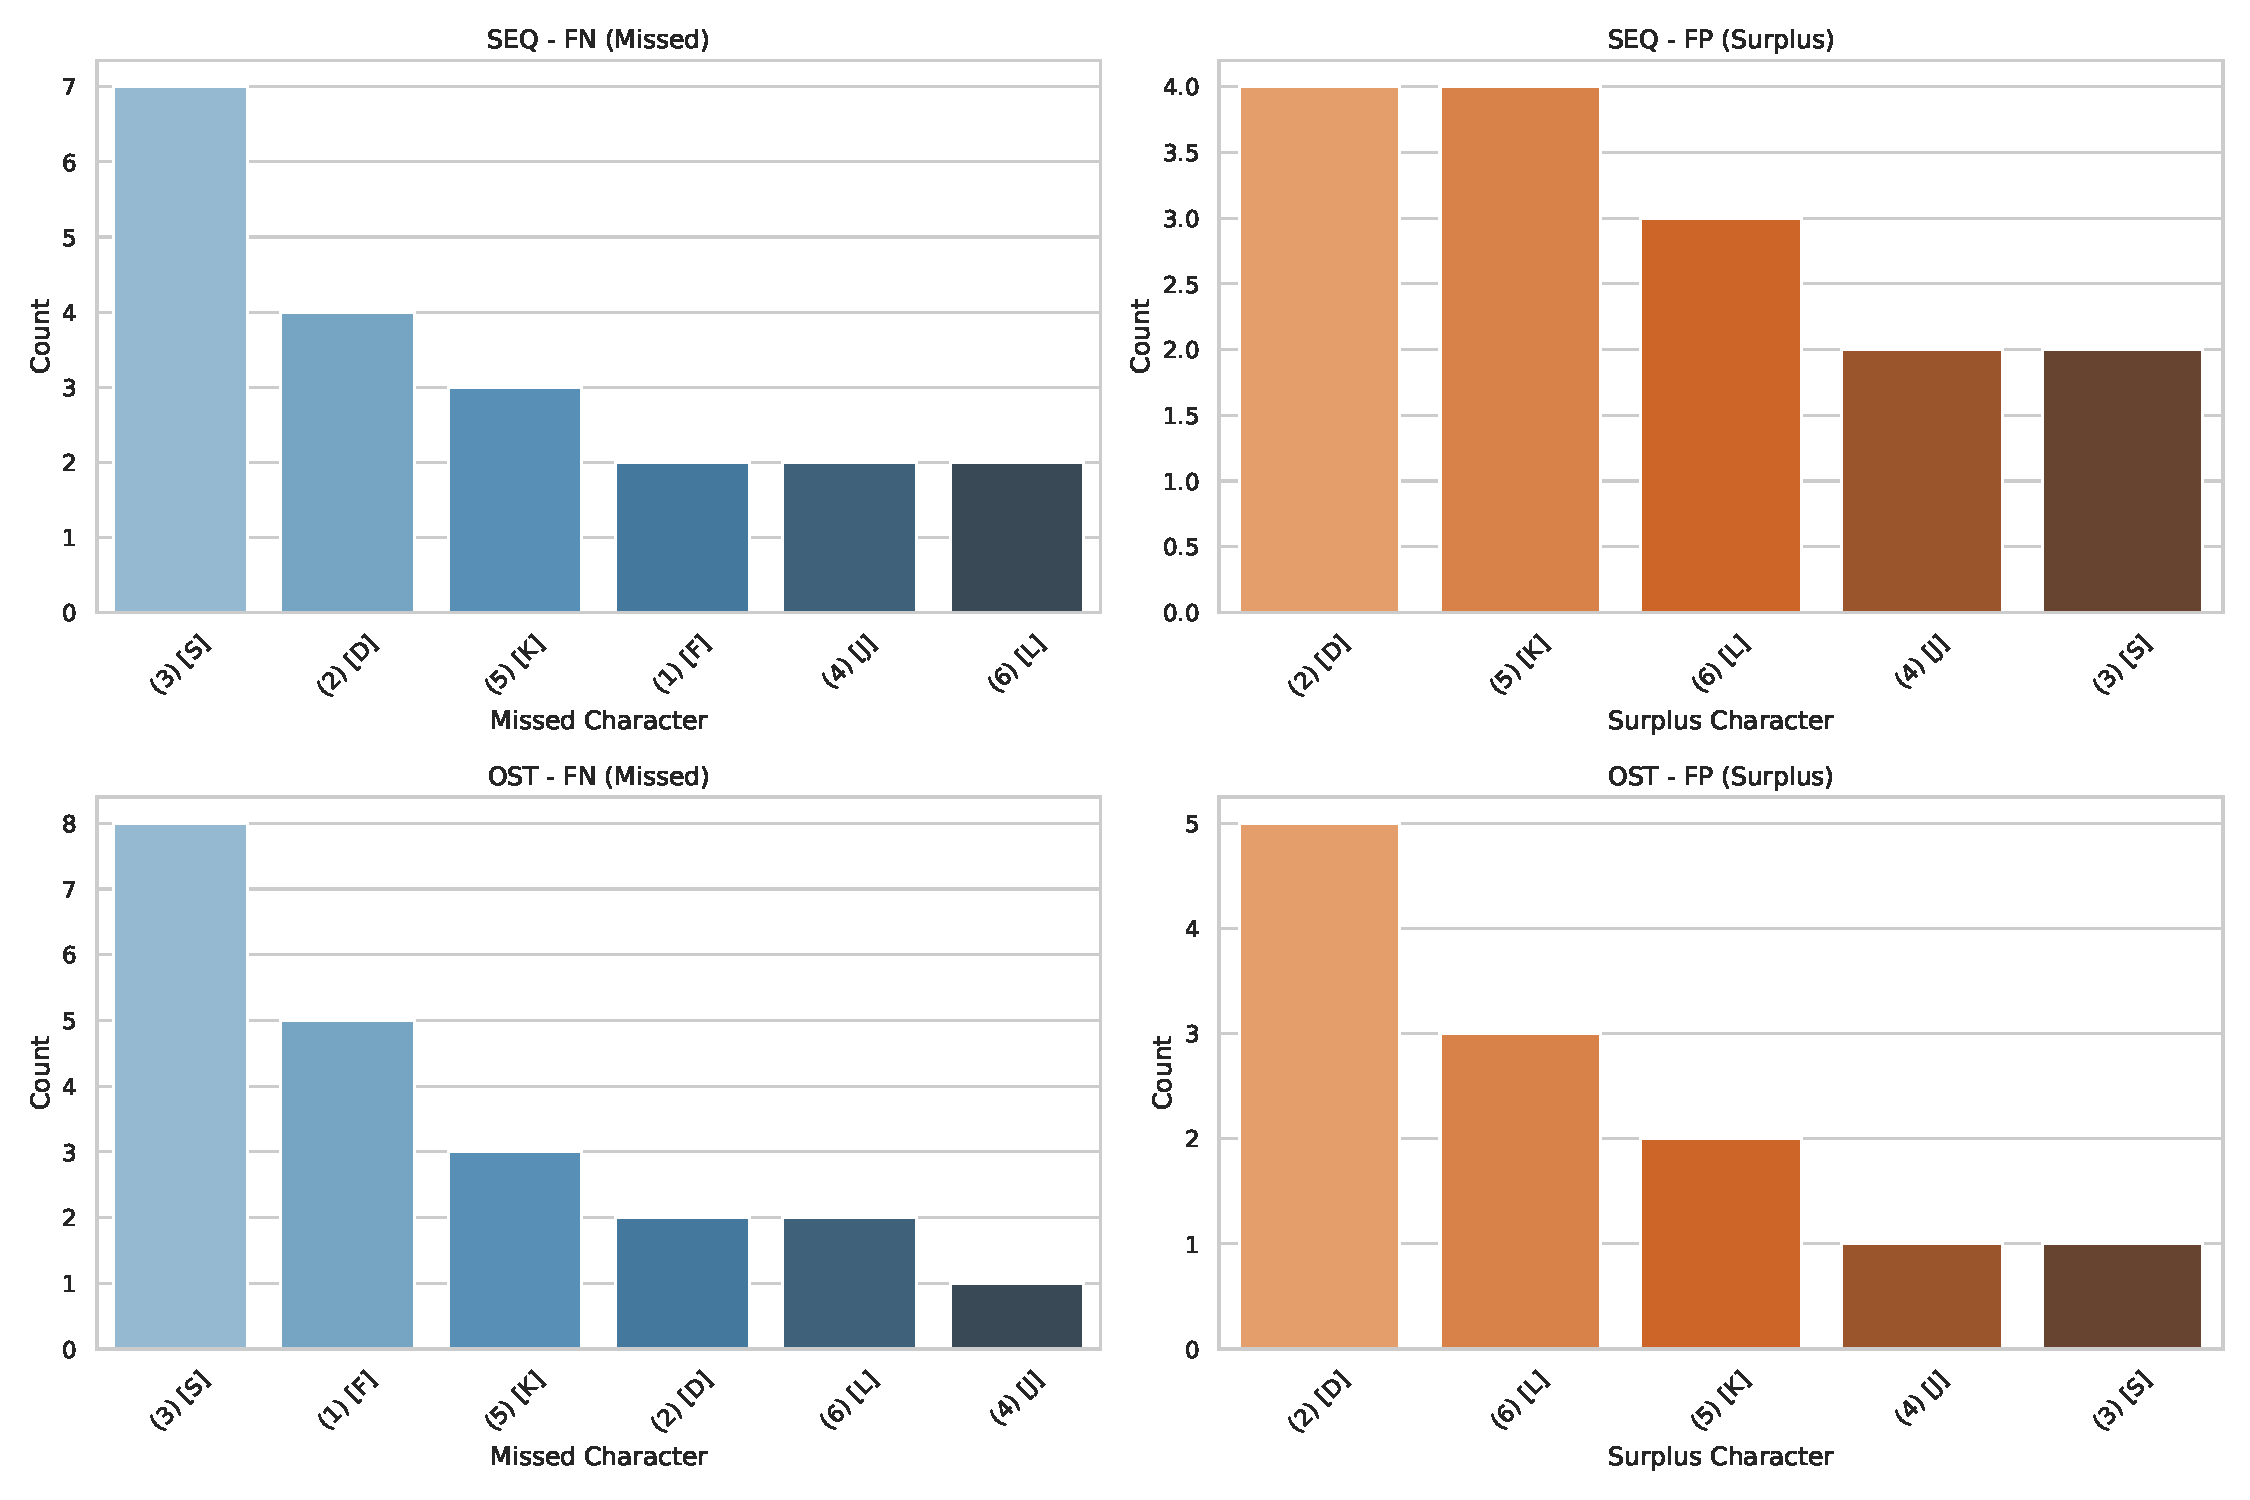
\includegraphics[width=\linewidth]{src/pictures/Study2Data_Experiment/missed_surplus_test_study2.pdf}
    \caption{FN (Missed) and FP (Surplus) Key(s) for each Braille Character by Encoding.}
    \label{fig:missedSurplus_study2}
\end{figure}

Further analysis, shown in \autoref{fig:missedSurplus_study2}, reveals that \textcircled{3} [S] is the most frequently missed character, while \textcircled{2} [D] is the most frequently in surplus. In contrast, \textcircled{4} [J] and \textcircled{6} [L] were the least missed characters, while \textcircled{2} [S] and \textcircled{4} [J] were the least in surplus.

\begin{figure}[h!]
    \centering
    \begin{subfigure}[b]{0.45\textwidth}
        \centering
        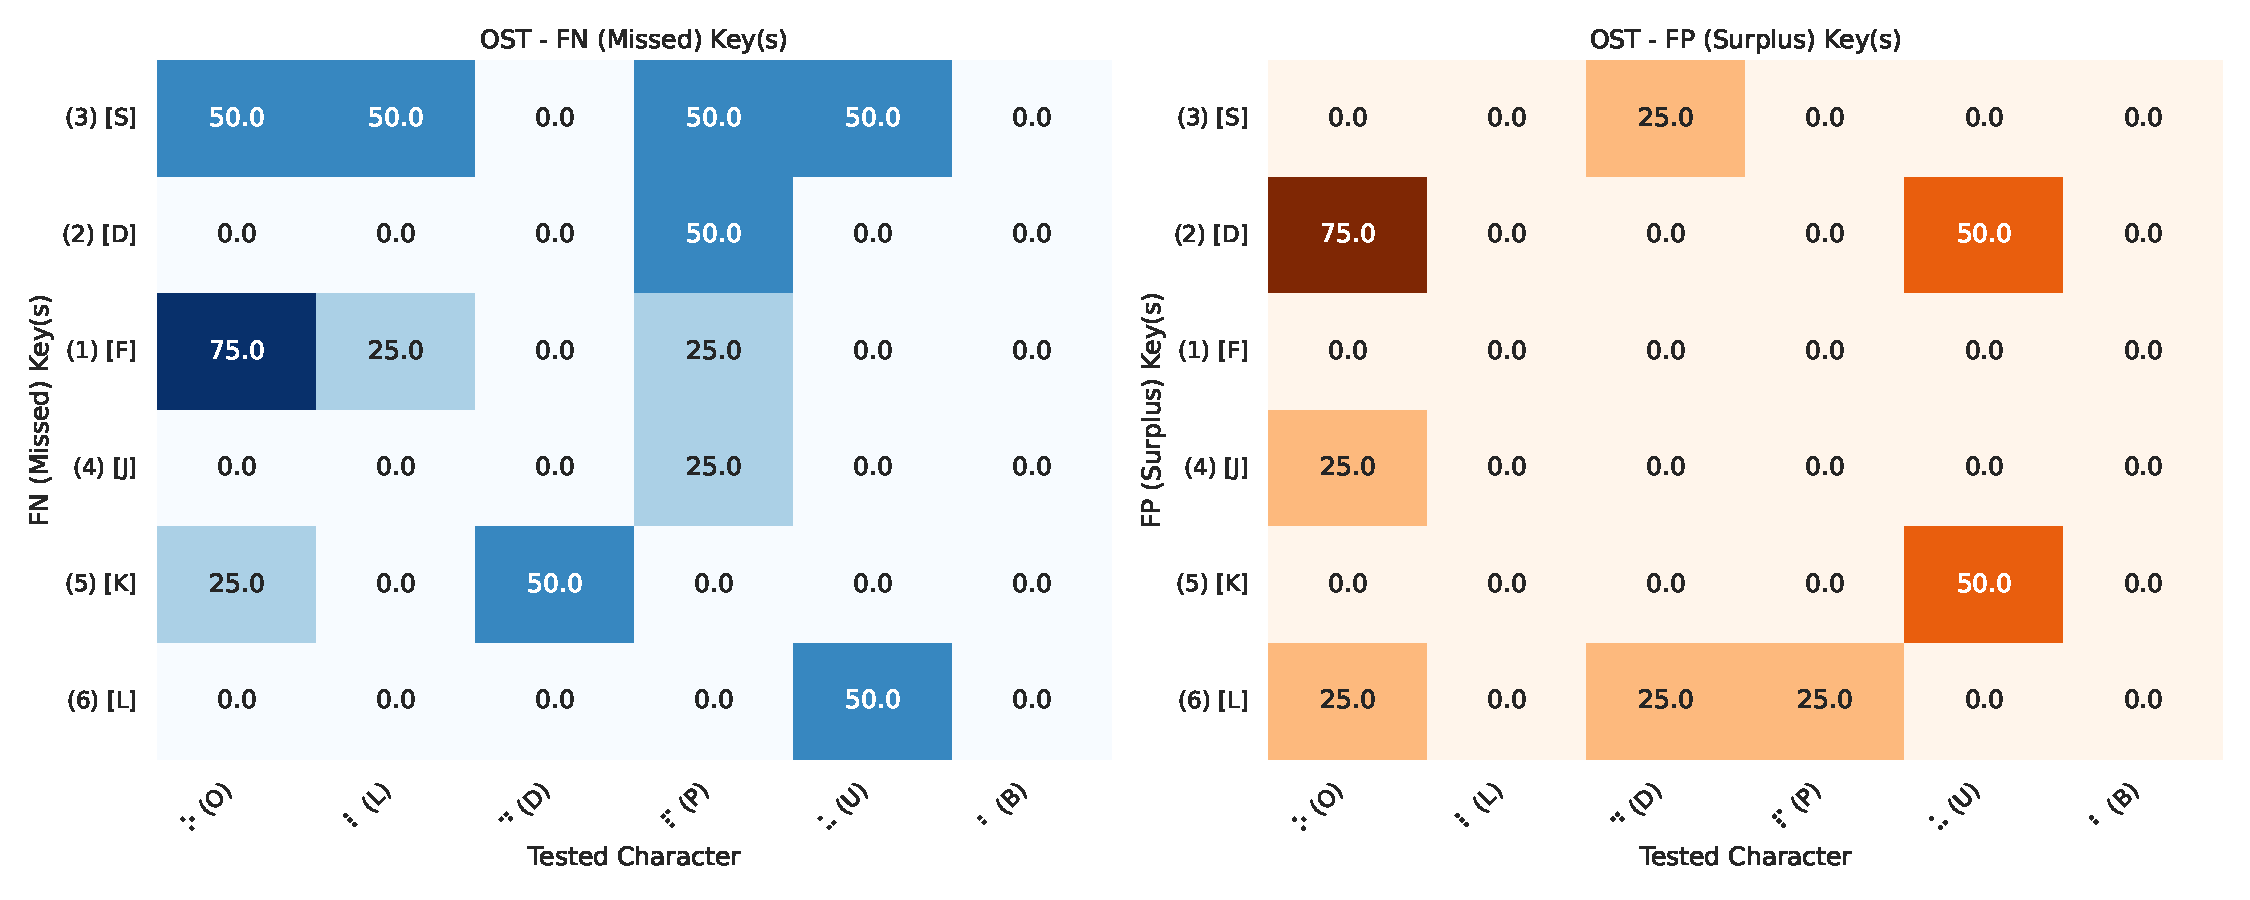
\includegraphics[width=\textwidth]{src/pictures/Study2Data_Experiment/missed_surplus_test_percentages_study2_ost.pdf}
        \caption{\gls{ost}}
    \end{subfigure}
    \begin{subfigure}[b]{0.45\textwidth}
        \centering
        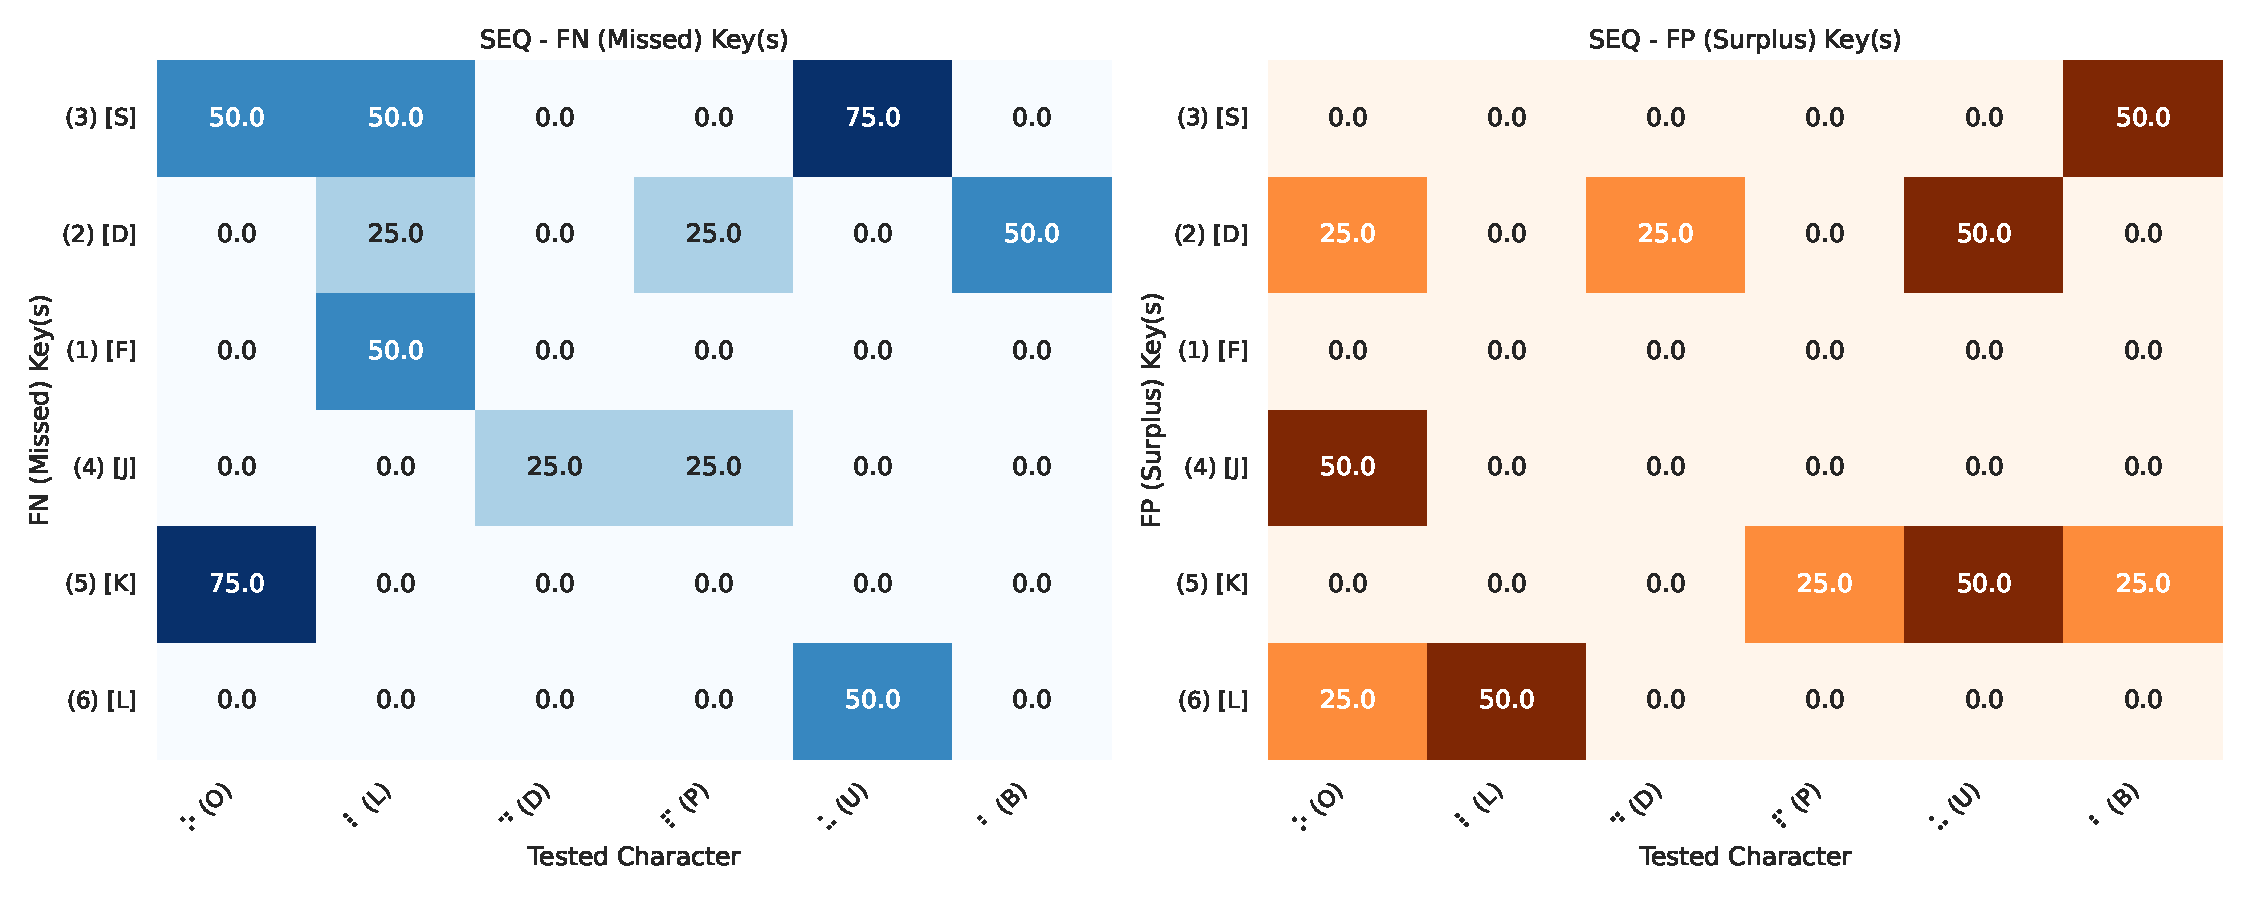
\includegraphics[width=\textwidth]{src/pictures/Study2Data_Experiment/missed_surplus_test_percentages_study2_seq.pdf}
        \caption{\gls{seq}}
    \end{subfigure}\\
    \caption{FN (Missed) and FP (Surplus) Key(s) in percent for each Braille character grouped by Encoding.}
    \label{fig:missed_surplus_percentages_study2}
\end{figure}

A closer analysis reveals that for the false positives (FP), the characters \braille{b}(B), \braille{l}(L), \braille{d}(D), and \braille{p}(P) exhibited the most notable differences.

For \braille{b}(B), the \gls{ost} encoding had no errors, while in the \gls{seq} encoding, the \textcircled{5} [K] and \textcircled{3} [S] keys were mistakenly pressed with the \textcircled{3} [S] key in 50\% of the cases.

For \braille{l}(L), there were no false positives in the \gls{ost} encoding, but half of the participants incorrectly pressed the \textcircled{6} [L] key in the \gls{seq} encoding.

For \braille{d}(D), a larger difference is evident, with 25\% of participants missing \textcircled{3} [S] and \textcircled{6} [L] in the \gls{ost} encoding, while the \textcircled{2} [D] key was incorrectly pressed in the \gls{seq} encoding.

For \braille{p}(P), the \textcircled{6} [L] key was incorrectly pressed in 25\% of the cases in the \gls{ost} encoding, while the \textcircled{5} [K] key was mistakenly pressed in the \gls{seq} encoding.

Regarding the false negatives (FN), the most significant differences were observed for the characters \braille{p}(P), \braille{b}(B), \braille{o}(O), and \braille{l}(L). 

For \braille{p}(P), the \gls{seq} encoding performed better, with only the \textcircled{4} [J] and \textcircled{2} [D] keys missed 25\% of the time. In contrast, the \gls{ost} encoding also missed the \textcircled{1} [F] and \textcircled{3} [S] keys.

For \braille{b}(B), no keys were missed with the \gls{ost} encoding, but in the \gls{seq} encoding, the \textcircled{2} [D] key was missed 50\% of the time.

For \braille{o}(O), the \textcircled{1} [F] key was missed in 75\% of the cases with the \gls{ost} encoding, while both the \textcircled{3} [S] and \textcircled{5} [K] keys were missed in both encodings. Notably, the \textcircled{5} [K] key was missed in 75\% of the cases in the \gls{seq} encoding but only 25\% of the time in the \gls{ost} encoding.

For \braille{l}(L), both the \textcircled{1} [F] and \textcircled{3} [S] keys were missed in both encodings, though the \gls{seq} encoding also missed the \textcircled{2} [D] key 25\% of the time.

Analysis of the missed keys shows the largest differences for the \textcircled{1} [F] and \textcircled{2} [D] keys. 

The \textcircled{1} [F] key was missed in the \braille{l}(L) test in the \gls{seq} encoding, and also for \braille{o}(O) and \braille{p}(P), affecting half of the characters in the \gls{ost} encoding.

For the \textcircled{2} [D] key, it was missed for \braille{l}(L), \braille{p}(P), and \braille{b}(B) in the \gls{seq} encoding, but only in 50\% of the cases for \braille{b}(B) in the \gls{ost} encoding.

\begin{figure}
    \centering
    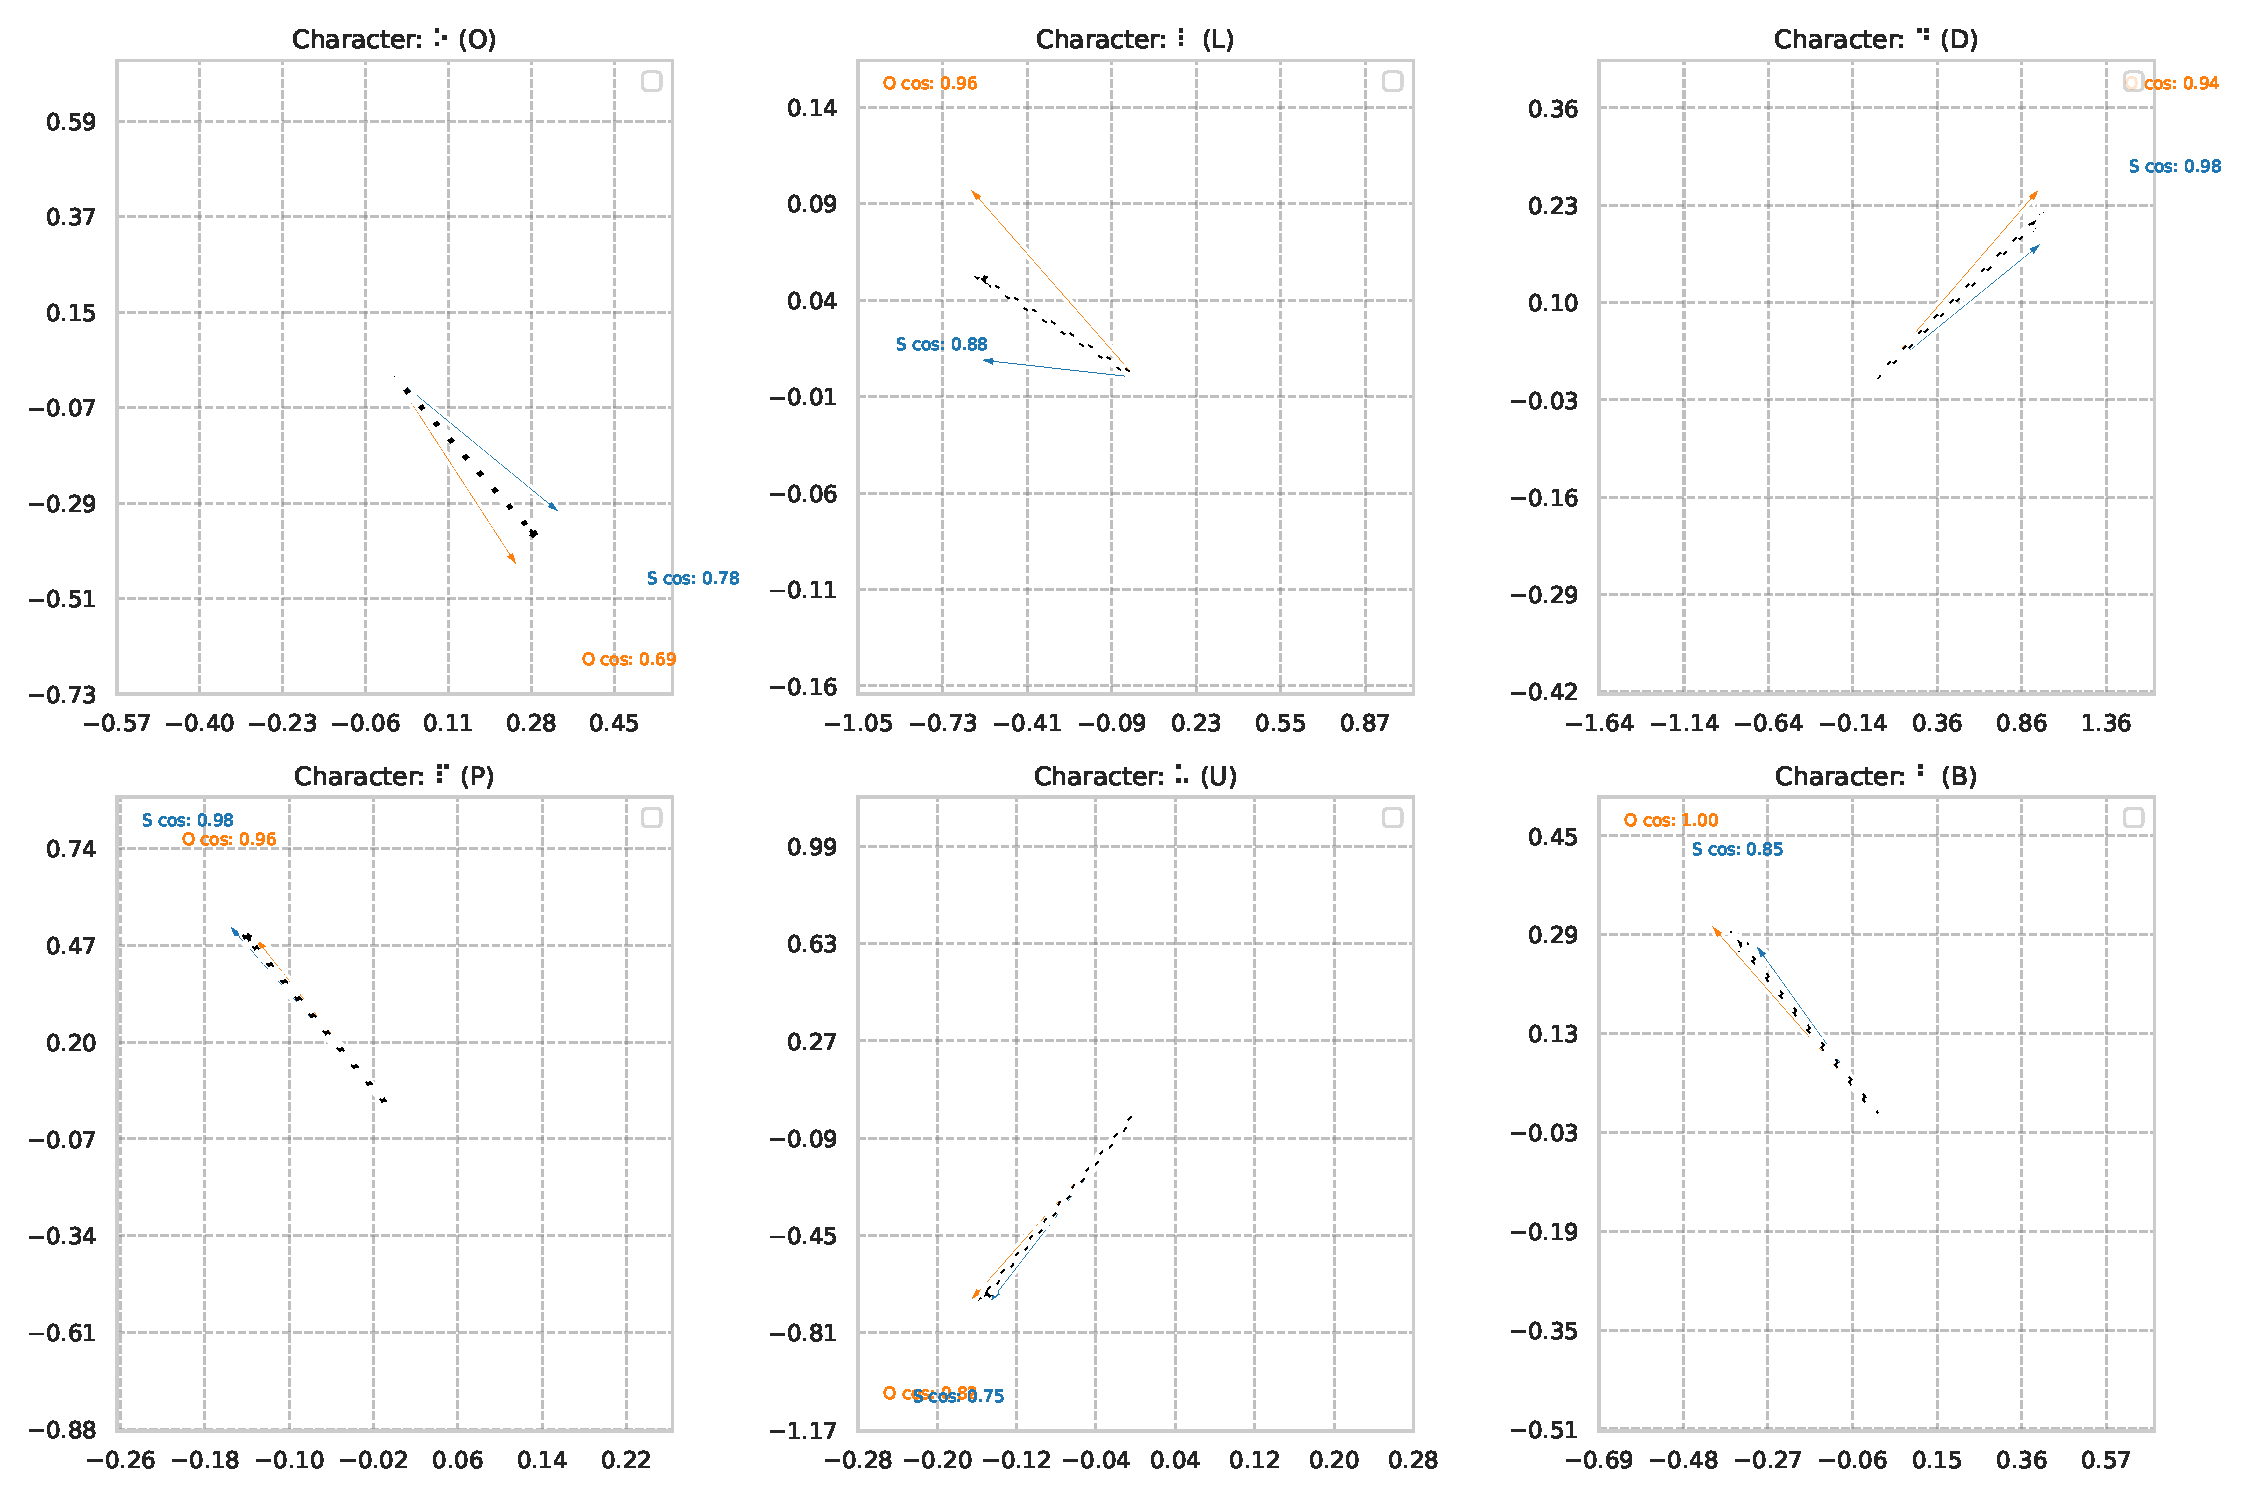
\includegraphics[width=\linewidth]{src/pictures/Study2Data_Experiment/Vectors_study2.pdf}
    \caption{Cosine Similariy for each Encoding.\\Plotted using a PCA dimensionality reduction.}
    \label{fig:cosSim_PCA_study2}
\end{figure}

The cosine similarity and \gls{pca} analysis, as shown in \autoref{fig:cosSim_PCA_study2}, indicate that despite noise reduction through \gls{pca}, the vectors align in a similar direction. The most noticeable differences were observed for the braille characters \braille{o}(O) and especially \braille{l}(L).
However, their cosine similarity scores are still rather similar with 0.69 for the \gls{ost} and 0.78 for \gls{seq} for the braille character \braille{o}(O).
For the Braille character \braille{l}(L), the cosine similarity is even smaller with 0.96 for \gls{ost} and 0.88 for \gls{seq}.
 
 \chapter{Evaluation}
\label{ch:Evaluation}

This section is used to interpret the data gathered in the analysis section and answer the two research questions \enquote{\textcolor{red}{RQ1 is there a difference for ost both hand between affective and discriminative touch}} and
\enquote{\textcolor{red}{RQ2: is ther a signifficant difference between using the ost over the seq encoding}}.

\subsection{First Study}
%NASA TLX
In the first study, we compared the task load of the participants using the NASA TLX task load index. 

By analyzing the six different task load dimensions for each stimulus, as shown in \autoref{fig:nasaTLX-firstStudy}, and testing for significant differences between the stimuli (as presented in \autoref{table:nasaTLX_significance_firstStudy}), we found no significant differences. 

However, it is evident that there is a notable difference in the median performance statistics, suggesting that the \enquote{Performance} dimension was perceived more favorably in the stroking and vibration conditions.


%SELF ASSESSMENT
After completing the NASA TLX, participants were asked to self-assess how they perceived the stimulus on various dimensions, including \enquote{Feeling Pleasant}, \enquote{Helped Learning}, \enquote{Would Have Learned Faster}, \enquote{Would Use the Actuators to Support the Learning Process}, \enquote{Able to Understand Haptic Feedback}, and \enquote{Satisfaction Overall}, as depicted in \autoref{fig:questions_individual_firstStudy}.

A Kruskal-Wallis test was conducted on these responses. The results showed that the p-value for \enquote{Satisfaction} was $0.0504$. In combination with the effect size of $\eta^2$, this indicates a borderline significant difference, particularly for the tapping stimulus. Almost half of the participants rated it as very satisfying, resulting in a better Q1-Q3 quantile range compared to the other two stimuli. This suggests that participants were generally happier with the tapping stimulus, though the difference was not statistically significant.

Furthermore, the dimension \enquote{Would Have Learned Faster} yielded a p-value of $0.0882$ and an effect size of $0.1387$, which is also borderline significant, with more participants expressing dissatisfaction with the tapping stimulus.

%SELF DECISION
After the tests were completed, participants were asked to directly compare the stimuli and select which one they perceived as the best for each of the two dimensions: \enquote{Model Most Comfortable} and \enquote{Model That Helped Most in Learning}, as shown in \autoref{fig:questionsCompare-firstStudy}. 

The results indicate that both the tapping and vibration stimuli were consistently rated better than the stroking stimulus in direct comparisons. In terms of comfort, both the tapping and vibration stimuli were perceived equally, while for learning, the tapping stimulus was preferred by $7/12$ of the participants. 

However, after conducting a \gls{csgf} and an \gls{emgf}, the results, presented in \autoref{table:statistical_tests_comparrisson_firstStudy}, reveal that the perceived differences between the stimuli were not statistically significant.


%COMMENTS
Participants were also asked to provide comments \textcolor{red}{comments cite} after the study. The comments received were as follows:

\enquote{Stroking is better than vibration, and tapping is better than stroking in both comfort and learning.}

\enquote{For vibration, it is sometimes difficult to identify which finger is vibrating.}\footnote{Translated from: \enquote{Bei Vibration ist manchmal schwer zu finden, welche Finger vibriert.}}

\enquote{The vibration was unclear, as it was difficult to tell which fingers were vibrating due to interference from other vibrators. The stroking was hard to feel.}

Lastly, \enquote{I think the tapping was the most comfortable, and I was able to distinguish the fingers. I sometimes couldn’t feel the stroker.}\footnote{Translated from: \enquote{Ich empfand den Tapper am angenehmsten und man konnte die Finger gut unterscheiden. Den Stroker habe ich manchmal nur kaum gespürt.}}

The participants' comments consistently indicate that tapping was preferred over stroking, followed by vibration. This preference seems to be due to stroking being difficult to feel and vibration being hard to distinguish. In contrast, tapping was favored for its distinguishability.


%SUMARY    
In summary, we observed that performance was perceived as better for the stroking and vibration conditions in the NASA TLX. This is likely because the tapping actuator was more difficult to grasp, with an average of three fingers being stimulated for each character. This may have confused participants due to the number of taps involved.

The second questionnaire revealed that the tapping stimulus was borderline significant for \enquote{Satisfaction}, with participants rating it as the most satisfying. This finding is further supported by the comments provided by the users.

Interestingly, participants expressed dissatisfaction with the tapping stimulus in relation to \enquote{Would have learned faster}. This may stem from the same issue observed in the NASA TLX results—too much simultaneous stimulation.

However, in the \enquote{Helped learning} dimension, the tapping stimulus was still perceived as helpful, with nearly half of the participants rating it as very helpful for learning.

In a direct comparison of which stimulus was most helpful in learning, the tapping stimulus performed better. Additionally, its comfort level was rated similarly to the vibration stimulus, suggesting that from a qualitative perspective, it is a strong contender.

The vibration stimulus faced the issue of being difficult to distinguish, while the stroking stimulus generally performed worse. It was challenging to feel and distinguish, and it also underperformed in the \enquote{Helped learning} section of the usability questionnaire.


%  NASA TLX: \enquote{Performance} was perceived better for the stroking and vibration condition. 

% CUSTOM: \enquote{Satisfaction} (borderline significant) difference for the tapping stimulus, which is has with almost half of the participants voting it is very satisfying a better q1-q3 quantile range than the other two stimuli showing the users are rather happy with the tapping stimulus, however, not significant.

%  \enquote{Would have learned faster} with a pvalue of  $0.0882$ and a Effect size of $0.1387$ is borderline significant with more people dissattisfied with the tapping stimulus.

% COMPARE: It can be seen, taht the tapping and vibration Stimulus are in a direct comparison always better than the stroking one, while both, the tapping and vibration stimulus are the same for the comfortableness, moreover, the tapping was also with $7/12$ people perceiving it better in learning.

% COMMENTS:
% Tapping > Stroking > Vibration 
% vibration unclear, stroke hard to feel
% tapping distinguishable, stroking one hard to feel

%LEARNING TEST
For the objective data, we first gathered the results from all character learning tests, which are shown in \autoref{fig:learning_results_firstStudy}. After conducting Kruskal-Wallis tests for all the Braille characters, we found that there was no statistically significant difference between the sets, with the lowest p-value of $0.1599$ for the character \braille{b}(B), as shown in \autoref{table:learning_significance_results_firstStudy}. In this case, the stroking stimulus performed worse than the other two stimuli, but the results were essentially the same for the other stimuli.

The character \braille{d}(D) also showed a p-value of $0.2311$ with an effect size of $0.2663$, which is relatively high and reflects a slight difference. Here, the stroking stimulus was again perceived as slightly worse than the other stimuli; however, this difference was also far from being statistically significant.

% B = stroking bad
% D = stroking bad

%WORD TEST
Lastly, we conducted a word test to assess performance with complete words after learning. The results are shown in \autoref{fig:test_results_firstStudy}. This analysis revealed that the stroking stimulus consistently performed worse for each word, followed by the tapping and vibration stimuli, which were similar for the word \braille{the} (THE). For the other two words, \braille{old} (OLD) and \braille{pub} (PUB), the median score was slightly better for the vibration stimulus, though the difference was small.

However, no statistical significance was found, as detailed in \autoref{table:significance_results_test_firstStudy}, where the lowest p-value was $0.1371$ for the word \braille{old} (OLD). It was also noted that there was always at least one participant who achieved the best score with tapping. In general, tapping performed better than the other two stimuli for the outliers, except for the word \braille{THE}.

Vibration also performed well, ranking second for the words \braille{old} and \braille{pub} when considering the best performers.

% Stroking worse every time
% vibraiton best two times

After further analyzing the data, we found that for the \braille{l} (L) character, tapping performed the best, with no errors, followed by stroking, which also had some participants who made no errors.

For the \braille{b} (B) character, vibration outperformed both tapping and stroking, and this difference was borderline significant.

An interesting observation was that when all fingers on one hand needed to be stimulated, tapping appeared to be better than vibration, likely due to its higher distinguishability.

% L = tapping best (no errors), stroking words
% B = vibration l> tapping > strokign (For B borderline significant)

% General worst character is the E for all of the actuators, interesting because o looks similar in braille
% and for those characters all performed roughly the same bad

% when there are all fingers stimulate don one hand, tapping seems to be better than vibarion due to the distinguishability

%ERROR ANALYSIS

The error analysis revealed that the errors were mostly consistent across stimuli. For false negatives (FN), the most frequent error was \textcircled{1} [F], followed by \textcircled{3} [S] and \textcircled{5} [K] for both vibration and tapping, and \textcircled{2} [D] and \textcircled{5} [K] for stroking. The least frequent false negative was \textcircled{6} [L].

The false positives (FP) also showed similar patterns. The most frequently added character was \textcircled{6} [L], while the least frequent false positive was \textcircled{1} [F].

This indicates that \textcircled{6} [L] was pressed almost constantly, even when not needed for some characters, while \textcircled{1} [F] was pressed less often and was mostly missed across all actuators.

%Detailled
A detailed analysis revealed that the errors were similar for both the vibration and stroking stimuli. For example, in the case of the character \braille{u}(U), the \textcircled{5} [K] key was pressed incorrectly for both stimuli. However, for the vibration stimulus, the \textcircled{4} [J] and \textcircled{2} [D] keys were also pressed incorrectly.

In terms of false negatives (FN), the \textcircled{6} [L] character was never missed with the vibration stimulus but was missed in 1/4 of the cases for tapping and stroking.

This analysis concludes that the tapping and vibration stimuli performed similarly overall, while the stroking stimulus appeared to perform slightly worse. Based on both the quantitative and qualitative data, we found no statistically significant difference between two-handed \gls{ost} encoding for affective versus discriminative touch stimuli. Nevertheless, there is a small difference indicating that both the tapping and vibration stimuli were slightly more effective, both in terms of performance and the perceived usefulness reported by participants.


\subsection{Second Study}
The second study was conducted to see the differences between the different encodings \gls{ost} and \gls{seq}.

%NASA TLX
Similarly to the first study, we analyzed the subjective feelings of the participants using the NASA TLX. The results are shown in \autoref{fig:nasaTLX-secondStudy}, and the statistical significance of these results is presented in \autoref{table:nasaTLX_significance_secondStudy}.

As shown in the plot and table, there is no significant difference between the two encodings, as measured by the Mann-Whitney U test (\gls{mwu}), with all p-values being above 0.4.

This indicates that both encodings resulted in similar task load perceptions.
%same task load

%SELF ASSESSMENT
The self-assessment results of the participants, shown in \autoref{fig:questions_individual_secondStudy} and the corresponding significance tests tabulated in \autoref{table:individualQuestions_significance_secondStudy}, reveal no significant difference between the perceived quality of the different encodings, suggesting that they are essentially the same.

However, there is one notable difference in the \enquote{Feeling Pleasant} category, where the \gls{seq} encoding had a median of 3, while the \gls{ost} encoding scored a 4.

For the \enquote{Satisfaction} dimension, a larger difference can be observed in the Q1-Q3 quantile range, but this is attributed to one participant who rated the \gls{seq} encoding as more satisfying and did not provide a score of 3. Therefore, the encodings are effectively the same, as reflected by the p-value of 0.7 for this dimension.

%DIRECT COMPARE
The direct comparison, shown in \autoref{table:statistical_tests_comparrisson_secondStudy}, indicates that the \gls{seq} encoding was rated better for \enquote{Better distinguishable encoding} and \enquote{Helped learning encoding}, with 5/8 participants rating it higher for both categories. However, for \enquote{Most comfortable encoding}, the \gls{ost} encoding scored worse, with 3/8 participants rating it lower.

None of these differences were statistically significant, as indicated by the p-value of 0.4795 for all dimensions..

%SUMMARY
In general, there is no significant difference between the two encodings in terms of the participants' self-assessment. This is true both for the task load measured by the NASA TLX and the self-assessment questionnaire, where neither dimension showed statistically significant differences.

Additionally, the direct comparison of which encoding was perceived as better after the study was not significant, as the differences were limited to just one participant per dimension. Therefore, none of the qualitative assessments showed significant differences.


%Learning results
After the characters were learned using one of the encodings, we conducted tests, with the Jaccard results shown in \autoref{fig:learning_results_secondStudy} and the results of the \gls{mwu} significance tests tabulated in \autoref{table:learning_significance_results_secondStudy_nonPar}.

An observed difference was tested using the character \braille{p}(P), which showed a Cohen's d effect size of $1.492$, with the \gls{seq} encoding performing better. For the character \braille{d}(D), the \gls{seq} encoding also performed better, with a median of 1 compared to the \gls{ost} encoding, which had a median of $0.425$.

For the characters \braille{l}(L) and \braille{u}(U), the \gls{ost} encoding performed better. Interestingly, for all Braille characters containing \textcircled{4} (J) or \textcircled{5} (K), the \gls{seq} encoding outperformed the \gls{ost}.


%TEST
After learning all the words, the word test was conducted, and the results are depicted in \autoref{fig:study2_test_results-firstStudy}. The significance tests are tabulated in \autoref{table:significance_results_test_secondStudy_nonPara}.

As seen from the significance tests, with p-values over 0.7, there is no significant difference between the encodings. Additionally, the plot shows that the worst-performing \gls{seq} encoding performed worse for both words than the worst-performing \gls{ost} encoding. However, the best-performing \gls{seq} encodings resulted in slightly better participant scores than the best \gls{ost} encodings, indicating a wider variance in performance.

%CHARACTER ANALYSE
We then analyzed the individual characters as before, which are plotted in \autoref{fig:f1score_test_study2}, with their significance tests tabulated in \autoref{table:learning_significance_results_secondStudy_nonPar}.

As shown, there are larger differences for the characters \braille{b}(B), \braille{p}(P), \braille{l}(L), and \braille{d}(D); however, none of these differences were statistically significant.


%ERRORS
We then tested the false positives (FP) and false negatives (FN) for each of the characters, as shown in \autoref{fig:missedSurplus_study2}.

The results indicate that many of the FN errors were associated with \textcircled{3} [S]. For the FP errors, both encodings showed \textcircled{2} [D], \textcircled{5} [K], and \textcircled{6} [L].


%CHARACTER CHECKS
We then analyzed the errors for each character, with the plots available in \autoref{fig:missed_surplus_percentages_study2} for both the seq and ost encodings.

The analysis of the plots revealed differences for FP in the characters \braille{b}(B), \braille{l}(L), and \braille{d}(D). For FN, the differences were observed in the characters \braille{o}(O), \braille{l}(L), \braille{p}(P), and \braille{b}(B).

The largest differences for FN were seen with the Braille character \braille{p}(P), where the keys \textcircled{3} [S] and \textcircled{1} [F] were often missed. For FP, the largest differences were with the Braille character \braille{b}(B), where the keys \textcircled{3} [S] and \textcircled{5} [K] were pressed too frequently.


%COMMENTS
The comments evaluating the different encoding schemes were:
\enquote{For OST, I don't perceive the vibration as accurately.},
\enquote{I had difficulties to register which finger did vibrate.},
\enquote{If I had to learn with one method with the goal of having learned something in the end, I would choose SEQ. If it's just for fun, I would choose OST.},
\enquote{I had difficulties to register which finger did vibrate.},
\enquote{OST was easier to ignore. SEQ was harder to ignore, more irritating during the game.},
\enquote{In the second section, I learned the Braille better because the devices of each finger didn’t vibrate at the same time.},
This shows that the users seem to prefer the \gls{seq} encoding over the \gls{ost} by saying it is more distinguishable.






%SUMMARY
In general, there are no significant differences between the encodings. However, the \gls{seq} encoding was slightly better than the \gls{ost} encoding in the tests, and the comments were more positive regarding \gls{seq}. Nevertheless, the direct comparison revealed that there is no large difference between the two encodings. Some participants expressed strong opinions against \gls{seq} due to its distinguishability, while others preferred it for being more comfortable. This suggests that both encodings are valuable for passive haptic learning. Additionally, there appears to be no substantial difference in the number of repetitions between the two encodings. Although the \gls{ost} encoding involved more repetitions, the \gls{seq} encoding did not result in a higher number of repetitions within the same time frame, as the \gls{ost} encoding was faster. Therefore, we conclude that time, rather than the number of repetitions, is the key difference between the two encodings.


\subsection{Threats to validity}
\section{Threats to Validity}

We identified several potential threats to validity in both of our studies, which are categorized into internal, external, and construct validity, following the framework outlined by Lago et al. \cite{10.1145/3674805.3686691} which are illustrated in \autoref{fig:threats_to_validity}.

\subsection{Internal Validity}
One key threat to internal validity is the sample size. In the \textbf{first study}, an \textit{a priori} power analysis using the g* power software determined that a sample size of \textbf{36} was required to achieve \textbf{80\% power}. However, only \textbf{12} samples were used, and a \textit{post hoc} power analysis revealed an achieved power of only \textbf{0.34}. This low statistical power increases the risk of a \textbf{Type II error}, meaning that true effects may not have been detected. 

Similarly, in the \textbf{second study}, the \textit{a priori} power analysis indicated that a sample size of \textbf{45} was necessary for adequate statistical power. However, the \textit{post hoc} power analysis showed that the actual power achieved was only \textbf{0.356}. These findings suggest that both studies were underpowered, limiting the reliability of their conclusions.

Additionally, we used a relatively young participant group, with a median age of \textbf{28.67 years} in the first study and \textbf{24.5 years} in the second study. Both studies also included only \textbf{one left-handed participant}. Furthermore, the gender distribution was imbalanced, with only \textbf{three female participants} in each study. This lack of diversity may limit the generalizability of our findings across different populations.

\subsection{External and Construct Validity}
Hand size emerged as a potential factor affecting external and construct validity. Differences in hand size may influence the placement of actuators, as they could sit differently on individuals with larger or smaller hands. This variation in actuator positioning could have introduced slight inconsistencies in the stimuli delivered, potentially influencing our results.

Another construct validity concern relates to stimulus perception. Some participants reported that they did not perceive the \textbf{stroking stimulus} as effectively as the \textbf{vibration} or \textbf{tapping} stimuli. This perception discrepancy could impact the interpretation of the stimulus' effects and must be considered when evaluating the results.

Lastly, none of the participants were native English speakers. Although the words used in the experiments were simple, short, and commonly encountered, some participants may have had minor spelling difficulties. However, we consider this issue to have a negligible impact on the overall findings.




\begin{figure}
    \centering
    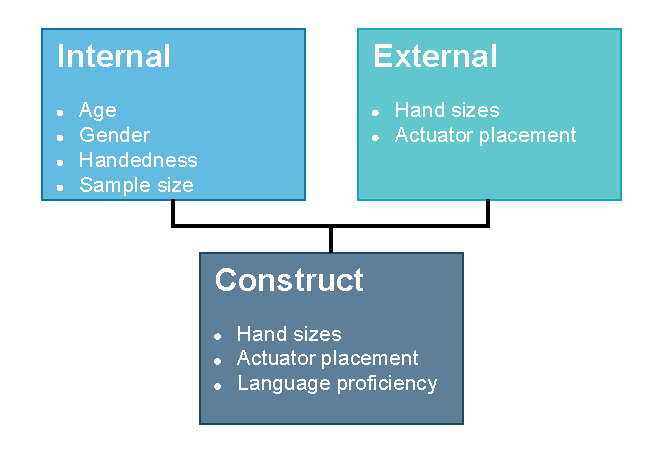
\includegraphics[width=0.5\linewidth]{src/pictures/StudyData/Threats_to_validity.drawio.pdf}
    \caption{Threats to validity}
    \label{fig:threats_to_validity}
\end{figure}




 
 
\chapter{Conclusion and Future Work}
\label{ch:conclusion}

In future studies, tapping as a stimulus could be further explored for passive haptic learning, as it is not yet commonly utilized. Additionally, the interaction between audio and vibration offsets, as well as the length of stimulus activation, presents an interesting area for investigation. The current setup could also be adapted to explore the potential for learning two-handed instruments, such as the flute, using passive haptic learning with chorded pieces or even other activities that require multi-finger coordination.

Another direction for future research involves testing the \gls{seq} encoding with the tapping stimulus to determine whether the combination of these two factors yields a slightly better learning outcome compared to other encoding methods. While our current findings suggest that time, rather than the number of repetitions, is a key factor in the efficacy of different encodings, further studies are needed to investigate this relationship in greater detail.

Additionally, the relatively low error rate in single-finger tasks opens up the possibility of employing artificial intelligence to predict the braille characters, which could potentially shorten the learning time for braille. It would also be valuable to explore whether different teaching methods can better drill muscle memory for braille learning using \gls{phl}. These avenues could provide deeper insights into the optimization of passive haptic learning systems and their application in diverse learning contexts.

 
\chapter{Summary}
\label{ch:Summary} 

%% ----------------
%% |   Appendix   |
%% ----------------

\appendix
%\include{src/appendix/anhang_a}
%\include{src/appendix/anhang_b}

%% --------------------
%% |   Bibliography   |
%% --------------------

\cleardoublepage
\phantomsection
\addcontentsline{toc}{chapter}{\bibname}
\printbibliography

\end{document}
%% --------------------------------------------------------------------------------
%% |                              END OF DOCUMENT                                 |
%% --------------------------------------------------------------------------------